% Options for packages loaded elsewhere
\PassOptionsToPackage{unicode}{hyperref}
\PassOptionsToPackage{hyphens}{url}
\PassOptionsToPackage{dvipsnames,svgnames,x11names}{xcolor}
%
\documentclass[
  a4paperpaper,
]{scrbook}

\usepackage{amsmath,amssymb}
\usepackage{iftex}
\ifPDFTeX
  \usepackage[T1]{fontenc}
  \usepackage[utf8]{inputenc}
  \usepackage{textcomp} % provide euro and other symbols
\else % if luatex or xetex
  \usepackage{unicode-math}
  \defaultfontfeatures{Scale=MatchLowercase}
  \defaultfontfeatures[\rmfamily]{Ligatures=TeX,Scale=1}
\fi
\usepackage{lmodern}
\ifPDFTeX\else  
    % xetex/luatex font selection
\fi
% Use upquote if available, for straight quotes in verbatim environments
\IfFileExists{upquote.sty}{\usepackage{upquote}}{}
\IfFileExists{microtype.sty}{% use microtype if available
  \usepackage[]{microtype}
  \UseMicrotypeSet[protrusion]{basicmath} % disable protrusion for tt fonts
}{}
\makeatletter
\@ifundefined{KOMAClassName}{% if non-KOMA class
  \IfFileExists{parskip.sty}{%
    \usepackage{parskip}
  }{% else
    \setlength{\parindent}{0pt}
    \setlength{\parskip}{6pt plus 2pt minus 1pt}}
}{% if KOMA class
  \KOMAoptions{parskip=half}}
\makeatother
\usepackage{xcolor}
\usepackage[left=1in, right=1in, top=1in, bottom=1in]{geometry}
\ifLuaTeX
  \usepackage{luacolor}
  \usepackage[soul]{lua-ul}
\else
  \usepackage{soul}
  
\fi
\setlength{\emergencystretch}{3em} % prevent overfull lines
\setcounter{secnumdepth}{5}
% Make \paragraph and \subparagraph free-standing
\makeatletter
\ifx\paragraph\undefined\else
  \let\oldparagraph\paragraph
  \renewcommand{\paragraph}{
    \@ifstar
      \xxxParagraphStar
      \xxxParagraphNoStar
  }
  \newcommand{\xxxParagraphStar}[1]{\oldparagraph*{#1}\mbox{}}
  \newcommand{\xxxParagraphNoStar}[1]{\oldparagraph{#1}\mbox{}}
\fi
\ifx\subparagraph\undefined\else
  \let\oldsubparagraph\subparagraph
  \renewcommand{\subparagraph}{
    \@ifstar
      \xxxSubParagraphStar
      \xxxSubParagraphNoStar
  }
  \newcommand{\xxxSubParagraphStar}[1]{\oldsubparagraph*{#1}\mbox{}}
  \newcommand{\xxxSubParagraphNoStar}[1]{\oldsubparagraph{#1}\mbox{}}
\fi
\makeatother


\providecommand{\tightlist}{%
  \setlength{\itemsep}{0pt}\setlength{\parskip}{0pt}}\usepackage{longtable,booktabs,array}
\usepackage{calc} % for calculating minipage widths
% Correct order of tables after \paragraph or \subparagraph
\usepackage{etoolbox}
\makeatletter
\patchcmd\longtable{\par}{\if@noskipsec\mbox{}\fi\par}{}{}
\makeatother
% Allow footnotes in longtable head/foot
\IfFileExists{footnotehyper.sty}{\usepackage{footnotehyper}}{\usepackage{footnote}}
\makesavenoteenv{longtable}
\usepackage{graphicx}
\makeatletter
\def\maxwidth{\ifdim\Gin@nat@width>\linewidth\linewidth\else\Gin@nat@width\fi}
\def\maxheight{\ifdim\Gin@nat@height>\textheight\textheight\else\Gin@nat@height\fi}
\makeatother
% Scale images if necessary, so that they will not overflow the page
% margins by default, and it is still possible to overwrite the defaults
% using explicit options in \includegraphics[width, height, ...]{}
\setkeys{Gin}{width=\maxwidth,height=\maxheight,keepaspectratio}
% Set default figure placement to htbp
\makeatletter
\def\fps@figure{htbp}
\makeatother

\usepackage{cancel}
\makeatletter
\@ifpackageloaded{tcolorbox}{}{\usepackage[skins,breakable]{tcolorbox}}
\@ifpackageloaded{fontawesome5}{}{\usepackage{fontawesome5}}
\definecolor{quarto-callout-color}{HTML}{909090}
\definecolor{quarto-callout-note-color}{HTML}{0758E5}
\definecolor{quarto-callout-important-color}{HTML}{CC1914}
\definecolor{quarto-callout-warning-color}{HTML}{EB9113}
\definecolor{quarto-callout-tip-color}{HTML}{00A047}
\definecolor{quarto-callout-caution-color}{HTML}{FC5300}
\definecolor{quarto-callout-color-frame}{HTML}{acacac}
\definecolor{quarto-callout-note-color-frame}{HTML}{4582ec}
\definecolor{quarto-callout-important-color-frame}{HTML}{d9534f}
\definecolor{quarto-callout-warning-color-frame}{HTML}{f0ad4e}
\definecolor{quarto-callout-tip-color-frame}{HTML}{02b875}
\definecolor{quarto-callout-caution-color-frame}{HTML}{fd7e14}
\makeatother
\makeatletter
\@ifpackageloaded{bookmark}{}{\usepackage{bookmark}}
\makeatother
\makeatletter
\@ifpackageloaded{caption}{}{\usepackage{caption}}
\AtBeginDocument{%
\ifdefined\contentsname
  \renewcommand*\contentsname{Table of contents}
\else
  \newcommand\contentsname{Table of contents}
\fi
\ifdefined\listfigurename
  \renewcommand*\listfigurename{List of Figures}
\else
  \newcommand\listfigurename{List of Figures}
\fi
\ifdefined\listtablename
  \renewcommand*\listtablename{List of Tables}
\else
  \newcommand\listtablename{List of Tables}
\fi
\ifdefined\figurename
  \renewcommand*\figurename{Figure}
\else
  \newcommand\figurename{Figure}
\fi
\ifdefined\tablename
  \renewcommand*\tablename{Table}
\else
  \newcommand\tablename{Table}
\fi
}
\@ifpackageloaded{float}{}{\usepackage{float}}
\floatstyle{ruled}
\@ifundefined{c@chapter}{\newfloat{codelisting}{h}{lop}}{\newfloat{codelisting}{h}{lop}[chapter]}
\floatname{codelisting}{Listing}
\newcommand*\listoflistings{\listof{codelisting}{List of Listings}}
\makeatother
\makeatletter
\makeatother
\makeatletter
\@ifpackageloaded{caption}{}{\usepackage{caption}}
\@ifpackageloaded{subcaption}{}{\usepackage{subcaption}}
\makeatother

\ifLuaTeX
  \usepackage{selnolig}  % disable illegal ligatures
\fi
\usepackage{bookmark}

\IfFileExists{xurl.sty}{\usepackage{xurl}}{} % add URL line breaks if available
\urlstyle{same} % disable monospaced font for URLs
\hypersetup{
  pdftitle={Enlightening Mathematics Revision Book Volume 1},
  pdfauthor={Martin Nyamu and Ken Gatungo},
  colorlinks=true,
  linkcolor={Maroon},
  filecolor={Maroon},
  citecolor={Blue},
  urlcolor={Blue},
  pdfcreator={LaTeX via pandoc}}


\title{Enlightening Mathematics Revision Book Volume 1}
\author{Martin Nyamu and Ken Gatungo}
\date{2023-10-01}

\begin{document}
\frontmatter
\maketitle

\renewcommand*\contentsname{Table of contents}
{
\hypersetup{linkcolor=}
\setcounter{tocdepth}{2}
\tableofcontents
}

\mainmatter
\bookmarksetup{startatroot}

\chapter*{Preface}\label{preface}
\addcontentsline{toc}{chapter}{Preface}

\markboth{Preface}{Preface}

This book is aligned with the objectives of the secondary education
system. \textbf{Secondary Mathematics Revision Volume 1 Book} has been
developed to meet the goals outlined in the new syllabus, keeping
students' needs in mind. Mathematics plays a critical role in everyday
life, helping create order and prevent chaos. It nurtures key qualities
such as reasoning skills, creativity, abstract and spatial thinking,
critical thinking, problem-solving ability, and effective communication.

The book is organized in a clear and accessible style. Each topic begins
with well-explained examples and ends with related questions and
problems to solve, with answers provided at the back. The book is
divided into four sections: the first introduces each topic along with
practice problems; the second presents 10 model sample papers following
the \textbf{K.C.S.E} format; the third provides answers to the
topic-specific questions; and the fourth section includes answers to the
model sample papers.

\bookmarksetup{startatroot}

\chapter*{Introduction}\label{introduction}
\addcontentsline{toc}{chapter}{Introduction}

\markboth{Introduction}{Introduction}

\textbf{Enlightening Mathematics Volume 1 Book} is designed primarily
for \textbf{Form 1} students, but is suitable for revision across
\textbf{Form 1-4} levels. While it aligns with the secondary school
mathematics syllabus, it can also benefit students pursuing similar
courses both within and outside Kenya. Each topic is introduced in a
concise and easily understandable format, accompanied by clear examples
that simplify key mathematical concepts. These examples serve as a
foundation for a variety of practice questions at the end of each topic.
The book is crafted to ensure even students with weaker skills can grasp
the calculations and apply the learned techniques to solve the provided
problems. Model Sample Papers are presented in the \textbf{K.C.S.E}
format for effective exam preparation

\bookmarksetup{startatroot}

\chapter{Chapter 1: Natural Numbers}\label{chapter-1-natural-numbers}

\bookmarksetup{startatroot}

\chapter*{Natural Numbers}\label{natural-numbers}
\addcontentsline{toc}{chapter}{Natural Numbers}

\markboth{Natural Numbers}{Natural Numbers}

Natural Numbers are also called \textbf{Counting numbers}. They consist
of \(0, 1, 2, 3, 4, 5, 6, 7, 8,\) \(and\, 9\) digits. Place value is the
position of a digit in a number. Total value is the product of the digit
and its place value. A prime number is a number with only two factors
that is, one and it's self. e.g \(\,2, 3, 5, 7, 11.\)

Odd numbers are numbers ending with the digits: \(1, 3, 5, 7, or \,9.\)

Even numbers are numbers ending with the digits: \(0, 2, 4, 6, or\, 8.\)

\subsection{Solved Examples}\label{solved-examples}

\begin{tcolorbox}[enhanced jigsaw, left=2mm, colframe=quarto-callout-note-color-frame, toptitle=1mm, opacitybacktitle=0.6, rightrule=.15mm, colbacktitle=quarto-callout-note-color!10!white, colback=white, arc=.35mm, breakable, leftrule=.75mm, bottomtitle=1mm, bottomrule=.15mm, title=\textcolor{quarto-callout-note-color}{\faInfo}\hspace{0.5em}{Example 1}, titlerule=0mm, coltitle=black, toprule=.15mm, opacityback=0]

Find the place value and the total value of digit 3 in the numbers
below.

\begin{enumerate}
\def\labelenumi{\alph{enumi})}
\item
  \(47\, 387 \,645\) \((1mk)\)
\item
  \(2\, 312 \,464\,085\) \((1mk)\)
\item
  \(12\, 594 \,534\) \((1mk)\)
\end{enumerate}

\end{tcolorbox}

\begin{tcolorbox}[enhanced jigsaw, left=2mm, colframe=quarto-callout-caution-color-frame, toptitle=1mm, opacitybacktitle=0.6, rightrule=.15mm, colbacktitle=quarto-callout-caution-color!10!white, colback=white, arc=.35mm, breakable, leftrule=.75mm, bottomtitle=1mm, bottomrule=.15mm, title=\textcolor{quarto-callout-caution-color}{\faFire}\hspace{0.5em}{Solution}, titlerule=0mm, coltitle=black, toprule=.15mm, opacityback=0]

\begin{enumerate}
\def\labelenumi{\alph{enumi})}
\item
  The place value of \(3\) in the first number is a hundred
  thousand.\textbackslash{} Its total value
  is:\(3\times100\, 000=300\, 000\)
\item
  The place value of \(3\) in the second number is a hundred million.
  \textbackslash Its total value is:
  \(3\times100 ,000 000=300 \,000 \,000\)
\item
  The place value of \(3\) in the third number is tens.\textbackslash{}
  Its total value is: \(3\times10=30\)
\end{enumerate}

\end{tcolorbox}

\begin{tcolorbox}[enhanced jigsaw, left=2mm, colframe=quarto-callout-note-color-frame, toptitle=1mm, opacitybacktitle=0.6, rightrule=.15mm, colbacktitle=quarto-callout-note-color!10!white, colback=white, arc=.35mm, breakable, leftrule=.75mm, bottomtitle=1mm, bottomrule=.15mm, title=\textcolor{quarto-callout-note-color}{\faInfo}\hspace{0.5em}{Example 2}, titlerule=0mm, coltitle=black, toprule=.15mm, opacityback=0]

All prime numbers less than ten are arranged in descending order to form
a number.

\begin{enumerate}
\def\labelenumi{\alph{enumi})}
\item
  Write down the number formed \((1mk)\)
\item
  What is the total value of the second digit? \((2mks)\)
\end{enumerate}

\end{tcolorbox}

\begin{tcolorbox}[enhanced jigsaw, left=2mm, colframe=quarto-callout-caution-color-frame, toptitle=1mm, opacitybacktitle=0.6, rightrule=.15mm, colbacktitle=quarto-callout-caution-color!10!white, colback=white, arc=.35mm, breakable, leftrule=.75mm, bottomtitle=1mm, bottomrule=.15mm, title=\textcolor{quarto-callout-caution-color}{\faFire}\hspace{0.5em}{Solution}, titlerule=0mm, coltitle=black, toprule=.15mm, opacityback=0]

\begin{enumerate}
\def\labelenumi{\alph{enumi})}
\item
  The number formed is: \(7 \,532\)
\item
  Total value is as calculated below:
\end{enumerate}

\begin{align}
  \text{Total value} &= \text{place value} \times \text{the digit} \\
  &= 100 \times 5 \\
  &= 500
\end{align}

\end{tcolorbox}

\begin{tcolorbox}[enhanced jigsaw, left=2mm, colframe=quarto-callout-note-color-frame, toptitle=1mm, opacitybacktitle=0.6, rightrule=.15mm, colbacktitle=quarto-callout-note-color!10!white, colback=white, arc=.35mm, breakable, leftrule=.75mm, bottomtitle=1mm, bottomrule=.15mm, title=\textcolor{quarto-callout-note-color}{\faInfo}\hspace{0.5em}{Example 3}, titlerule=0mm, coltitle=black, toprule=.15mm, opacityback=0]

In a 3-digit number, the tens digit is thrice the unit digit and the
hundreds digit is four times the unit digit. Also, the sum of its digits
is 16. Find the number. \hspace{4.9cm} (3mks)

\end{tcolorbox}

\begin{tcolorbox}[enhanced jigsaw, left=2mm, colframe=quarto-callout-caution-color-frame, toptitle=1mm, opacitybacktitle=0.6, rightrule=.15mm, colbacktitle=quarto-callout-caution-color!10!white, colback=white, arc=.35mm, breakable, leftrule=.75mm, bottomtitle=1mm, bottomrule=.15mm, title=\textcolor{quarto-callout-caution-color}{\faFire}\hspace{0.5em}{Solution}, titlerule=0mm, coltitle=black, toprule=.15mm, opacityback=0]

Let the digits be xyz

\begin{equation}
\begin{split}
y&=3z\\x&=4z\\
x+y+z&=16\\4z+3z+z&=16\\
8z&=16\\
\end{split}
\end{equation}

\begin{equation}
\begin{split}
z &= \frac{16}{8} \\ 
z &= 2 \\ 
y &= 3(2) \\ 
&= 6 \\ 
x &= 4(2) \\ 
&= 8 \\ 
\therefore \text{Number} &= 862 
\end{split}
\end{equation}

\end{tcolorbox}

\begin{tcolorbox}[enhanced jigsaw, left=2mm, colframe=quarto-callout-note-color-frame, toptitle=1mm, opacitybacktitle=0.6, rightrule=.15mm, colbacktitle=quarto-callout-note-color!10!white, colback=white, arc=.35mm, breakable, leftrule=.75mm, bottomtitle=1mm, bottomrule=.15mm, title=\textcolor{quarto-callout-note-color}{\faInfo}\hspace{0.5em}{Problems to solve}, titlerule=0mm, coltitle=black, toprule=.15mm, opacityback=0]

\begin{enumerate}
\def\labelenumi{\arabic{enumi}.}
\item
  The prime numbers less than 10 are multiplied to form a number.

  a) Write down the number formed. \^{}space \((2mks)\)

  b) State the total value of the first digit in the number formed in
  2(a) above. \((1mk)\)
\item
  All prime numbers between ten and twenty are arranged in descending
  order to form a number.

  a) Write down the number. \((2mk)\)

  b) State the total value of the third digit of the number formed in
  (i) above \((1mk)\)
\item
  All prime numbers less than 10 are arranged in a descending order to
  form a number which forms a quotient of \(1~076\) with a certain
  number. Calculate the number \((3mks)\)
\item
  A two-digit number is such that the sum of the ones and the tens digit
  is 10. If the digits are reversed, then the new number formed exceeds
  the original number by 54. Find the number. \((4mks)\)
\item
  In a three-digit number, the hundreds digits is 4 more than the units
  digit and the tens digit is twice the hundreds digit. If the sum of
  the digits is 12, find the three digits. Write the number. \((4mks)\)
\item
  A 3-digit number has a 4 in the hundreds place. It has a greater digit
  in the tens place than in the ones place. The sum of the digits is 6
  which is my number. \((3mks)\)
\item
  In a three-digit number, the hundreds digit is equal to the tens digit
  and is 2 more than the ones digit. The number formed by reversing the
  digits is 19 times the sum of the digits. Find the original number.
  \((4mks)\)
\item
  The sum of the digits of a two-digit number is 15. When the number is
  subtracted from the number formed by reversing the digits, the
  difference is 27. Find the number. \((4mks)\)
\item
  A certain two-digit number is equivalent to five times the sum of the
  digits. It is found to be 9 less than the number formed when the
  digits are interchanged. Find the number. \((3mks)\)
\item
  The product of the digits in a two-digit number is 24. Four times the
  ten digit exceeds the unit digit by 10. Calculate the number.
  \((3mks)\)
\end{enumerate}

\end{tcolorbox}

\section{Rounding Off}\label{rounding-off}

The following examples explain in detail how to round off a whole number
or a decimal number.

\subsection{Solved Examples}\label{solved-examples-1}

\begin{tcolorbox}[enhanced jigsaw, left=2mm, colframe=quarto-callout-note-color-frame, toptitle=1mm, opacitybacktitle=0.6, rightrule=.15mm, colbacktitle=quarto-callout-note-color!10!white, colback=white, arc=.35mm, breakable, leftrule=.75mm, bottomtitle=1mm, bottomrule=.15mm, title=\textcolor{quarto-callout-note-color}{\faInfo}\hspace{0.5em}{Example 1}, titlerule=0mm, coltitle=black, toprule=.15mm, opacityback=0]

Round off the following numbers to the nearest number indicated in the
brackets:

a) 246 852 (thousands) \((1mk)\)

b) 3 442 (tens) \((1mk)\)

c) 0.00897 (thousandths) \((1mk)\)

\end{tcolorbox}

\begin{tcolorbox}[enhanced jigsaw, left=2mm, colframe=quarto-callout-caution-color-frame, toptitle=1mm, opacitybacktitle=0.6, rightrule=.15mm, colbacktitle=quarto-callout-caution-color!10!white, colback=white, arc=.35mm, breakable, leftrule=.75mm, bottomtitle=1mm, bottomrule=.15mm, title=\textcolor{quarto-callout-caution-color}{\faFire}\hspace{0.5em}{Solution}, titlerule=0mm, coltitle=black, toprule=.15mm, opacityback=0]

a) 247 000

b) 3 440

c) 0.009

\end{tcolorbox}

\begin{tcolorbox}[enhanced jigsaw, left=2mm, colframe=quarto-callout-note-color-frame, toptitle=1mm, opacitybacktitle=0.6, rightrule=.15mm, colbacktitle=quarto-callout-note-color!10!white, colback=white, arc=.35mm, breakable, leftrule=.75mm, bottomtitle=1mm, bottomrule=.15mm, title=\textcolor{quarto-callout-note-color}{\faInfo}\hspace{0.5em}{Problems to solve}, titlerule=0mm, coltitle=black, toprule=.15mm, opacityback=0]

\begin{enumerate}
\def\labelenumi{\arabic{enumi}.}
\item
  Round off the following numbers to the nearest numbers indicated in
  the brackets:

  a) Thirty-seven million, six hundred and forty-seven thousand, three
  hundred and forty-one. (100 000). \((1mk)\)

  b) 324 481 (ten thousands) \((1mk)\)

  c) 46.18702 (Hundredth) \hspace{9.85cm} \((1mk)\)
\item
  A firm was reported to have made a profit of \(Ksh. ~90,578,463.\) Two
  daily newspaper gave the figure, one to the nearest \(1,000,000\) and
  the other to the nearest \(100,000\). Find the difference the rounded
  off figures? \((2mks)\)
\item
  A number was rounded off to the nearest 1,000 and given as 150,000.
  Which of the following numbers was likely to have been rounded off?
  \((1mk)\)

  a) 150,960

  b) 149,680

  c) 149,240
\item
  What is the difference between 14.643 rounded off to the nearest tenth
  and 21.247 rounded off the nearest hundredth? \((2mks)\)
\item
  Kelvin, Grace, Ciru, and Njihia are playing a game. The winner is the
  person whose number is smallest when rounded to the nearest tenth.
  Kelvin's number is 0.355, Grace's number is 0.199, Ciru's number is
  0.261, and Njihia's number is 0.959. Who is the winner? \((2mks)\)
\end{enumerate}

\end{tcolorbox}

\section{Operations}\label{operations}

This includes addition, subtraction, multiplication and division of
numbers.

\subsection{Solved Examples}\label{solved-examples-2}

\begin{tcolorbox}[enhanced jigsaw, left=2mm, colframe=quarto-callout-note-color-frame, toptitle=1mm, opacitybacktitle=0.6, rightrule=.15mm, colbacktitle=quarto-callout-note-color!10!white, colback=white, arc=.35mm, breakable, leftrule=.75mm, bottomtitle=1mm, bottomrule=.15mm, title=\textcolor{quarto-callout-note-color}{\faInfo}\hspace{0.5em}{Example 1}, titlerule=0mm, coltitle=black, toprule=.15mm, opacityback=0]

Njoroge had \(2,568\) bags of beans each weighing \(90 Kg\)., he sold
\(1,324\) of them.

a) How many kilograms of beans were left? \((2mks)\)

b) If he added 632 more bags of beans, how many kilograms of beans did
he end up being with? \((2mks)\)

\end{tcolorbox}

\begin{tcolorbox}[enhanced jigsaw, left=2mm, colframe=quarto-callout-caution-color-frame, toptitle=1mm, opacitybacktitle=0.6, rightrule=.15mm, colbacktitle=quarto-callout-caution-color!10!white, colback=white, arc=.35mm, breakable, leftrule=.75mm, bottomtitle=1mm, bottomrule=.15mm, title=\textcolor{quarto-callout-caution-color}{\faFire}\hspace{0.5em}{Solution}, titlerule=0mm, coltitle=black, toprule=.15mm, opacityback=0]

a) One bag of beans weighs 90 Kg. \[
\begin{split}
2,568~bags~weighs~&=90\times2,568 \\ 
&=231,120~Kg\\
1,324~bags~weighs~&=90\times 1,324\\
&=119,160~Kg\\
Amount~of~beans~left~ &=231,120-119,160\\
&=111,960~Kg
\end{split}
\]

\end{tcolorbox}

\begin{tcolorbox}[enhanced jigsaw, left=2mm, colframe=quarto-callout-caution-color-frame, toptitle=1mm, opacitybacktitle=0.6, rightrule=.15mm, colbacktitle=quarto-callout-caution-color!10!white, colback=white, arc=.35mm, breakable, leftrule=.75mm, bottomtitle=1mm, bottomrule=.15mm, title=\textcolor{quarto-callout-caution-color}{\faFire}\hspace{0.5em}{Solution}, titlerule=0mm, coltitle=black, toprule=.15mm, opacityback=0]

b) \[
\begin{split}
(632\times90) + 111,960\,Kg
&=56,880+111,960 \\ & =168,840\,Kg.
\end{split}
\]

\end{tcolorbox}

\begin{tcolorbox}[enhanced jigsaw, left=2mm, colframe=quarto-callout-note-color-frame, toptitle=1mm, opacitybacktitle=0.6, rightrule=.15mm, colbacktitle=quarto-callout-note-color!10!white, colback=white, arc=.35mm, breakable, leftrule=.75mm, bottomtitle=1mm, bottomrule=.15mm, title=\textcolor{quarto-callout-note-color}{\faInfo}\hspace{0.5em}{Example 2}, titlerule=0mm, coltitle=black, toprule=.15mm, opacityback=0]

Compute the quotient: \(6120\div 45\) \((3mks)\)

\end{tcolorbox}

\begin{tcolorbox}[enhanced jigsaw, left=2mm, colframe=quarto-callout-caution-color-frame, toptitle=1mm, opacitybacktitle=0.6, rightrule=.15mm, colbacktitle=quarto-callout-caution-color!10!white, colback=white, arc=.35mm, breakable, leftrule=.75mm, bottomtitle=1mm, bottomrule=.15mm, title=\textcolor{quarto-callout-caution-color}{\faFire}\hspace{0.5em}{Solution}, titlerule=0mm, coltitle=black, toprule=.15mm, opacityback=0]

\begin{figure}[H]

{\centering 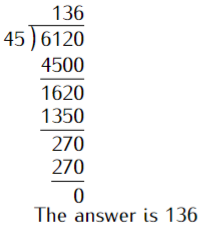
\includegraphics{images/Operations_Ex2.png}

}

\caption{Example 2}

\end{figure}%

\end{tcolorbox}

\begin{tcolorbox}[enhanced jigsaw, left=2mm, colframe=quarto-callout-note-color-frame, toptitle=1mm, opacitybacktitle=0.6, rightrule=.15mm, colbacktitle=quarto-callout-note-color!10!white, colback=white, arc=.35mm, breakable, leftrule=.75mm, bottomtitle=1mm, bottomrule=.15mm, title=\textcolor{quarto-callout-note-color}{\faInfo}\hspace{0.5em}{Example 3}, titlerule=0mm, coltitle=black, toprule=.15mm, opacityback=0]

The Amos family borrows \$ 20,880 to purchase a new car at a special 0\%
interest rate. The car dealer allows them 5 years to pay back the amount
they borrow and requires equal monthly payments. How much are their
monthly payments? \((2mks)\)

\end{tcolorbox}

\begin{tcolorbox}[enhanced jigsaw, left=2mm, colframe=quarto-callout-caution-color-frame, toptitle=1mm, opacitybacktitle=0.6, rightrule=.15mm, colbacktitle=quarto-callout-caution-color!10!white, colback=white, arc=.35mm, breakable, leftrule=.75mm, bottomtitle=1mm, bottomrule=.15mm, title=\textcolor{quarto-callout-caution-color}{\faFire}\hspace{0.5em}{Solution}, titlerule=0mm, coltitle=black, toprule=.15mm, opacityback=0]

Since there are 12 months in each year, they must make a total of
\(5\times12 = 60\), payments on the loan. Dividing \$ 20,880 by 60 will
result in the monthly payment:

\begin{figure}[H]

{\centering 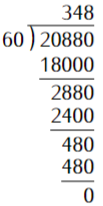
\includegraphics{images/Operations_Ex3.png}

}

\caption{Example 3}

\end{figure}%

The Amos' monthly payment will be \$ 348.

\end{tcolorbox}

\begin{tcolorbox}[enhanced jigsaw, left=2mm, colframe=quarto-callout-note-color-frame, toptitle=1mm, opacitybacktitle=0.6, rightrule=.15mm, colbacktitle=quarto-callout-note-color!10!white, colback=white, arc=.35mm, breakable, leftrule=.75mm, bottomtitle=1mm, bottomrule=.15mm, title=\textcolor{quarto-callout-note-color}{\faInfo}\hspace{0.5em}{Problems to solve}, titlerule=0mm, coltitle=black, toprule=.15mm, opacityback=0]

\begin{enumerate}
\def\labelenumi{\arabic{enumi}.}
\item
  A bus charges \(Ksh.~ 150\) as fare from Embu to Meru. It carries a
  capacity of 18 passengers. However, it can carry 5 more passengers but
  will have to pay a penalty of \(Ksh.~100\) at each of the 8 police
  checkpoints it passes through. The distance between the two towns is
  \(91 ~km\) and the cost of petrol is \(Ksh.~ 102\) per litre. If the
  bus uses 1 litre for every \(7~ km\), calculate;

  a) How much is gained if the bus does not overload? \((4mks)\)

  b) How much is lost if the bus overloads? \((4mks)\)
\item
  A vegetable vendor had 1,652 cabbages. He sold 835 cabbages on the
  first day and 326 cabbages on the second day. He added 413 cabbages to
  the remaining stock on the third day.

  a) How many cabbages did he have at the end? \((3mks)\)

  b) If he sold all the cabbages at an average cost of \(Ksh.~ 15\), how
  much money did he collect? \((1mk)\)
\item
  Perform the following divisions: \((6mks)\)

  a) \(2,668\div58\)

  b) \(867,594 \div 2,317\)

  c) \(0.0021\div 14\)
\item
  A bookshop had \(29,424\) exercise books which were packed in cartons.
  each carton contained \(24\) exercise books. The mass of an empty
  carton was 2 Kg and 11 Kg when full.

  a) How many cartons were there? \((1mk)\)

  b) What was the total mass of empty cartons? \((2mks)\)

  c) What was the total mass of the books alone? \((2mks)\)
\item
  The average mass of students in a class of 45 was 46 Kg at the
  beginning of the year. At the end of the that year, they had each
  gained 4 Kg. Calculate:

  a) Their total mass of the students at the end of the year. \((2mks)\)

  b) The difference between their total mass at the beginning and at the
  end of the year. \((2mks)\)
\item
  A matatu had 23 passengers at the beginning of the journey. Twelve
  passengers alighted at the first stop while 9 boarded. Six of those
  who boarded at the first stop alighted at the second stop and 12 got
  in. The matatu did not stop again up to the final destination. The
  charges from the starting point were Ksh. 50 up to the first stop,
  Ksh. 70 up to the second stop, and Ksh. 85 up to the final
  destination.

  a) How many passengers alighted at the final destination? (3mks)

  b) How many passengers were carried by the matatu through the journey?
  (2mks)

  c) How much money was collected during the trip? (5mks)
\item
  a) State the value of digit 7 after the operations below.

  i) \(3.45 \times 20.54\) (2mks)

  ii) \(0.345 \times 2.054\) (2mks)

  iii) \(34.5\times 0.2054\) (2mks)

  iv) \(0.0345\times 2.054\) (2mks)

  b) states the value of the second digit in the product 675
  \times 44.4. (2mks)
\end{enumerate}

\end{tcolorbox}

\bookmarksetup{startatroot}

\chapter{Chapter 2: Factors}\label{chapter-2-factors}

\bookmarksetup{startatroot}

\chapter*{Factors}\label{factors}
\addcontentsline{toc}{chapter}{Factors}

\markboth{Factors}{Factors}

Factors are all numbers that divide a given number without leaving a
remainder.

\begin{tcolorbox}[enhanced jigsaw, left=2mm, colframe=quarto-callout-note-color-frame, toptitle=1mm, opacitybacktitle=0.6, rightrule=.15mm, colbacktitle=quarto-callout-note-color!10!white, colback=white, arc=.35mm, breakable, leftrule=.75mm, bottomtitle=1mm, bottomrule=.15mm, title=\textcolor{quarto-callout-note-color}{\faInfo}\hspace{0.5em}{Example of Factors}, titlerule=0mm, coltitle=black, toprule=.15mm, opacityback=0]

\begin{figure}[H]

{\centering 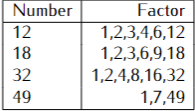
\includegraphics{images/Factor_Table.png}

}

\caption{Example}

\end{figure}%

\end{tcolorbox}

\section{Solved examples}\label{solved-examples-3}

\begin{tcolorbox}[enhanced jigsaw, left=2mm, colframe=quarto-callout-note-color-frame, toptitle=1mm, opacitybacktitle=0.6, rightrule=.15mm, colbacktitle=quarto-callout-note-color!10!white, colback=white, arc=.35mm, breakable, leftrule=.75mm, bottomtitle=1mm, bottomrule=.15mm, title=\textcolor{quarto-callout-note-color}{\faInfo}\hspace{0.5em}{Example 1}, titlerule=0mm, coltitle=black, toprule=.15mm, opacityback=0]

Express the following numbers in terms of their prime factors

a) 150 \((2mks)\)

b) 196 \((2mks)\)

\end{tcolorbox}

\begin{tcolorbox}[enhanced jigsaw, left=2mm, colframe=quarto-callout-caution-color-frame, toptitle=1mm, opacitybacktitle=0.6, rightrule=.15mm, colbacktitle=quarto-callout-caution-color!10!white, colback=white, arc=.35mm, breakable, leftrule=.75mm, bottomtitle=1mm, bottomrule=.15mm, title=\textcolor{quarto-callout-caution-color}{\faFire}\hspace{0.5em}{Solution}, titlerule=0mm, coltitle=black, toprule=.15mm, opacityback=0]

\begin{figure}[H]

{\centering 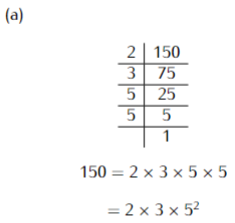
\includegraphics{images/Factor_Ex1_a.png}

}

\caption{Example 1 (a)}

\end{figure}%

\begin{figure}[H]

{\centering 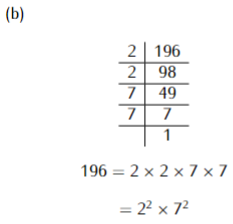
\includegraphics{images/Factor_Ex1_b.png}

}

\caption{Example 1 (b)}

\end{figure}%

\end{tcolorbox}

\begin{tcolorbox}[enhanced jigsaw, left=2mm, colframe=quarto-callout-note-color-frame, toptitle=1mm, opacitybacktitle=0.6, rightrule=.15mm, colbacktitle=quarto-callout-note-color!10!white, colback=white, arc=.35mm, breakable, leftrule=.75mm, bottomtitle=1mm, bottomrule=.15mm, title=\textcolor{quarto-callout-note-color}{\faInfo}\hspace{0.5em}{Problems to solve}, titlerule=0mm, coltitle=black, toprule=.15mm, opacityback=0]

Express the following numbers in terms of their prime factors:

a) 1859 \hspace{11.2cm} \((2mks)\)

b) 105 \hspace{11.4cm} \((2mks)\)

c) 900 \hspace{11.4cm} \((2mks)\)

d) 700 \hspace{11.4cm} \((2mks)\)

e) 5929 \hspace{11.4cm} \((2mks)\)

f) 1078 \hspace{11.4cm} \((2mks)\)

g) 2057 \hspace{11.4cm} \((2mks)\)

h) 1386 \hspace{11.4cm} \((2mks)\)

i) 1573 \hspace{11.4cm} \((2mks)\)

j) 993 \hspace{11.4cm} \((2mks)\)

\end{tcolorbox}

\bookmarksetup{startatroot}

\chapter{Chapter Three: Divisibility
Test}\label{chapter-three-divisibility-test}

\bookmarksetup{startatroot}

\chapter*{Divisibility Test}\label{divisibility-test}
\addcontentsline{toc}{chapter}{Divisibility Test}

\markboth{Divisibility Test}{Divisibility Test}

\section{Divisibility Test for 2, 3, 4, 5, 6, 8, 10, and
11}\label{divisibility-test-for-2-3-4-5-6-8-10-and-11}

\textbf{Divisibility test for 2}

A number is divisible by \textbf{2} if its last digit is \textbf{even or
zero} . e.g., 12, 10, and 72

\textbf{Divisibility test for 3}

A number is divisible by \textbf{3} if the sum of its digits is
divisible by \textbf{3}.

\begin{tcolorbox}[enhanced jigsaw, left=2mm, colframe=quarto-callout-note-color-frame, toptitle=1mm, opacitybacktitle=0.6, rightrule=.15mm, colbacktitle=quarto-callout-note-color!10!white, colback=white, arc=.35mm, breakable, leftrule=.75mm, bottomtitle=1mm, bottomrule=.15mm, title=\textcolor{quarto-callout-note-color}{\faInfo}\hspace{0.5em}{Example}, titlerule=0mm, coltitle=black, toprule=.15mm, opacityback=0]

\(1,275\) is divisible by 3 because the sum of the digit is a multiple
of 3 that is:

\((1+2+7+5=15)=\frac{15}{3}=5\)

\end{tcolorbox}

\textbf{Divisibility test for 4}

A number is divisible by \textbf{4} if its last two digits are both zero
or form a number which is divisible by 4.

\begin{tcolorbox}[enhanced jigsaw, left=2mm, colframe=quarto-callout-note-color-frame, toptitle=1mm, opacitybacktitle=0.6, rightrule=.15mm, colbacktitle=quarto-callout-note-color!10!white, colback=white, arc=.35mm, breakable, leftrule=.75mm, bottomtitle=1mm, bottomrule=.15mm, title=\textcolor{quarto-callout-note-color}{\faInfo}\hspace{0.5em}{Example}, titlerule=0mm, coltitle=black, toprule=.15mm, opacityback=0]

\(1,144\) is divisible by 4 because its last two digits are divisible by
4 to give 11

\end{tcolorbox}

\textbf{Divisibility test for 5}

A number is divisible by 5 if its last digit is zero or 5. e.g 55, 60,
105

\textbf{Divisibility test for 6}

A number is divisible by 6 if it is divisible by both 2 and 3

\textbf{Divisibility test for 8}

A number is divisible by 8 if the number formed by its last 3 digits is
divisible by 8.

\textbf{Divisibility test for 9}

A number is divisible by 9 if the sum of its digits is divisible by 9

\textbf{Divisibility test for 10}

A number is divisible by 10 if the last digit is zero.

\textbf{Divisibility test for 11}

A number is divisible by 11 if the sum of its \textbf{1st, 3rd, 5th,
7th, 9th}, etc. digits and the sum of the 2nd, 4th, 6th, 8th, etc.
digits are equal or differ by 11 or a multiple of 11.

\begin{tcolorbox}[enhanced jigsaw, left=2mm, colframe=quarto-callout-note-color-frame, toptitle=1mm, opacitybacktitle=0.6, rightrule=.15mm, colbacktitle=quarto-callout-note-color!10!white, colback=white, arc=.35mm, breakable, leftrule=.75mm, bottomtitle=1mm, bottomrule=.15mm, title=\textcolor{quarto-callout-note-color}{\faInfo}\hspace{0.5em}{Problems to solve}, titlerule=0mm, coltitle=black, toprule=.15mm, opacityback=0]

\begin{enumerate}
\def\labelenumi{\arabic{enumi}.}
\item
  In each of the following numbers without doing actual division,
  determine whether the first number is divisible by the second number:
  \hspace{8.8 cm} \((5mks)\)

  a) 3409122; 6

  b) 17218; 6

  c) 11309634; ,8

  d) 515712; , 8

  e) 3501804; , 4
\item
  Which of the following numbers has 9 as a factor? \hspace{6cm}
  \((2mks)\)

  a) 394683

  b) 1872546

  c) 5172354
\item
  a) Which are the smallest numbers that can be added to the following
  numbers to make them divisible by 11? \hspace{10.8cm} \((4mks)\)

  i) 5,234

  ii) 36,541

  iii) 96,287

  iv) 27,992

  b) Which are the smallest numbers that can be subtracted from the
  following numbers to make them divisible by 11? \hspace{10cm}
  \((2mks)\)

  i) 96,287 ii) 24,535
\item
  Test whether 712,038 is divisible by: \hspace{8.5cm} \((3mks)\)

  i) 2

  ii) 3

  iii) 4
\end{enumerate}

\end{tcolorbox}

\bookmarksetup{startatroot}

\chapter{Chapter 4: G.C.D and L.C.M}\label{chapter-4-g.c.d-and-l.c.m}

\bookmarksetup{startatroot}

\chapter*{Greatest Common Divisor and Least Common
Divisor}\label{greatest-common-divisor-and-least-common-divisor}
\addcontentsline{toc}{chapter}{Greatest Common Divisor and Least Common
Divisor}

\markboth{Greatest Common Divisor and Least Common Divisor}{Greatest
Common Divisor and Least Common Divisor}

\section{Greatest Common Divisor
(GCD)}\label{greatest-common-divisor-gcd}

GCD is also called the Highest Common Factor (HCF) or Greatest Common
Factor (GCF). To find the GCF of two numbers you write down their prime
factors, then select the common factors and obtain their product.

\begin{tcolorbox}[enhanced jigsaw, left=2mm, colframe=quarto-callout-note-color-frame, toptitle=1mm, opacitybacktitle=0.6, rightrule=.15mm, colbacktitle=quarto-callout-note-color!10!white, colback=white, arc=.35mm, breakable, leftrule=.75mm, bottomtitle=1mm, bottomrule=.15mm, title=\textcolor{quarto-callout-note-color}{\faInfo}\hspace{0.5em}{Solved Example}, titlerule=0mm, coltitle=black, toprule=.15mm, opacityback=0]

Find the HCF of 36 and 64. \hspace{10.5cm} \((3mks)\)

\end{tcolorbox}

\begin{tcolorbox}[enhanced jigsaw, left=2mm, colframe=quarto-callout-caution-color-frame, toptitle=1mm, opacitybacktitle=0.6, rightrule=.15mm, colbacktitle=quarto-callout-caution-color!10!white, colback=white, arc=.35mm, breakable, leftrule=.75mm, bottomtitle=1mm, bottomrule=.15mm, title=\textcolor{quarto-callout-caution-color}{\faFire}\hspace{0.5em}{Solution}, titlerule=0mm, coltitle=black, toprule=.15mm, opacityback=0]

\begin{figure}[H]

{\centering 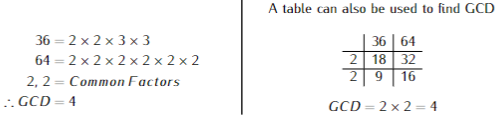
\includegraphics{images/GCD_Ex1.png}

}

\caption{GCD Example}

\end{figure}%

\end{tcolorbox}

\section{Least Common Multiple (LCM)}\label{least-common-multiple-lcm}

The least common multiple, or smallest common multiple, or lowest common
multiple of two integers is the smallest positive integer that is
divisible by the two integers.

\section{Solved Examples}\label{solved-examples-4}

\begin{tcolorbox}[enhanced jigsaw, left=2mm, colframe=quarto-callout-note-color-frame, toptitle=1mm, opacitybacktitle=0.6, rightrule=.15mm, colbacktitle=quarto-callout-note-color!10!white, colback=white, arc=.35mm, breakable, leftrule=.75mm, bottomtitle=1mm, bottomrule=.15mm, title=\textcolor{quarto-callout-note-color}{\faInfo}\hspace{0.5em}{Example 1}, titlerule=0mm, coltitle=black, toprule=.15mm, opacityback=0]

What is the LCM of 18, 24 and 36? \hspace{9.5cm} \((2mks)\)

\end{tcolorbox}

\begin{tcolorbox}[enhanced jigsaw, left=2mm, colframe=quarto-callout-caution-color-frame, toptitle=1mm, opacitybacktitle=0.6, rightrule=.15mm, colbacktitle=quarto-callout-caution-color!10!white, colback=white, arc=.35mm, breakable, leftrule=.75mm, bottomtitle=1mm, bottomrule=.15mm, title=\textcolor{quarto-callout-caution-color}{\faFire}\hspace{0.5em}{Solution}, titlerule=0mm, coltitle=black, toprule=.15mm, opacityback=0]

\begin{figure}[H]

{\centering 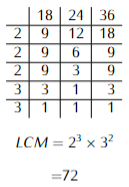
\includegraphics{images/GCD_LCM_Ex1.png}

}

\caption{Example 1}

\end{figure}%

\end{tcolorbox}

\begin{tcolorbox}[enhanced jigsaw, left=2mm, colframe=quarto-callout-note-color-frame, toptitle=1mm, opacitybacktitle=0.6, rightrule=.15mm, colbacktitle=quarto-callout-note-color!10!white, colback=white, arc=.35mm, breakable, leftrule=.75mm, bottomtitle=1mm, bottomrule=.15mm, title=\textcolor{quarto-callout-note-color}{\faInfo}\hspace{0.5em}{Example 2}, titlerule=0mm, coltitle=black, toprule=.15mm, opacityback=0]

The G.C.D of two numbers is 12 and their L.C.M is 240. If one of the
numbers is 60, find the other number \hspace{14cm} \((3mks)\)

\end{tcolorbox}

\begin{tcolorbox}[enhanced jigsaw, left=2mm, colframe=quarto-callout-caution-color-frame, toptitle=1mm, opacitybacktitle=0.6, rightrule=.15mm, colbacktitle=quarto-callout-caution-color!10!white, colback=white, arc=.35mm, breakable, leftrule=.75mm, bottomtitle=1mm, bottomrule=.15mm, title=\textcolor{quarto-callout-caution-color}{\faFire}\hspace{0.5em}{Solution}, titlerule=0mm, coltitle=black, toprule=.15mm, opacityback=0]

\begin{figure}[H]

{\centering 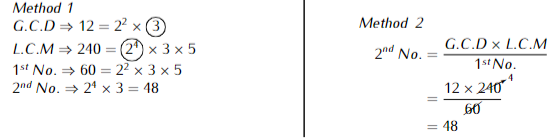
\includegraphics{images/GCD_LCM_Ex2.png}

}

\caption{Example 2}

\end{figure}%

\end{tcolorbox}

\begin{tcolorbox}[enhanced jigsaw, left=2mm, colframe=quarto-callout-note-color-frame, toptitle=1mm, opacitybacktitle=0.6, rightrule=.15mm, colbacktitle=quarto-callout-note-color!10!white, colback=white, arc=.35mm, breakable, leftrule=.75mm, bottomtitle=1mm, bottomrule=.15mm, title=\textcolor{quarto-callout-note-color}{\faInfo}\hspace{0.5em}{Problems to solve}, titlerule=0mm, coltitle=black, toprule=.15mm, opacityback=0]

\begin{enumerate}
\def\labelenumi{\arabic{enumi}.}
\item
  The GCD of three numbers is 30 and their LCM is 900. Two of the
  numbers are 60 and 150. Find the other possible numbers.
  \hspace{8.7cm} \((3mks)\)
\item
  the least common multiple of two numbers is 60 and one of the numbers
  is 7 less than the other. What are the numbers? \hspace{10.3cm}
  \((3mks)\)
\item
  The L.C.M of two numbers is 120 and their G.C.F is 6. One of the
  numbers is 30, what is the other number? \hspace{11.8cm} \((3mks)\)
\item
  Three bells rang at intervals of 9minutes, 15 minutes and 21minutes.
  The bells will ring together at 11.00 p.m.Find the time the bells had
  last rang together. \hspace{5cm} \((3mks)\)
\item
  a) The difference between the GCD and the LCM of 36 and
  54.\hspace{4cm} \((2mks)\)

  b) If three numbers 36, 54 and have a GCD of 6 and LCM of 216. Find
  the least value of the third number. \hspace{11.1cm} \((2mks)\)
\item
  The GCD and LCM of three numbers are 3 and 1,008 respectively. If two
  of the numbers are 48 and 72, find the least possible value of the
  third number.\hspace{5cm} \((3mks)\)
\item
  Three alarms ring at intervals of 40 minutes, 45 minutes, and 60
  minutes. If they ring simultaneously at 6:30 a.m., at what time will
  they next ring together? \hspace{3.9cm} \((3mks)\)
\item
  Four traffic light signals are programmed at intervals of 40 seconds,
  50 seconds, 60 seconds, and 75 seconds. What is the earliest they will
  give out light signals simultaneously if the last time they did this
  was at 8:15 a.m.? \hspace{8.5cm} \((3mks)\)
\item
  A number n is such that when it is divided by 27, 30, or 45, the
  remainder is 5. Find the smallest possible value of n.~\hspace{11cm}
  \((3mks)\)
\item
  Find the greatest number which divides 181 and 170 leaving a remainder
  of 5. \hspace{1.7cm} \((3mks)\)
\item
  A square room is covered by a number of whole rectangular slabs of
  sides 60cm by 42 cm. Calculate the least possible area of the room in
  square meters. \hspace{4cm} \((3mks)\)
\item
  Three metal rods of lengths 234cm, 270cm, and 324cm were cut into
  shorter pieces all of the same length to make window grills. Calculate
  the length of the longest piece that can be cut from each of the rods
  and hence the total number of pieces that can be obtained from the
  rods. \hspace{14.2cm} \((4mks)\)
\item
  The GCD of two numbers is 7 and their LCM is 140. If one of the
  numbers is 20, find the other number. \hspace{12.8cm} \((2mks)\)
\item
  The GCD and LCM of three numbers are 84 and 7056 respectively. If two
  of the numbers are 168 and 336, find the least possible value of the
  third number.\hspace{5cm} \((3mks)\)
\item
  A fruit juice dealer sells the juice in a packet of 300ml, 500ml, and
  750ml. Find the size of the smallest container that can fill each of
  the packets and leave a remainder of 200ml.\hspace{0.6cm} \((3mks)\)
\item
  Mr.~Ombogo the principal of Chiga secondary would wish to cover the
  floor of the new administration block using the square tiles. The
  floor is a rectangle of sides 12.8m by 8.4m. Find the area of each of
  the largest tiles which can be used to fit exactly without breaking.
  \hspace{14.2cm} \((3mks)\)
\item
  Three numbers, 1400, 1960, and n have a G.C.D and L.C.M of 70 and
  \(2^2\times 5^2\times 7^2 \times 11\) respectively. Find the least
  possible value of n.~\hspace{8.8cm} \((3mks)\)
\item
  a) Express 48 and 60 as a product of their prime factors.
  \hspace{11cm} \((3mks)\)

  b) A room of sides 48m and 60m is to be decorated using square tiles
  side XM. Find the greatest area of the tile. \hspace{9.2cm} \((2mks)\)
\item
  Three similar pieces of timber of length 240cm, 320cm, and 380cm are
  cut into equal pieces. Find the largest possible area of a square that
  can be made from any of the three pieces. \hspace{14.2cm} \((3mks)\)
\end{enumerate}

\end{tcolorbox}

\bookmarksetup{startatroot}

\chapter{Chapter 5: Integers}\label{chapter-5-integers}

\bookmarksetup{startatroot}

\chapter*{Integers}\label{integers}
\addcontentsline{toc}{chapter}{Integers}

\markboth{Integers}{Integers}

\section{The Number Line}\label{the-number-line}

Integers are positive whole numbers, negative whole numbers, and zero.
Integers are usually represented on the number line at equal intervals,
as shown in the figure below, where each interval is equal to one unit.

\begin{figure}

\centering{

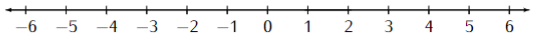
\includegraphics{images/Number_Line.png}

}

\caption{\label{fig-numberline}Number Line}

\end{figure}%

Important properties to note while working with integers:

\begin{quote}
\textbf{Multiplication and division properties of integers}

\begin{itemize}
\item
  \((+)\times(-) = -\)
\item
  \((-) \times (+) = -\)
\item
  \((-) \times (-) = +\)
\item
  \((+) \times(+) = +\)
\item
  \((+)\div(-) = -\)
\item
  \((-)\div(+) = -\)
\item
  \((-)\div(-) = +\)
\end{itemize}
\end{quote}

\section{Solved Examples}\label{solved-examples-5}

\begin{tcolorbox}[enhanced jigsaw, left=2mm, colframe=quarto-callout-note-color-frame, toptitle=1mm, opacitybacktitle=0.6, rightrule=.15mm, colbacktitle=quarto-callout-note-color!10!white, colback=white, arc=.35mm, breakable, leftrule=.75mm, bottomtitle=1mm, bottomrule=.15mm, title=\textcolor{quarto-callout-note-color}{\faInfo}\hspace{0.5em}{Example 1}, titlerule=0mm, coltitle=black, toprule=.15mm, opacityback=0]

Show how the following additions can be done using a number line and
give the results: \((6mks)\)

a) \((-4)+(+6)\)

b) \((-5)+(+4)\)

c) \((+2)+(-6)\)

\end{tcolorbox}

\begin{tcolorbox}[enhanced jigsaw, left=2mm, colframe=quarto-callout-caution-color-frame, toptitle=1mm, opacitybacktitle=0.6, rightrule=.15mm, colbacktitle=quarto-callout-caution-color!10!white, colback=white, arc=.35mm, breakable, leftrule=.75mm, bottomtitle=1mm, bottomrule=.15mm, title=\textcolor{quarto-callout-caution-color}{\faFire}\hspace{0.5em}{Solution}, titlerule=0mm, coltitle=black, toprule=.15mm, opacityback=0]

\begin{figure}[H]

{\centering 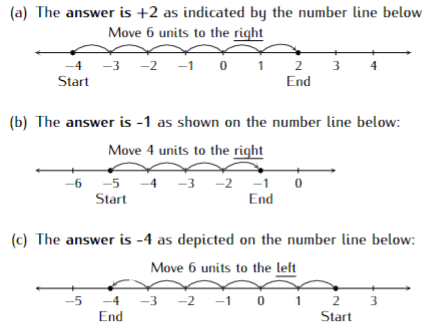
\includegraphics{images/Number_Line_ex1.png}

}

\caption{Example 1}

\end{figure}%

\end{tcolorbox}

\begin{tcolorbox}[enhanced jigsaw, left=2mm, colframe=quarto-callout-note-color-frame, toptitle=1mm, opacitybacktitle=0.6, rightrule=.15mm, colbacktitle=quarto-callout-note-color!10!white, colback=white, arc=.35mm, breakable, leftrule=.75mm, bottomtitle=1mm, bottomrule=.15mm, title=\textcolor{quarto-callout-note-color}{\faInfo}\hspace{0.5em}{Example 2}, titlerule=0mm, coltitle=black, toprule=.15mm, opacityback=0]

Fill in the boxes in numbers below:\hspace{10cm} \((3mks)\)

i) \((-3)+\square=+10\)

ii) \(\square +(-7)=-11\)

iii) \((-4)+(-2)+\square =+3\)

\end{tcolorbox}

\begin{tcolorbox}[enhanced jigsaw, left=2mm, colframe=quarto-callout-caution-color-frame, toptitle=1mm, opacitybacktitle=0.6, rightrule=.15mm, colbacktitle=quarto-callout-caution-color!10!white, colback=white, arc=.35mm, breakable, leftrule=.75mm, bottomtitle=1mm, bottomrule=.15mm, title=\textcolor{quarto-callout-caution-color}{\faFire}\hspace{0.5em}{Solution}, titlerule=0mm, coltitle=black, toprule=.15mm, opacityback=0]

i) \(\square=+10+3=13\)

ii) \(\square=-11+7=-4\)

iii) \(\square-4-2=+3 \Rightarrow \square=3+6=+9\)

\end{tcolorbox}

\begin{tcolorbox}[enhanced jigsaw, left=2mm, colframe=quarto-callout-note-color-frame, toptitle=1mm, opacitybacktitle=0.6, rightrule=.15mm, colbacktitle=quarto-callout-note-color!10!white, colback=white, arc=.35mm, breakable, leftrule=.75mm, bottomtitle=1mm, bottomrule=.15mm, title=\textcolor{quarto-callout-note-color}{\faInfo}\hspace{0.5em}{Example 3}, titlerule=0mm, coltitle=black, toprule=.15mm, opacityback=0]

Without using a calculator evaluate, \hspace{10cm} \((3mks)\)

\[ 
\frac{-2(4+3)-12\div3 +2}{-6\times-3+-2\times4}
\]

\end{tcolorbox}

\begin{tcolorbox}[enhanced jigsaw, left=2mm, colframe=quarto-callout-caution-color-frame, toptitle=1mm, opacitybacktitle=0.6, rightrule=.15mm, colbacktitle=quarto-callout-caution-color!10!white, colback=white, arc=.35mm, breakable, leftrule=.75mm, bottomtitle=1mm, bottomrule=.15mm, title=\textcolor{quarto-callout-caution-color}{\faFire}\hspace{0.5em}{Solution}, titlerule=0mm, coltitle=black, toprule=.15mm, opacityback=0]

\textbf{Using BODMAS}

\begin{equation}
\begin{split}
\text{Numerator} & = 2(4+3) - 12 \div 3 + 2 \\
& = 14 - 4 + 2 \\
& = 12 \\
\text{Denominator} & = -6 \times -3 + -2 \times 4 \\
& = 18 + -8 \\
& = 10 \\
\therefore & = \frac{12}{10} = \frac{6}{5} = 1 \frac{1}{5} \\
\end{split}
\end{equation}

\end{tcolorbox}

\begin{tcolorbox}[enhanced jigsaw, left=2mm, colframe=quarto-callout-note-color-frame, toptitle=1mm, opacitybacktitle=0.6, rightrule=.15mm, colbacktitle=quarto-callout-note-color!10!white, colback=white, arc=.35mm, breakable, leftrule=.75mm, bottomtitle=1mm, bottomrule=.15mm, title=\textcolor{quarto-callout-note-color}{\faInfo}\hspace{0.5em}{Problem to Solve}, titlerule=0mm, coltitle=black, toprule=.15mm, opacityback=0]

\begin{enumerate}
\def\labelenumi{\arabic{enumi}.}
\tightlist
\item
  Without using a calculator, evaluate \hspace{9.65cm} \((3mks)\).
\end{enumerate}

\[\frac{(-8+(-5)\times(-8)-(-6)}{-3+(-8)\div2\times4} \]

\begin{enumerate}
\def\labelenumi{\arabic{enumi}.}
\setcounter{enumi}{1}
\item
  Orengo bought 1848 Mangoes on a Wednesday and sold 650 of them on the
  same day. On Thursday, he sold 180 more Mangoes than on Wednesday. On
  Friday he bought 460 more Mangoes. Later that day, he sold all the
  Mangoes he had at a price of Ksh. 10 each. How much money did he make?
  \hspace{12cm} \((3mks)\)
\item
  Evaluate: \hspace{10.3cm} \((3mks)\)
\end{enumerate}

\[\frac{-12\div(-3)\times4-(-20)}{-6\times6\div+(-6)} \]

\begin{enumerate}
\def\labelenumi{\arabic{enumi}.}
\setcounter{enumi}{3}
\tightlist
\item
  Without using tables or a calculator, evaluate \hspace{6.85cm}
  \((3mks)\)
\end{enumerate}

\[ \frac{(-2)\times 7+(-4) \div (-3)}{3 \times (-2)+5\times (-4)}\]

\begin{enumerate}
\def\labelenumi{\arabic{enumi}.}
\setcounter{enumi}{4}
\tightlist
\item
  Without using a calculator, evaluate \hspace{10.7cm} \((3mks)\)\\
\end{enumerate}

\[\frac{-5(-23+41)-(-10)}{-3+(-8)\div2\times4}\]

\begin{enumerate}
\def\labelenumi{\arabic{enumi}.}
\setcounter{enumi}{5}
\item
  Show how the following additions can be done using a number line and
  give the results:

  a) \((-8)+(+5)\) \hspace{12cm} \((2mks)\)

  b) \((-7)+(+2)\) \hspace{12cm} \((2mks)\)

  c) \((-6)+(+4)+(+2)\) \hspace{10.95cm} \((2mks)\)
\end{enumerate}

\end{tcolorbox}

\bookmarksetup{startatroot}

\chapter{Chapter 6: Fractions}\label{chapter-6-fractions}

\bookmarksetup{startatroot}

\chapter*{Fractions}\label{fractions}
\addcontentsline{toc}{chapter}{Fractions}

\markboth{Fractions}{Fractions}

A fraction is written in the form of \(\frac{x}{y}\) where \(x\) and
\(y\) are numbers and \(y\neq0\). The number on the upper side \((x)\)
is called numerator and the number on the lower side \((y)\) is called
Denominator.

There are three types of fractions:

\begin{itemize}
\item
  \textbf{Proper fractions:} These are fractions whose numerator is
  smaller than the denominator.
\item
  \textbf{Improper fractions:} These are the fractions whose numerator
  is bigger than the denominator
\item
  \textbf{Mixed fractions:} They are fractions written in the form of an
  integer and a proper fraction.
\end{itemize}

\section{Solved Examples}\label{solved-examples-6}

\begin{tcolorbox}[enhanced jigsaw, left=2mm, colframe=quarto-callout-note-color-frame, toptitle=1mm, opacitybacktitle=0.6, rightrule=.15mm, colbacktitle=quarto-callout-note-color!10!white, colback=white, arc=.35mm, breakable, leftrule=.75mm, bottomtitle=1mm, bottomrule=.15mm, title=\textcolor{quarto-callout-note-color}{\faInfo}\hspace{0.5em}{Example 1}, titlerule=0mm, coltitle=black, toprule=.15mm, opacityback=0]

Evaluate: \hspace{9cm} \((3mks)\)

\[
\frac{8\times \frac{1}{3} \, of\, 9\div 2-\frac{2}{3}\, of \,144 \div 12+2 \times 3}{\frac{3}{4}\, of \,36 \div 3-4\div \frac{2}{5} \,of \,10+3 \times (-2)}  
\]

\end{tcolorbox}

\begin{tcolorbox}[enhanced jigsaw, left=2mm, colframe=quarto-callout-caution-color-frame, toptitle=1mm, opacitybacktitle=0.6, rightrule=.15mm, colbacktitle=quarto-callout-caution-color!10!white, colback=white, arc=.35mm, breakable, leftrule=.75mm, bottomtitle=1mm, bottomrule=.15mm, title=\textcolor{quarto-callout-caution-color}{\faFire}\hspace{0.5em}{Solution}, titlerule=0mm, coltitle=black, toprule=.15mm, opacityback=0]

\textbf{Using BODMAS}

\begin{equation}
\begin{split}
Numerator: 
&=8\times \left(\frac{1}{3}\times9\right)\div 2-\left (\frac{2}{3}\times144\right)\div12+2\times3\\
&=8\times(3\div 2)-(96\div 12)+2 \times 3\\  
&=\left (8 \times \frac{3}{2}\right)-8+(2\times 3)\\
&=12-8+6\\
&=10\\
\end{split}
\end{equation}

\begin{equation}
\begin{split}
Denominator:
&=\left( \frac{3}{4}\times36\right)\div 3-4\div\left (\frac{2}{5}\times10\right)+3\times(-2)\\
&=(27\div3)-(4\div4)+3\times-2\\
&=9-1+(3\times-2)\\
&=9-1-6\\
&=2\\
\therefore \frac{10}{2} &=5
\end{split}
\end{equation}

\end{tcolorbox}

\begin{tcolorbox}[enhanced jigsaw, left=2mm, colframe=quarto-callout-note-color-frame, toptitle=1mm, opacitybacktitle=0.6, rightrule=.15mm, colbacktitle=quarto-callout-note-color!10!white, colback=white, arc=.35mm, breakable, leftrule=.75mm, bottomtitle=1mm, bottomrule=.15mm, title=\textcolor{quarto-callout-note-color}{\faInfo}\hspace{0.5em}{Example 2}, titlerule=0mm, coltitle=black, toprule=.15mm, opacityback=0]

James withdrew some money from a bank. He spent \(\frac{3}{8}\) of the
money to pay for his son's school fees and \(\frac{2}{5}\) to pay for
his daughter's school fees. If he remained with \(Ksh. 12, 330\),
calculate the amount of money he paid for his daughter's school fees.
\hspace{9.7cm} \((3mks)\)

\end{tcolorbox}

\begin{tcolorbox}[enhanced jigsaw, left=2mm, colframe=quarto-callout-caution-color-frame, toptitle=1mm, opacitybacktitle=0.6, rightrule=.15mm, colbacktitle=quarto-callout-caution-color!10!white, colback=white, arc=.35mm, breakable, leftrule=.75mm, bottomtitle=1mm, bottomrule=.15mm, title=\textcolor{quarto-callout-caution-color}{\faFire}\hspace{0.5em}{Solution}, titlerule=0mm, coltitle=black, toprule=.15mm, opacityback=0]

\begin{equation}
\begin{split}
Let\,his\, money\, be \,x \\
Son's\,school\, fees &= \frac{3}{8}x \\
Daughter's \,school\, fees&=\frac{2}{5}x \\
Remaining \,fraction&=x-\left( \frac{3}{8}x+\frac{2}{5}x\right)\\ x-\left ( \frac{31}{40}x\right) &=\frac{9}{40}x\\ 
\end{split}
\end{equation}

\begin{equation}
\begin{split}
\frac{9}{40}x &= 12330 \\ 
\text{Multiply both sides by } \frac{40}{9} & \\
\therefore x &= 12330 \times \frac{40}{9} \\ 
x &= 54800 \\ 
\text{Daughter's school fees} &= \left( \frac{2}{5} \right) \times 54800 \\ 
&= \text{Ksh. } 21,920 
\end{split}
\end{equation}

\end{tcolorbox}

\begin{tcolorbox}[enhanced jigsaw, left=2mm, colframe=quarto-callout-note-color-frame, toptitle=1mm, opacitybacktitle=0.6, rightrule=.15mm, colbacktitle=quarto-callout-note-color!10!white, colback=white, arc=.35mm, breakable, leftrule=.75mm, bottomtitle=1mm, bottomrule=.15mm, title=\textcolor{quarto-callout-note-color}{\faInfo}\hspace{0.5em}{Example 3}, titlerule=0mm, coltitle=black, toprule=.15mm, opacityback=0]

In a certain church, there are 200 more women than men. One-third of the
men and two-fifths of the women are elderly people. If there are 300
elderly people in the meeting, find out how many young people attend the
church.\hspace{12.1cm} \((3mks)\)

\end{tcolorbox}

\begin{tcolorbox}[enhanced jigsaw, left=2mm, colframe=quarto-callout-caution-color-frame, toptitle=1mm, opacitybacktitle=0.6, rightrule=.15mm, colbacktitle=quarto-callout-caution-color!10!white, colback=white, arc=.35mm, breakable, leftrule=.75mm, bottomtitle=1mm, bottomrule=.15mm, title=\textcolor{quarto-callout-caution-color}{\faFire}\hspace{0.5em}{Solution}, titlerule=0mm, coltitle=black, toprule=.15mm, opacityback=0]

\begin{equation}
\begin{split}
Let\, \,men&=x\\
women&=x+200\\
Elderly \,people&=300\\
\frac{1}{3}x+\frac{2}{5}(x+200)&=300\\
\frac{1}{3}x+\frac{2}{5}x+80&=300\\ 
\end{split}
\end{equation}

\begin{equation}
\begin{split}
\frac{11}{15}x &= 220 \\
\frac{\cancel{15}}{\cancel{11}} \times \frac{\cancel{11}}{\cancel{15}}x &= \cancelto{20}{220} \times \frac{15}{\cancel{11}} \\
x &= 20 \times 15\\
&= 300 \, \text{men}\\ 
\text{Total number of people:} \\
\text{men + women} &= 300 + 300 + 200\\
&= 800\\
\text{young people} &= 800 - 300\\
&= 500\\
\end{split}
\end{equation}

\end{tcolorbox}

\begin{tcolorbox}[enhanced jigsaw, left=2mm, colframe=quarto-callout-note-color-frame, toptitle=1mm, opacitybacktitle=0.6, rightrule=.15mm, colbacktitle=quarto-callout-note-color!10!white, colback=white, arc=.35mm, breakable, leftrule=.75mm, bottomtitle=1mm, bottomrule=.15mm, title=\textcolor{quarto-callout-note-color}{\faInfo}\hspace{0.5em}{Problems to solve}, titlerule=0mm, coltitle=black, toprule=.15mm, opacityback=0]

\begin{enumerate}
\def\labelenumi{\arabic{enumi}.}
\item
  Three people Karimi, Omondi, and Ali contributed money to start a
  business. Karimi contributed a quarter of the total amount and Omondi
  two-fifths of the remainder. Ali's contribution was one and a half
  times that of Karimi. They borrowed the rest of the money from the
  bank which was \(Ksh.\, 60, 000\) less than Ali's contribution, find
  the total amount required to start the business. \hspace{14.3cm}
  \((4mks)\)
\item
  Three people Gatungo, Martin, and Albert contributed money to purchase
  a flour mill. Gatungo contributed \(\frac{1}{3}\) of the total amount,
  Martin contributed \(\frac{3}{8}\) of the remaining amount and Albert
  contributed the rest of the money. The difference in contribution
  between Martin and Albert was \(Ksh. \,40, 000\). Calculate the price
  of the flour mill. \hspace{6cm} \((3mks)\)
\item
  Agnes paid rent which was \(\frac{1}{10}\) of her net salary. She used
  \(\frac{1}{2}\) of the remaining amount to make a down payment for a
  plot. She gave her mother \(Ksh.\, 2,500\) and did shopping worth
  \(Ksh.\, 7,500\) for herself. She saved the remainder which was
  \(Ksh.\, 12,500\). How much was the down payment that she made?
  \hspace{11.9cm} \((4mks)\)
\item
  King'oo spends one-third of his salary on food, one-quarter on rent,
  three--fifths of the remainder on transport, and saves the rest. If he
  spends \(Ksh. \,1,800\) on transport, find how much money he
  saves.\hspace{13.3cm} \((3mks)\)
\item
  Without using a calculator or mathematical table evaluate:
  \hspace{5.3cm} \((3mks)\)
\end{enumerate}

\[
\frac{2\frac{1}{5}+\frac{2}{3}\,of\,3\frac{3}{4}-4\frac{1}{6}}{1\frac{1}{4}+2\frac{2}{5}\div 1\frac{1}{3}+3\frac{3}{4}}  
\] 6. Without using a calculator, evaluate \hspace{11.5cm} \((3mks)\)

\[
\frac{\frac{3}{4}+1\frac{5}{7}\div \frac{4}{7}\,of\, 2\frac{1}{3}}{\left (1\frac{3}{7}-\frac{5}{8}\right)\times\frac{2}{3}}  
\] 7. Evaluate \hspace{9.5cm} \((3mks)\)

\[
\frac{\frac{3}{5}\,of\,60-2\frac{2}{3}\times1\frac{1}{2}}{5\frac{5}{8}\times1\frac{7}{9}-\frac{5}{4}\,of\,4\frac{4}{5}+2\frac{4}{5}\div\frac{7}{10}} 
\]

\begin{enumerate}
\def\labelenumi{\arabic{enumi}.}
\setcounter{enumi}{7}
\item
  Two boys and a girl shared some money. The younger boy \(\frac{5}{8}\)
  of it. The elder boy got \(\frac{7}{12}\) of the remainder and the
  girl got the rest. Find the percentage share of the younger boy to the
  girl's share. \hspace{13.2cm} \((2mks)\)
\item
  Evaluate without using a calculator. \((3mks)\)
\end{enumerate}

\[
\frac{\left( 2\frac{3}{7}-1\frac{5}{6}\right)\div\frac{5}{6}}{\frac{2}{3}\,of\,2\frac{1}{4}-1\frac{1}{7}}
\]

\begin{enumerate}
\def\labelenumi{\arabic{enumi}.}
\setcounter{enumi}{9}
\tightlist
\item
  Evaluate: \((3mks)\)
\end{enumerate}

\[
\frac{\sqrt[]{\frac{1}{4}}\,of\,3\frac{1}{2}+\frac{3}{2}\left(\frac{5}{2}-\frac{2}{3}\right)}{\frac{3}{4}\,of\,2\frac{1}{2}\div\frac{1}{4}} 
\]

\begin{enumerate}
\def\labelenumi{\arabic{enumi}.}
\setcounter{enumi}{10}
\tightlist
\item
  Without using a calculator, evaluate: \((3mks)\)
\end{enumerate}

\[
\frac{1\frac{4}{5}\,of\,\frac{25}{18}\div1\frac{2}{3}\times24}{2\frac{1}{3}-\frac{1}{4}\,of\,12\div\frac{5}{3}}    
\]

\begin{enumerate}
\def\labelenumi{\arabic{enumi}.}
\setcounter{enumi}{11}
\item
  Evaluate \hspace{12.8cm} \((6mks)\)

  a)
  \[\frac{5\frac{3}{5}\times 1\frac{3}{4}+8\frac{1}{3} \div \frac{5}{9}}{5\frac{1}{6}\times 1\frac{1}{5}}\]

  b)
  \[\frac{8\frac{2}{5}-3\frac{2}{3}\div 1\frac{5}{6}}{1\frac{1}{5}+ 1\frac{1}{3}\times 1\frac{1}{2}}\]
\item
  A man spent \(\frac{1}{9}\) his salary on food and \(\frac{1}{4}\) the
  remainder on electricity and water bills. He paid fees with \(20\%\)
  of his salary and invested \(16\%\) of what was left on business.\\
  After taking a game drive on which he spent \(Ksh. \,2,000\), he saved
  \(Ksh.\,5,350\). Calculate his monthly earnings. \((3mks)\)
\item
  In a mixed secondary school there are 60 more boys than girls. Half of
  the boys and \(\frac{2}{3}\) of the girls are boarders. If there are
  240 boarders, find the total number of students in the school.
  \hspace{14.2cm} \((3mks)\)
\item
  Five members of `SILK', a self-supporting enterprise Jane, Jepchoge,
  Esther, Mama Charo, and Chepkoech were given a certain amount of money
  to share amongst themselves.Jane got \(\frac{3}{8}\) of the total
  amount while Jepchoge got \(\frac{2}{5}\) of the remainder.The
  remaining amount was shared equally among Esther, Mama Charo, and
  Chepkoech each of which received \(Ksh.\, 6,000\);

  a) How much was shared among the five businesswomen? \hspace{4.3cm}
  \((3mks)\)

  b) How much did Jepchoge get? \hspace{8.5cm} \((2mks)\)

  c) Jane, Jepchoge, and Chepkoech invested their money and earned a
  profit of \(Ksh.\, 12,000\). A third of the profit was left to
  maintain the business and the rest was shared according to their
  investments. Find how much each got.\hspace{6.5cm} \((5mks)\)
\end{enumerate}

\end{tcolorbox}

\bookmarksetup{startatroot}

\chapter{Chapter Seven: Decimals, Squares, and Square
Roots}\label{chapter-seven-decimals-squares-and-square-roots}

\bookmarksetup{startatroot}

\chapter*{Decimals, Squares, and Square
Roots}\label{decimals-squares-and-square-roots}
\addcontentsline{toc}{chapter}{Decimals, Squares, and Square Roots}

\markboth{Decimals, Squares, and Square Roots}{Decimals, Squares, and
Square Roots}

\textbf{Decimal fraction} (Decimal), is a fraction whose denominator can
be written as a power of \(10\),
e.g.\(\frac{1}{10},\,\frac{3}{100}, and\,\frac{50}{100}\).

Decimal fractions are usually written in a special way, e.g.,
\(\frac{3}{10}\) written as \(0.3\). The dot in this notation is called
the \textbf{decimal point}. A decimal fraction that represents the sum
of a whole number and a proper fraction is called a \textbf{mixed
decimal}. In division, a decimal fraction in which a digit or a group of
digits repeat continuously without ending is called a \textbf{recurring
decimal} e.g.~\(\frac{5}{11}\)= 0.4545\ldots, in short, we place dots
above the digits that recurs e.g.~0.4545\ldots written as
\(0.\dot{4}\dot{5}\) A number is said to be in \textbf{standard form} if
it is expressed in the form \(A\times 10^n\) where \(1\leq A<10\) and
\(n\) is an integer e.g.~\(0.0065\) is written in standard form as
\(6.5\times 10^{-3}\).

\textbf{Squares} of numbers are tabulated and can be read from the table
of squares which gives only approximate values of the square to four
figures.

\textbf{Square root} of a number can be obtained using the factorization
method or tables of square roots in a mathematical table.

\section{Solved Exambles}\label{solved-exambles}

\begin{tcolorbox}[enhanced jigsaw, left=2mm, colframe=quarto-callout-note-color-frame, toptitle=1mm, opacitybacktitle=0.6, rightrule=.15mm, colbacktitle=quarto-callout-note-color!10!white, colback=white, arc=.35mm, breakable, leftrule=.75mm, bottomtitle=1mm, bottomrule=.15mm, title=\textcolor{quarto-callout-note-color}{\faInfo}\hspace{0.5em}{Example 1}, titlerule=0mm, coltitle=black, toprule=.15mm, opacityback=0]

Without using table or calculators, evaluate:

\[
\sqrt[]{\frac{0.0032+0.0608}{1.44\times 0.4}} \hspace{12cm} (3mks)
\]

\end{tcolorbox}

\begin{tcolorbox}[enhanced jigsaw, left=2mm, colframe=quarto-callout-caution-color-frame, toptitle=1mm, opacitybacktitle=0.6, rightrule=.15mm, colbacktitle=quarto-callout-caution-color!10!white, colback=white, arc=.35mm, breakable, leftrule=.75mm, bottomtitle=1mm, bottomrule=.15mm, title=\textcolor{quarto-callout-caution-color}{\faFire}\hspace{0.5em}{Solution}, titlerule=0mm, coltitle=black, toprule=.15mm, opacityback=0]

\begin{equation}
\begin{split}
0.0032 + 0.0608 & = 0.0640 \\
1.44 \times 0.4 & = 0.576 \\
\Rightarrow \sqrt{\frac{0.064 \times 1000}{0.576 \times 1000}} & = \sqrt{\frac{64}{576}} \\
& = \frac{\sqrt{2^6}}{\sqrt{2^6 \times 3^2}} \\
& = \frac{\cancel{2^3}}{\cancel{2^3} \times 3} \\
& = \frac{1}{3}
\end{split}
\end{equation}

\end{tcolorbox}

\begin{tcolorbox}[enhanced jigsaw, left=2mm, colframe=quarto-callout-note-color-frame, toptitle=1mm, opacitybacktitle=0.6, rightrule=.15mm, colbacktitle=quarto-callout-note-color!10!white, colback=white, arc=.35mm, breakable, leftrule=.75mm, bottomtitle=1mm, bottomrule=.15mm, title=\textcolor{quarto-callout-note-color}{\faInfo}\hspace{0.5em}{Example 2}, titlerule=0mm, coltitle=black, toprule=.15mm, opacityback=0]

Express as a fraction:

\[
3.2\dot{5}\dot{6}  \hspace{14cm} (3mks)
\]

\end{tcolorbox}

\begin{tcolorbox}[enhanced jigsaw, left=2mm, colframe=quarto-callout-caution-color-frame, toptitle=1mm, opacitybacktitle=0.6, rightrule=.15mm, colbacktitle=quarto-callout-caution-color!10!white, colback=white, arc=.35mm, breakable, leftrule=.75mm, bottomtitle=1mm, bottomrule=.15mm, title=\textcolor{quarto-callout-caution-color}{\faFire}\hspace{0.5em}{Solution}, titlerule=0mm, coltitle=black, toprule=.15mm, opacityback=0]

\begin{equation}
\begin{split}
\text{Let } r & = 3.25656\ldots \quad (i) \\
10r & = 32.5656\ldots \quad (ii) \\
100r & = 325.656\ldots \quad (iii) \\
1000r & = 3256.56\ldots \quad (iv) \\
\end{split}
\end{equation}

\begin{equation}
\begin{split}
& \text{Subtracting } (ii) \text{ from } (iv) \\ 
990r & = 3224 \\ 
r & = \frac{3224}{990} \\ 
\therefore \quad 3.2\dot{5}\dot{6} & = 3 \frac{127}{495} 
\end{split}
\end{equation}

\end{tcolorbox}

\begin{tcolorbox}[enhanced jigsaw, left=2mm, colframe=quarto-callout-note-color-frame, toptitle=1mm, opacitybacktitle=0.6, rightrule=.15mm, colbacktitle=quarto-callout-note-color!10!white, colback=white, arc=.35mm, breakable, leftrule=.75mm, bottomtitle=1mm, bottomrule=.15mm, title=\textcolor{quarto-callout-note-color}{\faInfo}\hspace{0.5em}{Example 3}, titlerule=0mm, coltitle=black, toprule=.15mm, opacityback=0]

Use tables of square and square roots to evaluate. (3mks)

\$\$ \sqrt{337.5} - \left(3.375\right)\^{}2

\$\$

\end{tcolorbox}

\begin{tcolorbox}[enhanced jigsaw, left=2mm, colframe=quarto-callout-caution-color-frame, toptitle=1mm, opacitybacktitle=0.6, rightrule=.15mm, colbacktitle=quarto-callout-caution-color!10!white, colback=white, arc=.35mm, breakable, leftrule=.75mm, bottomtitle=1mm, bottomrule=.15mm, title=\textcolor{quarto-callout-caution-color}{\faFire}\hspace{0.5em}{Solution}, titlerule=0mm, coltitle=black, toprule=.15mm, opacityback=0]

\begin{figure}[H]

{\centering 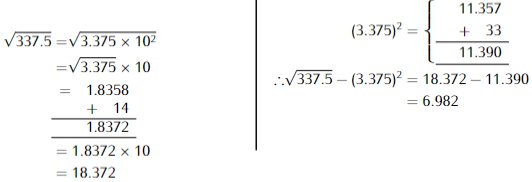
\includegraphics{images/Decimals_Ex3.png}

}

\caption{Example 3}

\end{figure}%

\end{tcolorbox}

\begin{tcolorbox}[enhanced jigsaw, left=2mm, colframe=quarto-callout-note-color-frame, toptitle=1mm, opacitybacktitle=0.6, rightrule=.15mm, colbacktitle=quarto-callout-note-color!10!white, colback=white, arc=.35mm, breakable, leftrule=.75mm, bottomtitle=1mm, bottomrule=.15mm, title=\textcolor{quarto-callout-note-color}{\faInfo}\hspace{0.5em}{Problem to Solve}, titlerule=0mm, coltitle=black, toprule=.15mm, opacityback=0]

\begin{enumerate}
\def\labelenumi{\arabic{enumi}.}
\item
  Use the tables of squares and square roots only to find the value of:
  (2mks) \[
  \left(0.0546\right)^{\frac{1}{2}}  
  \]
\item
  Evaluate without using a calculator. (3mks) \[
  \frac{23.4-2(5.2+5.3)}{3.2\times 1.2}
  \]
\item
  Use square tables to evaluate, to 4 significant figures. (2mks) \[
  \left(8.254\right)^2  
  \]
\item
  Evaluate without using tables or calculator. (3mks) \[
  \frac{2.5\times\sqrt[]{324}}{3\times\sqrt[]{729}} 
  \]
\item
  Find the exact value of:(3mks)
\end{enumerate}

\[
    2.\dot{4}\dot{1}-0.\dot{3}\dot{2}
\]

\begin{enumerate}
\def\labelenumi{\arabic{enumi}.}
\setcounter{enumi}{5}
\item
  The number \(5.\dot{8}\dot{1}\) contains an integral part and a
  recurring decimal. Convert the number into an improper fraction and
  hence a mixed fraction.\hspace{7cm} \((3mks)\)
\item
  Without using a calculator or mathematical tables find the value
  of:(3mks) \[
  \frac{0.0060\times2.4\times0.3^2}{0.9\times0.00015\times160} 
  \]
\item
  Express the recurring decimal below as a fraction;
  \(0.3\dot{7}\dot{2}\) leaving your answer in the form of
  \(\frac{a}{b}\) where \(a\) and \(b\) are integers.(3mks)
\item
  Use the square and square-root tables to evaluate to 4 significant
  figures the expression. (4mks) \[
  \left(43.46\right)^2-\sqrt[]{3785.4}
  \]
\item
  Using tables of square roots and reciprocals, evaluate: (3mks) \[
  \sqrt[]{0.1964}+(0.478)^2
  \]
\item
  Convert \(0.63\dot{3}\dot{1}\) into a fraction without using a
  calculator. \hspace{4.75cm} \((3mks)\)
\item
  Use square and square root tables to calculate to 3 significant
  figures the value of: (4mks) \[
  \sqrt[]{\left(0.04766\right)^2-(0.00972)^2}  
  \]
\item
  Use square roots and square tables to evaluate the expression: (3mks)
  \[
  \left(0.005467\right)^2+\left(0.04328\right)^2 \hspace{9.95cm} 
  \]
\item
  The surface area of a sphere of radius,r is given by the formula
  \(A = 4\pi r^2\). using square root tables, calculate the radius of
  the sphere whose surface area is \(120 cm^2\) \hspace{3.2cm}
  \((3mks)\)
\item
  The periodic time for the swing of a pendulum in seconds is given by
  the formula,\(T =2\pi\sqrt[]{\frac{l}{g}}\). Using square root tables,
  calculate the value of \(T\) when \(l = 23.7cm\) and
  \(g = 1000 cms^{-2}\). \hspace*{14.2cm} \((3mks)\)
\end{enumerate}

\end{tcolorbox}

\bookmarksetup{startatroot}

\chapter{Chapter Eight: Algebraic
Expressions}\label{chapter-eight-algebraic-expressions}

\bookmarksetup{startatroot}

\chapter*{Algebraic Expressions}\label{algebraic-expressions}
\addcontentsline{toc}{chapter}{Algebraic Expressions}

\markboth{Algebraic Expressions}{Algebraic Expressions}

\textbf{Algebraic expression}, is an expression built up from integer
constants, variables, and algebraic operations (Addition, subtraction,
division and multiplication).

\section{Solved problems}\label{solved-problems}

\begin{tcolorbox}[enhanced jigsaw, left=2mm, colframe=quarto-callout-note-color-frame, toptitle=1mm, opacitybacktitle=0.6, rightrule=.15mm, colbacktitle=quarto-callout-note-color!10!white, colback=white, arc=.35mm, breakable, leftrule=.75mm, bottomtitle=1mm, bottomrule=.15mm, title=\textcolor{quarto-callout-note-color}{\faInfo}\hspace{0.5em}{Example 1}, titlerule=0mm, coltitle=black, toprule=.15mm, opacityback=0]

Simplify the following:

\end{tcolorbox}

\begin{tcolorbox}[enhanced jigsaw, left=2mm, colframe=quarto-callout-note-color-frame, toptitle=1mm, opacitybacktitle=0.6, rightrule=.15mm, colbacktitle=quarto-callout-note-color!10!white, colback=white, arc=.35mm, breakable, leftrule=.75mm, bottomtitle=1mm, bottomrule=.15mm, title=\textcolor{quarto-callout-note-color}{\faInfo}\hspace{0.5em}{Example 1 (a)}, titlerule=0mm, coltitle=black, toprule=.15mm, opacityback=0]

a) \[\frac{2m-am-2y+ay}{2m+2y-am-ay}  (3 mks)\]

\end{tcolorbox}

\begin{tcolorbox}[enhanced jigsaw, left=2mm, colframe=quarto-callout-caution-color-frame, toptitle=1mm, opacitybacktitle=0.6, rightrule=.15mm, colbacktitle=quarto-callout-caution-color!10!white, colback=white, arc=.35mm, breakable, leftrule=.75mm, bottomtitle=1mm, bottomrule=.15mm, title=\textcolor{quarto-callout-caution-color}{\faFire}\hspace{0.5em}{Solution}, titlerule=0mm, coltitle=black, toprule=.15mm, opacityback=0]

Factorizing the \textbf{Numerator:}

\begin{equation}
\begin{split}
2m - am - 2y + ay & = m(2-a) - y(2-a) \\
& = (m-y)(2-a) \\
\end{split}
\end{equation}

Factorizing the \textbf{Denominator:}

\begin{equation}
\begin{split}
2m + 2y - am - ay &= 2(m+y) - a(m+y) \\
&= (2-a)(m+y) \\
\Rightarrow \, \frac{(m-y)\cancel{(2-a)}}{\cancel{(2-a)}(m+y)} &= \frac{(m-y)}{(m+y)}
\end{split}
\end{equation}

\end{tcolorbox}

\begin{tcolorbox}[enhanced jigsaw, left=2mm, colframe=quarto-callout-note-color-frame, toptitle=1mm, opacitybacktitle=0.6, rightrule=.15mm, colbacktitle=quarto-callout-note-color!10!white, colback=white, arc=.35mm, breakable, leftrule=.75mm, bottomtitle=1mm, bottomrule=.15mm, title=\textcolor{quarto-callout-note-color}{\faInfo}\hspace{0.5em}{Example 1 (b)}, titlerule=0mm, coltitle=black, toprule=.15mm, opacityback=0]

b) \[\frac{x^2-4ax-4a+x}{(x+1)(4a^2-ax)}  (3 mks)\]

\end{tcolorbox}

\begin{tcolorbox}[enhanced jigsaw, left=2mm, colframe=quarto-callout-caution-color-frame, toptitle=1mm, opacitybacktitle=0.6, rightrule=.15mm, colbacktitle=quarto-callout-caution-color!10!white, colback=white, arc=.35mm, breakable, leftrule=.75mm, bottomtitle=1mm, bottomrule=.15mm, title=\textcolor{quarto-callout-caution-color}{\faFire}\hspace{0.5em}{Solution}, titlerule=0mm, coltitle=black, toprule=.15mm, opacityback=0]

Factorizing the \textbf{Numerator:}

\begin{equation}
\begin{split}
x^2 - 4ax - 4a + x & = x(x - 4a) + 1(x - 4a) \\ 
& = (x + 1)(x - 4a) \\ 
\end{split}
\end{equation}

\textbf{Denominator:}

\begin{equation}
\begin{split}
(x+1)(4a^2 - ax) \\ 
\Rightarrow \frac{\cancel{(x+1)}(x - 4a)}{\cancel{(x+1)}(4a^2 - ax)} &= \frac{x - 4a}{a(4a - x)} \\ 
&= \frac{\cancel{x - 4a}}{-a(\cancel{x - 4a})} \\ 
&= \frac{-1}{a} 
\end{split}
\end{equation}

\end{tcolorbox}

\begin{tcolorbox}[enhanced jigsaw, left=2mm, colframe=quarto-callout-note-color-frame, toptitle=1mm, opacitybacktitle=0.6, rightrule=.15mm, colbacktitle=quarto-callout-note-color!10!white, colback=white, arc=.35mm, breakable, leftrule=.75mm, bottomtitle=1mm, bottomrule=.15mm, title=\textcolor{quarto-callout-note-color}{\faInfo}\hspace{0.5em}{Example 1 (c)}, titlerule=0mm, coltitle=black, toprule=.15mm, opacityback=0]

c) \[\frac{x-2y}{12p}-\frac{x+3y}{60p}   (3 mks)\]

\end{tcolorbox}

\begin{tcolorbox}[enhanced jigsaw, left=2mm, colframe=quarto-callout-caution-color-frame, toptitle=1mm, opacitybacktitle=0.6, rightrule=.15mm, colbacktitle=quarto-callout-caution-color!10!white, colback=white, arc=.35mm, breakable, leftrule=.75mm, bottomtitle=1mm, bottomrule=.15mm, title=\textcolor{quarto-callout-caution-color}{\faFire}\hspace{0.5em}{Solution}, titlerule=0mm, coltitle=black, toprule=.15mm, opacityback=0]

\begin{equation}
\begin{split}
\text{L.C.M} & = 60p \\ 
\frac{x - 2y}{12p} - \frac{x + 3y}{60p} & = \frac{5(x - 2y) - (x + 3y)}{60p} \\ 
& = \frac{5x - 10y - x - 3y}{60p} \\ 
& = \frac{4x - 13y}{60p} 
\end{split}
\end{equation}

\end{tcolorbox}

\begin{tcolorbox}[enhanced jigsaw, left=2mm, colframe=quarto-callout-note-color-frame, toptitle=1mm, opacitybacktitle=0.6, rightrule=.15mm, colbacktitle=quarto-callout-note-color!10!white, colback=white, arc=.35mm, breakable, leftrule=.75mm, bottomtitle=1mm, bottomrule=.15mm, title=\textcolor{quarto-callout-note-color}{\faInfo}\hspace{0.5em}{Example 2}, titlerule=0mm, coltitle=black, toprule=.15mm, opacityback=0]

Given that p=4, q=-3, and r=-1 find the value of:
\[\frac{2pqr^4+pqr-pr}{4pr-2qr+2pqr}  (3mks) \]

\end{tcolorbox}

\begin{tcolorbox}[enhanced jigsaw, left=2mm, colframe=quarto-callout-caution-color-frame, toptitle=1mm, opacitybacktitle=0.6, rightrule=.15mm, colbacktitle=quarto-callout-caution-color!10!white, colback=white, arc=.35mm, breakable, leftrule=.75mm, bottomtitle=1mm, bottomrule=.15mm, title=\textcolor{quarto-callout-caution-color}{\faFire}\hspace{0.5em}{Solution}, titlerule=0mm, coltitle=black, toprule=.15mm, opacityback=0]

\textbf{Numerator:}

\begin{equation}
\begin{split}
2pqr^4 + pqr - pr & = 2(4)(-3)(-1)^4 + (4)(-3)(-1) - (4)(-1) \\ 
& = 2(4)(-3)(1) + (4)(-3)(-1) - (4)(-1) \\ 
& = -24 + 12 + 4 \\ 
& = -8 \\ 
\end{split}
\end{equation}

\textbf{Denominator:}

\begin{equation}
\begin{split}
4pr - 2qr + 2pqr & = 4(4)(-1) - 2(-3)(-1) + 2(4)(-3)(-1) \\ 
& = -16 - 6 + 24 \\ 
& = 2 \\ 
\therefore \frac{\cancelto{-4}{-8}}{\cancel{2}} & = -4 
\end{split}
\end{equation}

\end{tcolorbox}

\begin{tcolorbox}[enhanced jigsaw, left=2mm, colframe=quarto-callout-note-color-frame, toptitle=1mm, opacitybacktitle=0.6, rightrule=.15mm, colbacktitle=quarto-callout-note-color!10!white, colback=white, arc=.35mm, breakable, leftrule=.75mm, bottomtitle=1mm, bottomrule=.15mm, title=\textcolor{quarto-callout-note-color}{\faInfo}\hspace{0.5em}{Example 3}, titlerule=0mm, coltitle=black, toprule=.15mm, opacityback=0]

Simplify

\[\frac{(4a+b)^2-(b-4a)^2}{(a+b)^2-(b-a)^2}   (4mks) \]

\end{tcolorbox}

\begin{tcolorbox}[enhanced jigsaw, left=2mm, colframe=quarto-callout-caution-color-frame, toptitle=1mm, opacitybacktitle=0.6, rightrule=.15mm, colbacktitle=quarto-callout-caution-color!10!white, colback=white, arc=.35mm, breakable, leftrule=.75mm, bottomtitle=1mm, bottomrule=.15mm, title=\textcolor{quarto-callout-caution-color}{\faFire}\hspace{0.5em}{Solution}, titlerule=0mm, coltitle=black, toprule=.15mm, opacityback=0]

\textbf{Numerator}:

\begin{equation}
\begin{split}
(4a + b)^2 & = (4a + b)(4a + b) \\ 
& = 4a(4a + b) + b(4a + b) \\ 
& = 16a^2 + 4ab + 4ab + b^2 \\ 
& = 16a^2 + 8ab + b^2 \\ 
(b - 4a)^2 & = (b - 4a)(b - 4a) \\ 
& = b(b - 4a) - 4a(b - 4a) \\ 
& = b^2 - 4ab - 4ab + 16a^2 \\ 
& = b^2 - 8ab + 16a^2 \\ 
(4a + b)^2 - (b - 4a)^2 & = 16a^2 + 8ab + b^2 - (b^2 - 8ab + 16a^2) \\ 
& = 16a^2 + 8ab + b^2 - b^2 + 8ab - 16a^2 \\ 
& = 8ab + 8ab \\ 
& = 16ab \\ 
\end{split}
\end{equation}

\textbf{Denominator:}

\begin{equation}
\begin{split}
(a + b)^2 & = (a + b)(a + b) \\ 
& = a(a + b) + b(a + b) \\ 
& = a^2 + ab + ab + b^2 \\ 
& = a^2 + 2ab + b^2 \\ 
\\
(b - a)^2 & = (b - a)(b - a) \\ 
& = b(b - a) - a(b - a) \\ 
& = b^2 - ab - ab + a^2 \\ 
& = b^2 - 2ab + a^2 \\ 
\\
(a + b)^2 - (b - a)^2 & = a^2 + 2ab + b^2 - (b^2 - 2ab + a^2) \\ 
& = a^2 + 2ab + b^2 - b^2 + 2ab - a^2 \\ 
& = 2ab + 2ab \\ 
& = 4ab \\ 
\\
\therefore \frac{\cancelto{4}{16ab}}{\cancel{4ab}} & = 4 \\ 
\end{split}
\end{equation}

\end{tcolorbox}

\begin{tcolorbox}[enhanced jigsaw, left=2mm, colframe=quarto-callout-note-color-frame, toptitle=1mm, opacitybacktitle=0.6, rightrule=.15mm, colbacktitle=quarto-callout-note-color!10!white, colback=white, arc=.35mm, breakable, leftrule=.75mm, bottomtitle=1mm, bottomrule=.15mm, title=\textcolor{quarto-callout-note-color}{\faInfo}\hspace{0.5em}{Example 4}, titlerule=0mm, coltitle=black, toprule=.15mm, opacityback=0]

Solve the equation\\
\[\frac{3}{2r}=\frac{5}{5r-1}         (2mks)\]

\end{tcolorbox}

\begin{tcolorbox}[enhanced jigsaw, left=2mm, colframe=quarto-callout-caution-color-frame, toptitle=1mm, opacitybacktitle=0.6, rightrule=.15mm, colbacktitle=quarto-callout-caution-color!10!white, colback=white, arc=.35mm, breakable, leftrule=.75mm, bottomtitle=1mm, bottomrule=.15mm, title=\textcolor{quarto-callout-caution-color}{\faFire}\hspace{0.5em}{Solution}, titlerule=0mm, coltitle=black, toprule=.15mm, opacityback=0]

Multiply both sides by the L.C.M of the \textbf{denominator}

\begin{equation}
\begin{split}
L.C.M &=2r(5r-1)\\
\frac{3(\cancel{2r}(5r-1))}{\cancel{2r}}&=\frac{5(2r(\cancel{5r-1}))}{\cancel{5r-1}}\\
3(5r-1)&=5(2r)\\ 
15r-3&=10r\\
15r-10r&=3\\
\frac{\cancel5r}{\cancel5}&=\frac{3}{5}\\ \therefore r&=\frac{3}{5}\\
\end{split}
\end{equation}

\end{tcolorbox}

\begin{tcolorbox}[enhanced jigsaw, left=2mm, colframe=quarto-callout-note-color-frame, toptitle=1mm, opacitybacktitle=0.6, rightrule=.15mm, colbacktitle=quarto-callout-note-color!10!white, colback=white, arc=.35mm, breakable, leftrule=.75mm, bottomtitle=1mm, bottomrule=.15mm, title=\textcolor{quarto-callout-note-color}{\faInfo}\hspace{0.5em}{Example 5}, titlerule=0mm, coltitle=black, toprule=.15mm, opacityback=0]

In fourteen years' time, a mother will be twice as old as her son. Four
years ago, the sum of their ages was 30 years. Find how old the mother
was when the son was born.\((4 mks)\)

\end{tcolorbox}

\begin{tcolorbox}[enhanced jigsaw, left=2mm, colframe=quarto-callout-caution-color-frame, toptitle=1mm, opacitybacktitle=0.6, rightrule=.15mm, colbacktitle=quarto-callout-caution-color!10!white, colback=white, arc=.35mm, breakable, leftrule=.75mm, bottomtitle=1mm, bottomrule=.15mm, title=\textcolor{quarto-callout-caution-color}{\faFire}\hspace{0.5em}{Solution}, titlerule=0mm, coltitle=black, toprule=.15mm, opacityback=0]

\begin{equation}
\begin{split}
\underline{14 \,yrs \,time:} \\
Mother&=2x\\ son&=x\\
\underline{ Present\, age:}\\
Mother&=2x-14\\ Son&=x-14\\
\underline{4 \, yrs\, ago:}\\ 
Mother&=2x-14-4\\Son&=x-14-4\\ 
\end{split}
\end{equation}

\begin{equation}
\begin{split}
\underline{Sum \,of\, their\, age:}\\
(2x-18)+(x-18)&=30\\3x-36&=30\\
\frac{\cancel{3}x}{\cancel{3}}&=\cancelto{\frac{22}{1}}{\frac{66}{3}}\\&=22, years\\ 
Mother \Rightarrow (44-14)&= 30 \,years\, now\\
Son \Rightarrow (22-14)&= 8 \,years\, now\\ Mother's\, age\, when\, giving \,birth&=30-8\\&=22\,years
\end{split}
\end{equation}

\(\therefore\) The mother was 22 years old when the son was born.

\end{tcolorbox}

\begin{tcolorbox}[enhanced jigsaw, left=2mm, colframe=quarto-callout-note-color-frame, toptitle=1mm, opacitybacktitle=0.6, rightrule=.15mm, colbacktitle=quarto-callout-note-color!10!white, colback=white, arc=.35mm, breakable, leftrule=.75mm, bottomtitle=1mm, bottomrule=.15mm, title=\textcolor{quarto-callout-note-color}{\faInfo}\hspace{0.5em}{Problems to Solve}, titlerule=0mm, coltitle=black, toprule=.15mm, opacityback=0]

\begin{enumerate}
\def\labelenumi{\arabic{enumi}.}
\item
  Esther has \(26\) coins whose total value is \(Ksh.\,205\). There are
  thrice as many \(Ksh.\,10\) coins as there are \(Ksh.\,20\) coins. The
  rest are 50cts coins. Find the number of \(Ksh.\,20\) coins that
  Esther has. \((3mks)\)
\item
  Joyce has 21 coins whose total value is \(Ksh. \,72\). There are twice
  as many five shillings coins as there are ten shillings coins. The
  rest are one shilling coin. Find the number of ten shillings coins
  that Joyce has. \((3 mks)\)
\item
  A rectangular plot is \(0.4 m\) longer than it is wide. If its length
  is \(6m\) find its perimeter. When the breadth of the rectangle is
  reduced by \(0.5m\), the length is increased such that the perimeter
  is increased by \(\frac{1}{4}\) of its original. What is the change in
  the length of the rectangle? \((3 mks)\)
\item
  Three fruit vendors Musa, Florence, and Josephine agreed to share
  \(Ksh.\,1800\) gained after a sale of the property. For every
  \(Ksh.\, 1\) that Musa gets, Florence gets 50cts and for every
  \(Ksh.\,2\) that Florence gets Josephine gets \(Ksh.\,3\). Find
  Florence's share. \((3mks)\)
\item
  Three-fifths of the work is done on the first day. On the second day,
  \(\frac{3}{4} \,\)of the remainder is completed. If on the third day
  \(\frac{7}{8} \,\)of what remained is done, what fraction of the work
  still remains to be done? \((3mks)\)
\item
  Three years ago, Albina was three times as old as her son. In five
  years' time, the sum of their ages will be 76. Determine their present
  ages. \((3mks)\)
\item
  Simplify \((3mks)\)
\end{enumerate}

\[\frac{(4p+2q)^2-(2q-4p)^2}{(2p+q)^2-(q-2p)^2} \]

\begin{enumerate}
\def\labelenumi{\arabic{enumi}.}
\setcounter{enumi}{7}
\item
  In a poultry farm, there are eight more hens than ducks, three times
  as many turkeys as hens, and three-quarters as many quails as turkeys.

  a) If there are x ducks, write down a simplified expression in x for
  the total number of birds on the farm. \((1mk)\)

  b) Find the total number of birds given that there are 162 quails.
  \((2mks)\)
\item
  Jane's mother is now four times as older than her. In eight years'
  time, she will be three times as old as her daughter. Find their
  present ages. \((3mks)\)
\item
  Factorize completely \(3mks)\)
\end{enumerate}

\[
(p-2q)(3p+2q)-(p-2q)^2
\] 11. Simplify the following expression by reducing it to a single
fraction \((3 mks)\)

\[
\frac{4p-3}{3}-\frac{3p-4}{4}=\frac{3-p}{6}
\]

\begin{enumerate}
\def\labelenumi{\arabic{enumi}.}
\setcounter{enumi}{11}
\item
  After work a hawker had four times as many ten-shilling coins as
  twenty-shilling coins, eight times as many five-shilling coins as
  twenty-shilling coins and thrice as many one-shilling coins as
  ten-shilling coins. After counting his money he found that he had a
  total of \(Ksh.\, 560\). Calculate the number of coins he had.
  \((3mks)\)
\item
  Osinya is now two times as old as his younger brother and three times
  as old as his son. Four years from now Osinya's age will be twelve
  years more than the sum of the ages of his son and younger brother.
  Find Osinya and his son present age.\((4mks)\)
\item
  Wathitha is now three times as old as Fatuma. Seven years ago Wathitha
  was exactly two-third times as old as Fatuma will be 14 years from
  now. Find Wathitha's present age. \(3mks)\)
\item
  Fadhili is now two and a half times as old as his son. Sixteen years
  ago his age was 7 years more than his son will be 7 years from now.
  Calculate Fadhili's present age. \(3mks)\)
\item
  In a church harambee meeting, there were 300 people present. Each man
  contributed \(Ksh. \,500\) and each woman \(Ksh.\, 300\). The meeting
  raised a total of \(Ksh.\, 100,200\). Calculate the number of men
  present in the meeting. \(3mks)\)
\item
  A group of 144 women and young girls in a certain church organized a
  trip to Kisumu. Each woman paid \(Ksh. \,900\) while each girl paid
  half as much. In this way the group raised a total of
  \(Ksh.\, 81,000\) for the trip. Calculate the number of women in the
  group. \((3mks)\)
\item
  The sum of age's three children of Awiti, Wafula, and Najala is 68
  years. Wafula is three-quarter as old as Awiti and twice times as old
  as Najala. Determine their ages. \((3mks)\)
\item
  Mwangi working on a coffee factory is paid \(Ksh.\, 40\) for every
  normal working hour and \(Ksh.\, 60\) for each hour worked overtime.
  During one week he worked for a total of 80 hours and was paid
  \(Ksh. \,3840\) in wages. Determine the number of hours he worked
  overtime. \((3mks)\)
\item
  A retailer has bought a mixture of bags of beans and bags of peas from
  a wholesaler. One bag of beans has a mass of 90 Kg and one bag of peas
  has a mass of 75 Kg. the retailer bought 350 bags whose total mass is
  28.5 tonnes. Find the number of bags of each type he bought.
  \((3mks)\)
\item
  Given that \(x=4,\, y= -3 ,\, and \,\,z= -1\) evaluate. \((6mks)\)

  a) \[ \frac{2(x+z)^2-(x-y)(y-z)}{3(x+y)-2(y-z)}\]

  b) \[
  \frac{2xy^2-3xy^2z^2-3xy^2z}{x^2yz-2xyz^2-4xyz}
  \]
\item
  In a certain year, Waithera had 5 times as many goats as cows and
  three-quarter as many sheep as goats. In the next year the number of
  goats increased by 24\%, the number of cows decreased by 50\% while
  the number of sheep decreased by 30\%. At the end of the preceding
  year Waithera had a total of 1865 animals. Calculate to three
  significant figures the percentage decrease in the total number of
  animals during the preceding year. \((10mks)\)
\item
  A family has two children whose age difference is 9. Twice the sum of
  their ages is equal to the age of their father.

  a) By letting the age of the younger child be x, write an expression
  of the:

  i) Age of the elder child. \((1mk)\)

  ii) Age of their father. \((1mk)\)

  iii) If in 19 years' time, the product of the ages of the two children
  is equal to 14 times the age of their father; form an equation in x
  and hence determine the present possible age of the younger child.
  \((4mks)\)

  iv) Determine the possible age of the elder child in 19 years' time.
  \((2mks)\)

  v) Find the possible age of the father. \((2mks)\)
\item
  A group of women decided to raise \(Ksh. \, 480, 000\) to buy a piece
  of plot costing \(Ksh.\, 80, 000\) per hectare. Before the actual
  payment was made, four of the women pulled out and each of those
  remaining had to pay an additional \(Ksh. \,20, 000\).

  a) If the original number of the women in the group was \(x\), write
  down;

  i) An expression of how much each was to contribute originally.
  \((1mks)\)

  ii) An expression of how the remaining number of women were to
  contribute after the four pulled out. \((1mks)\)

  b) Determine the number of women who actually contributed towards the
  purchase of the plot. \((5mks)\)

  c) Calculate the ration of the supposed original contribution to the
  new contribution. \((1mks)\)

  d) If the plot was sub-divided equally, find the size of the plot each
  woman got.\((2mks)\)
\end{enumerate}

\end{tcolorbox}

\bookmarksetup{startatroot}

\chapter{Chapter Nine: Rate, Ratio, Proportion, and
Percentage}\label{chapter-nine-rate-ratio-proportion-and-percentage}

\bookmarksetup{startatroot}

\chapter*{Rate, Ratio, Proportion, and
Percentage}\label{rate-ratio-proportion-and-percentage}
\addcontentsline{toc}{chapter}{Rate, Ratio, Proportion, and Percentage}

\markboth{Rate, Ratio, Proportion, and Percentage}{Rate, Ratio,
Proportion, and Percentage}

\textbf{Rate}, is a comparison of one quantity with another of a
different kind. If a van takes three hours to travel a distance of
\(180 \,Km\), then the van is traveling at an average rate of
\(60 \,Km/hr\).

\textbf{Ratio}, is a way of comparing two similar quantities. If John is
7 years old and his sister Jane is 16 years old, then John's age is
\(\frac{7}{16}\) of Jane's age and the ratio of their ages is 7:16. In
stating the ratio the unit must be the same.

\textbf{Proportion}, is a comparison of two or more ratios. For example,
if a, b, and c are three numbers such that \$ a:b:c = 3:5:7\$ then a, b,
and c are said to be proportional to 3, 5, and 7 and the relationship
should be integrated to mean \(\frac{a}{3}=\frac{b}{5}=\frac{c}{7}\). In
the same way,\$ a:b =3:5, b:c = 5:7,\$ and \(a:c = 3:7\).

\section{Solved Examples}\label{solved-examples-7}

\begin{tcolorbox}[enhanced jigsaw, left=2mm, colframe=quarto-callout-note-color-frame, toptitle=1mm, opacitybacktitle=0.6, rightrule=.15mm, colbacktitle=quarto-callout-note-color!10!white, colback=white, arc=.35mm, breakable, leftrule=.75mm, bottomtitle=1mm, bottomrule=.15mm, title=\textcolor{quarto-callout-note-color}{\faInfo}\hspace{0.5em}{Example 1}, titlerule=0mm, coltitle=black, toprule=.15mm, opacityback=0]

If ,\(a:b=3:5\) and \(b:c=7:9\), Find the ratio: \(a:c\).
\hspace{6.5 cm} \((3mks)\)

\end{tcolorbox}

\begin{tcolorbox}[enhanced jigsaw, left=2mm, colframe=quarto-callout-caution-color-frame, toptitle=1mm, opacitybacktitle=0.6, rightrule=.15mm, colbacktitle=quarto-callout-caution-color!10!white, colback=white, arc=.35mm, breakable, leftrule=.75mm, bottomtitle=1mm, bottomrule=.15mm, title=\textcolor{quarto-callout-caution-color}{\faFire}\hspace{0.5em}{Solution}, titlerule=0mm, coltitle=black, toprule=.15mm, opacityback=0]

\(a:b=3:5\)

\(b:c=7:9\)

\[
\begin{matrix}
  a&:&b&:&c \\
  7(3&:&5)\\
  \,&\,&\,(7&:&9)5\\ \\
  a&:&b&:&c \\
  21&:&35&:&45\\
 \end{matrix}
\] \(\therefore \, a:c=21:45\)

\end{tcolorbox}

\begin{tcolorbox}[enhanced jigsaw, left=2mm, colframe=quarto-callout-note-color-frame, toptitle=1mm, opacitybacktitle=0.6, rightrule=.15mm, colbacktitle=quarto-callout-note-color!10!white, colback=white, arc=.35mm, breakable, leftrule=.75mm, bottomtitle=1mm, bottomrule=.15mm, title=\textcolor{quarto-callout-note-color}{\faInfo}\hspace{0.5em}{Example 2}, titlerule=0mm, coltitle=black, toprule=.15mm, opacityback=0]

Twelve laborers each working six hours a day, take twelve days to plough
a piece of land. How long would it take 24 laborers each working 9 hours
a day to plough the same piece of land? \hspace{0.6cm} \((3mks)\)

\end{tcolorbox}

\begin{tcolorbox}[enhanced jigsaw, left=2mm, colframe=quarto-callout-caution-color-frame, toptitle=1mm, opacitybacktitle=0.6, rightrule=.15mm, colbacktitle=quarto-callout-caution-color!10!white, colback=white, arc=.35mm, breakable, leftrule=.75mm, bottomtitle=1mm, bottomrule=.15mm, title=\textcolor{quarto-callout-caution-color}{\faFire}\hspace{0.5em}{Solution}, titlerule=0mm, coltitle=black, toprule=.15mm, opacityback=0]

\[
\begin{matrix}
  men&\,&hours&\,&days\\
  12&\,&6&\,&12\\
  24&\,&9&\,&?
 \end{matrix}
\] 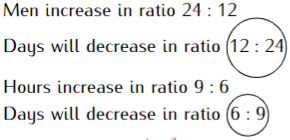
\includegraphics{images/Ratio_Ex2.png}

\[Days\, needed: \cancelto{\frac{1}{2}}{\frac{12}{24}}\times\cancelto{\frac{2}{3}}{\frac{6}{9}}\times12=4\]
\(\therefore\) The laborers would take \(4\) days

\end{tcolorbox}

\begin{tcolorbox}[enhanced jigsaw, left=2mm, colframe=quarto-callout-note-color-frame, toptitle=1mm, opacitybacktitle=0.6, rightrule=.15mm, colbacktitle=quarto-callout-note-color!10!white, colback=white, arc=.35mm, breakable, leftrule=.75mm, bottomtitle=1mm, bottomrule=.15mm, title=\textcolor{quarto-callout-note-color}{\faInfo}\hspace{0.5em}{Example 3}, titlerule=0mm, coltitle=black, toprule=.15mm, opacityback=0]

A blend of juice is made from mango and passion. The cost of four limes
of mango is \(Ksh.\, 180\) and two limes of passion is \(Ksh. \,160\).
In what ratio should the juice be mixed such that by selling the mixture
at \(Ksh.\, 90\) per lime, a profit of 20\% is realized? \hspace{5.5 cm}
\((3 mks)\)

\end{tcolorbox}

\begin{tcolorbox}[enhanced jigsaw, left=2mm, colframe=quarto-callout-caution-color-frame, toptitle=1mm, opacitybacktitle=0.6, rightrule=.15mm, colbacktitle=quarto-callout-caution-color!10!white, colback=white, arc=.35mm, breakable, leftrule=.75mm, bottomtitle=1mm, bottomrule=.15mm, title=\textcolor{quarto-callout-caution-color}{\faFire}\hspace{0.5em}{Solution}, titlerule=0mm, coltitle=black, toprule=.15mm, opacityback=0]

\begin{tabular}{|l|c|c|r|}
\hline
Juice&Mango&Passion&Blend\\
\hline
Ratio&1&n&$1+n$\\
\hline
cost  per litre&45&80&\,\\
\hline
Total cost&45&80n&45+80n\\
\hline
\end{tabular}

\[
\begin{split}
Buying \,price (B.P) \Rightarrow \frac{45+80n}{1+n}&=100\%\\
Selling \,Price (S.P) \Rightarrow 90&=120\%\\
B.P \Rightarrow \frac{90\times 10\cancel{0}}{12\cancel{0}}&=75\\
\frac{45+80n}{1+n}&=75\\
\end{split}
\]

\[
\begin{split}
45+80n&=75+75n \\5n&=30\\
\frac{\cancel{5}n}{\cancel5}&=\frac{\cancelto{6}{30}}{\cancel5}\\
\frac{n}{1}&=\frac{6}{1}\\
\Rightarrow \frac{1}{n}&=\frac{1}{6}\\
\therefore 1:n&=1:6
\end{split}
\]

\end{tcolorbox}

\begin{tcolorbox}[enhanced jigsaw, left=2mm, colframe=quarto-callout-note-color-frame, toptitle=1mm, opacitybacktitle=0.6, rightrule=.15mm, colbacktitle=quarto-callout-note-color!10!white, colback=white, arc=.35mm, breakable, leftrule=.75mm, bottomtitle=1mm, bottomrule=.15mm, title=\textcolor{quarto-callout-note-color}{\faInfo}\hspace{0.5em}{Example 4}, titlerule=0mm, coltitle=black, toprule=.15mm, opacityback=0]

A cold water tap can fill a bath in 15 minutes while a hot water tap can
fill it in 10 minutes. The drainage pipe can empty it in 8 minutes. The
cold water and hot water taps are opened for 2 minutes. After two
minutes all three taps are opened. Find the total time taken to fill the
bath. \hspace {14.8 cm} \((3 mks)\)

\end{tcolorbox}

\begin{tcolorbox}[enhanced jigsaw, left=2mm, colframe=quarto-callout-caution-color-frame, toptitle=1mm, opacitybacktitle=0.6, rightrule=.15mm, colbacktitle=quarto-callout-caution-color!10!white, colback=white, arc=.35mm, breakable, leftrule=.75mm, bottomtitle=1mm, bottomrule=.15mm, title=\textcolor{quarto-callout-caution-color}{\faFire}\hspace{0.5em}{Solution}, titlerule=0mm, coltitle=black, toprule=.15mm, opacityback=0]

\textbf{The 3 taps rate of filling the bath in 1 min:}

\begin{equation}
\begin{split}
\text{Cold water tap} & = \frac{1}{15} \\ 
\text{Hot water tap} & = \frac{1}{10} \\ 
\text{Drainage tap} & = \frac{1}{8} \\ 
\\
\textbf{Fraction by hot and cold tap in 2 min:} \\ 
\left( \frac{1}{15} + \frac{1}{10} \right) \cdot 2 & = \frac{1}{3} 
\end{split}
\end{equation}

\textbf{Fraction of water unfilled}:

\[\Rightarrow 1-\frac{1}{3}=\frac{2}{3}\]

\textbf{Fraction of water by 3 taps in 1 min:}

\[\frac{1}{15}+\frac{1}{10}-\frac{1}{8}=\frac{1}{24}\]

\textbf{Time to fill the remaining water:}

\[\frac{2}{3}\div \frac{1}{24}\Rightarrow \frac{2}{\cancel{3}} \times \cancel{24}^8=16 \]

\(\therefore\) Total time \(\Rightarrow 16+2=18\) min.

\end{tcolorbox}

\begin{tcolorbox}[enhanced jigsaw, left=2mm, colframe=quarto-callout-note-color-frame, toptitle=1mm, opacitybacktitle=0.6, rightrule=.15mm, colbacktitle=quarto-callout-note-color!10!white, colback=white, arc=.35mm, breakable, leftrule=.75mm, bottomtitle=1mm, bottomrule=.15mm, title=\textcolor{quarto-callout-note-color}{\faInfo}\hspace{0.5em}{Example 5}, titlerule=0mm, coltitle=black, toprule=.15mm, opacityback=0]

A plastic container manufacturer increased the radius of a cylindrical
can by 22.5\% but, decreased its height by 30\%. Calculate in two
decimal places the percentage increase in the volume of the can.
\hspace{15cm}\((3mks)\)

\end{tcolorbox}

\begin{tcolorbox}[enhanced jigsaw, left=2mm, colframe=quarto-callout-caution-color-frame, toptitle=1mm, opacitybacktitle=0.6, rightrule=.15mm, colbacktitle=quarto-callout-caution-color!10!white, colback=white, arc=.35mm, breakable, leftrule=.75mm, bottomtitle=1mm, bottomrule=.15mm, title=\textcolor{quarto-callout-caution-color}{\faFire}\hspace{0.5em}{Solution}, titlerule=0mm, coltitle=black, toprule=.15mm, opacityback=0]

\begin{equation}
\begin{split}
\text{Volume} & = \pi r^2 h \\ 
\text{Old volume} & = \pi r^2 h \\ 
\\
\text{New radius} & = 1.225r \\ 
\text{New height} & = 0.7h \\ 
\\
\text{New volume} & = \pi(1.225r)^2(0.7h) \\ 
& = 1.225^2 \times 0.7 \times r^2 \times h \\ 
& \approx 1.05044 \pi r^2 h 
\end{split}
\end{equation}

\begin{equation}
\begin{split}
Volume\, increase&=1.05044\pi r^2h-\pi r^2h\\
&=0.05044\pi r^2h\\
Percentage \,increase &=\frac{Increase}{Old \,volume}\times 100\\
&=\frac{0.05044\cancel{\pi r^2h}}{\cancel{\pi r^2h}}\times 100\\ 
&\approx5.044\% \\ 
\therefore \% \,increase&=5.04\%
\end{split}
\end{equation}

\end{tcolorbox}

\begin{tcolorbox}[enhanced jigsaw, left=2mm, colframe=quarto-callout-note-color-frame, toptitle=1mm, opacitybacktitle=0.6, rightrule=.15mm, colbacktitle=quarto-callout-note-color!10!white, colback=white, arc=.35mm, breakable, leftrule=.75mm, bottomtitle=1mm, bottomrule=.15mm, title=\textcolor{quarto-callout-note-color}{\faInfo}\hspace{0.5em}{Problems to Solve}, titlerule=0mm, coltitle=black, toprule=.15mm, opacityback=0]

\begin{enumerate}
\def\labelenumi{\arabic{enumi}.}
\item
  A photograph is reduced in the ratio \(2:7\) for a newspaper, and
  further reduced in the ratio \(5:7\) for an exercise book. Find the
  ratio of the newspaper size to textbook size. \hspace{2 cm} \((3mks)\)
\item
  Five plows working 8 hours daily complete a piece of work in 6 days.
  How long will it take 12 plows working 5 hours a day to complete the
  same work? \hspace{4.6 cm} \((2mks)\)
\item
  There are two grades of beans, grade A and grade B. Grade A costs
  \(Ksh. \,100\) per kg and grade B costs \(Ksh.\, 80\) per kg. In what
  ratio must the two grades be mixed in order to produce a blend worth
  \(Ksh.\, 95\) per kg? \hspace{10.6cm} \((3mks)\)
\item
  A tradesman blends 340kg of tea costing \(Ksh. \,80\) per kg with
  160kg of tea costing \(Ksh.\, 100\) per kg. At what price must he sell
  the mixture, to make a 25\% profit? \hspace{3.6cm} \((3mks)\)
\item
  Oil flows through a pipe whose cross-sectional radius is 7cm at a rate
  of 2m/min. Calculate how long it will take the pipe to fill a 28,000
  litres tank. \hspace{5.5cm} \((3 mks)\)
\item
  Nyamu and Gatungo working together can do a piece of work in 6 days.
  Gatungo working alone would take 10 days to complete the work. They
  start working together but, after 4 days Gatungo leaves and the
  remaining work is done by Nyamu. Find how long Nyamu takes to complete
  the remaining work. \hspace{11.5 cm} \((4mks)\)
\item
  Five constructors can build a 25-meter-long wall in 10 days. What
  length of wall can 10 constructors working at the same rate build in 8
  days? \hspace{5.8 cm} \((3mks)\)
\item
  A businesswoman bought 160 mangoes at \(Ksh. 50\) for every four
  mangoes. She sold some of them at \(Ksh. \,30\) for every three and
  the rest at \(Ksh.\, 30\) for every four. If she made a
  33\(\frac{1}{2}\)\% loss, calculate the number of mangoes sold at
  \(Ksh.\, 30\) for every four. \hspace{5 cm} \((3mks)\)
\item
  One hundred and twenty examiners each marking 90 papers per day are
  needed to mark an examination in 2 weeks. How many days would 180
  examiners each marking 35 papers per day take to mark the same
  examination? \hspace{8.2 cm} \((3mks)\)
\item
  A group of 15 soldiers set off with enough food to last 6 days. After
  6 soldiers evacuated. How many more days will the food last for the
  remaining soldiers? \hspace{4 cm} \((3 mks)\)
\item
  In the Moi University Christian Union choir, the ratio of male to
  female is \(2:3\). On one Sunday service, 10 male members were absent
  and six new female members joined the choir as guests for that day. If
  on this day the ratio of males to females was,\$ 1:3\$,, how many
  regular members does the choir have? \hspace{11.8 cm} \((3mks)\)
\item
  The ratio of men to women in Njega Boys High School B.O.G which
  consists of 45 members is \(7: 2\). Find the number of women required
  to join the existing members so that the ratio of men to women changes
  to \(5: 4\). \hspace{10.1cm} \((3mks)\)
\item
  A coffee trader mixes two brands of coffee, A and B to obtain 40kg of
  the mixture worth \(Ksh.\, 2,600\). If brand A is valued at
  \(Ksh.\, 70\) per kg and brand B is valued at \(Ksh.\, 55\) per kg.
  Calculate the ratio in its simplest form in which brands A and B are
  mixed. \hspace{3.7 cm} \((4mks)\)
\item
  Nyamu bought sorghum and millet at \(Ksh.\,65\) per kg and
  \(Ksh.\,40\) per kg respectively. He then mixed them and sold the
  mixture at \(Ksh.\,60\) per kg making a profit of 20\%. Determine the
  ratio of sorghum to millet in the mixture. \hspace{8.5 cm} \((3mks)\)
\item
  The ratio of a spherical balloon increases by 4\% as it rises up in
  the air. Find the percentage increase in its;

  a) Surface area. \hspace{11 cm} \((2mks)\)

  b) Volume \hspace{12 cm} \((2mks)\)
\item
  A dealer has two types of grades of tea, x and y. Grade x costs
  \(Ksh.\, 150\) per kg and grade y costs \(Ksh.\, 170\) per kg. If he
  mixes \(x\) and \(y\) in the ratio \(2:3\) to make a brand of tea
  which he sells at \(Ksh.\, 180\) per kg, calculate the percentage
  profit that he makes.\hspace{2.5cm} \((3 mks)\)
\item
  In what ratio will coffee grade A cost \(Ksh.\, 85\) per kg to be
  mixed with grade B costing \(Ksh.\,55\) per kg so that a profit of
  25\% is realized by selling the mixture at \(ksh.\,80\) per kg?
  \hspace{14.2cm} \((3mks)\)
\item
  A mixture contains two powders A and B with masses in the ration
  \(4: 10\). If the mixture costs \(Ksh.\, 650\) per kg and powder A
  costs \(Ksh. \,550\) per kg, find the cost of a kg of powder B.
  \hspace{14.1 cm} \((3 mks)\)
\item
  It would take 20 workers 12 days to spray a piece of land. If they
  work for 8 hours a day, how long will it take 24 workers if they work
  12 hours a day to three-quarters of the same land? \hspace{14.3cm}
  \((3mks)\)
\item
  A farmer has enough feed to last 35 pigs for 24 days. If he buys 5
  more pigs, how long will the feed last? \hspace{12.5 cm} \((3mks)\)
\item
  Mukami, a juice blender mixes two brands of Juice A and B to obtain
  90ml of the mixture worth \(Ksh.\, 165\) per litre. If brand A is
  valued at \(Ksh.\, 175\) per 1 litre bottle and brand B at
  \(Ksh.\, 150\) per 1-litre bottle, calculate the ratio in which the
  bands A and B are mixed.\hspace{3cm} \((2mks)\)
\item
  Twelve men can build 6 huts in 21 days. Find the number of men working
  at the same rate that will build 9 similar huts in 14 days.
  \hspace{8.5cm} \((3mks)\)
\item
  A rectangular dam with a surface area of 24 ares has a uniform depth
  of 5 m is to be drained for renovation. A pipe drains it at the rate
  of 250 litres per second. How long does it take to empty the dam?
  \hspace{12.7 cm} \((2mks)\)
\item
  Tap A can fill a tank in 12 minutes while tap B can fill the same tank
  in 15 minutes. Another tap C can empty the tank when full in 20
  minutes. Starting with an empty tank, the three taps are left open for
  4 minutes after which tap A is closed. How much longer does it take to
  fill the tank? \hspace{13.2 cm} \((3mks)\)
\item
  The radius of a cylindrical tin is increased by 20\% while its height
  is decreased by 10\%. If the capacity of the old tin is \(250\,cm^3\),
  find the capacity of the new tin. \hspace{4cm} \((3mks)\)
\item
  The radius of a cylindrical container is increased by 28\% while its
  height is reduced by 15\%. In 4 significant figures find the
  percentage increase in the volume of the juice in the
  container.\hspace{0cm} \((3mks)\)
\item
  Pipe X and Y can fill a tank in 15 minutes and 30 minutes
  respectively. Pipe Z can empty the full tank in 25 minutes. Starting
  with an empty tank, how long does it take to fill the tank if:

  a) All the three pipes are open? \hspace{8.6 cm} \((1mk)\)

  b) Pipe Y is closed after 10 minutes? \hspace{7.8 cm} \((3mks)\)
\item
  \(2,280 \,cm^3\), of milk was shared by three children, Josephine,
  Florence, and Moses in the ratio
  \(\frac{1}{4}:\frac{1}{2}:\frac{1}{5}\),, What volume did Moses get:
  \hspace{8.2 cm} \((2mks)\)
\item
  Sewage is flowing through a cylindrical pipe at the speed of
  \(0.95\,m/s\). If the pipe has an internal radius of 14cm, Calculate:

  a) The volume of sewage delivered by the pipe per second in \(cm^3\)
  (Take = \(\frac{22}{7}\)) \hspace{1 cm} \((2mks)\)

  b) The depth to which the pipe fills a rectangular tank of base
  dimensions \(6.5m \times 5.2m\) in one hour to the nearest 0.1 metres.
  \hspace{8.5 cm} \((3mks)\)

  c) The time is taken, to the nearest second for the pipe to fill a
  50,000-litre tank tub (initially empty) which has a hole at the base
  that drains the tub at the rate of 524 litres per minute.
  \hspace{13.5 cm} \((5mks)\)
\item
  Three potters; A, B, and C work together to make a certain number of
  pots. If Potter C was to work alone he would take 4\(\frac{4}{9}\),
  hours to complete the job. If all working together they will take 1hr
  40min to complete the job. They all started working together however,
  potter B left after the first 40 minutes, while Potter C left 20min
  later. Potter A took a further 1hr 46min. Calculate how long it would
  take if all the potters were made by:

  a) Potter A alone? \hspace{10.8 cm} \((6mks)\)

  b) Potter B alone? \hspace{10.8 cm} \((2mks)\)

  c) Potter A and C alone? \hspace{9.8 cm} \((2mks)\)
\item
  Boniface purchased 3 brands of coffee A, B, and C. The cost prices of
  the brands were \(Ksh.\, 50\), \(Ksh.\, 68\) and \(Ksh. \,75\) per
  kilogram respectively. He mixed the brands in the ratio of \(7:5:3\)
  respectively. After selling the mixture, he made a profit of 32\%.

  a) How much profit did he make per kilogram of the mixture?
  \hspace{4 cm} \((4mks)\)

  b) After one year, the cost price of each brand was increased by 15\%.

  i) For how much did he sell one kilogram of the mixture to make 20\%
  Profit.\hspace{1.3cm} \((3mks)\)

  ii) What would have been his percentage profit if he sold one kilogram
  of the mixture at \(Ksh. \,85.60\)? \hspace{10.6 cm} \((3mks)\)
\item
  A solution whose volume is 160 litres is made up of 75\% milk and the
  rest water. When x litres of milk is added the percentage of water
  drops to 20\%

  a) Find the value of \(x\) \hspace{10.4 cm} \((4mks)\)

  b) The new solution is diluted further by the addition of 120 litres
  of water. Calculate the percentage of milk in the resulting solution.
  \hspace{7.7 cm} \((2mks)\)

  c) A blend is made by mixing 10 litres of the solution in (b) above
  with 20 liters of the original solution. Calculate in the simplest
  form, the ratio of water to that of milk in the blend.
  \hspace{13.5 cm} \((4mks)\)
\item
  Four hundred and twenty litres of homogeneous paint is made by mixing
  three paints P, Q, and R. The ratio by volume of paint P to point Q is
  \(3: 4\) and paint Q to paint R is \(1: 2\). Paint P costs
  \(Ksh.\, 150\) per litre, paint Q \(Ksh. \,180\) per litre and paint R
  \(Ksh.\, 120.50\) per litre. Determine:

  a) The volume of each type of paint in the mixture. \hspace{5.9 cm}
  \((5mks)\)

  b) The amount of money spent in making one litre of the mixture.
  \hspace{3.5 cm} \((3mks)\)

  c) The percentage profit made by selling the mixture at \(Ksh.\, 205\)
  per litre. \hspace{1.7cm} \((2mks)\)
\item
  Olemapenzi's cows decreased by 16\% in 2014 to stand at 2100 cows at
  the beginning of 2015. The number of cows increased by 24\% in 2015
  and also increased by 20\% in 2016.

  a) Determine the number of cows Olemapenzi had at the beginning of:

  i) The year 2014 \hspace{10.4cm} \((2mks)\)

  ii) The year 2016 \hspace{10cm} \((2mks)\)

  iii) The year 2017 \hspace{10cm} \((2mks)\)

  b) Determine the percentage increase in Olemapenzi's cows between:

  i) 2014 and 2016 \hspace{10cm} \((2mks)\)

  ii) 2014 and 2017 \hspace{10cm} \((2mks)\)
\end{enumerate}

\end{tcolorbox}

\bookmarksetup{startatroot}

\chapter{Chapter Ten: Length, Area, Volume, and
Capacity}\label{chapter-ten-length-area-volume-and-capacity}

\bookmarksetup{startatroot}

\chapter*{Length, Area, Volume, and
Capacity}\label{length-area-volume-and-capacity}
\addcontentsline{toc}{chapter}{Length, Area, Volume, and Capacity}

\markboth{Length, Area, Volume, and Capacity}{Length, Area, Volume, and
Capacity}

\textbf{Length}, is the distance between two points. Its SI Unit is the
meter (m). The perimeter of a rectangle and a square is given by the
formula: \[ Perimeter\, of \,a \,rectangle\,=\,2(length+width)\]

\[Perimeter \,of \,a \,square\,=\,4 \times length\]

The circumference of a circle is given by the formula:

\begin{align}
\text{Volume} & = \pi r^2 h \\ 
\text{Old volume} & = \pi r^2 h \\ 
\text{New radius} & = 1.225r \\ 
\text{New height} & = 0.7h \\ 
\text{New volume} & = \pi(1.225r)^2(0.7h) \\ 
& = 1.225^2 \times 0.7 \times r^2 \times h \\ 
& \approx 1.05044 \pi r^2 h 
\end{align}

The length of an arc (l) of a circle subtended by an angle, \(\theta\) ,
at the center of the circle is given by the formula:

\[ l=\frac{\theta}{360}\times 2\pi r\]

\textbf{Area}, is the amount of surface enclosed within the boundaries
of a plane shape. Its SI unit is a square meter (\(m^2\)).

\textbf{Area of a rectangle (A):}

\[A=length (l)\times width(w)=lw\]

\textbf{Area of square (A):}

\[A=length \times length= l^2\]

\textbf{Area of a triangle (A): }

\[A=\frac{1}{2} \times base \times height\]

\textbf{Area of a parallelogram (A):}

\[A=base \times height\] \textbf{Area of a rhombus (A):}

\[A=base \times height   \]

OR

\[A=\frac{1st\, diagonal \times 2nd \,diagonal}{2}\]

\textbf{Area of a trapezium  (A):}

\[
A = \frac{1}{2} \times \text{height} \times \left(\text{sum of the two parallel sides}\right) = \frac{1}{2} \times h \times (a + b)
\]

\textbf{Area of a circle (A):}

\[A=\pi r^2\]

\textbf{Area of a sector subtended by an angle \,$\theta $\,at the center of a circle:}

\[A=\frac{\theta}{360} \times\pi r^2\]

\centerline{\textbf{Surface area of solids (S.A)}}

\textbf{Surface area of a cuboid:}

\begin{align*}
S.A&=2(length \times width)+2(width \times height)+2(length\times height)\\
&=2(lw)+2(wh)+2(lh)\\
&=2(lw+wh+lh)
\end{align*}

\textbf{Surface area of a cylinder:}

\begin{align*}
S.A&=2\pi rh+2\pi r^2\\&=2\pi r(h+r)
\end{align*}

\textbf{Surface area of a sphere:}

\[S.A=4\pi r^2\]

\textbf{Volume}, is the amount of space occupied by a matter. Its SI
unit is a cubic meter (\(m^3\)).

\textbf{Volume of a cuboid:}

\begin{align*}
v&=length \times width \times height\\&=lwh
\end{align*}

\textbf{Volume of a cube:}

\begin{align*}
v&=length \times length \times length \\
&=l^3 
\end{align*}

\textbf{Volume of a cylinder:}

\[ v=\pi r^2 h\] \textbf{Volume of a sphere:}

\[ v=\frac{4}{3} \pi r^3\] \textbf{Volume of a prism:}

\begin{align*}
v&=cross-sectional \,area \times length \\
&=\frac{1}{2}\times base\times height\times length\\
&=\frac{1}{2}\times bhl
\end{align*}

\textbf{Capacity}, is the ability of the container to hold fluids. Its
SI unit is the litre (l).

\begin{tcolorbox}[enhanced jigsaw, left=2mm, colframe=quarto-callout-note-color-frame, toptitle=1mm, opacitybacktitle=0.6, rightrule=.15mm, colbacktitle=quarto-callout-note-color!10!white, colback=white, arc=.35mm, breakable, leftrule=.75mm, bottomtitle=1mm, bottomrule=.15mm, title=\textcolor{quarto-callout-note-color}{\faInfo}\hspace{0.5em}{Conversion of Units}, titlerule=0mm, coltitle=black, toprule=.15mm, opacityback=0]

\begin{align*}
1 m &=100 cm \\ 
1 cm &= 10 mm\\ 
1000 cm^3 &= 1 \,litre =1 m^3\\
1 cm^3& = 1\, ml\\ 
10000 m^2 &= 1 \,hectare (ha)\\
100 m^2 &= 1 \,acre 
\end{align*}

\end{tcolorbox}

\section{Solved Examples}\label{solved-examples-8}

\begin{tcolorbox}[enhanced jigsaw, left=2mm, colframe=quarto-callout-note-color-frame, toptitle=1mm, opacitybacktitle=0.6, rightrule=.15mm, colbacktitle=quarto-callout-note-color!10!white, colback=white, arc=.35mm, breakable, leftrule=.75mm, bottomtitle=1mm, bottomrule=.15mm, title=\textcolor{quarto-callout-note-color}{\faInfo}\hspace{0.5em}{Example 1}, titlerule=0mm, coltitle=black, toprule=.15mm, opacityback=0]

An angle of 0.9 radians at the Centre of the circle subtends an arc of
length 28.8cm. Find in 4 significant figures(\(\pi radians=180^0\)):

a) The radius of the circle \hspace{10.4 cm} \((3mks)\)

b) The area of the sector enclosed by the arc and radii. \hspace{5.5 cm}
\((2mks)\)

\end{tcolorbox}

\begin{tcolorbox}[enhanced jigsaw, left=2mm, colframe=quarto-callout-caution-color-frame, toptitle=1mm, opacitybacktitle=0.6, rightrule=.15mm, colbacktitle=quarto-callout-caution-color!10!white, colback=white, arc=.35mm, breakable, leftrule=.75mm, bottomtitle=1mm, bottomrule=.15mm, title=\textcolor{quarto-callout-caution-color}{\faFire}\hspace{0.5em}{Solution}, titlerule=0mm, coltitle=black, toprule=.15mm, opacityback=0]

\textbf{The angle of the arc} \(=0.9 \pi radians\)

\textbf{Given that:} \(\pi\,rad=180^{0}\)

\textbf{The length of the arc (l) is given by:}

a)

\begin{equation}
\begin{split}
\frac{\theta}{360}\times 2\pi r&=length\, of \,the \,arc \\
 28.8 cm &=\frac{162^{0}}{\cancel\pi}\times\frac{1}{\cancelto{180}{360}}\times \cancel2\cancel\pi r\\
\frac{162^{0}}{180^{0}}r &= 28.8 cm \\
r&= 28.8 cm \times \frac{180^{0}}{162^{0}}\\
\therefore r&=32
\end{split}
\end{equation}

b)

\begin{equation}
\begin{split}
Area&=\frac{\theta}{360} \times\pi r^2 \\
&=\frac{162^{0}}{360^{0}\cancel\pi}\times\cancel\pi \times 32 \times 32\\
&=\frac{162^{0}}{360^{0}}\times 32 \times 32\\
&=460.8 cm^2
\end{split}
\end{equation}

\end{tcolorbox}

\begin{tcolorbox}[enhanced jigsaw, left=2mm, colframe=quarto-callout-note-color-frame, toptitle=1mm, opacitybacktitle=0.6, rightrule=.15mm, colbacktitle=quarto-callout-note-color!10!white, colback=white, arc=.35mm, breakable, leftrule=.75mm, bottomtitle=1mm, bottomrule=.15mm, title=\textcolor{quarto-callout-note-color}{\faInfo}\hspace{0.5em}{Example 2}, titlerule=0mm, coltitle=black, toprule=.15mm, opacityback=0]

A solid metal cylinder with a radius of 7cm and height of 5cm is melted
down and recast into a spherical ball. Calculate to 1 decimal place the
surface area of this ball.\hspace{5 cm} \((4mks)\)

\end{tcolorbox}

\begin{tcolorbox}[enhanced jigsaw, left=2mm, colframe=quarto-callout-caution-color-frame, toptitle=1mm, opacitybacktitle=0.6, rightrule=.15mm, colbacktitle=quarto-callout-caution-color!10!white, colback=white, arc=.35mm, breakable, leftrule=.75mm, bottomtitle=1mm, bottomrule=.15mm, title=\textcolor{quarto-callout-caution-color}{\faFire}\hspace{0.5em}{Solution}, titlerule=0mm, coltitle=black, toprule=.15mm, opacityback=0]

\textbf{Radius (R) of the cylinder:} \(R= 7cm\)

\textbf{Height (h) of the cylinder:} \(h= 5 cm\)

\textbf{Radius (r) of the sphere:} \(r=?\)

\textbf{Surface Area (S.A) of the Sphere:} \(S.A = 4\pi r^{2}\)

\begin{equation}
\begin{split}
Volume\, of\, Cylinder &= volume\, of \,Sphere\\
\cancel\pi R^{2}h &= \frac{4}{3}\cancel\pi r^{3}\\
7^2\times5 &=\frac{4}{3}r^{3} \\
r^{3} &=7\times7\times5\times\frac{3}{4}\\
r &=\sqrt[3]{183.75}\\
\therefore r& \approx 5.685 cm\\
\end{split}
\end{equation}

\begin{equation}
\begin{split}
S.A\,of\,the \,sphere& = 4\pi r^{2}\\
&=4\times\frac{22}{7}\times 5.685^{2}\\
&=406.299\\
&\approx 406.3 cm^{2}
\end{split}
\end{equation}

\end{tcolorbox}

\begin{tcolorbox}[enhanced jigsaw, left=2mm, colframe=quarto-callout-note-color-frame, toptitle=1mm, opacitybacktitle=0.6, rightrule=.15mm, colbacktitle=quarto-callout-note-color!10!white, colback=white, arc=.35mm, breakable, leftrule=.75mm, bottomtitle=1mm, bottomrule=.15mm, title=\textcolor{quarto-callout-note-color}{\faInfo}\hspace{0.5em}{Problems to Solve}, titlerule=0mm, coltitle=black, toprule=.15mm, opacityback=0]

\begin{enumerate}
\def\labelenumi{\arabic{enumi}.}
\item
  An arc of length `x' cm subtends an angle of, \((\frac{p}{\pi})^0\),at
  the center of the circle. Find an expression for the radius, r, of the
  circle in terms of x and p.~\hspace{6.2 cm} \((3mks)\)
\item
  Find the length of the minute hand of a wall clock if the tip of the
  minute hand traces a length of 6p cm between 11:25 am and 11:45 am
  (Give your answer in terms of \(\pi\)). \hspace{2 cm} \((3mks)\)
\item
  The diagonal of a rectangular flower garden is 20m. If the width of
  this garden is 12m, calculate its length and perimeter to 3
  significant figures. \hspace{6.7 cm} \((3mks)\)
\item
  The figure below shows a circle Centre O. Chord AB subtends \(30^0\)
  at the Centre. If the area of the minor segment is
  \(5\frac{16}{21} cm^2\), find the radius of the circle.(hint area of
  \(\triangle \,OAB=\frac{1}{2}r^2sin(\theta)\) \hspace{14.5cm}
  \((3mks)\)
\end{enumerate}

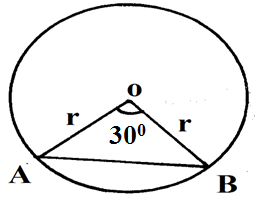
\includegraphics{images/circle.png}

\begin{enumerate}
\def\labelenumi{\arabic{enumi}.}
\setcounter{enumi}{4}
\item
  The curved surface area of a cylindrical container is \(2,112\,cm^2\).
  If the radius of the container is 21cm, calculate to one decimal place
  the capacity of the container in litres \hspace{2.1 cm} \((3mks)\)
\item
  The base of a triangle is 3cm longer than its height. Given that the
  area of the triangle is \(35cm^2\), determine the base of the
  triangle. \hspace{7.2 cm} \((3mks)\)
\item
  A carpenter constructed a closed wooden box with internal measurements
  1.8 m long, 0.8 m wide, and 0.6 m high. The wood used in constructing
  the box was 1.0cm thick and had a density of \(0.75g/cm^{3}\).
  Determine the:

  a) Volume in \(cm^3\) of the wood used in constructing the box.
  \hspace{4.2 cm} \((3mks)\)

  b) Mass of the box in kilograms correct to 4 significant figures.
  \hspace{3.6 cm} \((1mk)\)
\item
  A solid hemisphere of radius 7cm has the same volume as a cube. Find
  the length of the cube to 3 significant figures. \hspace{10.4 cm}
  \((3mks)\)
\item
  Mango juice in a factory is stored in a rectangular tank whose
  internal dimensions are 1.8m by 1.4m by 2.5m one day the tank was 80\%
  full of Mango juice. Calculate the volume of Mango juice in the tank
  in litres. \hspace{10 cm} \((3mks)\)
\item
  An open box has an external breadth of 12 cm, a height 10 cm, and a
  length of 15 cm. If the thickness of the material of the box is 1 cm,
  find the total surface area of the box. \hspace{3.7cm} \((5mks)\)
\item
  A triangular plot PQR is such that the length of the side PQ is
  two-thirds that of QR. The ratio of the lengths \(PQ: PR = 4:9\) and
  the angle at Q is obtuse. If the perimeter of the plot is 38m
  calculate the length of the 3 sides of \(\triangle PQR\)
  \hspace{7.5cm} \((4mks)\)
\item
  A metallic cuboid 10cm by 12cm by 15cm is melted. Half of it is used
  to make a cylinder of radius 4.2cm, the remaining is used to make a
  sphere. Determine in 4 significant figures using \(\pi= \frac{22}{7}\)

  a) The height and surface area of the cylinder to 2 decimal places.
  \hspace{3.2 cm} \((4mks)\)

  b) The radius and surface area of the sphere are correct to 3
  significant figures. \hspace{1.5 cm} \((4mks)\)

  c) The difference between the surface area of the sphere and the
  cylinder. \hspace{1.7cm} \((2mks)\)
\end{enumerate}

\end{tcolorbox}

\bookmarksetup{startatroot}

\chapter{Chapter Eleven: Mass, Weight and
Density}\label{chapter-eleven-mass-weight-and-density}

\bookmarksetup{startatroot}

\chapter*{Mass, Weight and Density}\label{mass-weight-and-density}
\addcontentsline{toc}{chapter}{Mass, Weight and Density}

\markboth{Mass, Weight and Density}{Mass, Weight and Density}

\textbf{Mass}, is the quantity of matter in an object? The Mass of an
object is constant everywhere. Its SI unit is Kilogram (K.g).

\textbf{Weight}, is the pull of the earth on an object. The weight of an
object varies from one place to another on the earth's surface. Its SI
unit is Newton (N). It is given by mass multiplied by the gravitational
force (g).

\(Weight (N) = mass (kg) \times gravity (N/kg).\)

\textbf{Density}, is mass per unit volume. Its SI unit is Kilogram per
Cubic meter (\(kgm^-3\))

\[Density= \frac{mass}{volume}\]
\[Density \,of\, mixture=\frac{mass \,of\, mixture}{volume\, of \,mixture} \]

\begin{tcolorbox}[enhanced jigsaw, left=2mm, colframe=quarto-callout-note-color-frame, toptitle=1mm, opacitybacktitle=0.6, rightrule=.15mm, colbacktitle=quarto-callout-note-color!10!white, colback=white, arc=.35mm, breakable, leftrule=.75mm, bottomtitle=1mm, bottomrule=.15mm, title=\textcolor{quarto-callout-note-color}{\faInfo}\hspace{0.5em}{Conversion of Units}, titlerule=0mm, coltitle=black, toprule=.15mm, opacityback=0]

\begin{equation}
\begin{split}
1 \,tonne &= 1,000\, Kilograms\\
1 \,kilogram &= 1,000 \,grams\\
1g/cm^3& = 1,000 Kg/m^3
\end{split}
\end{equation}

\end{tcolorbox}

\section{Solved Examples}\label{solved-examples-9}

\begin{tcolorbox}[enhanced jigsaw, left=2mm, colframe=quarto-callout-note-color-frame, toptitle=1mm, opacitybacktitle=0.6, rightrule=.15mm, colbacktitle=quarto-callout-note-color!10!white, colback=white, arc=.35mm, breakable, leftrule=.75mm, bottomtitle=1mm, bottomrule=.15mm, title=\textcolor{quarto-callout-note-color}{\faInfo}\hspace{0.5em}{Example 1}, titlerule=0mm, coltitle=black, toprule=.15mm, opacityback=0]

2.5 litres of water of density \(1g/cm^3\) is added to 4 litres of
alcohol of density \(0.8 g/cm^3\). Calculate in 3 significant figures,
the density of the mixture in its SI unit. \hspace{4.2 cm} (3mks)

\end{tcolorbox}

\begin{tcolorbox}[enhanced jigsaw, left=2mm, colframe=quarto-callout-caution-color-frame, toptitle=1mm, opacitybacktitle=0.6, rightrule=.15mm, colbacktitle=quarto-callout-caution-color!10!white, colback=white, arc=.35mm, breakable, leftrule=.75mm, bottomtitle=1mm, bottomrule=.15mm, title=\textcolor{quarto-callout-caution-color}{\faFire}\hspace{0.5em}{Solution}, titlerule=0mm, coltitle=black, toprule=.15mm, opacityback=0]

\[Density \,of \,Mixture (D.M)=\frac{Mass\, of\,mixture}{Volume\, of \,mixture}\]
\[
\begin{aligned}
\text{Volume of water} &= 2,500 \, \text{cm}^3 \\
\text{Mass of water} &= 2,500 \, \text{cm}^3 \times 1 \, \text{g/cm}^3 \\
&= 2,500 \, \text{g} \\
\text{Volume of alcohol} &= 4,000 \, \text{cm}^3 \\
\text{Mass of alcohol} &= 4,000 \, \text{cm}^3 \times 0.8 \, \text{g/cm}^3 \\
&= 3,200 \, \text{g}
\end{aligned}
\]

\[
\begin{aligned}
\text{Mass of Mixture} &= 2,500 \, \text{g} + 3,200 \, \text{g} \\
&= 5,700 \, \text{g} \\
\text{Volume of mixture} &= 2,500 \, \text{cm}^3 + 4,000 \, \text{cm}^3 \\
&= 6,500 \, \text{cm}^3 \\
\therefore \text{Density (D.M.)} &= \frac{5,700}{6,500} \, \text{g/cm}^3 \\
&= 0.8769 \, \text{g/cm}^3 \\
&= 877 \, \text{Kg/m}^3
\end{aligned}
\]

\end{tcolorbox}

\begin{tcolorbox}[enhanced jigsaw, left=2mm, colframe=quarto-callout-note-color-frame, toptitle=1mm, opacitybacktitle=0.6, rightrule=.15mm, colbacktitle=quarto-callout-note-color!10!white, colback=white, arc=.35mm, breakable, leftrule=.75mm, bottomtitle=1mm, bottomrule=.15mm, title=\textcolor{quarto-callout-note-color}{\faInfo}\hspace{0.5em}{Example 2}, titlerule=0mm, coltitle=black, toprule=.15mm, opacityback=0]

wo coils of the same mass are made by winding zinc of different gauges
and lengths. The first coil is made by winding 648 m of wire with a
cross-sectional diameter of 5.4mm and the second coil is made by winding
450 m with different cross-sections. Find the cross-sectional radius of
the second coil. \((3mks)\)

\end{tcolorbox}

\begin{tcolorbox}[enhanced jigsaw, left=2mm, colframe=quarto-callout-caution-color-frame, toptitle=1mm, opacitybacktitle=0.6, rightrule=.15mm, colbacktitle=quarto-callout-caution-color!10!white, colback=white, arc=.35mm, breakable, leftrule=.75mm, bottomtitle=1mm, bottomrule=.15mm, title=\textcolor{quarto-callout-caution-color}{\faFire}\hspace{0.5em}{Solution}, titlerule=0mm, coltitle=black, toprule=.15mm, opacityback=0]

\textbf{Note:} Since mass is proportional to volume for the same
density, the volume of the first coil is equal to volume of the second
coil.

\[
\begin{aligned}
\textbf{First coil volume:} \\
\frac{22}{7} \times \left(\frac{5.4}{2}\right)^2 \times 648,000 &= 14,846,605.71 \, \text{mm}^3 \\
\\
\textbf{Second coil volume:} \\
\frac{22}{7} \times r^2 \times 450,000 &= 1,414,285.714r^2 \, \text{mm}^3 \\
\\
\textbf{Equating second coil volume to first coil volume:} \\
1,414,285.714r^2 &= 14,846,605.71 \, \text{mm}^3 \\
\\
\frac{\cancel{1,414,285.714}r^2}{\cancel{1,414,285.714}} &= \frac{\cancelto{10.4976}{14,846,605.71}}{\cancel{1,414,285.714}} \\
r^2 &= 10.4976 \, \text{mm}^2 \\
\\
\therefore \, r &= 3.24 \, \text{mm}
\end{aligned}
\]

\end{tcolorbox}

\begin{tcolorbox}[enhanced jigsaw, left=2mm, colframe=quarto-callout-note-color-frame, toptitle=1mm, opacitybacktitle=0.6, rightrule=.15mm, colbacktitle=quarto-callout-note-color!10!white, colback=white, arc=.35mm, breakable, leftrule=.75mm, bottomtitle=1mm, bottomrule=.15mm, title=\textcolor{quarto-callout-note-color}{\faInfo}\hspace{0.5em}{Example 3}, titlerule=0mm, coltitle=black, toprule=.15mm, opacityback=0]

The external measurements of a closed metal box are 1.6 m long, 0.7 m
wide, and 0.4 m high. The metal used in making box is 1.0 cm thick and
has a density of 0.85 g/cm3. If the box contains 40 packets of 12
similar tools each and each tool has a mass of 115 g, calculate:

a) The volume of metal used in making the box. \(\hspace{1cm} (4mks)\)

b) The mass of the empty box in Kilograms to 3 significant figures.
\(\hspace{1cm} (3mks)\)

c) The total mass of the box in kilograms to 3 significant figures.
\(\hspace{1cm} (3mks)\)

\end{tcolorbox}

\begin{tcolorbox}[enhanced jigsaw, left=2mm, colframe=quarto-callout-caution-color-frame, toptitle=1mm, opacitybacktitle=0.6, rightrule=.15mm, colbacktitle=quarto-callout-caution-color!10!white, colback=white, arc=.35mm, breakable, leftrule=.75mm, bottomtitle=1mm, bottomrule=.15mm, title=\textcolor{quarto-callout-caution-color}{\faFire}\hspace{0.5em}{Solution}, titlerule=0mm, coltitle=black, toprule=.15mm, opacityback=0]

a)

$$
\begin{aligned}
\textbf{Volume of the Cuboid (v):} & \\
v &= \text{Length} \times \text{Width} \times \text{Height} \\
\textbf{External Measurement:} & \\
\text{Length} &= 160 \, \text{cm} \\
\text{Width} &= 70 \, \text{cm} \\
\text{Height} &= 40 \, \text{cm} \\
\textbf{Internal Measurement:} & \\
\text{Thickness} &= 1 \, \text{cm} \\
\text{Internal Length} &= 158 \, \text{cm} \\
\text{Internal Width} &= 68 \, \text{cm} \\
\text{Internal Height} &= 38 \, \text{cm} \\ 
\end{aligned}
$$

\[
\begin{aligned}
\text{Width} &= 68 \, \text{cm} \\
\text{Height} &= 38 \, \text{cm} \\ 
\textbf{External Volume:} \\
160 \times 70 \times 40 &= 448,000 \, \text{cm}^3 \\ 
\textbf{Internal Volume:} \\
158 \times 68 \times 38 &= 408,272 \, \text{cm}^3 \\ 
448,000 \, \text{cm}^3 - 408,272 \, \text{cm}^3 &= 39,728 \, \text{cm}^3 \\ 
\therefore \textbf{Volume of the metal} &= 39,728 \, \text{cm}^3 
\end{aligned}
\]

b)

\[
\begin{aligned}
\text{Mass} &= \text{density} \times \text{volume} \\
&= 0.85 \, \text{g/cm}^3 \times 39,728 \, \text{cm}^3 \\ 
&= 33,768.8 \, \text{g} \\ 
\frac{33,768.8}{1000} &= 33.7688 \, \text{Kg} \\ 
\therefore \textbf{Mass of the empty box} &= 33.8 \, \text{Kg}
\end{aligned}
\]

c)

\[
\begin{aligned}
\textbf{Mass of tools:} \\
12 \times 40 \times 115 &= 55,200 \, \text{g} \\
\frac{55,200}{1000} &= 55.2 \, \text{Kg} \\
\therefore \textbf{The total Mass} &= 55.2 + 33.8 \\
&= 89.0 \, \text{Kg}
\end{aligned}
\]

\end{tcolorbox}

\begin{tcolorbox}[enhanced jigsaw, left=2mm, colframe=quarto-callout-note-color-frame, toptitle=1mm, opacitybacktitle=0.6, rightrule=.15mm, colbacktitle=quarto-callout-note-color!10!white, colback=white, arc=.35mm, breakable, leftrule=.75mm, bottomtitle=1mm, bottomrule=.15mm, title=\textcolor{quarto-callout-note-color}{\faInfo}\hspace{0.5em}{Problems to Solve}, titlerule=0mm, coltitle=black, toprule=.15mm, opacityback=0]

\begin{enumerate}
\def\labelenumi{\arabic{enumi}.}
\item
  A solid block in the shape of a cylinder has a height of 14cm and
  weighs 26kg. If it is made of material of density \(0.45g/cm^3\), find
  the radius of the cylinder to four significant figures. Take
  \(\pi=\frac{22}{7}\) \hspace{13.7 cm} \((3mks)\)
\item
  \(2000 cm\^3\) of a mixture consists of 2.5 kg of substance x and 7.5
  kg of substance y. find the density of mixture in \(g/cm^3\)
  \hspace{11 cm} \((3mks)\)
\item
  An artisan has 63kg of metal of density \(7g/cm^3\). He intends to use
  it to make a rectangular pipe with external dimensions 12cm by 15cm
  and internal dimensions 10cm by 12 cm. Calculate the length of the
  pipe in metres. \hspace{9.8 cm} \((3mks)\)
\item
  A solid metal cuboid 2.1m long, 0.8m wide, and 0.75m high of material
  of density \(0.75g/cm^3\). Calculate its mass in kilograms.
  \hspace{8.8 cm} \((2mks)\)
\item
  A metal R is an alloy of two metals X and Y. Metal X has a mass of 70g
  and a density of \(16000kg/m^3\). Metal Y has a mass of 42g and a
  density of \(4000 kg/m^3\). In 4 significant figures, calculate the
  density of the metal R in its SI unit. \hspace{6cm} \((4mks)\)
\item
  Two coils of the same mass are made by winding aluminum wire of
  different gauges and lengths. If the first coil is made by winding 540
  m of the wire with diameter 1.96 mm cross-sectional diameter and the
  second coil is made by winding a certain length of the wire with a
  cross-sectional diameter of 2.94 mm, find the length of the second
  coil wire. \hspace{4.3cm} \((3mks)\)
\item
  The external measurements of a wooden box are 1.2 m long, 65 cm wide,
  and 40 cm high. The wood used in making the box is 2 cm thick and has
  a density of \(950 Kg/m^3\). Given that the box contains 30 packets of
  tools and each packet holds a dozen tools each weighing 125 g,
  calculate:

  a) The volume of wood used in making the box. \hspace{6cm} \((4mks)\)

  b) The mass of the empty box in kilograms to four significant figures.
  \hspace{3cm}\((3mks)\)

  c) The total mass of the box in kilograms to 3 significant figures.
  \hspace{3.8cm}\((3mks)\)
\end{enumerate}

\end{tcolorbox}

\bookmarksetup{startatroot}

\chapter{Chapter Twelve: Time}\label{chapter-twelve-time}

\bookmarksetup{startatroot}

\chapter*{Time}\label{time}
\addcontentsline{toc}{chapter}{Time}

\markboth{Time}{Time}

\textbf{Time} can be given in either a 12-hour clock system or a 24-hour
system. In a 12-hour system, time is counted from midnight (12:00
midnight). The time is written as am from midnight to midday and pm from
midday to midnight. In the 24-hour clock system, time is expressed in
hours and counted from midnight to midnight.

To convert a 12-hour clock system to a 24-hour system, add 12 to a pm
time. To convert a 24-hour time to a 12-hour time, subtract 12 if it's
13 or more, then add the right suffix (am if the original value is less
than 13, or pm if the original value is 13 or more).

\begin{tcolorbox}[enhanced jigsaw, left=2mm, colframe=quarto-callout-note-color-frame, toptitle=1mm, opacitybacktitle=0.6, rightrule=.15mm, colbacktitle=quarto-callout-note-color!10!white, colback=white, arc=.35mm, breakable, leftrule=.75mm, bottomtitle=1mm, bottomrule=.15mm, title=\textcolor{quarto-callout-note-color}{\faInfo}\hspace{0.5em}{Problems to Solve}, titlerule=0mm, coltitle=black, toprule=.15mm, opacityback=0]

\begin{enumerate}
\def\labelenumi{\arabic{enumi}.}
\item
  A car left town A for town B at 1000h and had a puncture after
  traveling for 2 h 30 min fixing a new tyre took 36 minutes. The car
  then traveled for another 1 hour 45 min before reaching town B. At
  what time did it arrive? \hspace{9.7 cm} \((3mks)\)
\item
  An airplane left Nairobi at 2045h and arrived in London at 0320h. It
  stayed for \(1\frac{1}{2}\) hours for rest and refreshment of
  passengers and crew. It then headed for Washington D.C and took
  \(9  \frac{1}{4}\) hours.
\end{enumerate}

a) How long did the journey from Nairobi to London take in hours and
minutes? \hspace{0.5 cm} \((2mks)\)

b) At what time did it arrive in Washington D.C.? \hspace{5.6 cm}
\((2mks)\)

\begin{enumerate}
\def\labelenumi{\arabic{enumi}.}
\setcounter{enumi}{2}
\item
  A watch that loses a half-minute every hour was set to read the
  correct time at 0445h on Monday. Determine the time, in the 12-hour
  system, the watch will show on the following Friday at 1845h.
  \hspace{13 cm} \((3mks)\)
\item
  The average lap time for 3 athletes in a long-distance race is 36
  seconds, 40 seconds, and 48 seconds respectively. If they all start
  the race at the same time, find the number of times the slowest runner
  will have been overlapped by the fastest at the time they all cross
  the starting point together again. \hspace{10.7 cm} \((3mks)\)
\item
  The travel timetable below shows the departure and arrival time for a
  bus plying between two towns M and R, 450 kilometers apart.
\end{enumerate}

\begin{center}
    \begin{tabular}{l|c|r} 
      \textbf{TOWN} & \textbf{ARRIVAL} & \textbf{DEPARTURE}\\
      \hline
      M & &0830h \\
      N &       1000h   &       1020h \\
P       &   1310h       &   1340h \\
Q       &   1510h       &   1520h \\
R       &   1600h&         \\

\end{tabular}
\end{center}

\begin{enumerate}
\def\labelenumi{\arabic{enumi}.}
\setcounter{enumi}{5}
\tightlist
\item
  Calculate the average speed for the whole journey. \hspace{7 cm}
  \((3mks)\)
\end{enumerate}

\end{tcolorbox}

\bookmarksetup{startatroot}

\chapter{Chapter 15: Linear
Equations}\label{chapter-15-linear-equations}

\bookmarksetup{startatroot}

\chapter*{Linear Equations}\label{linear-equations}
\addcontentsline{toc}{chapter}{Linear Equations}

\markboth{Linear Equations}{Linear Equations}

Linear equations are equations of straight lines involving one or two
unknown variables. A system of two linear equations forms simultaneous
equations.

There are three methods used to solve simultaneous equations:

\begin{itemize}
\tightlist
\item
  \textbf{Elimination method}
\item
  \textbf{Substitution method}
\item
  \textbf{Graphical method}
\end{itemize}

\section{Solved examples}\label{solved-examples-10}

\subsection{Substitution method}\label{substitution-method}

\begin{tcolorbox}[enhanced jigsaw, left=2mm, colframe=quarto-callout-note-color-frame, toptitle=1mm, opacitybacktitle=0.6, rightrule=.15mm, colbacktitle=quarto-callout-note-color!10!white, colback=white, arc=.35mm, breakable, leftrule=.75mm, bottomtitle=1mm, bottomrule=.15mm, title=\textcolor{quarto-callout-note-color}{\faInfo}\hspace{0.5em}{Example 1}, titlerule=0mm, coltitle=black, toprule=.15mm, opacityback=0]

\begin{align*}
2x - 3y & = -13 \quad \quad \quad (i) \\
y & = 2x + 7 \quad \quad \quad (ii)
\end{align*}

\end{tcolorbox}

\begin{tcolorbox}[enhanced jigsaw, left=2mm, colframe=quarto-callout-caution-color-frame, toptitle=1mm, opacitybacktitle=0.6, rightrule=.15mm, colbacktitle=quarto-callout-caution-color!10!white, colback=white, arc=.35mm, breakable, leftrule=.75mm, bottomtitle=1mm, bottomrule=.15mm, title=\textcolor{quarto-callout-caution-color}{\faFire}\hspace{0.5em}{Solution}, titlerule=0mm, coltitle=black, toprule=.15mm, opacityback=0]

Substituting equation \textbf{(ii)} into \textbf{(i)};

\begin{align*}
  2x - 3(2x + 7) & = -13 \\
  2x - 6x - 21 & = -13 \\
  -4x & = -13 + 21 \\
  \frac{\cancel{-4}x}{\cancel{-4}} & = \frac{\cancelto{-2}{8}}{\cancel{-4}} \\
  x & = -2 
\end{align*}

  \begin{align*}
 but,\, y&=2x+7\\
 Solve\, for\, y:\\
 y&=2(-2)+7\\
 &=3\\ \therefore Solution \,set&=(-2,3)
 \end{align*}

\end{tcolorbox}

\begin{tcolorbox}[enhanced jigsaw, left=2mm, colframe=quarto-callout-note-color-frame, toptitle=1mm, opacitybacktitle=0.6, rightrule=.15mm, colbacktitle=quarto-callout-note-color!10!white, colback=white, arc=.35mm, breakable, leftrule=.75mm, bottomtitle=1mm, bottomrule=.15mm, title=\textcolor{quarto-callout-note-color}{\faInfo}\hspace{0.5em}{Example 2}, titlerule=0mm, coltitle=black, toprule=.15mm, opacityback=0]

\begin{align*}
7x + 15y &= 22...\hspace{2cm} (i)\\
8x + 17y &= 25...\hspace{2cm} (ii)\\
\end{align*}

\end{tcolorbox}

\begin{tcolorbox}[enhanced jigsaw, left=2mm, colframe=quarto-callout-caution-color-frame, toptitle=1mm, opacitybacktitle=0.6, rightrule=.15mm, colbacktitle=quarto-callout-caution-color!10!white, colback=white, arc=.35mm, breakable, leftrule=.75mm, bottomtitle=1mm, bottomrule=.15mm, title=\textcolor{quarto-callout-caution-color}{\faFire}\hspace{0.5em}{Solution}, titlerule=0mm, coltitle=black, toprule=.15mm, opacityback=0]

\begin{align*}
Solving\, for\, x\, in \,(i);\\
x&=\frac{22-15y}{7}\\
substituting \,x=\frac{22-15y}{7} \,in \,(ii)\\
8\left(\frac{22-15y}{7}\right)+17y&=25\\
Multiplying \,both\, side\, by \,7;\\
176-120y+119y&=175\\
\cancel{-}y&=\cancel{-}1\\
y&=1\\ then \, , \,x&=\frac{22-15(1)}{7}\\
&x=1\\
\therefore Solution \,set&=(1,1)
\end{align*}

\end{tcolorbox}

\subsection{Elimination method}\label{elimination-method}

\begin{tcolorbox}[enhanced jigsaw, left=2mm, colframe=quarto-callout-note-color-frame, toptitle=1mm, opacitybacktitle=0.6, rightrule=.15mm, colbacktitle=quarto-callout-note-color!10!white, colback=white, arc=.35mm, breakable, leftrule=.75mm, bottomtitle=1mm, bottomrule=.15mm, title=\textcolor{quarto-callout-note-color}{\faInfo}\hspace{0.5em}{Example 3}, titlerule=0mm, coltitle=black, toprule=.15mm, opacityback=0]

\begin{align*}
3x-7y&=13... \hspace{2cm} (i)\\
6x - 5y& = 8...  \hspace{2.1cm} (ii)
\end{align*}

\end{tcolorbox}

\begin{tcolorbox}[enhanced jigsaw, left=2mm, colframe=quarto-callout-caution-color-frame, toptitle=1mm, opacitybacktitle=0.6, rightrule=.15mm, colbacktitle=quarto-callout-caution-color!10!white, colback=white, arc=.35mm, breakable, leftrule=.75mm, bottomtitle=1mm, bottomrule=.15mm, title=\textcolor{quarto-callout-caution-color}{\faFire}\hspace{0.5em}{Solution}, titlerule=0mm, coltitle=black, toprule=.15mm, opacityback=0]

To eliminate x multiply equation (i) by 2 and (ii) by 1 and then
subtract (ii) from (i);

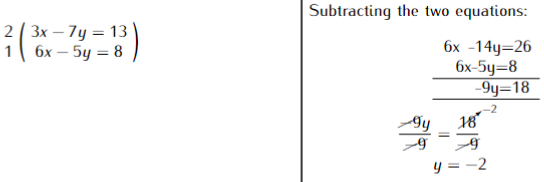
\includegraphics{images/Li_eq_Ex3.png}

Plugging y=-2 in (i) or (ii) to determine the value of x;

\begin{align*}
3x-7(-2)&=13\\
3x+14&=13\\3x&=-1\\
\frac{\cancel{3}x}{\cancel{3}}&=-\frac{1}{3}\\
x&=\frac{-1}{3}\\ Solution\, set&=(-\frac{1}{3},-2)
\end{align*}

\end{tcolorbox}

\begin{tcolorbox}[enhanced jigsaw, left=2mm, colframe=quarto-callout-note-color-frame, toptitle=1mm, opacitybacktitle=0.6, rightrule=.15mm, colbacktitle=quarto-callout-note-color!10!white, colback=white, arc=.35mm, breakable, leftrule=.75mm, bottomtitle=1mm, bottomrule=.15mm, title=\textcolor{quarto-callout-note-color}{\faInfo}\hspace{0.5em}{Example 4 \hspace{11.5 cm} \((4mks)\)}, titlerule=0mm, coltitle=black, toprule=.15mm, opacityback=0]

\[\frac{x+y}{6}-\frac{x+y}{4}=-\frac{1}{4} \]
\[\frac{x-y}{5} + \frac{x-y}{6}=1\frac{1}{10}\]

\end{tcolorbox}

\begin{tcolorbox}[enhanced jigsaw, left=2mm, colframe=quarto-callout-caution-color-frame, toptitle=1mm, opacitybacktitle=0.6, rightrule=.15mm, colbacktitle=quarto-callout-caution-color!10!white, colback=white, arc=.35mm, breakable, leftrule=.75mm, bottomtitle=1mm, bottomrule=.15mm, title=\textcolor{quarto-callout-caution-color}{\faFire}\hspace{0.5em}{Solution}, titlerule=0mm, coltitle=black, toprule=.15mm, opacityback=0]

Simplifying the two equations;

Multiply the 1st equation by 12;

\[\left(\frac{x+y}{6}-\frac{x+y}{4}=\frac{-1}{4}\right)12\]
\[2x+2y-3x-3y=-3\] \[-x-y=-3 \,\ldots \ldots\ldots(i)\]

Multiply the 2nd equation by 30;

\[\left(\frac{x-y}{5}+\frac{x-y}{6}=\frac{11}{10}\right)30\]
\[6x-6y+5x-5y=33\]

\[11x-11y=33 \, \ldots\ldots\ldots (ii)\]

Multiply equation (i) by 11 and add to equation (ii) to eliminate x;

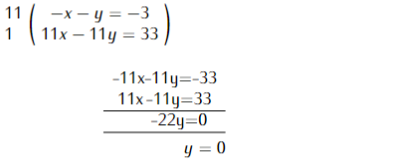
\includegraphics{images/Li_eq_Ex4.png}

Plugging \(y= 0\) in (i) or (ii) to determine the value of x;

\begin{align*}
-x-y(0)&=-3\\
-x&=-3\\x&=3\\
\therefore Solution \,set&=(3,0)
\end{align*}

\end{tcolorbox}

\begin{tcolorbox}[enhanced jigsaw, left=2mm, colframe=quarto-callout-note-color-frame, toptitle=1mm, opacitybacktitle=0.6, rightrule=.15mm, colbacktitle=quarto-callout-note-color!10!white, colback=white, arc=.35mm, breakable, leftrule=.75mm, bottomtitle=1mm, bottomrule=.15mm, title=\textcolor{quarto-callout-note-color}{\faInfo}\hspace{0.5em}{Problems to Solve}, titlerule=0mm, coltitle=black, toprule=.15mm, opacityback=0]

\begin{enumerate}
\def\labelenumi{\arabic{enumi}.}
\tightlist
\item
  Solve the following equations \hspace{9.5 cm} \((4mks)\)
\end{enumerate}

\begin{equation}
\begin{split}
\frac{3y-2x}{15}+\frac{2x+1}{3}&=2\\
\frac{2x-3y}{15}-\frac{1-x}{3}&=1
\end{split}
\end{equation}

\begin{enumerate}
\def\labelenumi{\arabic{enumi}.}
\setcounter{enumi}{1}
\tightlist
\item
  Solve the simultaneous equations. \hspace{8.7 cm} \((3mks)\)
\end{enumerate}

    \begin{align*}
    2x+3y &= 4\\
    x + 4y &= 7
    \end{align*}

\begin{enumerate}
\def\labelenumi{\arabic{enumi}.}
\setcounter{enumi}{2}
\tightlist
\item
  Solve the simultaneous equations: \hspace{8.5 cm} \((3mks)\)
\end{enumerate}

\begin{align*}
2x -y+ 2 &= 0 \\
-3y + x &= -6 
\end{align*}

\begin{enumerate}
\def\labelenumi{\arabic{enumi}.}
\setcounter{enumi}{3}
\item
  Mercy a student at Mucagara mixed Secondary bought 5 pens and 3
  exercise books from Magunas supermarket at Ksh. 135, at the same time
  Murugi her class mate also bought 4 pens and 5 exercise books and
  spent Ksh. 25 more than Mercy. Find the cost of each pen and exercise
  book. \hspace{13.2 cm} \((4mks)\)
\item
  In July, Kiama donated \(\frac{1}{6}\)th of his salary to a children's
  home while Joshua donated \(\frac{1}{5}\)th of his salary to the same
  children's home. Their total donation for July was \(Ksh.\, 14,820\).
  In August, Kiama donated \(\frac{1}{8}\)th of his salary to the
  children's home while Joshua donated \(\frac{1}{12}\)th of his salary
  to the children's home. Their total donation for August was
  \(Ksh.\, 8,675\). Calculate Kiama's monthly salary. \hspace{13.1 cm}
  \((4mks)\)
\item
  Three spoons and four plates cost \(Ksh. \,87\). Two spoons and five
  plates cost \(Ksh.\, 93\). Find the cost of one spoon and one plate.
  \hspace{9cm} \((4mks)\)
\item
  Mwendia bought 8 pairs of trousers and six socks at \(Ksh.\, 4,160\).
  Had he bought twice as many socks and half as many trousers, he would
  have saved \(Ksh.\, 100\). Find the cost of each item. \hspace{14.3cm}
  \((3mks)\)
\item
  Esther bought 144 mangoes at \(Ksh.\, 100\) for every six mangoes. She
  sold some of them at \(Ksh.\, 72\) for every three and the rest at
  \(Ksh.\, 60\) for every two. If she made a 45\% profit, calculate the
  number of mangoes sold at \(Ksh.\, 72\) for every three.
  \hspace{7.1cm} \((3mks)\)
\item
  Four men took their cows to the market. John had two more cows than
  Enoch. Alex had as many cows as John, whereas Jeff had 10 cows less
  than the sum of both John and Alex.

  a) Write a simplified expression with one variable, representing the
  total number of cows. \hspace{13.6cm} \((1mk)\)

  b) Three butchers bought all the cows and shared them equally. If each
  butcher got 17 cows, how many did Jeff sell to the butchers
  \hspace{7.5 cm} \((3mks)\)
\item
  Wanjiru bought three cups and four plates for Ksh. 324. Moraa bought
  five cups and Anyango bought two plates of the same type as those
  bought by Wanjiru. Moraa paid \(Ksh.\, 228\) more than Anyango. Find
  the price of each cup and spoon. \hspace{5.4cm} \((3mks)\)
\item
  Daniel and Sokoro bought the same types of pens and blades from the
  same shop. Daniel bought 2 pens and 3 blades for \(Ksh.\, 78\). Sokoro
  bought 3 pens and 4 blades and spent \(Ksh.\, 36\) more than Daniel.
  Calculate the cost of each item \hspace{6cm} \((3mks)\)
\item
  Karani bought 4 pencils and 6 blades for \(Ksh.\, 66\) and Kanuni
  bought 2 pencils and 5 blades for \(Ksh.\, 51\).

  a) Find the price of each item.\hspace{9cm} \((3mks)\)

  b) Naomi spent Ksh. 228 to buy the same type of pencils and blades. If
  the number of blades she bought was 4 more than the number of pencils,
  find the number of pencils bought. \hspace{13.5cm} \((3mks)\)
\item
  A retailer bought 50 plates and 30 spoons from a wholesaler P for
  \(Ksh.\, 4260\). Had she bought 15 plates less and half spoons more,
  she would have paid \(Ksh. \,990\) less. Had the retailer bought from
  wholesaler Q, she would have paid 50\% more for a plate and 25\% less
  for a spoon. How much would she have lost if she had bought the 50
  plates and the 30 spoons from wholesaler Q.? \hspace{14.2 cm}
  \((10mks)\)
\end{enumerate}

\end{tcolorbox}

\bookmarksetup{startatroot}

\chapter{Chapter Fourteen: Commercial
Arithmetic}\label{chapter-fourteen-commercial-arithmetic}

\bookmarksetup{startatroot}

\chapter*{Commercial Arithmetic}\label{commercial-arithmetic}
\addcontentsline{toc}{chapter}{Commercial Arithmetic}

\markboth{Commercial Arithmetic}{Commercial Arithmetic}

Currency is the medium of any business transaction. In Kenya, shillings
are used as the basic currency unit. 1 Kenyan shilling \((Ksh)\) is
equal to 100 cents \((ct)\).

\section{Solved Examples}\label{solved-examples-11}

\begin{tcolorbox}[enhanced jigsaw, left=2mm, colframe=quarto-callout-note-color-frame, toptitle=1mm, opacitybacktitle=0.6, rightrule=.15mm, colbacktitle=quarto-callout-note-color!10!white, colback=white, arc=.35mm, breakable, leftrule=.75mm, bottomtitle=1mm, bottomrule=.15mm, title=\textcolor{quarto-callout-note-color}{\faInfo}\hspace{0.5em}{Example 1}, titlerule=0mm, coltitle=black, toprule=.15mm, opacityback=0]

Use the exchange rates below to answer this question. \hspace{6cm}
\((3mks)\)

\(\hspace{5.1cm} Buying\hspace{2.9cm} Selling\)

1 US dollar \(\hspace{3.3cm}102.20 \hspace{3cm} 102.80\)

1 UK £ \(\hspace{4cm}132.30 \hspace{3cm} 132.95\)

A European tourist arriving in Kenya from Britain had 12,600 UK Sterling
pounds (£). He converted the pounds to Kenya shillings at a commission
of 5\%. While in Kenya, he spent \(\frac{4}{5}\) of this money. He
changed the balance to US dollars after his stay. If he was not charged
any commission for this last transaction, calculate to the nearest US
dollars, the amount he received.

\end{tcolorbox}

\begin{tcolorbox}[enhanced jigsaw, left=2mm, colframe=quarto-callout-caution-color-frame, toptitle=1mm, opacitybacktitle=0.6, rightrule=.15mm, colbacktitle=quarto-callout-caution-color!10!white, colback=white, arc=.35mm, breakable, leftrule=.75mm, bottomtitle=1mm, bottomrule=.15mm, title=\textcolor{quarto-callout-caution-color}{\faFire}\hspace{0.5em}{Solution}, titlerule=0mm, coltitle=black, toprule=.15mm, opacityback=0]

To Convert foreign currency to Kenyan currency, the bank Buys from you
(use the Buying column. But, from Kenyan currency to foreign currency,
the bank sells to you (use the Selling column)

\begin{align*}
He\, received &=12,500 \times 132.30 \\&=Ksh. 1,666,980\\
After \,commission,\, he \,gets:\\ &= \frac{95}{100}\times 1,666,980\\&=1,583,631\\
\end{align*}

Balance after spending \(\frac{4}{5}\) of his money:

 \begin{align*}
 &=\frac{1}{5}\times 1,583,631\\&=Ksh.\, 237,667.20 \\US\, dollars\, he\, received: \\
&=\frac{237,667.20}{102.80}\\&=2,311.94\\
 \therefore He \,received: \,2,312 \,US \,dollars 
\end{align*}

\end{tcolorbox}

\begin{tcolorbox}[enhanced jigsaw, left=2mm, colframe=quarto-callout-note-color-frame, toptitle=1mm, opacitybacktitle=0.6, rightrule=.15mm, colbacktitle=quarto-callout-note-color!10!white, colback=white, arc=.35mm, breakable, leftrule=.75mm, bottomtitle=1mm, bottomrule=.15mm, title=\textcolor{quarto-callout-note-color}{\faInfo}\hspace{0.5em}{Example 2}, titlerule=0mm, coltitle=black, toprule=.15mm, opacityback=0]

A Kenyan bank buys and sells foreign currencies at the exchange rates
shown below.

\(\hspace{5.1cm} BUYING \,(KSH) \hspace{2.6cm} SELLING \,(KSH)\)

1Euro \(\hspace{4.4cm} 147.56 \hspace{4.6cm} 148.00\)

1U.S Dollar \(\hspace{3.5cm} 102.22 \hspace{4.6cm} 102.50\)

A foreign woman arrived in Kenya with 25,000 Euros. He converted all the
Euros into Kenyan Shillings at the bank. He spent \(Ksh.\, 2, 610,200\)
while in Kenya and converted the remaining Kenya shillings into U.S
Dollars at the bank. Calculate to the nearest dollars the amount that
she received. \hspace{15.2cm} \((3mks)\)

\end{tcolorbox}

\begin{tcolorbox}[enhanced jigsaw, left=2mm, colframe=quarto-callout-caution-color-frame, toptitle=1mm, opacitybacktitle=0.6, rightrule=.15mm, colbacktitle=quarto-callout-caution-color!10!white, colback=white, arc=.35mm, breakable, leftrule=.75mm, bottomtitle=1mm, bottomrule=.15mm, title=\textcolor{quarto-callout-caution-color}{\faFire}\hspace{0.5em}{Solution}, titlerule=0mm, coltitle=black, toprule=.15mm, opacityback=0]

\begin{align*}
She\, received&=25000\times 147.56\\&=Ksh. 3,689,000\\ Balance \,after \,spending:\\
&= 3,689,000-2, 610,200\\&=Ksh. 1,078,800\\
  US \,dollars \,she \,received:\\
&=\frac{1,078,800}{102.5}\\
&=10,524.88\\ \therefore \,She\, received: \,&10,525 \,US \,dollars
\end{align*}

\end{tcolorbox}

\begin{tcolorbox}[enhanced jigsaw, left=2mm, colframe=quarto-callout-note-color-frame, toptitle=1mm, opacitybacktitle=0.6, rightrule=.15mm, colbacktitle=quarto-callout-note-color!10!white, colback=white, arc=.35mm, breakable, leftrule=.75mm, bottomtitle=1mm, bottomrule=.15mm, title=\textcolor{quarto-callout-note-color}{\faInfo}\hspace{0.5em}{Example 3}, titlerule=0mm, coltitle=black, toprule=.15mm, opacityback=0]

Mr.~Albert who deals in electronics sells a radio to a customer at
\(Ksh.\, 1,350\) after giving him a discount of 10\% but finds that he
still makes a 20\% profit. Find the percentage profit Mr.~Albert would
make if he does not give a discount. \hspace{11cm} \((3mks)\)

\end{tcolorbox}

\begin{tcolorbox}[enhanced jigsaw, left=2mm, colframe=quarto-callout-caution-color-frame, toptitle=1mm, opacitybacktitle=0.6, rightrule=.15mm, colbacktitle=quarto-callout-caution-color!10!white, colback=white, arc=.35mm, breakable, leftrule=.75mm, bottomtitle=1mm, bottomrule=.15mm, title=\textcolor{quarto-callout-caution-color}{\faFire}\hspace{0.5em}{Solution}, titlerule=0mm, coltitle=black, toprule=.15mm, opacityback=0]

\(\textbf{Note:}\) The marked price and the Buying Price (B.P) are
always 100\%

Marked Price (M.P) of the radio:

\begin{align*}
\frac{1350\times 10\cancel{0}}{9\cancel{0}}&=Ksh.\: 1,500 \\Buying\, Price (B.P):\\ \frac{1,35\cancel{0}\times 100}{12\cancel{0}}&=Ksh. \:1,125
\end{align*}

Profit gained if no discount was offered:

\begin{align*}
1,500-1,125&=Ksh. \:375
\end{align*}

Percentage profit (P.P):

\begin{align*}
&=\left(\frac{profit}{B.P}\right)\times 100\\
P.P&=\frac{375}{1,125}\times 100\\&=33.33\%
\end{align*}

\(\therefore\) He would make \(33\frac{1}{3}\%\) profit

\end{tcolorbox}

\begin{tcolorbox}[enhanced jigsaw, left=2mm, colframe=quarto-callout-note-color-frame, toptitle=1mm, opacitybacktitle=0.6, rightrule=.15mm, colbacktitle=quarto-callout-note-color!10!white, colback=white, arc=.35mm, breakable, leftrule=.75mm, bottomtitle=1mm, bottomrule=.15mm, title=\textcolor{quarto-callout-note-color}{\faInfo}\hspace{0.5em}{Example 4}, titlerule=0mm, coltitle=black, toprule=.15mm, opacityback=0]

Judy bought some rice at the wholesale price of \(Ksh.\, 65\) per kg.
She packed three-fifths of the rice in 2 kg bags and sold each bag at
\(Ksh.\, 160\). She packed the remaining in 1 kg bags and sold each bag
at \(Ksh.\, 85\). After selling all the rice she found that she had made
a profit of \(Ksh. \, 6460\).

a) Calculate the amount of rice she bought \hspace{8cm} \((6mks)\)

b) In three significant figures, determine:

i) The percentage profit she made. \hspace{8.2cm} \((2mks)\)

ii) The percentage profit he would have made if sold all the rice in 2
kg bags. \hspace{1.5cm} \((2mks)\)

\end{tcolorbox}

\begin{tcolorbox}[enhanced jigsaw, left=2mm, colframe=quarto-callout-caution-color-frame, toptitle=1mm, opacitybacktitle=0.6, rightrule=.15mm, colbacktitle=quarto-callout-caution-color!10!white, colback=white, arc=.35mm, breakable, leftrule=.75mm, bottomtitle=1mm, bottomrule=.15mm, title=\textcolor{quarto-callout-caution-color}{\faFire}\hspace{0.5em}{Solution}, titlerule=0mm, coltitle=black, toprule=.15mm, opacityback=0]

a)

Let the amount of rice be \(x\)

\begin{align*}
2Kg \,bags&=\frac{3}{5}x
\end{align*}

Selling price (S.P) for 2kg bags:

\begin{align*}
 &=\left(\frac{3}{5}x\right)\frac{160}{2}\\
 &=48x\\ 1Kg\, bags&=x-\frac{3}{5}x\\&=\frac{2}{5}x
 \end{align*}

Selling price for 1Kg bags:

\begin{align*}
&=\frac{2}{5}x\times 85\\&=34x\\
Total \,selling \,price&=48x+34x\\&=82x
\end{align*}

Buying Price (B.P) of the rice:

\begin{align*}
&=65x\\
Profit&=S.P-B.P\\ 82x-65x&=6460 \\ \frac{\cancel{17}x}{\cancel{17}}&=\frac{\cancelto{380}{6460}}{\cancel{17}}\\&=380\\
\therefore The \,amount \,of \,Rice &=380 \,kg
\end{align*}

b) i)

\begin{align*}
Percentage\, profit (p.p)&=\frac{profit}{B.p}\times 100\\
B.p&=380\times 65\\&=24700\\
&=\left(\frac{6460}{247\cancel{00}}\right)\cancel{100}\\
&\approx 26.154\%\\
\therefore p.p&= 26.2\%
\end{align*}

ii)

\begin{align*}
S.p&=\left(\frac{380}{2}\right)160\\&=30400\\
profit&=30,400-24,700\\&=5700\\
p.p&=\left(\frac{5700}{247\cancel{00}}\right)\cancel{100}\\ &\approx23.077\%\\
\therefore p.p&= 23.1\%
\end{align*}

\end{tcolorbox}

\begin{tcolorbox}[enhanced jigsaw, left=2mm, colframe=quarto-callout-note-color-frame, toptitle=1mm, opacitybacktitle=0.6, rightrule=.15mm, colbacktitle=quarto-callout-note-color!10!white, colback=white, arc=.35mm, breakable, leftrule=.75mm, bottomtitle=1mm, bottomrule=.15mm, title=\textcolor{quarto-callout-note-color}{\faInfo}\hspace{0.5em}{Problems to solve}, titlerule=0mm, coltitle=black, toprule=.15mm, opacityback=0]

\begin{enumerate}
\def\labelenumi{\arabic{enumi}.}
\tightlist
\item
  A Kenya bank buys and sells foreign currencies as shown
\end{enumerate}

\(\hspace{5.1cm} Buying \,(Ksh) \hspace{2.3cm}Selling \,(Ksh)\)

1Euro \(\hspace{4cm} 116.26 \hspace{3.8cm} 116.80\)

100 Japanese Yen \(\hspace{2.2cm} 91.36 \hspace{4cm} 91.45\)

A Japanese traveling from France to Kenya had 5,000 Euros. He converted
all the 5,000 Euros to Kenya shillings at the bank. While in Kenya, he
spent a total of \(Ksh.\, 389,850\) and then converted the remaining
Kenya shilling to Japanese Yens at the bank. Calculate the amount in
Japanese Yen that he received. \hspace{9.1cm} \((3mks)\)

\begin{enumerate}
\def\labelenumi{\arabic{enumi}.}
\setcounter{enumi}{1}
\tightlist
\item
  A Kenyan bank buys and sells foreign currency as shown below.
\end{enumerate}

\(\hspace{4.7cm} Buying \,(Ksh)\hspace{2.3cm} Selling \,(Ksh)\)

1 Euro \(\hspace{3.8cm}116.15 \hspace{3.5cm} 116.26\)

1 US Dollar \(\hspace{2.9cm}100.43 \hspace{3.5cm} 100.80\)

A foreigner traveling from Britain arrives in Kenya with 6,500 Euros. He
converts all the Euros to Kenya shillings at the bank. While in Kenya he
spends a total of \(KSh.\, 459,650\) and then converts the remaining
Kenya shillings to US dollars at the bank. Calculate (to the nearest
dollar) the amount he receives. \hspace{10.2cm } \((3mks)\)

\begin{enumerate}
\def\labelenumi{\arabic{enumi}.}
\setcounter{enumi}{2}
\tightlist
\item
  A forex bureau buys and sells American dollars in Kenya shillings at
  the rate shown below.
\end{enumerate}

\(\hspace{2cm} Buying\hspace{3.5cm} Selling\)

\(\hspace{2.3cm} 102.40 \hspace{3.7cm}102.81\)

An American woman at the end of her tour in Kenya had \(Ksh. \,107,500\)
which he converted to the dollar through the Forex bureau. How many
dollars did she get? \hspace{3.3cm}\((2mks)\)

\begin{enumerate}
\def\labelenumi{\arabic{enumi}.}
\setcounter{enumi}{3}
\item
  A tourist arrived from Los Angeles and changed his US Dollar 3,650 to
  \(Ksh.\) He spent \(Ksh. \, 3,000\) per night in a hotel for 20 nights
  and a further \(Ksh. \, 9,000\) daily for the entire period. He left
  for South Africa having changed the balance to South African Rand.
  Calculate the amount of South African Rands he left with, if the bank
  buys and sells currencies using the table below. \hspace{14.3cm}
  \((3mks)\)

  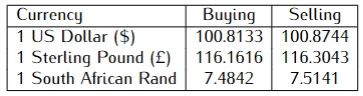
\includegraphics{Cpt14_Q4.png}
\item
  Kavula sold a bag of potatoes for \(Ksh.\, 420\) and made a profit. If
  she sold it at \(Ksh. \,320\), she could have made a loss. Given that
  the profit is thrice the loss, how much did she pay for the bag of
  potatoes? \hspace{11.4cm} \((3mks)\)
\item
  The marked price of a Toyota car in a dealer's shop was
  \(Ksh. \, 450,000\). Tom bought the car at 7\% discount. The dealer
  still made a profit of 13\%. Calculate the amount of money the dealer
  had paid for the car. \hspace{11.4cm} \((3mks)\)
\item
  A 6kg gas cylinder was bought at \(Ksh.\,2,250\) and then later sold
  for \(Ksh.\,2,790\). Calculate:-

  a) The percentage profit. \hspace{9.6cm} \((2mks)\)

  b) The price at which it should be sold to make a profit of 28\%.
  \hspace{3.5cm}\((2mks)\)
\item
  Mwikali paid \(Ksh. 160\) for a blouse after getting a discount of
  20\%.The vendor made a profit of 25\% on the sale of this blouse. What
  percentage profit would the vendor have made if no discount was
  allowed? \hspace{12.1cm} \((3mks)\)
\item
  Mr.~Nyamu who deals in computer accessories sells a laptop to a
  customer at \(Ksh.\, 21,500\) after giving him a discount of 10\% but
  finds that he still makes a 25\% profit. Find the profit Mr.Nyamu
  would make if he does not give a discount. \hspace{7.1cm} \((3mks)\)
\item
  The marked price of a pro-box in a dealer's shop was
  \(Ksh.\, 850,000\). Mucai bought the car at 8\% discount. The dealer
  still made a profit of 15\%. Calculate the amount of money the dealer
  had paid for the car. \hspace{10.8cm} \((3mks)\)
\end{enumerate}

\begin{enumerate}
\def\labelenumi{\arabic{enumi}.}
\setcounter{enumi}{10}
\item
  An electronic company imported into the country some speakers that
  cost \(Ksh.\, 25,750\) each. The government imposed an import duty of
  20\% and a sales tax of 15\%. If the company decides to make a 20\%
  profit on sales, calculate to the nearest shillings the selling price
  of each speaker. \hspace{14.2cm} \((4mks)\)
\item
  A manufacturer sells an empty crate of soda to a trader at a profit of
  50\%. The trader sells it for \(Ksh.\, 360\) at a profit of 20\%. Find

  a) The trader's buying price. \hspace{9cm} \((2mks)\)

  The cost of manufacture of an empty crate. \hspace{6cm} \((3mks)\)
\item
  A Kenyan tradesman owes US \$ 180,000 to a company in the United
  States of America. The Kenyan can either pay through his account in
  Kenya or through his account in the United Kingdom. Which method is
  cheaper and by how much? (Give your answer in Kenyan shillings given
  that: \hspace{12.3cm} \((4mks)\)
\end{enumerate}

\(\hspace{1cm} 1\, US \,dollar \,= 102.74\, Kenyan \,shillings.\)

\(\hspace{1cm} 1 \,Sterling \,pound = 1.79 \,US \,dollar\)

\(\hspace{1cm} 1\, Sterling \,pound = 132.87 \,Kenyan\, shillings\)

\begin{enumerate}
\def\labelenumi{\arabic{enumi}.}
\setcounter{enumi}{13}
\tightlist
\item
  A Forex Bureau in Kenya buys and sells foreign currencies as shown
  below:
\end{enumerate}

\(\hspace{4cm} Buying\, (Ksh) \hspace{2.7cm} Selling \, Ksh)\)

Chinese Yuan \(\hspace{2cm} 15.34 \hspace{4cm} 15.58\)

South African Rand \(\hspace{1cm} 11.28 \hspace{4cm} 11.45\)

A merchant from China converted 205,250 Chinese Yuan into Kenya
Shillings.

\begin{enumerate}
\def\labelenumi{\alph{enumi})}
\item
  Calculate the amount of Money, in Kenya shillings, that she received.
  \hspace{2cm} \((1mk)\)
\item
  While in Kenya, the merchant spent \(Ksh.\, 1,858,000\) and then
  converted the balance to South African Rand. Calculate the amount of
  money, to the nearest Rand, that he received. \hspace{13.5cm}
  \((3mks)\)
\end{enumerate}

\begin{enumerate}
\def\labelenumi{\arabic{enumi}.}
\setcounter{enumi}{14}
\item
  A vehicle sales agent is paid a commission on all vehicles bought
  through him. During a certain month, he sold 2 cars at
  \(Ksh. 1.5 \,million\) each, 5 probox at \(Ksh.\, 650,000\) each and 5
  vans at \(Ksh.\, 1.8 \,million\) each. If he was paid a total
  commission of \(Ksh.\, 720,000\), calculate the percentage rate of
  commission he was paid in 3 significant figures. \hspace{6.8cm}
  \((3mks)\)
\item
  Kang'ethe bought a pair of shoes for \(Ksh.\, 1,600\) and marked it at
  a price such that after allowing his customer a 20\% discount, he
  would make a profit of 25\%. Calculate the marked price of the shoes.
  \hspace{13.1cm} \((4mks)\)
\item
  Muringo bought a skirt at \(Ksh.\, 600\) and marked it at a price such
  that after allowing her customer a 5\% discount she would make a
  profit of 33\%. Find the marked price of the skirt. \hspace{14.3cm}
  \((4mks)\)
\item
  Noah sold a second-hand computer which was marked at \(Ksh. 24,000\)
  to a customer at 19\% discount. If he still made a 20\% profit on the
  cost price, what was its cost price? \hspace{3cm} \((4mks)\)
\item
  A businessman sold a pair of shoes which was marked at
  \(Ksh.\, 2,700\) to a customer allowing a 15\% discount. If he still
  made a 35\% profit on the cost price, determine how much he had paid
  for the pair of shoes. \hspace{12cm} \((4mks)\)
\item
  The marked price of a second-hand car was \(Ksh.\, 625,000\). Mwendia
  sold the car at a discount of 7.2\% and received \(Ksh.\, 49,300\) as
  a commission of the sale. Calculate the percentage rate of commission
  he was paid. \hspace{10.3cm}\((3mks)\)
\item
  Three partners Ndirangu, Isa, and Mukami contributed
  \(Ksh. \,700,000\), \(Ksh.\, 500,000\) and \(Ksh.\, 900,000\)
  respectively to start a business of a mini-bus plying the Embu--
  Nairobi route. The mini-bus carries 25 passengers with each paying
  \(Ksh.\, 250\). The mini-bus makes two round trips each day and ever
  full. Each day \(Ksh.\, 8,000\) is used to cover running costs and
  wages.

  a) Calculate their net profit per day. \hspace{7.6cm} \((2mks)\)

  b) The matatu works for 25 days per month and is serviced every month
  at a cost of \(Ksh.\,12, 000\). Calculate their monthly in July.
  \hspace{6.4cm} \((1mk)\)

  c) The three partners agreed to save 42\% of the profit, 75\% of the
  remainder to be shared in the ratio of their contribution. Calculate
  Mukami's share in the month of July. \hspace{1.8cm} \((4mks)\)

  d) The mini-bus developed mechanical problems and they decided to sell
  it through an agent who charged a commission of 5\% on the selling
  price. Each partner received \(Ksh.\, 520,000\) from the agent after
  he had taken his commission. Determine the price at which the agent
  sold the matatu. \hspace{11.25cm} \((3mks)\)
\item
  Wangari bought some sugar at \(Ksh.\, 80\) per kg. She packed
  five-eighths of the sugar in \(\frac {1}{2}\) kg packets which she
  sold at \(Ksh.\, 60\) per packet. She packed the remaining sugar in 1
  kg packets and sold them at \(Ksh.\, 110\) per packet. She sold all
  the sugar in this way and made a profit of \(Ksh.\, 10,875\).

  a) Determine the amount of sugar she bought. \hspace{6.5cm}\((4mks)\)

  b) Calculate to one decimal place:

  c)

  i) The percentage profit she made. \hspace{7.3cm} \((3mks)\)

  ii) The percentage profit she would have made if she had sold all the
  sugar at \(\frac{1}{2}\) kg packets. \hspace{12.8cm} \((3mks)\)
\item
  A manufacturer made a mattress and sold it to a wholesaler at a profit
  of 25\%. The wholesaler sold the mattress to a shopkeeper at a profit
  of 32\%. The shopkeeper finally sold the mattress to a customer at
  50\% profit.

  a) Determine how much a customer paid for the mattress that had cost
  the manufacturer \(Ksh.\, 1800\) to make. \hspace{11cm} \((3mks)\)

  b) A customer paid \(Ksh.\, 3,465\) for another mattress. Determine
  how much it had cost the manufacturer to make the mattress.
  \hspace{8.2cm} \((3mks)\)

  c) The shopkeeper bought the mattress which had cost the wholesaler
  \(Ksh.\, 3,500\). He marked the mattress at a price such that after
  allowing his customer a discount of 10\%, he would still make a profit
  of 50\%. Find the price at which the mattress was marked.\hspace{1cm}
  \((4mks)\)
\end{enumerate}

\end{tcolorbox}

\bookmarksetup{startatroot}

\chapter{Chapter Fifteen: Co-Ordinates and
Graphs}\label{chapter-fifteen-co-ordinates-and-graphs}

\bookmarksetup{startatroot}

\chapter*{Co-Ordinates and Graphs}\label{co-ordinates-and-graphs}
\addcontentsline{toc}{chapter}{Co-Ordinates and Graphs}

\markboth{Co-Ordinates and Graphs}{Co-Ordinates and Graphs}

A coordinate is an ordered pair of numbers used to locate the position
of a point in a plane and written in the form (x, y). The first number,
x represents the distance along the x-axis and it is called x the
coordinate. The second number, y represents the distance along the
y-axis and it is called the y coordinate.

The x and y axes divide the plane into four regions and each region is
called a \textbf{quadrant}. The quadrants are named 1st quadrant, 2nd
quadrant, 3rd quadrant, and 4th quadrant starting with the top
right-hand quadrant and moving in anti-clockwise direction.

\textbf{Rectangular Cartesian co-ordinate system} is a system of
locating points using two axes at right angles.

We can also use coordinate systems such as latitude and longitudes and
grid references to locate places on the earth's surface.

\section{Solved Examples}\label{solved-examples-12}

\begin{tcolorbox}[enhanced jigsaw, left=2mm, colframe=quarto-callout-note-color-frame, toptitle=1mm, opacitybacktitle=0.6, rightrule=.15mm, colbacktitle=quarto-callout-note-color!10!white, colback=white, arc=.35mm, breakable, leftrule=.75mm, bottomtitle=1mm, bottomrule=.15mm, title=\textcolor{quarto-callout-note-color}{\faInfo}\hspace{0.5em}{Example 1}, titlerule=0mm, coltitle=black, toprule=.15mm, opacityback=0]

A certain quantity of gas is heated from \(0\,^{\circ}\mathrm{C}\), and
the volume is measured at different temperatures. The table below gives
the corresponding values:

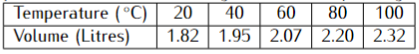
\includegraphics{images/Cpt15_Ex1.png}

a) Draw a graph of volume against temperature using a suitable scale.

b) Use your graph to find:

i) The initial volume of the gas

ii) The volume of the gas when the temperature is
\(50\,^{\circ}\mathrm{C}\) and \(64\,^{\circ}\mathrm{C}\)

iii) The temperature of the gas when the volume is 1.9 litres and 2.3
litres.

\end{tcolorbox}

\begin{tcolorbox}[enhanced jigsaw, left=2mm, colframe=quarto-callout-caution-color-frame, toptitle=1mm, opacitybacktitle=0.6, rightrule=.15mm, colbacktitle=quarto-callout-caution-color!10!white, colback=white, arc=.35mm, breakable, leftrule=.75mm, bottomtitle=1mm, bottomrule=.15mm, title=\textcolor{quarto-callout-caution-color}{\faFire}\hspace{0.5em}{Solution}, titlerule=0mm, coltitle=black, toprule=.15mm, opacityback=0]

a) The graph is depicted in the figure 15.1:

\begin{figure}[H]

{\centering \includegraphics{Co-Ordinates-and-Graphs_files/figure-pdf/unnamed-chunk-1-1.pdf}

}

\caption{The Graph of Volume against Temperature}

\end{figure}%

\b)

i) The initial volume is obtained by extrapolating the line to cut the
y-axis. Therefore the initial volume is 1.7 litres.

ii) The volume of the gas at \(50\,^{\circ}\mathrm{C}\) is 2 litres

The volume of the gas at \(64\,^{\circ}\mathrm{C}\) is 2.1 litres.

iii) The temperature of the gas at 1.9 litres is
\(35\,^{\circ}\mathrm{C}\)

The temperature of the gas at 2.3 litres is \(98\,^{\circ}\mathrm{C}\)

\end{tcolorbox}

\begin{tcolorbox}[enhanced jigsaw, left=2mm, colframe=quarto-callout-note-color-frame, toptitle=1mm, opacitybacktitle=0.6, rightrule=.15mm, colbacktitle=quarto-callout-note-color!10!white, colback=white, arc=.35mm, breakable, leftrule=.75mm, bottomtitle=1mm, bottomrule=.15mm, title=\textcolor{quarto-callout-note-color}{\faInfo}\hspace{0.5em}{Example 2}, titlerule=0mm, coltitle=black, toprule=.15mm, opacityback=0]

Solving simultaneous linear equations using graphical methods

\begin{equation}
\begin{split}
2x-y&=3 \\
x + 2y &= 14
\end{split}
\end{equation}

\end{tcolorbox}

\begin{tcolorbox}[enhanced jigsaw, left=2mm, colframe=quarto-callout-caution-color-frame, toptitle=1mm, opacitybacktitle=0.6, rightrule=.15mm, colbacktitle=quarto-callout-caution-color!10!white, colback=white, arc=.35mm, breakable, leftrule=.75mm, bottomtitle=1mm, bottomrule=.15mm, title=\textcolor{quarto-callout-caution-color}{\faFire}\hspace{0.5em}{Solution}, titlerule=0mm, coltitle=black, toprule=.15mm, opacityback=0]

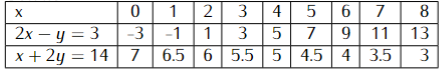
\includegraphics{images/Cpt15_table2.png}

\begin{figure}[H]

{\centering 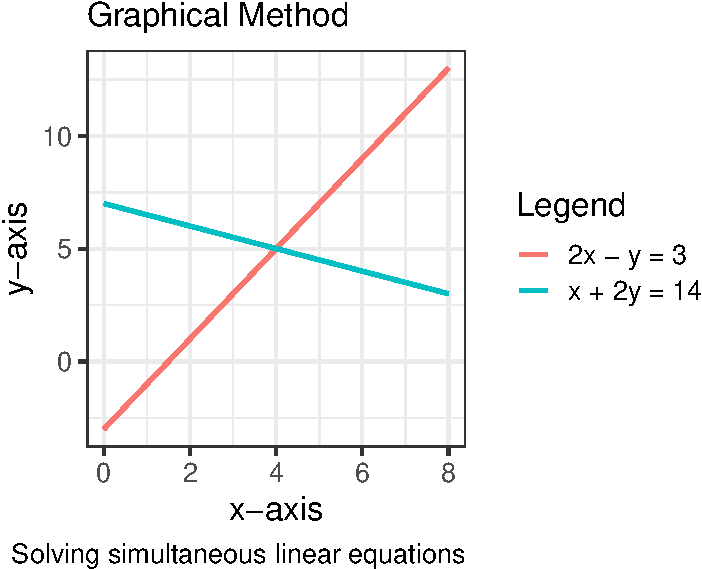
\includegraphics{Co-Ordinates-and-Graphs_files/figure-pdf/unnamed-chunk-2-1.pdf}

}

\caption{Solving simultaneous linear equations using graphical methods}

\end{figure}%

The solution of the two simultaneous equations is at the point of
interception as displayed in the figure above: From the graph, the
values of x and y are: \(x=4\) and \(y=5\)

\end{tcolorbox}

\begin{tcolorbox}[enhanced jigsaw, left=2mm, colframe=quarto-callout-note-color-frame, toptitle=1mm, opacitybacktitle=0.6, rightrule=.15mm, colbacktitle=quarto-callout-note-color!10!white, colback=white, arc=.35mm, breakable, leftrule=.75mm, bottomtitle=1mm, bottomrule=.15mm, title=\textcolor{quarto-callout-note-color}{\faInfo}\hspace{0.5em}{Problems to solve}, titlerule=0mm, coltitle=black, toprule=.15mm, opacityback=0]

\begin{enumerate}
\def\labelenumi{\arabic{enumi}.}
\tightlist
\item
  a) Use a graphical method to solve the following simultaneous
  equations: \hspace{2.5cm}(7mks)
\end{enumerate}

\begin{equation}
\begin{split}
3x-y&=4 \\
x+4y&=10
\end{split}
\end{equation}

\begin{verbatim}
 b) If the lines cut the y-axis at points P and Q respectively,
Write down the co-ordinates of the points P and Q.
\hspace{11cm}(3mks)
\end{verbatim}

\begin{enumerate}
\def\labelenumi{\arabic{enumi}.}
\setcounter{enumi}{1}
\item
  Copy and complete the tables below for:

  a) The linear equations \(3y=8+2x\) and \(y=5x-6\) respectively.
  \hspace{3.2cm}(4mks)

  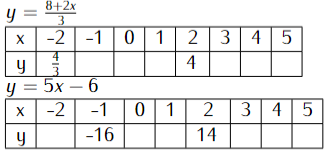
\includegraphics{images/Cpt15_Q2.png}

  b) On a graph paper and on the same grid draw the two linear equations
  in (a) above. \hspace{3.2cm} (4mks)

  c) What is the nature of the two graphs you have drawn?
  \hspace{4.6cm}(1mk)

  c) Use your graphs to solve the simultaneous equations.
  \hspace{4.8 cm}(1mk)

  \begin{equation}
  \begin{split}
  -2x+3y&=8 \\
  5x-y&=6
  \end{split}
  \end{equation}
\end{enumerate}

\end{tcolorbox}

\bookmarksetup{startatroot}

\chapter{Chapter Sixteen: Angles and Plane
Figures}\label{chapter-sixteen-angles-and-plane-figures}

\bookmarksetup{startatroot}

\chapter*{Angles and Plane Figures}\label{angles-and-plane-figures}
\addcontentsline{toc}{chapter}{Angles and Plane Figures}

\markboth{Angles and Plane Figures}{Angles and Plane Figures}

A plane is a flat surface, such as the walls of a classroom. Two planes
always intersect in a straight line. A vertex is a point where two lines
meet to form an angle.

\textbf{Types of angles}

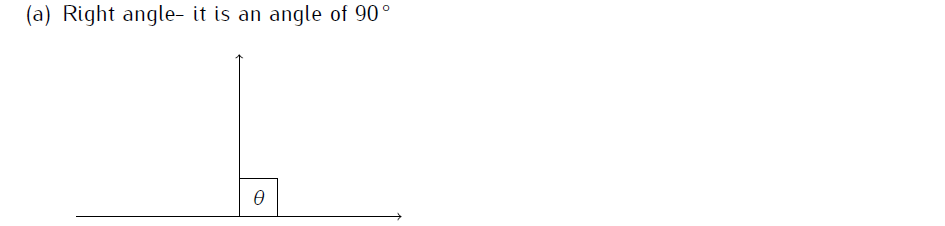
\includegraphics{images/Cpt15_anglesa.png}
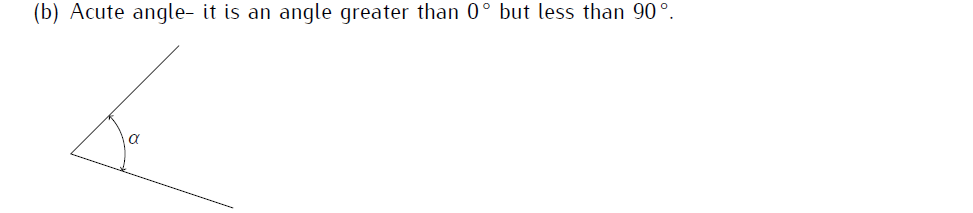
\includegraphics{images/Cpt15_anglesb.png}

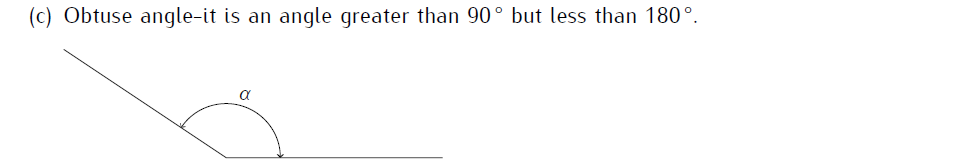
\includegraphics{images/Cpt15_anglesc.png}

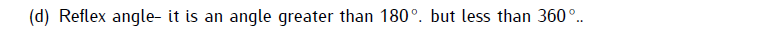
\includegraphics{images/Cpt15_anglesd.png}
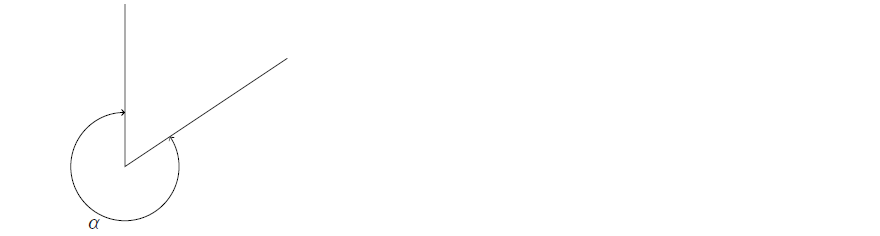
\includegraphics{images/Cpt15_anglesd2.png}
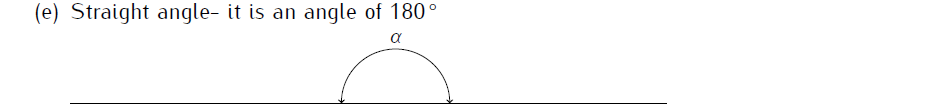
\includegraphics{images/Cpt15_anglese.png}
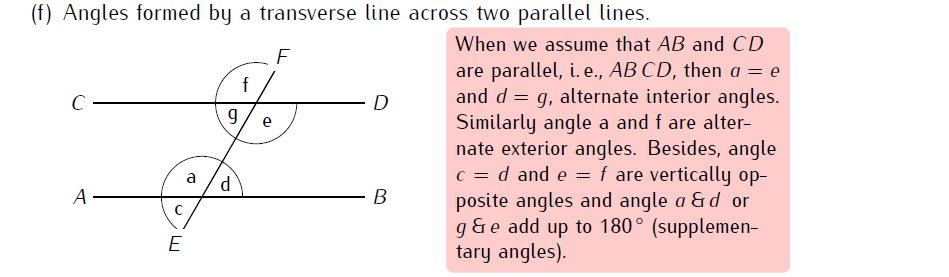
\includegraphics{images/Cpt15_anglesf.png}

\includegraphics{images/Cpt15_anglesg.png}

\textbf{Properties of angles}

i) Angles on a straight line add up to \(180\,^{\circ}\)

ii) Angles at a point add up to \(360\,^{\circ}\)

iii) Sum of interior angles of a regular polygon is given by:
\[Total \, interior \, angles
   =180^0(n-2)\] where \(n\) is the number of sides of the polygon

\[\therefore Each \,interior\, angle=\frac{180^0(n-2)}{n}\]

iv) Sum of exterior angles of a regular polygon is equal to \(360^0\)

\[\therefore Each\, exterior\, angle\,=\frac{360}{n}\]

v) Sum of an interior angle and an exterior angle is equal to \(180^0\)

\section{Solved Examples}\label{solved-examples-13}

\begin{tcolorbox}[enhanced jigsaw, left=2mm, colframe=quarto-callout-note-color-frame, toptitle=1mm, opacitybacktitle=0.6, rightrule=.15mm, colbacktitle=quarto-callout-note-color!10!white, colback=white, arc=.35mm, breakable, leftrule=.75mm, bottomtitle=1mm, bottomrule=.15mm, title=\textcolor{quarto-callout-note-color}{\faInfo}\hspace{0.5em}{Example 1}, titlerule=0mm, coltitle=black, toprule=.15mm, opacityback=0]

The sum of interior angles of two regular polygons of sides; n and
\(n + 2\) are in the ratio \(5:7\) Calculate the sum of the interior
angles of the polygon with n sides. \hspace{0.5cm} \((4 mks)\)

\end{tcolorbox}

\begin{tcolorbox}[enhanced jigsaw, left=2mm, colframe=quarto-callout-caution-color-frame, toptitle=1mm, opacitybacktitle=0.6, rightrule=.15mm, colbacktitle=quarto-callout-caution-color!10!white, colback=white, arc=.35mm, breakable, leftrule=.75mm, bottomtitle=1mm, bottomrule=.15mm, title=\textcolor{quarto-callout-caution-color}{\faFire}\hspace{0.5em}{Solution}, titlerule=0mm, coltitle=black, toprule=.15mm, opacityback=0]

\begin{align}
1^{st}\,Polygon&=180^0(n-2)\\
2^{nd}\, Polygon&=180^0(n+2-2)\\ \frac{\cancel{180^0}(n-2)}{\cancel{180^0}n}&=\frac{5}{7}\\7n-14&=5n
\end{align}

\begin{align}
\frac{\cancel{2}n}{\cancel{2}}&=\frac{\cancelto{7}{14}}{\cancel2}\\&=7\,sides\\
\therefore n\, sided \,polygon&=180^0(5)\\&=900^0
\end{align}

\end{tcolorbox}

\begin{tcolorbox}[enhanced jigsaw, left=2mm, colframe=quarto-callout-note-color-frame, toptitle=1mm, opacitybacktitle=0.6, rightrule=.15mm, colbacktitle=quarto-callout-note-color!10!white, colback=white, arc=.35mm, breakable, leftrule=.75mm, bottomtitle=1mm, bottomrule=.15mm, title=\textcolor{quarto-callout-note-color}{\faInfo}\hspace{0.5em}{Example 2}, titlerule=0mm, coltitle=black, toprule=.15mm, opacityback=0]

The exterior angle of a regular polygon is equal to two-thirds of the
interior angle. Calculate the number of sides of the polygon and give
its name. \((4mks)\)

\end{tcolorbox}

\begin{tcolorbox}[enhanced jigsaw, left=2mm, colframe=quarto-callout-caution-color-frame, toptitle=1mm, opacitybacktitle=0.6, rightrule=.15mm, colbacktitle=quarto-callout-caution-color!10!white, colback=white, arc=.35mm, breakable, leftrule=.75mm, bottomtitle=1mm, bottomrule=.15mm, title=\textcolor{quarto-callout-caution-color}{\faFire}\hspace{0.5em}{Solution}, titlerule=0mm, coltitle=black, toprule=.15mm, opacityback=0]

\begin{align}
Sum\,Exterior\,angles&=360^0\\Sum \,interior\,angles&=180^0(n-2)\\
Exterior\,angle+Interior\,angle&=180^0\\If\, interior\, angle&=x^0,\\Exterior \,angle&=\frac{2}{3}x
\end{align}

\begin{align}
x+\frac{2}{3}x&=180^0\\\frac{\cancel3}{\cancel5}\times \frac{\cancel5}{\cancel3}x&=\cancelto{36}{180^0}\times\frac{3}{\cancel5}\\&=36\times3\\\therefore interior\,angle\,&=108^0\\Exterior\, angle&=180^0-108^0\\\frac{360}{n}&=72\\n&=5;\, Pentagon
\end{align}

\end{tcolorbox}

\begin{tcolorbox}[enhanced jigsaw, left=2mm, colframe=quarto-callout-note-color-frame, toptitle=1mm, opacitybacktitle=0.6, rightrule=.15mm, colbacktitle=quarto-callout-note-color!10!white, colback=white, arc=.35mm, breakable, leftrule=.75mm, bottomtitle=1mm, bottomrule=.15mm, title=\textcolor{quarto-callout-note-color}{\faInfo}\hspace{0.5em}{Example 3}, titlerule=0mm, coltitle=black, toprule=.15mm, opacityback=0]

The sum of the interior angles of an n-sided polygon is \(1260^0\). Find
the value of n and hence deduce the name of the polygon. \((3mks)\)

\end{tcolorbox}

\begin{tcolorbox}[enhanced jigsaw, left=2mm, colframe=quarto-callout-caution-color-frame, toptitle=1mm, opacitybacktitle=0.6, rightrule=.15mm, colbacktitle=quarto-callout-caution-color!10!white, colback=white, arc=.35mm, breakable, leftrule=.75mm, bottomtitle=1mm, bottomrule=.15mm, title=\textcolor{quarto-callout-caution-color}{\faFire}\hspace{0.5em}{Solution}, titlerule=0mm, coltitle=black, toprule=.15mm, opacityback=0]

\begin{align}
Sum\,interior\,angles&=180(n-2)\\180(n-2)&=1260^0\\n-2&=7\\n&=9;\,Nonagon
\end{align}

\end{tcolorbox}

\begin{tcolorbox}[enhanced jigsaw, left=2mm, colframe=quarto-callout-note-color-frame, toptitle=1mm, opacitybacktitle=0.6, rightrule=.15mm, colbacktitle=quarto-callout-note-color!10!white, colback=white, arc=.35mm, breakable, leftrule=.75mm, bottomtitle=1mm, bottomrule=.15mm, title=\textcolor{quarto-callout-note-color}{\faInfo}\hspace{0.5em}{Problems to solve}, titlerule=0mm, coltitle=black, toprule=.15mm, opacityback=0]

\begin{enumerate}
\def\labelenumi{\arabic{enumi}.}
\item
  The size of an interior angle of a regular polygon is \(x^2\) while
  its exterior angle is \(3x\). Find the number of sides of the polygon
  \((4mks)\)
\item
  One interior angle of a polygon is equal to \(60\,^{\circ}\) and each
  of the other interior angles is \(132\,^{\circ}\). Find the number of
  sides and name of the polygon. \((3mks)\)
\item
  The difference between the exterior and interior angle of a regular
  polygon is \(120\,^{\circ}\). Determine the number of sides of the
  polygon. \hspace{8.3cm} \((3mks)\)
\item
  A regular polygon has internal angle of \(120\,^{\circ}\) and side of
  length 18cm.

  a) Find the number of sides of the polygon. \hspace{6.5cm} \((2mks)\)

  b) Find the perimeter of the polygon. \hspace{7.5cm} \((2mks)\)
\item
  The sum of the interior angles of a regular polygon is
  \(1800\,^{\circ}\). Calculate

  a) The number of sides of the polygon \hspace{7.4cm} \((2mks)\)

  b) The sizes of the exterior and interior angles of the polygon.
  \hspace{3.3cm} \((2mks)\)
\item
  The interior angle of a regular polygon is \(30\,^{\circ}\) more than
  four times the exterior angle of the same polygon. Determine the
  number of sides of the polygon. \hspace{4cm} \((3mks)\)
\item
  The size of an exterior angle of a regular polygon is \(\frac{2}{3}\)
  times the size of its interior angle. Find the number of sides of this
  polygon. \hspace{8.2cm} \((3mks)\)
\item
  The sum of the interior angles of an n-sided polygon is \(1440^0\).
  Find the value of n and hence deduce the name of the polygon.
  \hspace{9cm} \((3mks)\)
\item
  The sum of the interior angles of an n-sided polygon is \(1080^0\).
  Find the value of n and hence give the name of the polygon.
  \hspace{10cm} \((3mks)\)
\item
  A nine-sided polygon has three of its angles equal to and the other
  angles are \((2\theta - 30)\), \((\theta- 28)\), \(3(\theta - 4)\),
  \(\theta -45\), \(3\theta-20\), and \((126 - \theta)\). Calculate the
  value of \(\theta\). \hspace{4.2cm} \((3mks)\)
\item
  On a graph paper,

  a) Plot the points \(A(4, -1)\), \(B(5, -3)\), \(C(4, -4)\) and
  \(D(3, -3)\) and join the Points to form a polygon PQRS. State the
  name of the polygon formed. \hspace{4.5cm} \((2mks)\)

  b) Write down the equation of the line of symmetry of the polygon.
  \hspace{3.2cm}\((1mk)\)
\item
  In the figure below \(MNO =54\,^{\circ}\) and \(PLM =50\,^{\circ}\),
  \(PN = NM\) and PO is parallel to LM. Find the value of
  \(\sphericalangle LPM\)
\end{enumerate}

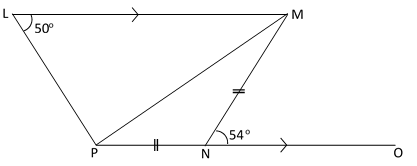
\includegraphics{images/trapezia.png}

\end{tcolorbox}

\bookmarksetup{startatroot}

\chapter{Chapter Seventeen: Geometrical
Constructions}\label{chapter-seventeen-geometrical-constructions}

\bookmarksetup{startatroot}

\chapter*{Geometrical Constructions}\label{geometrical-constructions}
\addcontentsline{toc}{chapter}{Geometrical Constructions}

\markboth{Geometrical Constructions}{Geometrical Constructions}

\textbf{Note:} To circumscribe a circle around a triangle, we bisect two
sides of the triangle and the point of intersection is the center of the
circle.

To inscribe a circle inside a triangle, we bisect two angles of the
triangle and the point of intersection is the center of the circle.

\textbf{Geometrical construction} is the drawing of accurate figures.
The figures are constructed using a pair of compasses and a ruler only

\textbf{Perpendicular Lines}

Figure 17.1 shows XY as a perpendicular bisector of a given line AB

\begin{figure}[H]

{\centering 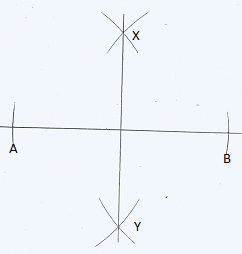
\includegraphics{figures/Images/FIG1.png}

}

\caption{Figure 17.1: Perpendicular Bisector}

\end{figure}%

Figure 17.2 shows PR, a perpendicular from point P to a given line AB.

\begin{figure}[H]

{\centering 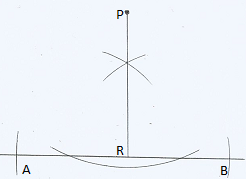
\includegraphics{figures/Images/FIG2.png}

}

\caption{Figure 17.2: Perpendicular Bisector from a Point}

\end{figure}%

\textbf{Constructing Angles of}
\(60\,^{\circ}, \,120\,^{\circ},\, and \,30\,^{\circ}\)

In this section, we will consider the construction of some angles with
special sizes using a pair of compasses and a ruler only.

\textbf{Constructing a} \(60^0\) \textbf{Angle}

\textbf{Step 1:} Draw the line AB.

\textbf{Step 2:} Place the tip of the compass at A and draw an arc of
any measure to cut the line AB at some point (say R).

\textbf{Step 3:} Keeping the width unchanged, place the tip of the
compass on point R and draw another arc cutting the arc drawn in the
previous step at some point (say S)

\textbf{Step 4:} Connect the points A and S with a straight line and
extend it to form a line AC.

The measure of the \(\angle BAC\) is \(60^0\)

\begin{figure}[H]

{\centering 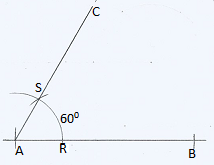
\includegraphics{figures/Images/FIG3.png}

}

\caption{Figure 17.3: An Angle of \(60^0\)}

\end{figure}%

\textbf{Constructing a} \(120^0\) \textbf{Angle}

\textbf{Step 1:} Draw the line AB. \textbf{\{Step 2:} Place the tip of
the compass at A and draw an arc of any measure to cut the line AB at
some point (say P). \textbf{Step 3:} Keeping the width unchanged, place
the tip of the compass on point P and draw another arc cutting the arc
drawn in the previous step at some point (say S) \textbf{Step 4:} With
the same width place the tip of the compass at point S and draw another
arc cutting the arc drawn in step 2 at some point (say T) \textbf{Step
5:} Connect the points A and T with a straight line and extend it to
form a line AC.

The measure of the \(\angle BAC\) is \(120^0\)

\begin{figure}[H]

{\centering 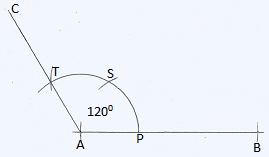
\includegraphics{figures/Images/FIG4.png}

}

\caption{Figure 17.4: An Angle of \(120^0\)}

\end{figure}%

\textbf{Constructing a} \(30^0\) \textbf{Angle}

To construct the angle of \(30^0\), Construct the angle of \(60^0\) as
described above and then bisect it as shown below.

The measure of the \(\angle BAC\) is \(30^0\)

\begin{figure}[H]

{\centering 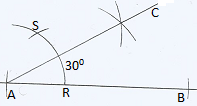
\includegraphics{figures/Images/FIG5.png}

}

\caption{Figure 17.5: An Angle of \(30^0\)}

\end{figure}%

\section{Solved Examples}\label{solved-examples-14}

\begin{tcolorbox}[enhanced jigsaw, left=2mm, colframe=quarto-callout-note-color-frame, toptitle=1mm, opacitybacktitle=0.6, rightrule=.15mm, colbacktitle=quarto-callout-note-color!10!white, colback=white, arc=.35mm, breakable, leftrule=.75mm, bottomtitle=1mm, bottomrule=.15mm, title=\textcolor{quarto-callout-note-color}{\faInfo}\hspace{0.5em}{Example 1}, titlerule=0mm, coltitle=black, toprule=.15mm, opacityback=0]

Using a ruler and pair of compasses only, construct triangle ABC in
which \(AB = 5cm, BC = 7cm\) and angle \(ABC =60 \,^{\circ}\). Drop a
perpendicular from A to meet BC at M. Measure AM and AC. \hspace{14.5cm}
(3mks)

\end{tcolorbox}

\begin{tcolorbox}[enhanced jigsaw, left=2mm, colframe=quarto-callout-caution-color-frame, toptitle=1mm, opacitybacktitle=0.6, rightrule=.15mm, colbacktitle=quarto-callout-caution-color!10!white, colback=white, arc=.35mm, breakable, leftrule=.75mm, bottomtitle=1mm, bottomrule=.15mm, title=\textcolor{quarto-callout-caution-color}{\faFire}\hspace{0.5em}{Solution}, titlerule=0mm, coltitle=black, toprule=.15mm, opacityback=0]

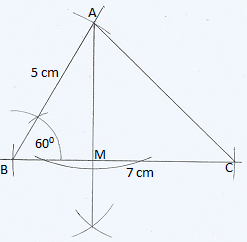
\includegraphics{figures/Images/triangle1.png}

\[AM=4.4\pm 0.1 \,cm\] \[AC=6.3\pm 0.1 \, cm\]

\end{tcolorbox}

\begin{tcolorbox}[enhanced jigsaw, left=2mm, colframe=quarto-callout-note-color-frame, toptitle=1mm, opacitybacktitle=0.6, rightrule=.15mm, colbacktitle=quarto-callout-note-color!10!white, colback=white, arc=.35mm, breakable, leftrule=.75mm, bottomtitle=1mm, bottomrule=.15mm, title=\textcolor{quarto-callout-note-color}{\faInfo}\hspace{0.5em}{Example 2}, titlerule=0mm, coltitle=black, toprule=.15mm, opacityback=0]

Use a ruler and a pair of compasses only for all constructions in this
question.

a) Construct a triangle ABC in which \(BC=9\, cm\), angle \(ABC=45^0\)
and angle \(ACB=75^0\) \hspace{14.2cm} (2mks)

b) Measure AB and AC. \hspace{10.6cm} (2mks)

c) At A drop a perpendicular to meet BC at D. \hspace{7cm} (1mk)

d) Measure AD and hence calculate the area of triangle
ABC.\hspace{4.4cm} (3mks)

e) Mark a point P on DA produced such that the area of triangle BPC is
half the area of triangle ABC. \hspace{13.3cm} (1mk)

f) Complete triangle BPC and measure PC \hspace{7.5cm} (1mk)

\end{tcolorbox}

\begin{tcolorbox}[enhanced jigsaw, left=2mm, colframe=quarto-callout-caution-color-frame, toptitle=1mm, opacitybacktitle=0.6, rightrule=.15mm, colbacktitle=quarto-callout-caution-color!10!white, colback=white, arc=.35mm, breakable, leftrule=.75mm, bottomtitle=1mm, bottomrule=.15mm, title=\textcolor{quarto-callout-caution-color}{\faFire}\hspace{0.5em}{Solution}, titlerule=0mm, coltitle=black, toprule=.15mm, opacityback=0]

a) 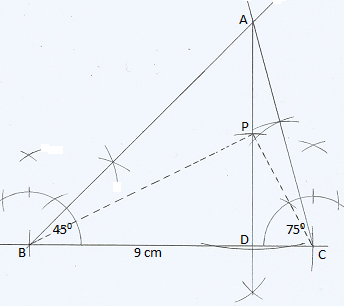
\includegraphics{figures/Images/Tria2.png}

b) \[AB=10\pm 0.1\, cm\]

\[AC=7.4\pm 0.1\,cm\]

d) \[AD=7.1\pm 0.1\,cm\] \textbf{Area of Triangle}
\(ABC=31.95\pm 0.45\, cm^2\)

c) \[PC=4.1\pm 0.1\,cm\]

\end{tcolorbox}

\begin{tcolorbox}[enhanced jigsaw, left=2mm, colframe=quarto-callout-note-color-frame, toptitle=1mm, opacitybacktitle=0.6, rightrule=.15mm, colbacktitle=quarto-callout-note-color!10!white, colback=white, arc=.35mm, breakable, leftrule=.75mm, bottomtitle=1mm, bottomrule=.15mm, title=\textcolor{quarto-callout-note-color}{\faInfo}\hspace{0.5em}{Example 3}, titlerule=0mm, coltitle=black, toprule=.15mm, opacityback=0]

Use a ruler and a pair of compasses only for all constructions in this
question.

a) Construct triangle PQR in which QR=8.5cm, PQ=7cm and angle
PQR\(=60^0\) \hspace{1.2cm} (3 mks)

b) Measure PR and angle QPR. \hspace{9cm} (2 mks)

c) Construct a circle which is inscribed inside triangle
PQR.\hspace{4.7cm}(4mks)

d) Measure the radius of this circle. \hspace{8.4cm} (1 mk)

\end{tcolorbox}

\begin{tcolorbox}[enhanced jigsaw, left=2mm, colframe=quarto-callout-caution-color-frame, toptitle=1mm, opacitybacktitle=0.6, rightrule=.15mm, colbacktitle=quarto-callout-caution-color!10!white, colback=white, arc=.35mm, breakable, leftrule=.75mm, bottomtitle=1mm, bottomrule=.15mm, title=\textcolor{quarto-callout-caution-color}{\faFire}\hspace{0.5em}{Solution}, titlerule=0mm, coltitle=black, toprule=.15mm, opacityback=0]

a) \includegraphics{figures/Images/Tria3.png}

b) \[PR=7.8\pm 0.1\, cm\] \[\angle QPR=70 \pm 1^0\]

c) Radius\(=2.2\pm 0.1\,cm\)

\end{tcolorbox}

\begin{tcolorbox}[enhanced jigsaw, left=2mm, colframe=quarto-callout-note-color-frame, toptitle=1mm, opacitybacktitle=0.6, rightrule=.15mm, colbacktitle=quarto-callout-note-color!10!white, colback=white, arc=.35mm, breakable, leftrule=.75mm, bottomtitle=1mm, bottomrule=.15mm, title=\textcolor{quarto-callout-note-color}{\faInfo}\hspace{0.5em}{Problems to solve}, titlerule=0mm, coltitle=black, toprule=.15mm, opacityback=0]

\begin{enumerate}
\def\labelenumi{\arabic{enumi}.}
\item
  a) Using a pair of compasses and a ruler only construct a triangle ABC
  such that \$AB= 6.5cm, BC = 5cm \$ and angle \(ABC = 135\,^{\circ}\)
  \hspace{5cm} (2mks)

  b) Construct the height of triangle ABC in (a) above taking AB as the
  base, hence calculating the area of triangle ABC. \hspace{8.9cm}
  (2mks)
\item
  Using compass and ruler only construct a triangle ABC such that AB
  7cm, BC = 6cm and angle \(ABC = 67.5\,^{\circ}\) measure the length of
  AC. \hspace{6.1cm} ( 4mks)
\item
  Use a ruler and a pair of compasses only for all the constructions in
  this question.

  a) Construct a triangle PQR in which PQ=9 cm, QR=6 cm and angle
  PQR\(=30^0\) \hspace{0.2cm} (3mks)

  b) From P drop a perpendicular to meet QR produced at S.\hspace{4cm}
  (1mk)

  c) Measure PS and hence calculate the area of triangle
  PQR.\hspace{3.4cm} (2mks)

  d) Locate a point T on SP produced such that the area of triangle QTR
  is \(\frac{4}{3}\) times the area of triangle PQR. \hspace{10.8cm}
  (2mks)

  e) Complete triangle QTR and measure RT and angle TQR.\hspace{3.9cm}
  (2mks)
\item
  Use a ruler and a pair of compasses only for all constructions in this
  question.

  a) Construct triangle ABC in which BC=AC=7 cm and angle ACB\(=37.5^0\)
  \hspace{1.4cm}(3mks) b) Measure AB. \hspace{10.9cm} (1mk)

  c) From A drop a perpendicular to meet BC produced at D.\hspace{4cm}
  (1mk)

  d) Measure AD and hence calculate the area of triangle
  ABC.\hspace{3.4cm} (2mks)

  e) Mark a point P on AD such that the area of triangle PBC is half the
  area of triangle ABC. \hspace{12.2cm} (1mk)

  f) Complete triangle PBC and measure angle PBC \hspace{5.1cm} (2mks)
\item
  Use a ruler and a pair of compasses only for all constructions in this
  question.

  a) Construct triangle PQR in which QR=5cm, PR=7 cm and PRQ\(=150^0\)
  \hspace{1.4cm}(3mks) b) Measure PQ and angle PQR. \hspace{8cm} (2mks)

  c) From P drop a perpendicular to meet QR produced at D.\hspace{3.8cm}
  (1mk)

  d) Mark a point T on DP produced such that the area of triangle TQR is
  twice the area of triangle PQR \hspace{10.8cm} (2mks)

  e) Complete triangle TQR and measure angle QRT. \hspace{5cm} (2mks)
\item
  Use a ruler and a pair of compasses only for all constructions in this
  question

  a) Construct triangle ABC in which BC=7 cm, and angle ABC\(=45^0\) and
  angle ACB\(=60^0\). \hspace{13.25cm}(3mks)

  b) Measure AB and AC \hspace{9.6cm} (2mks)

  c) Construct a circle that touches BC at B and passes through
  A.\hspace{3cm}(4mks)

  d) Measure the radius of the circle \hspace{7.8cm} (1mk)
\item
  Use a ruler and a pair of compasses only for all constructions in this
  question.

  a) Construct triangle ABC in which BC=7cm, angle ABC=22.50 and angle
  ACB\(=120^0\). \hspace{12.9cm} (4mks)

  b) Measure AC \hspace{10.8cm} (1mk)

  c) Produce AB to D and AC to E and bisect angle CBD and angle
  BCE.\hspace{1.4cm} (2mks)

  d) Construct a circle which touches all three sides AD, BC, and
  AE.\hspace{1.7cm}(2mks)

  e) What is the radius of this circle? \hspace{7.4cm} (1mk)
\end{enumerate}

\end{tcolorbox}

\bookmarksetup{startatroot}

\chapter{Chapter Eighteen: Scale
Drawing}\label{chapter-eighteen-scale-drawing}

\bookmarksetup{startatroot}

\chapter*{Scale Drawing}\label{scale-drawing}
\addcontentsline{toc}{chapter}{Scale Drawing}

\markboth{Scale Drawing}{Scale Drawing}

\section{Bearing and Distance, Angles of Elevation and
Depression}\label{bearing-and-distance-angles-of-elevation-and-depression}

\textbf{Types of bearing}

\begin{itemize}
\item
  \textbf{True Bearing}- It can only measured from North pole in a
  clockwise direction and given in three digits format. For example
  given that \(065^0\) is the bearing between two points, say \(A\) from
  \(B\); the angle is obtained at point \(B\) from north pole in a
  clockwise direction to the line joining \(A\).
\item
  \textbf{Compass bearing}- It can be measured from either North or
  South pole in either clockwise or anticlockwise direction depending on
  the side the target object is located. For example if point \(A\) is
  \(60^0\) North-West of point \(B\), then point \(A\) is on a compass
  bearing of \(N60^0W\) from point \(B\).
\end{itemize}

\section{Solved Examples}\label{solved-examples-15}

\begin{tcolorbox}[enhanced jigsaw, left=2mm, colframe=quarto-callout-note-color-frame, toptitle=1mm, opacitybacktitle=0.6, rightrule=.15mm, colbacktitle=quarto-callout-note-color!10!white, colback=white, arc=.35mm, breakable, leftrule=.75mm, bottomtitle=1mm, bottomrule=.15mm, title=\textcolor{quarto-callout-note-color}{\faInfo}\hspace{0.5em}{Example 1}, titlerule=0mm, coltitle=black, toprule=.15mm, opacityback=0]

Three towns A, B, and C are situated such that town B is 40km on a
bearing of 0400 from town A. Town C is 100 km on a bearing of 1300 from
town B.

\begin{enumerate}
\def\labelenumi{(\alph{enumi})}
\item
  Draw a sketch showing the positions of towns A, B, and C. \((1mk)\)
\item
  Calculate:

  i. The size of angle ABC \((1mk)\)

  ii. The distance of C from A to 1 decimal place \((2mk)\)
\end{enumerate}

\end{tcolorbox}

\begin{tcolorbox}[enhanced jigsaw, left=2mm, colframe=quarto-callout-caution-color-frame, toptitle=1mm, opacitybacktitle=0.6, rightrule=.15mm, colbacktitle=quarto-callout-caution-color!10!white, colback=white, arc=.35mm, breakable, leftrule=.75mm, bottomtitle=1mm, bottomrule=.15mm, title=\textcolor{quarto-callout-caution-color}{\faFire}\hspace{0.5em}{Solution}, titlerule=0mm, coltitle=black, toprule=.15mm, opacityback=0]

\begin{enumerate}
\def\labelenumi{(\alph{enumi})}
\tightlist
\item
\end{enumerate}

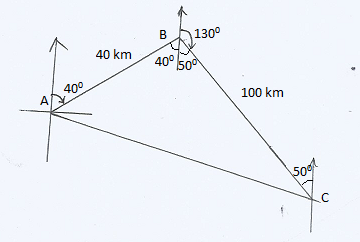
\includegraphics{figures/exa1.png}

\begin{enumerate}
\def\labelenumi{(\alph{enumi})}
\setcounter{enumi}{1}
\item
  i. \(\angle ABC ??? 40^0 + 50^0 = 90^0\)

  ii. \[AC^2 = AB^2 + BC^2\] \[AC^2 = 40^2 + 100^2\] \[AC^2 = 11,600\]
  \[AC = 107.7\,Km\]
\end{enumerate}

\end{tcolorbox}

\begin{tcolorbox}[enhanced jigsaw, left=2mm, colframe=quarto-callout-note-color-frame, toptitle=1mm, opacitybacktitle=0.6, rightrule=.15mm, colbacktitle=quarto-callout-note-color!10!white, colback=white, arc=.35mm, breakable, leftrule=.75mm, bottomtitle=1mm, bottomrule=.15mm, title=\textcolor{quarto-callout-note-color}{\faInfo}\hspace{0.5em}{Example 2}, titlerule=0mm, coltitle=black, toprule=.15mm, opacityback=0]

A dove flies from a tree A to another tree B which is \(80\, m\) on a
bearing of \(060^0\) from A. From B the dove flies \(100\, m\) to tree C
which is on a compass bearing of \(S40^0E\) from tree B and finally
flies due south to another tree D which is on a bearing of \(1^0\) from
A. a) Using a ruler and a pair of compasses only construct an accurate
scale drawing showing the positions of A, B, C, and D.
\((scale : 1\, cm=10\, m)\)

b) By measurement from your scale drawing determine:

(i) The distance and compass bearing of A from C. \((2mks)\)

(ii) The distance of D from C. \((1mks)\)

(iii) The distance and compass bearing of A from D \((2mks)\)

\end{tcolorbox}

\begin{tcolorbox}[enhanced jigsaw, left=2mm, colframe=quarto-callout-caution-color-frame, toptitle=1mm, opacitybacktitle=0.6, rightrule=.15mm, colbacktitle=quarto-callout-caution-color!10!white, colback=white, arc=.35mm, breakable, leftrule=.75mm, bottomtitle=1mm, bottomrule=.15mm, title=\textcolor{quarto-callout-caution-color}{\faFire}\hspace{0.5em}{Solution}, titlerule=0mm, coltitle=black, toprule=.15mm, opacityback=0]

(a)

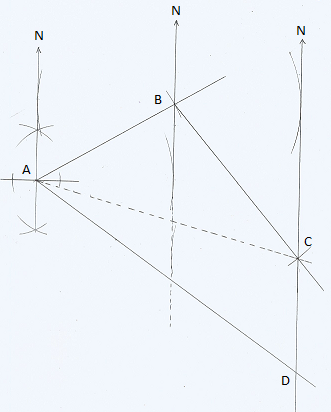
\includegraphics{figures/exa2.png}

(b)

(i) Distance of A from \(C = 139 ? 1 m\) ;

Compass bearing of A from \(C = N 75^0 ? 10 W\)

(ii) Distance of D from \(C = 58 ? 1m\)

(iii) Distance of A from \(D = 164 ? 1m\) ;

Compass bearing of A from \(D = N 55^0 ? 10 W\)

\end{tcolorbox}

\begin{tcolorbox}[enhanced jigsaw, left=2mm, colframe=quarto-callout-note-color-frame, toptitle=1mm, opacitybacktitle=0.6, rightrule=.15mm, colbacktitle=quarto-callout-note-color!10!white, colback=white, arc=.35mm, breakable, leftrule=.75mm, bottomtitle=1mm, bottomrule=.15mm, title=\textcolor{quarto-callout-note-color}{\faInfo}\hspace{0.5em}{Example 3}, titlerule=0mm, coltitle=black, toprule=.15mm, opacityback=0]

The angle of elevation of the top of a vertical tower from a point P is
\(35^0\). The angle of elevation of the top of the tower from another
point Q which is nearer the foot R of the tower is \(50^0\). The
distance between Q and P is \(40\, m\) and the points P, Q, and R are on
the same straight line on level ground.

(a) Use a scale of 1cm to represent 10 m, draw an accurate scale drawing
to represent the above information. \((4mks)\)

(b) Use your scale drawing to determine:

(i) The height of the tower \((2mks)\)

(ii) The distance QP \((2mks)\)

(iii) The distance of P from the top of the tower \((2mks)\)

\end{tcolorbox}

\begin{tcolorbox}[enhanced jigsaw, left=2mm, colframe=quarto-callout-caution-color-frame, toptitle=1mm, opacitybacktitle=0.6, rightrule=.15mm, colbacktitle=quarto-callout-caution-color!10!white, colback=white, arc=.35mm, breakable, leftrule=.75mm, bottomtitle=1mm, bottomrule=.15mm, title=\textcolor{quarto-callout-caution-color}{\faFire}\hspace{0.5em}{Solution}, titlerule=0mm, coltitle=black, toprule=.15mm, opacityback=0]

(a)

\includegraphics{figures/Tria3.png}

(b)

(i) Height of the tower \(= 68 \pm 1m\)

(ii) \(RQ = 58 \pm 1 m\)

(iii) Distance of P from top of the tower \(= 120 \pm 1 m\)

\end{tcolorbox}

\begin{tcolorbox}[enhanced jigsaw, left=2mm, colframe=quarto-callout-note-color-frame, toptitle=1mm, opacitybacktitle=0.6, rightrule=.15mm, colbacktitle=quarto-callout-note-color!10!white, colback=white, arc=.35mm, breakable, leftrule=.75mm, bottomtitle=1mm, bottomrule=.15mm, title=\textcolor{quarto-callout-note-color}{\faInfo}\hspace{0.5em}{Example 4}, titlerule=0mm, coltitle=black, toprule=.15mm, opacityback=0]

The following measurement were recorded in a book of a virgin land using
PQ as the base line. And \(PQ=400 \,m\)

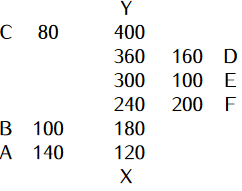
\includegraphics{Images/CH18_E4.png}

a) Using a scale of 1: 4000, draw an accurate map of the farm.
\((4mks)\)

b) Determine the actual area of the farm in hectares.\((4mks)\)

c) If the farm is on sale at 320,000 per hectare, Find how much the farm
costs.\((2mks)\)

\end{tcolorbox}

\begin{tcolorbox}[enhanced jigsaw, left=2mm, colframe=quarto-callout-caution-color-frame, toptitle=1mm, opacitybacktitle=0.6, rightrule=.15mm, colbacktitle=quarto-callout-caution-color!10!white, colback=white, arc=.35mm, breakable, leftrule=.75mm, bottomtitle=1mm, bottomrule=.15mm, title=\textcolor{quarto-callout-caution-color}{\faFire}\hspace{0.5em}{Solution}, titlerule=0mm, coltitle=black, toprule=.15mm, opacityback=0]

a)

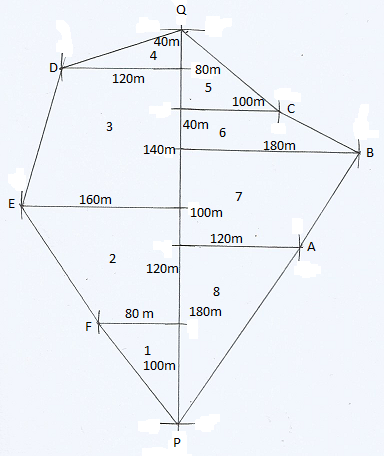
\includegraphics{figures/survey.png} b) The Area of the farm is given as
follows:

\begin{align*}
Label \,1 &\Rightarrow &\frac{1}{\cancel2}\times \cancelto{50}{100}\times80&=4,000 \,m^2\\
Label\,2 &\Rightarrow &\frac{1}{\cancel2}\times \cancelto{60}{120}\times(160+80)&=14,400\,m^2\\
Label\,3 &\Rightarrow &\frac{1}{\cancel2}\times \cancelto{70}{140} \times (120+160)&=19,600 \,m^2\\
Label\,4 &\Rightarrow &\frac{1}{\cancel2} \times \cancelto{20}{40}\times 120&=2,400 \,m^2\\
Label \,5 &\Rightarrow &\frac{1}{\cancel2}\times \cancelto{40}{80}\times100&=4,000 \,m^2\\
Label \, 6 &\Rightarrow &\frac{1}{\cancel2}\times \cancelto{20}{40}\times (100+180)&=5,600\,m^2\\
Label \, 7 &\Rightarrow &\frac{1}{\cancel2}\times \cancelto{50}{100}\times(180+120)&=15,000\,m^2\\
Label \,8 &\Rightarrow &\frac{1}{\cancel2}\times \cancel{90}{180}\times120&=10,800\, m^2\\
\end{align*}

\[\therefore The\,total\, Area \, of\, the \,Farm \Rightarrow \frac{75,8\cancel{00}}{10,0\cancel{00}}=7.58 \,ha
\]

c) The farm cost is given by:

\[\Rightarrow 7.58\times320,000=Ksh. 2,425,600\]

\end{tcolorbox}

\begin{tcolorbox}[enhanced jigsaw, left=2mm, colframe=quarto-callout-note-color-frame, toptitle=1mm, opacitybacktitle=0.6, rightrule=.15mm, colbacktitle=quarto-callout-note-color!10!white, colback=white, arc=.35mm, breakable, leftrule=.75mm, bottomtitle=1mm, bottomrule=.15mm, title=\textcolor{quarto-callout-note-color}{\faInfo}\hspace{0.5em}{Problems to solve}, titlerule=0mm, coltitle=black, toprule=.15mm, opacityback=0]

\begin{verbatim}
1.  The scale of a map is given as $1:50,000$. Find the actual area
    in hectares of a region represented by a right-angled triangle
    of base 5cm and height 6cm. $(3mks)$

2.  The angle of elevation of the top of a flag post from point A on
    a level ground is $24\,^{\circ}$. The angle of elevation of the
    top of the flag post from another point B nearer the flag post
    and 20m from A is $36\,^{\circ}$.

    a\) Use a scale of 1cm to represent 5 m, and draw an accurate
    scale drawing to represent the above information.
    $(4mks)$

    b\) The height of the flag post. $(2mks)$

    c\) The distance from point B to the top of the flagpole.
    $(2mks)$

    d\) Distance of A from the top of the flag post.
    $(2mks)$

3.  A plane leaves town P to town Q on a bearing of \$
    120,\^{\circ}\$and a distance of 300km. It then flies 400km on a
    bearing of $050\,^{\circ}$ to town R. Find, by scale drawing the
    distance and compass bearing of P from R.
    $(3mks)$

4.  Three ports A, B, and C are situated in such a way that port A
    is 140km on a compass bearing of $N\,60^0\, E$ from port B. Port
    C is 180km on a compass bearing of $S\,30^0\, E$ from A. A ship
    S is docked in the sea, 90km on a bearing of $190^0$ from port

    B.  

    a\) Using a scale of 1cm to represent 20km, draw a diagram to
    show the position of ports A, B, C, and ship S.
    $(4mks)$

    b\) Using your diagram find

    i\) The distance between the ship and the port A
    $(1mk)$

    ii\) The distance and bearing of the ship from port C
    $(2mks)$

    iii\) The distance from B to C $(1mk)$

    iv\) Compass bearing of S from A $(2mks)$

5.  Four schools Mucagara, Kerugoya, Kiamutugu, and Kiburia are such
    that Kerugoya is 22 km from Mucagara on a bearing of
    $220\,^{\circ}$, Kiamutugu is to the east of Mucagara and 6 km
    away while Kiburia is 8 km on a compass bearing of $S42^0E$ from
    Kiamutugu.

    a\) Using a scale of 1:200,000 draw a scale diagram showing the
    relative positions of the four schools. $(5mks)$

    b\) Using your diagram determine the distance and bearing of
    Kiburia from Kerugoya $(2mks)$

    c\) The distance and compass bearing of Kerugoya from Kiamutugu
    $(3mks).$

6.  Four towns P, R, T, and S are such that R is 90km directly to
    the north of P and T is on a Bearing of $295\,^{\circ}$ from P
    at a distance of 75km. S is on a compass bearing
    $N30\,^{\circ}W$ from T and a distance of 40km.

    a\) Using a scale of 1cm to represent 10km, make an accurate
    scale drawing to show the relative position of the towns.
    $(4mks)$

    b\) Find:

    i\) The distance and the bearing of R from T
    $(2mks)$

    ii\) The distance and the bearing of S from R
    $(2mks)$

    iii\) The compass bearing of P from S $(2mks)$

7.  Two airplanes, T and S leave airport A at the same time. S flies
    on a bearing of $062\,^{\circ}$ at 600km/h while T flies on a
    bearing of $290\,^{\circ}$ at 750 km/h.

    a\) Use a suitable scale, to draw a diagram showing the relative
    position of the airplanes after two hours.
    $(3mks)$

    b\) Use your diagram to determine:

    i\) The distance between the two airplanes.
    $(2mks)$

    ii\) The bearing of T from S. $(1mk)$

    c\) Aeroplane T later flew to the East at the same speed for one
    hour. Show its final position on the diagram in (a) above.
    Determine:

    i\) Its final distance from A.$(2mks)$

    ii\) Its final bearing from S. $(1mk)$

8.  Three Kenyan warships A, B, and C are at sea such that ship B is
    520km on a bearing of $040^{\circ}$ from ship A. Ship C is 600km
    from ship B on a bearing of $130\,^{\circ}$. An enemy ship D is
    sighted 900km due south of ship B.

    a\) Taking a scale of 1cm to represent 100km locate the position
    of the ships A, B, C, and D. $(4mks)$

    b\) Find the compass bearing of:

    i\) Ship A from ship D $(1mk)$

    ii\) Ship D from ship C $(1mk)$

    c\) Use the scale drawing to determine

    i\) The distance of D from A $(1mk)$

    ii\) The distance of C from D $(1mk)$

    d\) Find the bearing of:

    i\) B from C $(1mk)$

    ii\) A from C $(1mk)$

9.  An expedition has 5 sections AB, BC, CD, DE, and EA. B is 250 m
    on a bearing of $060\,^{\circ}$ from A. C is 520 m from B. The
    bearing of B from C is $310\,^{\circ}$. D is 430m on a bearing
    $240\,^{\circ}$ from C. E is 220 m on a bearing $023\,^{\circ}$
    from D.

    a\) Sketch the route $(1mk)$

    b\) Use a scale of 1cm to 50m to draw an accurate diagram
    representing the route. $(5mks)$

    c\) Use your diagram to determine

    i\) The distance in metres and bearing of A from E
    $(2mks)$

    ii\) Compass bearing of D from A $(2mks)$

10. Three boats X, Y, and Z are approaching a harbour H. X is 60km
    from the harbour on a bearing of $80\,^{\circ}$. Y is 75 km from
    the harbour on a bearing of $135\,^{\circ}$ and Z is due West of
    Y and on a bearing of $210\,^{\circ}$ from the harbour.

    a\) Using a scale of 1cm rep 10km make a scale drawing showing
    the positions of the three boats relative to the harbour.
    $(4mks)$

    b\) i) Using the scale drawing find; the distance and bearing of
    Y and X. $(2mks)$

    ii) The distance of Z from the harbour. $(2mks)$

    iii) The distance and compass bearing of Z from X.
         $(3mks)$

11. An aircraft leaves point A and flies on a bearing of
    $030\,^{\circ}$ to a second point B, which is 500km from A. From
    B, the aircraft then flies on a bearing of $328\,^{\circ}$ to a
    third point C which is 800km from B. The aircraft then flies
    directly back to A from C at a speed of 200 km/h.

    a\) Using a scale of 1cm rep 100Km make a scale drawing showing
    the positions of the aircraft. $(4mks)$

    b\) Time taken to fly directly from C to A.
    $(2mks)$

    c\) The bearing in which it would fly from C to A.
    $(1mk)$

    d\) Locate point D on a bearing $210\,^{\circ}$ from C and on a
    compass bearing of $N45\,^{\circ}W$ from A. Calculate BD in
    kilometers. $(2mks)$

    e\) What is the bearing of D from B? $(1mk)$

12. Five towns V, W, X, UY, and Z are situated such that W is 250km
    east of V. X is 320km from W on a bearing of $145\,^{\circ}$. Y
    is 380km on a bearing of $225\,^{\circ}$ from X. Z is on a
    compass bearing of $40\,^{\circ}$ from V but $278\,^{\circ}$
    from X.

    a\) Draw the diagram representing the position of the towns.
    (Use a scale of 1cm to represent 50km). $(4mks)$

    b\) From the diagram determine

    i)  The distance in km of V from Z $(1mk)$

    ii) The Compass bearing of Y from W $(2mks)$

    c\) A plane heading to town X takes off from town Y and flies
    upwards of a constant angle which is less than $90\,^{\circ}$.
    After flying a distance of 390km in the air it sees town X at an
    angle of depression of $35\,^{\circ}$. Calculate the distance of
    the plane from X at this point. $(3mks)$

13. A bird flies from a tree P to another tree Q which is 95 metres
    on a bearing of $040\,^{\circ}$ from P. From Q the bird flies 55
    metres due East to another tree R and finally flies due South to
    another tree S which is on a compass bearing of $S35\,^{\circ}E$
    from Q.

    a\) Construct an accurate scale drawing showing the positions of
    P, Q, R, and S. Use a scale of
    $(1cm = 10m)$.  $(4mks)$

    b\) i) From your diagram measure the distance and compass
    bearing of P from R. $(3mks)$

    ii) The distance of S from R in metres. $(1mk)$

    iii) The distance and bearing of S from P in metres.
         $(2mk)$
\end{verbatim}

\end{tcolorbox}

\bookmarksetup{startatroot}

\chapter*{SECTION TWO}\label{section-two}
\addcontentsline{toc}{chapter}{SECTION TWO}

\markboth{SECTION TWO}{SECTION TWO}

\bookmarksetup{startatroot}

\chapter*{Model Samples Papers}\label{model-samples-papers}
\addcontentsline{toc}{chapter}{Model Samples Papers}

\markboth{Model Samples Papers}{Model Samples Papers}

\begin{tcolorbox}[enhanced jigsaw, left=2mm, colframe=quarto-callout-note-color-frame, toptitle=1mm, opacitybacktitle=0.6, rightrule=.15mm, colbacktitle=quarto-callout-note-color!10!white, colback=white, arc=.35mm, breakable, leftrule=.75mm, bottomtitle=1mm, bottomrule=.15mm, title=\textcolor{quarto-callout-note-color}{\faInfo}\hspace{0.5em}{Model Sample Paper 1}, titlerule=0mm, coltitle=black, toprule=.15mm, opacityback=0]

\ul{\textbf{SECTION A: (50 MARKS)}}

\textbf{Answer all the question in this section}

\begin{enumerate}
\def\labelenumi{\arabic{enumi}.}
\tightlist
\item
  Evaluate without using tables or calculators. \((3mks)\)
\end{enumerate}

\[ \frac{\frac{3}{7}\,of\,28\div80\times-\frac{40}{3}}{-2\times5+(14\div7)\times3}\]

\begin{enumerate}
\def\labelenumi{\arabic{enumi}.}
\setcounter{enumi}{1}
\item
  Felix has four times as many ducks as hens and three-quarters as many
  turkeys as ducks.

  a) If he has x hens, write down a simplified expression in x for the
  total number of birds \((2mks)\)

  b) Find the total number of birds given that the Felix has 45
  turkeys.\((2mks)\)
\item
  Given that \(x=4,\, y= -2,\, and \,z= -3\) evaluate. \((3mks)\)
\end{enumerate}

\[ \frac{2(x+z)^2-(x-y)(y-z)}{4(x+y)-2(y-z)}\]

\begin{enumerate}
\def\labelenumi{\arabic{enumi}.}
\setcounter{enumi}{3}
\item
  Using a ruler and a pair of compasses only, construct triangle PQR in
  which \(PQ = 5.2cm\) \(QR=7.5cm\) and Angle \(PQR = 45^0\). By
  construction bisect angle PQR to meet line PR at a point M. find the
  ratio \(PM:MR\).\((3mks)\)
\item
  Use square and square root table to evaluate to 4 significant figures,
  the expression. \((3mks)\)
\end{enumerate}

\[\sqrt[]{24.640-(4.362)^2} \]

\begin{enumerate}
\def\labelenumi{\arabic{enumi}.}
\setcounter{enumi}{5}
\item
  The cost of a TV outside is US\$ 1200. Kelvin decides to buy one TV
  through an agent who deals with Japanese Yen. The agent charges him a
  commission of 5\% on the price of the TV and further 2,000 Yen as
  important tax. To the nearest Ksh. how much will he need to send to
  the agent to obtain the TV, given that:- \((3mks)\)

  \(1\,US\, \$ = 110.95 \,Yen\)

  \(1\,US \$ = Kshs. \,102.80\)
\item
  A two --digit number is such that the sum of the ones digit and the
  tens digit is 4. If the digits are reversed, the number formed exceeds
  the original number by 18. Find the number. \((3mks)\)
\item
  Metal block of side 5.6 cm was melted and the molten material used to
  make a sphere. In three significant figures, find the radius of the
  sphere in metres (take \(\pi =\frac{22}{7}\)) \((3mks)\)
\item
  Solve the simultaneous equations \((3mks)\)
\end{enumerate}

    \begin{align*}
     x+3y&=9\\
     4x-8y&=-4
    \end{align*}

\begin{enumerate}
\def\labelenumi{\arabic{enumi}.}
\setcounter{enumi}{9}
\item
  Kinyua bought soya and millet at Ksh. 70 per kg and Ksh. 40 per kg
  respectively. He then mixed them and sold the mixture at Ksh. 60 per
  kg making a profit of 20\%. Determine the ratio of soya to millet in
  mixture. \((3mks)\)
\item
  An aircraft left Nairobi at 2245h on Monday and arrived in Cape Town
  on Tuesday at 0300h. It departed from Cape Town at 0330h and arrived
  in Washington DC at 0630h on Wednesday. Find the travel ling time for
  the whole journey from Nairobi to Washington DC took? \((3mks)\)
\item
  A town B is 250 km due east of town A. Another town C is 200 km on a
  compass bearing of \(S40^0E\) from town B. use scale drawing to find
  the distance and bearing of town C from A. \((4mks)\)
\item
  1.784 kg of sugar whose density is \(1.08g/cm^3\) and 0.744kg of salt
  whose density is \(1.04g/cm^3\) are mixed together for a certain
  experiment. What is the density of the mixture in \(kg/m^3\)? ( Give
  the answer to 4. s.f) \((3mks)\)
\item
  The interior angle of a regular polygon is 5 times the exterior angle.
  How many sides does the polygon have? \((2mks)\)
\item
  Find the least number of steps in staircase if, when I go up 3 steps
  at a time, 4 steps at a time or 6 steps at a time, there is always 1
  step remaining at the top. \((3mks)\)
\item
  An arc of a circle of length 37.4cm subtends an angle of \(153^0\) at
  the centre of the circle. Calculate the area of the sector bounded by
  this arc. Take \(\pi=\frac{22}{7}\). \((4mks)\)
\end{enumerate}

\ul{\textbf{SECTION B (50 MARKS)}}

\textbf{\emph{Attempt all the questions}}

\begin{enumerate}
\def\labelenumi{\arabic{enumi}.}
\setcounter{enumi}{16}
\item
  Kirote and Kanze bought a bus which could carry 50 passengers when
  full. The bus uses Nairobi-Machakos route and charges Ksh. 160 per
  passengers for one way. The bus makes three trips between the two
  towns daily. The cost of fuel was Ksh. 2500 per day. The driver and
  the conductor are paid allowances of Ksh. 1500 and Ksh. 800
  respectively. A further of Ksh. 5,000 per day are set aside for
  maintenance.

  a) One day the bus was full on every trip.

  \begin{enumerate}
  \def\labelenumii{\roman{enumii})}
  \item
    How much money was collected from the passengers that day?
    \((2mks)\)
  \item
    How much was the net profit. \((3mks)\)
  \end{enumerate}

  b) On another day, the minibus was 80\% full on average for the trips
  how much did Kanze get if the days profit was shared to the ratio 2:3?
  \((5mks)\)
\item
  The following measurement were recorded in a field book of a farm
  using \(XY\) as the base line \(XY = 450\,m\)

  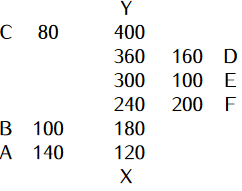
\includegraphics{images/MP1_Q18.png}

  a) Using a scale, draw an accurate map of the farm. \((3mks)\)

  b) Determine the actual area of the farm in hectares. \((4mks)\)

  c) If the farm is on sale at Ksh. 280,000 per hectare, find how much
  the farm costs.\((3mks)\)
\item
  Four ships are at sea such that a steam-liner W is 250 km on a bearing
  of \(030^0\) from a cargo ship Q. A trawler M is 350 km on a bearing
  of \(145^0\) from the cargo ship Q and a yacht R is due west of Q and
  on a compass bearing of \(N60^0W\) from M

  a) Using a scale of 1 cm=50 km, draw an accurate scale drawing showing
  the positions of W, Q, M, and R. \((5mks)\)

  b) By measurement from your scale drawing determine:

  i) The distance and bearing of R from W. \((3mks)\)

  ii) The distance WM. \((1mk)\)

  iii) The distance RM. \((1mk)\)
\item
  An electronics manufacturer makes speakers and sells them to a
  distributor at a profit of \(20\%\). The distributor sells the
  speakers to a retailer at a profit of \(25\%\). The retailer finally
  sells the speakers to customers at a profit of \(40\%\).

  a) A customer paid Ksh. 1,680 for a portable speaker. Find how much it
  had cost the manufacturer to make the speaker. \((3mks)\)

  b) A retailer bought a speaker which had cost the manufacturer Ksh.
  5,600 to make. Calculate the amount he paid for it. \((3mks)\)

  c) A customer bought a pioneer speaker at Ksh. 6,300. Calculate the
  much the distributor had paid for the same radio. \((2mks)\)

  d) Express as a percentage the amount the customer paid for the
  speaker in (c) above to the amount the distributor paid for it.
  \((2mks)\)
\item
  Four trucks A, B, C, and D are used to transport 42,000 bags of maize
  to a depot. However, trucks A and B together take 40 days to transport
  the same number of bags while trucks C and D together take 25 days.
  Truck A carries \(1\frac{1}{2}\) times the number of bags B carries
  and C carries \(1\frac{4}{5}\) times as much as D.

  a) Determine the number of bags of maize transported by each truck per
  day.\((5mks)\)

  b) All the trucks A, B, C, and D work together for 5 days, after which
  truck C and D are withdrawn. A and B work together for another 5 days
  after which truck A breaks down. How long does truck B take to
  complete the rest of the remaining bags? \((5mks)\)
\end{enumerate}

\end{tcolorbox}

\begin{tcolorbox}[enhanced jigsaw, left=2mm, colframe=quarto-callout-note-color-frame, toptitle=1mm, opacitybacktitle=0.6, rightrule=.15mm, colbacktitle=quarto-callout-note-color!10!white, colback=white, arc=.35mm, breakable, leftrule=.75mm, bottomtitle=1mm, bottomrule=.15mm, title=\textcolor{quarto-callout-note-color}{\faInfo}\hspace{0.5em}{Model Sample Paper 2}, titlerule=0mm, coltitle=black, toprule=.15mm, opacityback=0]

\ul{\textbf{SECTION A: (50 MARKS)}}

\textbf{Answer all the question in this section}

\begin{enumerate}
\def\labelenumi{\arabic{enumi}.}
\tightlist
\item
  Use the tables of squares and square roots only to find the value of;
  \((3mks)\)
\end{enumerate}

\[ \left(0.0847\right)^\frac{1}{2}+\left(2.35\right)^2\]

\begin{enumerate}
\def\labelenumi{\arabic{enumi}.}
\setcounter{enumi}{1}
\tightlist
\item
  Without using calculator, evaluate.\((3mks)\)
\end{enumerate}

\[\frac{2\frac{4}{5}+3\frac{1}{5}\div\frac{7}{8}\,of\,4\frac{4}{7}-\frac{3}{5}}{1\frac{3}{4}\div3\frac{1}{2}-\frac{5}{12}+\frac{2}{3}} \]

\begin{enumerate}
\def\labelenumi{\arabic{enumi}.}
\setcounter{enumi}{2}
\item
  Two years ago, Musa was three times as old as Ahmed. In four years'
  time, Musa will be twice as old as Ahmed. Find their present ages
  \((4mks)\)
\item
  On a map with a scale of 1:16,000, a banana plantation covers an area
  of \(70cm^2\). Find the area of the plantation in hectares. \((3mks)\)
\item
  A Canadian tourist came to Kenya with sterling pounds 4500 which he
  exchanged to Kenyan shillings. He spent a quarter of the money and
  exchanged the rest to sterling pounds on leaving. How much in sterling
  pounds did he receive? \((4mks)\)

  Exchange rate in Ksh. per pound
\end{enumerate}

\begin{verbatim}
           Buying          Selling
           119.74          119.88
              
\end{verbatim}

\begin{enumerate}
\def\labelenumi{\arabic{enumi}.}
\setcounter{enumi}{5}
\item
  The sums of interior angles of two regular polygons of sides' n-1 and
  n are in the ratio 3:4. Calculate;

  a) The value of n.~\((2mks)\)

  b) The size of interior angle of each polygon. \((2mks)\)
\item
  John bought six exercise books and three text books for Ksh. 660. If
  he had bought three similar exercise books and six text books, he
  would have paid Ksh. 210 more. How much would he pay for five exercise
  books and five text books? \((3mks)\)
\item
  Find the least number of biscuits that can be packed into carton boxes
  which contain either 4 or 9 or 24 or 40 with none left over.\((3mks)\)
\item
  In order to complete a certain job in 10 days, a company employs 30
  workers to work at the rate of 8 hours a day. Determine how long it
  would take 20 workers working at the rate of 12 hours a day to
  complete the same job. \((2mks)\)
\item
  Simplify the expression. \((3mks)\)
\end{enumerate}

\[\frac{y^2-4x-4xy+y}{(y+1)(4x^2-xy)}\]

\begin{enumerate}
\def\labelenumi{\arabic{enumi}.}
\setcounter{enumi}{10}
\item
  A two digit number is such that the sum of the ones and the tens digit
  is 11. If the Digits are reversed; the original number exceeds the new
  number formed by 9. Find the number. \((3mks)\)
\item
  Joyce on her cycling practice cycled on a bearing of \(125^0\) for
  5.5km, then on a bearing of \(180^0\) for 6.7km finally he turned
  northwards for 12.5km, by scale drawing determine the distance and
  compass bearing of her final position from the starting point.
  \((4mks)\)
\item
  Njoki bought Mike a suit for Ksh. 3600. This price was such that the
  shopkeeper had allowed a discount of 10\% on the marked price in order
  to make a profit of 20\%. Calculate both the marked price and the
  buying price of the suit. \((3mks)\)
\item
  Bronze is made by mixing tin, brass, and zinc in the ratio 3:5:4. A
  piece of bronze contains 7.2 kg of tin. Determine the total mass of
  brass and zinc in that piece of steel. \((2mks)\)
\item
  A cylindrical solid of length 40cm and radius 7cm is melted to form 10
  similar spherical solids. Determine the radius of each spherical
  solid. \((3mks)\)
\item
  Starting from midnight the minute hand of a clock moved so that the
  clock is showing 24 minutes past midnight.

  a) Find the angle through which the minute hand has moved. \((1mk)\)

  b) Given that the minute hand is 14 cm long, calculate the length of
  the arc it describes in that time. \((2mks)\)
\end{enumerate}

\ul{\textbf{SECTION B (50 MARKS)}}

\textbf{\emph{Attempt all the questions}}

\begin{enumerate}
\def\labelenumi{\arabic{enumi}.}
\setcounter{enumi}{16}
\item
  Simon sold an article at Ksh. 5,100 after allowing his customer a 15\%
  discount on the marked price of the article. In so doing he made a
  profit of 25\%.

  a) Calculate:

  i) The marked price of the article. \((2mks)\)

  ii) The price at which Simon had bought the article \((2mks)\)

  b) If Simon had sold the same article without giving a discount.
  Calculate the percentage profit he would have made to three
  significant figures. \((3mks)\)

  c) To clear his stock, Simon decided to sell the remaining articles at
  a loss of 20\%.Calculate the price at which he sold each article.
  \((3mks)\)
\item
  (a) Using a ruler and a pair of compasses only construct triangle ABC
  in which \(BC = 8cm\), \(AB = 6cm\) angle \(ABC = 67.5^0\) \((4mks)\)

  (b) Measure AC and angle ACB \((2mks)\)

  (c) Construct a circle that passes through AB, AC and BC \((3mks)\)

  (d) What is the radius of this circle? \((1mk)\)
\item
  A bus had 48 passengers at the begining of the journey, 20 passengers
  alighted at the first stop while 12 boarded. 8 of those who boarded at
  the first stop alighted at the second stop and 16 got in. The bus did
  not stop again upto the final destination. The charges from the
  starting point were Ksh. 100 upto the first stop, Ksh. 150 upto the
  second stop, and Ksh. 220 upto the final destination.

  a) How many passengers alighted at the final destination? \((3mks)\)

  b) How many passengers were ferried by the bus through the journey?
  \((2mks)\)

  c) How much money was collected during the trip? \((5mks)\)
\item
  (a) The angle of elevation of the top of a tree from a point P on the
  horizontal ground \(28.5^0\). From another point Q, five meters from P
  towards the base of the tree, the angle of elevation of the top of the
  tree is \(37.2^0\). By scale drawing calculate to one decimal place
  the height of the tree.\((4mks)\)

  (b) Four points A, B, C and D lie on the same plane. Point A is due
  southwest of point B. Point C is 70 Km on a bearing of \(S60^0E\) from
  B. Point D is equidistant from B, Q and C.

  i) Using the Scale: 1 cm represents 10km, construct a diagram showing
  the position of B, C, Q and D. \((4mks)\)

  ii) Determine the distance between A and B \((1mk)\)

  iii) Determine the bearing of D from B. \((1mk)\)
\item
  Water flows through a cylindrical pipe of diameter 2.8 cm at a speed
  of 70m/min.

  a) Calculate the volume of the water delivered by the pipe per minute
  in litres.\((3mks)\)

  b) A cylindrical storage tank of depth 5m is filled by water from this
  pipe and at the same rate of flow. Water begins flowing into the empty
  storage tank at 9.30 p.m. and is full by 2.10 a.m. Calculate the area
  of the cross-section of this tank in \(m^2\). \((4mks)\)

  c) A family consumes the capacity of this tank in one month. The cost
  of water is Ksh. 25 per thousand litres plus a fixed basic charge of
  Ksh. 1800.60. Calculate the cost of this family's water bill for the
  month. \((3mks)\)
\end{enumerate}

\end{tcolorbox}

\begin{tcolorbox}[enhanced jigsaw, left=2mm, colframe=quarto-callout-note-color-frame, toptitle=1mm, opacitybacktitle=0.6, rightrule=.15mm, colbacktitle=quarto-callout-note-color!10!white, colback=white, arc=.35mm, breakable, leftrule=.75mm, bottomtitle=1mm, bottomrule=.15mm, title=\textcolor{quarto-callout-note-color}{\faInfo}\hspace{0.5em}{Model Sample Paper 3}, titlerule=0mm, coltitle=black, toprule=.15mm, opacityback=0]

\ul{\textbf{SECTION A: (50 MARKS)}}

\textbf{Answer all the question in this section}

\begin{enumerate}
\def\labelenumi{\arabic{enumi}.}
\tightlist
\item
  Without using a calculator or mathematical tables, evaluate:
  \((3mks)\)
\end{enumerate}

\[\frac{15-6\times-14-21\div-3}{9\times3+-8(5-(-2))} \]

\begin{enumerate}
\def\labelenumi{\arabic{enumi}.}
\setcounter{enumi}{1}
\item
  Hannah finds that she needs 29 beacons placed 42 m apart when she
  surveys a length of road. If she was to place the beacons 49 m apart,

  a) How many beacons would she need? \((2mks)\)

  b) What is the shortest distance that can be divided into exact
  portions of 25, 30 or 40 metres giving a remainder of 3 metres.
  \((2mks)\)
\item
  Two friends Wakuraya and Muchoki have goats. Wakuraya has more goats
  than Muchoki and if Muchoki gives Wakuraya one of his goats, Wakuraya
  will have twice as many goats as Muchoki. If Wakuraya gives Muchoki
  one of his goat, they will have an equal number of goats. How many
  goats does each have.\((3mks)\)
\item
  Simiyu has six times as many one-shilling coins as twenty-shillings
  coins, a third as many five-shillings coins as one-shilling coins and
  four times as many ten-shillings coins as twenty-shilling coins. If in
  total he has Ksh. 228, find the number of coins he has. \((3mks)\)
\item
  The figure below shows the angles of a polygon ABCDE.

  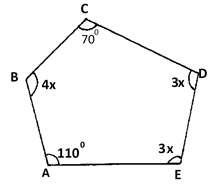
\includegraphics{figures/fig1.png}

  Obtain the size of each of the following angles,

  a) CBA \((2mks)\)

  b) CDE \((1mk)\)
\item
  The figure below is a cross-section of a swimming pool.

  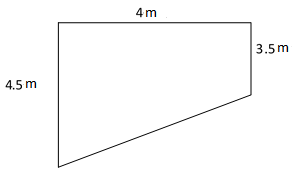
\includegraphics{figures/fig2.png}

  \begin{enumerate}
  \def\labelenumii{\alph{enumii})}
  \item
    Find the capacity of the pool in litres given that its length is
    27m. \((3mks)\)
  \item
    Given that the water has a density of \(1g/cm^3\), calculate the
    mass of water in the pool \((2mks)\)
  \end{enumerate}
\item
  Food aid 492,850 French Franc was donated to the Turkana drought
  stricken area. The food was purchased from United States of America
  (USA) and paid for in US dollars. Calculate the exact value of the
  food aid in dollars if: \((3mks)\)

  \(1\, French \, Franc = ksh \,12.80\,\) and
  \(\,1 \,Us \,dollars = ksh \,102.50\)
\item
  Munene is paid commission at the rate of 5 cents in every shilling on
  all goods he sells. During one month he sold 15 computers at Ksh.
  14,200 each, 6 DVD players at Ksh. 6,800 each and 8 laptops at Ksh.
  31,500 each. Calculate the total commission he earned in that month.
  \((3mks)\)
\item
  Sarah bought 3 plates and 6 jugs at a total cost of Ksh. 324. If she
  had bought 1 plate more and 2 jug less, she would have spent Ksh. 48
  less. On another occasion Sarah bought 5 plates and 5 jugs at the same
  prices. Find how much she spent on the second occasion. \((3mks)\)
\item
  A boat Q is 300m due west of boat P. Another boat R is 240m on a
  bearing of \(155^0\) from boat Q. Using scale drawing, find the
  distance ad bearing of boat R from P. \((4mks)\)
\item
  Two coils which are made by winding copper wire of different gauges
  and length have the same mass. The first coil is made by winding 250
  metres of wire with cross sectional diameter 2.1mm while the second
  coil is made by winding a certain length of wire with cross-sectional
  diameter 1.4mm. Find the length of wire in the second coil. \((3mks)\)
\item
  To prepare hay for the daily animals, green grass is dried and then
  processed into bails. In the process the mass of green grass decreases
  in the ratio 5:17. Determine the mass of green grass which must be
  processed to produce 1.2 tonnes of dry hay.\((3mks)\)
\item
  Evaluate using squares and square root tables. \((4mks)\)
\end{enumerate}

\[\left[\sqrt[]{27.47}+(0.701)^2 \right]^2\]

\begin{enumerate}
\def\labelenumi{\arabic{enumi}.}
\setcounter{enumi}{13}
\tightlist
\item
  Simplify: \((3mks)\)
\end{enumerate}

\[\frac{(4a+b)^2-(b-4a)^2}{(a+b)^2-(b-a)^2}\]

\begin{enumerate}
\def\labelenumi{\arabic{enumi}.}
\setcounter{enumi}{14}
\item
  The radius of a cylindrical tin is increased by \(24\%\) while its
  height is reduced by \(18\%\). In 4 significant figures find the
  percentage increase in the volume of the milk in the tin.\((3mks)\)
\item
  Taps A and B can fill a water tank in 40 minutes and 30 minutes
  respectively while C can empty in 20 minutes. If the three taps are
  turned on for 15 minutes then B and C closed. How long would it take
  before the tank is filled? \((3mks)\)
\end{enumerate}

\ul{\textbf{SECTION B (50 MARKS)}}

\textbf{\emph{Attempt all the questions}}

\begin{enumerate}
\def\labelenumi{\arabic{enumi}.}
\setcounter{enumi}{16}
\item
  A rectangular aluminum sheet whose density is \(2.2 g/cm^3\) is 1.2 m
  long, 80 cm wide, and 1.5 mm thick. A square of side 10 cm is cut off
  from each of the four corners of the rectangle and the remaining part
  folded into an open cuboid.

  a) Calculate:

  i) To the mass of the empty cuboid to the nearest Kg. \((4mks)\)

  ii) The capacity of the cuboid in litres \((2mks)\)

  b) If the cuboid is filled with alcohol whose density is
  \(0.75 g/cm^3\), calculate the mass of the cuboid when full of
  alcohol. \((4mks)\)
\item
  A bus left Dodoma on Thursday evening and traveled to Mombasa
  according to the travel table below and arrived there on Saturday
  morning.

  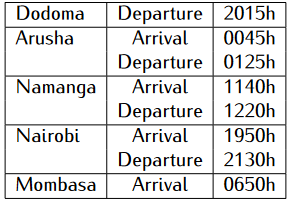
\includegraphics{figures/Md3_Q18.png}

  \begin{enumerate}
  \def\labelenumii{\alph{enumii})}
  \item
    Calculate the total:
  \item
    Travelling time for the whole journey. \((3mks)\)

    i. Stoppage time in all stations \((3mks)\)

    ii. Time taken for the whole journey \((2mks)\)
  \item
    Given that the average speed of the bus for the whole journey is
    60km/h, calculate the distance between Dodoma and Mombasa.
    \((2mks)\)
  \end{enumerate}
\item
  Three cargo ships P, Q, and R are at sea such that ship Q is 300 km on
  a compass bearing of \(N35^0W\) from ship P. ship R is 420 km on a
  bearing of \(220^0\) from ship Q. Another ship S is reported to be 475
  km from ship R and due south of ship P.

  a) Draw an accurate scale drawing showing the positions of ships P, Q,
  R, and S. (use scale 1cm=50 km) \((5mks)\)

  b) Use your scale drawing to determine the:

  i) Distance of ship S from P. \((1mk)\)

  ii) Distance and bearing of ship S from ship Q \((2mks)\)

  iii) Compass bearing of ship S from ship R \((2mks)\)
\item
  (a) A solution whose volume is 50 litres is made up of \(40\%\) water
  and \(60\%\) alcohol. When n litres of water are added the percentage
  of alcohol drops to \(50\%\). Find the value of n.~\((4mks)\)

  (b) 15 litres of water is added to the new solution. Calculate the
  percentage of alcohol in the resulting solution. \((2mks)\)

  (c) If 6 litres of the solution in (b) above is added to 3 litres of
  the original solution, calculate in the simplest form, the ratio of
  water to alcohol in the resulting solution. \((4mks)\)
\item
  Gabriel, an artisan made an article and sold it to a wholesaler to a
  profit of \(25\%\). The wholesaler sold it to a retailer at a profit
  of \(32\%\). The retailer finally sold the article to a customer at a
  profit of \(45\%\).

  a) If Gabriel used sh 1200 to make the article, find how much the
  customer paid for it. \((3mks)\)

  b) A customer paid sh 4785 for another article. Calculate how much the
  wholesaler had paid for it. \((3mks)\)

  c) During a clearance sale the retailer reduced his prices by
  \(20\%\). Find the percentage profit the retailer made on an article
  which had cost Gabriel sh 4000 to make it.\((4mks)\)
\end{enumerate}

\end{tcolorbox}

\begin{tcolorbox}[enhanced jigsaw, left=2mm, colframe=quarto-callout-note-color-frame, toptitle=1mm, opacitybacktitle=0.6, rightrule=.15mm, colbacktitle=quarto-callout-note-color!10!white, colback=white, arc=.35mm, breakable, leftrule=.75mm, bottomtitle=1mm, bottomrule=.15mm, title=\textcolor{quarto-callout-note-color}{\faInfo}\hspace{0.5em}{Model Sample Paper 4}, titlerule=0mm, coltitle=black, toprule=.15mm, opacityback=0]

\ul{\textbf{SECTION A: (50 MARKS)}}

\textbf{Answer all the question in this section}

\begin{enumerate}
\def\labelenumi{\arabic{enumi}.}
\tightlist
\item
  Evaluate without using a calculator or Mathematical tables leaving
  your answer in the simplest form. \((3mks)\)
\end{enumerate}

\[ \frac{\frac{3}{9}\,of\,\left(\frac{2}{5}-\frac{1}{10}\right)}{\left(4+\frac{2}{3}\right)\div\left(1+\frac{4}{3}\right)}\]

\begin{enumerate}
\def\labelenumi{\arabic{enumi}.}
\setcounter{enumi}{1}
\item
  Three similar 21 inch television sets and five similar 17 inch
  television cost Ksh. 145,000. The difference between the cost of two
  21 inch television sets and three 17 inch television Sets is Ksh.
  8,000. Calculate the price of a 21- inch television set and that of
  17-inch Television set. \((3mks)\)
\item
  A Kenya bank buys and sells foreign currencies as shown.
\end{enumerate}

\begin{verbatim}
                               Buying (Ksh)                   Selling (Ksh)
    1 Euro                      115.15                          115.26
    100 Japanese Yen             90.37                           90.45
    
\end{verbatim}

A Japanese traveling from France to Kenya had 4500 Euros. He converted
all the 4500 Euros to Kenya shilling at the bank. While in Kenya, he
spent a total of Ksh.225,600 and then converted the remaining Kenya
shilling to Japanese Yens at the bank. Calculate the amount in Japanese
Yen that he received. \((3mks)\)

\begin{enumerate}
\def\labelenumi{\arabic{enumi}.}
\setcounter{enumi}{3}
\tightlist
\item
  Use tables of square and square roots to evaluate.\((4mks)\)
\end{enumerate}

\[(0.3264)^2+\sqrt[]{364.5}\]

\begin{enumerate}
\def\labelenumi{\arabic{enumi}.}
\setcounter{enumi}{4}
\item
  A business woman usually makes a profit of \(32\%\) by selling a pair
  of shoes at sh 1650. If she reduces the price of the shoes by sh 250,
  calculate the percentage profit she will now make. \((3mks)\)
\item
  Kinyua bought soya and millet at Ksh.75 per kg and Ksh.45 per kg
  respectively. He then mixed them and sold the mixture at Ksh.65 per kg
  making a profit of \(30\%\). Determine the ratio of soya to millet in
  mixture. \((3mks)\)
\item
  The curved surface area of a cylindrical container is \(2540cm^2\). If
  the radius of the container is 28cm, calculate to one decimal place
  the capacity of the container in litres \((Take \pi=\frac{22}{7} )\).
  \((4mks)\)
\item
  The radius of a cylindrical tin is decreased by \(20\%\) while its
  height is increased by \(12\%\). In 4 significant figures find the
  percentage change in the volume of the milk in the tin and indicate
  whether it is an increase or a decrease. \((3mks)\)
\item
  Wang'ombe, a farmer, uses \(\frac{1}{2}\) of his land to plant
  cassava, \(\frac{1}{5}\) for planting sweet potatoes, \(\frac{1}{3}\)
  of the remainder for grazing and the rest for maize plantation. If he
  uses 10 hectares for grazing, determine how much land he uses for
  maize plantation. \((4mks)\)
\item
  Pauline bought 7 kg of rice and 3 KDF cakes at a total cost of Ksh.
  450. Wathitha bought 5 kg of rice and 8 KDF cakes at the same prices
  and spent Ksh. 70 less than Pauline. Calculate the cost of each item.
  \((3mks)\)
\item
  (a) Using a pair of compasses and a ruler only construct a triangle
  ABC such that \(AB = 6cm,\) \(BC = 8cm\) and \(ABC = 135^0\).
  \((2mks)\)

  (b) Construct the height of triangle ABC in (a) above taking BC as the
  base and measure the height. \((2mks)\)
\item
  One interior angle of a polygon is equal to \(40^0\) and each of the
  other interior angles are \(125^0\).Find the number of sides of the
  polygon. \((3mks)\)
\item
  Given that \(x=2\), \(y=-1\), and \(z=3\), find the value of;
  \((3mks)\)
\end{enumerate}

\[ \frac{5x^2-4y^2z+6y}{4x^2z+5y^3-z^3}\]

\begin{enumerate}
\def\labelenumi{\arabic{enumi}.}
\setcounter{enumi}{13}
\item
  Three boats X, Y, and Z are situated in such a way that boat Y is 450
  m on a compass bearing of \(S55^0E\) from boat X. Boat Z is 600 m on a
  bearing of \(035^0\) from boat Y.

  a) Draw a sketch showing the positions of X, Y, and Z. \((1mk)\)

  b) Calculate the distance of boat Z from boat X. \((2mks)\)
\item
  Pipe P can fill a tank in 6 minutes while pipe Q can fill the same
  tank in 10 minutes. On the other hand, a drainage pipe R, can empty
  the same full tank in 5 minutes. If Pipes P and Q are opened and left
  running for 3 minutes and then the drainage pipe R is then opened and
  all three left running, determine how many more minutes it takes to
  fill the drum. \((4mks)\)
\end{enumerate}

\ul{\textbf{SECTION B (50 MARKS)}}

\textbf{\emph{Attempt all the questions}}

\begin{enumerate}
\def\labelenumi{\arabic{enumi}.}
\setcounter{enumi}{15}
\item
  Mucagara secondary school hired a number of buses and matatus to ferry
  the students for an academic trip to Mombasa. The number of buses
  hired were two-third as many as matatus and no vehicle made a double
  trip. Each Matatu can carry a maximum of 18 students and a bus can
  carry three times as many students. The hire charges were Ksh. 8,400
  per bus and Ksh. 4,800 per matatu. A total of Ksh. 62,400 was spent on
  transport for the trip.

  a) Calculate the number:

  i) Of buses hired \((4mks)\)

  ii) Of matatus hired \((1mk)\)

  b) Calculate the number of students who took the trip if each vehicle
  was filled to capacity.\((3mks)\)

  c) Each student contributed Ksh 150 towards the cost of the trip and
  the school paid the remaining amount. Calculate the amount the school
  paid. \((2mks)\)
\item
  Three business dealers Kavula, Nzuki, and Ngina decided to buy a bus.
  They agreed to pay for the bus in the ratio 6:7:5. Using the marked
  price of the bus, Kavula was supposed to contribute Ksh. 120,600 more
  than Ngina. However, the sales agent allowed them a \(10\%\) discount
  after paying it on cash.

  a) Determine:

  i) The marked price of the bus. \((3mks)\)

  ii) The price at which they bought the bus. \((2mks)\)

  iii) How much more Kavula and Ngina paid than Nzuki? \((2mks)\)

  c) The dealers agreed that they would share monthly profits from the
  bus in the ratio of their contribution after setting aside \(10\%\) of
  the profits. If in one month the bus realized Ksh. 120,900 as the
  profit, how much did Ngina got? \((3mks)\)
\item
  A train left Nairobi on Monday evening and traveled to Mombasa
  according to the travel time table below. The train arrived in Lamu on
  Wednesday morning of the same week.

  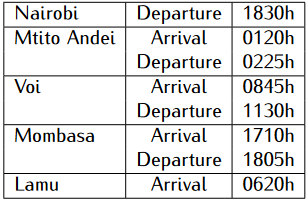
\includegraphics{figures/Md4_Q18.png}

  a) Calculate the time the train took to travel between: \((4mks)\)

  i) Nairobi and Mtito Andei

  ii) Mtito Andei and Voi

  iii) Voi and Mombasa

  iv) Mombasa and Lamu

  b) Determine the total time for the whole journey. \((4mks)\)

  c) Given that the railway road distance between Nairobi and Lamu is
  1505 Km, calculate the average speed for the whole journey. \((2mks)\)
\item
  The following measurements were recorded in a field book using XY as
  the base line. \(XY = 400m\).

  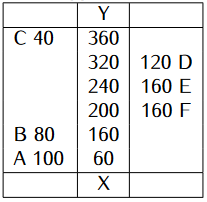
\includegraphics{figures/Md4_Q19.png}

  a) Using a scale of 1: 4000, draw an accurate map of the farm.
  \((4mks)\)

  b) Determine the actual area of the farm in hectares. \((4mks)\)

  c) If the farm is on sale at Ksh. 100,000 per hectare, find how much
  the farm costs. \((2mks)\)
\item
  Karani bought some eggs at Ksh 96 per dozen and sold three-quarter of
  them at Ksh 280 per tray and the remainder at Ksh 270 per tray. In so
  doing she made a profit of Ksh 675. Given that one tray holds 30 eggs,
  calculate:

  a) The number of eggs she bought. \((4mks)\)

  b) The percentage profit she made giving your answer to three
  significant figures. \((3mks)\)

  c) The percentage profit she would have made if she sold all the eggs
  at sh 280 per tray. \((3mks)\)
\end{enumerate}

\end{tcolorbox}

\begin{tcolorbox}[enhanced jigsaw, left=2mm, colframe=quarto-callout-note-color-frame, toptitle=1mm, opacitybacktitle=0.6, rightrule=.15mm, colbacktitle=quarto-callout-note-color!10!white, colback=white, arc=.35mm, breakable, leftrule=.75mm, bottomtitle=1mm, bottomrule=.15mm, title=\textcolor{quarto-callout-note-color}{\faInfo}\hspace{0.5em}{Model Sample Paper 5}, titlerule=0mm, coltitle=black, toprule=.15mm, opacityback=0]

\ul{\textbf{SECTION A: (50 MARKS)}}

\textbf{Answer all the question in this section}

\begin{enumerate}
\def\labelenumi{\arabic{enumi}.}
\tightlist
\item
  Evaluate. \((3mks)\)
\end{enumerate}

\[\frac{\left(32-(-16)\right)}{-8}-\frac{\left(18-(-)(-6)\right)}{3}\]

\begin{enumerate}
\def\labelenumi{\arabic{enumi}.}
\setcounter{enumi}{1}
\item
  The cost of 5 skirts and 3 blouses is Ksh. 1750. Afro's wife bought
  three skirts and one of the blouses for Ksh. 850. Find the cost of
  each item. \((3mks)\)
\item
  Last year, Gaceru was four times as old as his son, Kairu; in four
  years' time the sum of their ages will be 55. Determine their present
  ages. \((3mks)\)
\item
  Given that \(x=4\), \(y= -3\), and \(z= -1\) evaluate. \((3mks)\)
\end{enumerate}

\[\frac{3(x+z)^2-2(x-y)(y-z)}{3(x+z)-(y-z)}\]

\begin{enumerate}
\def\labelenumi{\arabic{enumi}.}
\setcounter{enumi}{4}
\item
  A plastic test tube is made up of hemispherical bottom and a
  cylindrical stem, both of internal radius 0.7cm.

  a) Calculate the capacity of the test tube, given that its height is
  12cm. \((3mks)\)

  b) Given that the test tube is filled with a liquid of density
  \(0.75 g/cm^3\), calculate the mass in g of the liquid in the test
  tube \((1mk)\)
\item
  A saleslady earns commission at the rate of 3.5 cents per shilling for
  all sales up to Ksh 350,000 and at the rate of 4.5 cents per shilling
  on any sales above that. During a certain month she sold 26 pieces of
  second hand computers at Ksh 14,500 per computer, 6 laptop batteries
  at Ksh. 4,500 each and 60 pieces of laptop chargers at Ksh 1,200 each.
  Calculate the total commission she earned in that month. \((3mks)\)
\item
  Water and milk are mixed such that the ratio of the volume of water to
  that of milk are 4:1. Taking the density of water as \(1g/cm^3\) and
  that of milk as \(1.25g/cm^3\), find the mass in grams of 2.4 litres
  of the mixture. \((3mks)\)
\item
  An arc of a circle of length 9.24cm subtends an angle of \(108^0\) at
  the centre of the circle. Calculate the area of the sector bounded by
  this arc. Take \(\pi=\frac{22}{7}\). \((3mks)\)
\item
  When maize seeds are dried up after harvest the mass decreases in the
  ratio 7:15. Find the mass of dried maize which is obtained after
  drying 1725 kg of green maize. \((3mks)\)
\item
  Bag X contains 672 sweets, bag Y 504 sweets and bag Z 360 sweets all
  of different types. The sweets are to be shared among a group of
  students in such a way each gets the same number of each type. Find
  the largest possible number of students.\((3mks)\)
\item
  On a map with a scale of \(1:50000\), a banana plantation covers an
  area of \(100\,cm^2\). Find the area of the plantation in hectares.
  \((3mks)\)
\item
  The radius of a cylindrical tin is increased by \(30\%\) while its
  height is decreased by \(25\%\). If the capacity of the old tin is
  \(400 cm^3\), find the capacity of the new tin. \((3mks)\)
\item
  Three towns P, Q, and R are such that tow Q is 90 km on a bearing of
  \(147^0\) from town P and town R is 120 km on a bearing of \(057^0\)
  from town Q.

  a) Draw a sketch showing the positions of the three towns. \((1mk)\)

  b) Calculate the distance between town P and R. \((2mks)\)
\item
  Find the exact value of: \((4mks)\)

  \(1.\dot{3}\dot{2}-0.5\dot{3}\)
\item
  Simplify the following expression by reducing it to a single fraction
  \((3mks)\)

  \[\frac{4a-5}{5}-\frac{2a-3}{3}=\frac{1-a}{6}\]
\item
  Starting from midnight the minute hand of a clock moved so that the
  clock is showing quarter to one.

  a) Find the angle through which the minute hand has moved. \((1mk)\)

  b) Determine the area of the sector described by the minute hand given
  that its length is 10.5 cm to 4 s.f. \((2mks)\)
\end{enumerate}

\ul{\textbf{SECTION B (50 MARKS)}}

\textbf{\emph{Attempt all the questions}}

\begin{enumerate}
\def\labelenumi{\arabic{enumi}.}
\setcounter{enumi}{16}
\item
  Using the linear equations below:

  a) Complete the tables below and then write down the point in
  coordinate form (x,y) as shown. \((4mks)\)

  \(2x+y=6\)

  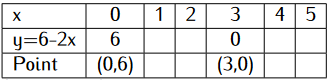
\includegraphics{figures/Md5_Q17a.png}

  \(3x-4y=9\)

  \includegraphics{figures/Md5_Q17b.png}

  b) Use graphical method by plotting the two linear equations on the
  same grid to solve the simultaneous equations: \((4mks)\)
\end{enumerate}

\begin{equation}
\begin{split}
2x+y&=6\\
3x-4y&=9
\end{split}
\end{equation}

\begin{enumerate}
\def\labelenumi{\alph{enumi})}
\setcounter{enumi}{2}
\tightlist
\item
  The line \(2x+y=6\) meets x-axis and the line y-axis at the points A
  and B respectively. From the graph state the co-ordinates of A and B.
  \((2mks)\)
\end{enumerate}

\begin{enumerate}
\def\labelenumi{\arabic{enumi}.}
\setcounter{enumi}{17}
\item
  A rectangular sheet measuring 80 cm by 50 cm and 2mm thick is made of
  copper whose density is \(2.5 g/cm^3\). A square of side 5 cm is
  removed from each corner of the rectangle and the remaining part
  folded to form an open cuboid.

  a) Calculate:

  i) The area of the copper which forms the cuboid.\((2mks)\)

  ii) The mass of the empty cuboid in Kilograms. \((4mks)\)

  b) If the cuboid is filled with water whose density is \(1 g/cm^3\),
  calculate the mass of the cuboid when full of water. \((4mks)\)
\item
  At 1400hr, two ships A and B leave port P and sail out to sea. Ship A
  sails at a steady speed of 55km/h on a bearing of \(060^0\) while ship
  B sails at a steady speed of 40km/h on a bearing of \(140^0\). At
  1800hr both ships radio back to port giving their positions. At the
  same time a third ship C gives its position as 300km due east of P.

  a) Using a ruler and a pair of compass only, construct a scale drawing
  showing the positions of P, A, B, and C at 1800hr. \((4mks)\)

  b) Use your scale drawing to determine:

  i) Distance and compass bearing of B from A \((4mks)\)

  ii) Distance of C from A \((2mks)\)

  iii) Distance Of B from C \((2mks)\)
\item
  In the year 2016 Muriithi had 40 more hens than cocks and half as many
  ducks as cocks. In the year 2017 his hens increased by \(60\%\), his
  ducks increased by \(40\%\) and his cocks decreased by \(20\%\). At
  the end of 2017 all his birds were 1335. Determine the percentage
  increase in the number of his birds in the year 2017. \((10mks)\)
\item
  (a) Using a ruler and a pair of compasses only, construct triangle
  \(ABC\) in which \(BC=6\) cm, \(AB=8.8\) cm and angle \(ABC=22.5^0\).
  \((4mks)\)

  (b) Measure AC and angle ACB. \((2mks)\)

  (c) Construct a circle that passes through A, B and C. \((3mks)\)

  (d) What is the radius of this circle? \((1mk)\)
\end{enumerate}

\end{tcolorbox}

\begin{tcolorbox}[enhanced jigsaw, left=2mm, colframe=quarto-callout-note-color-frame, toptitle=1mm, opacitybacktitle=0.6, rightrule=.15mm, colbacktitle=quarto-callout-note-color!10!white, colback=white, arc=.35mm, breakable, leftrule=.75mm, bottomtitle=1mm, bottomrule=.15mm, title=\textcolor{quarto-callout-note-color}{\faInfo}\hspace{0.5em}{Model Sample Paper 6}, titlerule=0mm, coltitle=black, toprule=.15mm, opacityback=0]

\ul{\textbf{SECTION A: (50 MARKS)}}

\textbf{Answer all the question in this section}

\begin{enumerate}
\def\labelenumi{\arabic{enumi}.}
\tightlist
\item
  Evaluate: \((3mks)\)
\end{enumerate}

\[\frac{8\times \frac{1}{3} \,of \,9\div 2-\frac{2}{3} \,of \,144 \div 12+2\times3}{\frac{3}{4} \,of\, 36 \div 3-4\div \frac{2}{5} of 10+3\times-2}\]

\begin{enumerate}
\def\labelenumi{\arabic{enumi}.}
\setcounter{enumi}{1}
\item
  Nyamu bought 5 pairs of trousers and 3 pairs of socks for sh 2,540. If
  the cost of three pairs of trousers and 5 pairs of socks is sh 1780,
  calculate the cost of two pairs of trousers and 6 pairs of socks.
  \((4mks)\)
\item
  Simplify: \((3mks)\)
\end{enumerate}

\[ \frac{(4a+b)^2-(b-4a)^2}{(a+b)^2-(b-a)^2}\]

\begin{enumerate}
\def\labelenumi{\arabic{enumi}.}
\setcounter{enumi}{3}
\item
  Taps P and Q can fill a water tank in 25 minutes and 20 minutes
  respectively while R can empty in 15 minutes. If the three taps are
  turned on for 12 minutes then Q and R closed. How long would it take
  before the tank is filled? \((3 mks)\)
\item
  The G.C.D of three numbers is 42 and their L.C.M is 1764. If two of
  the numbers are 84 and 294, what is the other smallest number?
  \((3 mks)\)
\item
  Gatungo sold a pullover to a customer for Ksh. 1240 after allowing her
  a 20\% discount on the marked price. Find the price at which the
  pullover was marked. \((2mks)\)
\item
  After harvesting the green maize, the seed are dried, treated and then
  packed in 70 kg bags. The mass of undried maize decreases in the ratio
  4:7. Calculate the mass of the undried maize that must be dried to
  produce 8 such bags when packed. \((3mks)\)
\item
  Hannah paid rent which was \(\frac{3}{10}\) of her net salary. She
  used \(\frac{1}{2}\) the remaining amount to make a down payment for a
  plot. She gave her mother Ksh. 3,200 and did shopping worth Ksh. 5,000
  for herself. She saved the remainder which was Ksh. 12,800. How much
  was the down payment that she made. \((4mks)\)
\item
  The interior angles of an hexagon are \((2x + 30)^0\),
  \((3x - 15)^0\), \((2x + 45)^0\), \(3x^0\), \((3x - 40)^0\) and
  \(x^0\). Find the value of the smallest exterior angle. \((3mks)\)
\item
  A Kenya company received y US Dollars. The money was converted into
  Kenya Shillings in a bank which buys and sells foreign currencies.
\end{enumerate}

\begin{verbatim}
                       Buying (in Ksh)        Selling (in (Ksh)
    1 Sterling Pound    125.78                  126.64 
    1 Us Dollar         102.66                  102.86
  
\end{verbatim}

\begin{enumerate}
\def\labelenumi{\alph{enumi})}
\item
  If the company received Ksh.12,452,658, calculate the amount, y
  received to the nearest US Dollar \((2mks)\)
\item
  The company exchanged the above Kenya shillings into Sterling pounds
  to buy a car in Britain. Calculate the cost of the car to the nearest
  Sterling pound. \((2mks)\)
\end{enumerate}

\begin{enumerate}
\def\labelenumi{\arabic{enumi}.}
\setcounter{enumi}{10}
\item
  item Juma, Ali and Hassan share the profit of their business in the
  ratio 2: 3: 5 respectively. If Juma receives ksh. 56, 000. How much
  profit did the hassan get. \((3mks)\)
\item
  Three police posts are such that Q is on a bearing of \(220^0\) and 14
  km from P while R is on a bearing of \(145^0\) and 10 km from P.

  a) Using a suitable scale, draw a diagram to represent the above
  situation. \((2mks)\)

  b) From the scale drawing determine:

  i) The distance and bearing of Q from R \((2mks)\)
\item
  Eighteen laborers takes 15 days to plough 6 acres of land. Find the
  number of laborers required to plough 8 acres in 12 days. \((2mks)\)
\item
  Starting from noon the minute hand of a clock moved so that the clock
  is showing 18 minutes to one.

  a) Find the angle through which the minute hand has moved. \((1mk)\)

  b) Given that the minute hand is 15 cm long, find the length of the
  arc it describes in that time. \((2mks)\)
\item
  Two coils of the same mass are made by winding brass wire of different
  gauges and length. If the first coil is made by winding 324 m of the
  wire with 3.36 mm cross-sectional diameter and the second coil is made
  by winding a certain length of the wire with a cross-sectional
  diameter of 2.52 mm, find the length of the second coil wire.
  \((3mks)\)
\item
  A Juakali artisan reduced the base radius of a cone shaped container
  by 15\% but, increased its height by 45\%. Find the in three s.f
  percentage change in its volume and state whether if the volume
  increased or decreased.(volume of a cone\(=\frac{1}{3}\pi r^2h\))
  \((3mks)\)
\end{enumerate}

\ul{\textbf{SECTION B (50 MARKS)}}

\textbf{\emph{Attempt all the questions}}

\begin{enumerate}
\def\labelenumi{\arabic{enumi}.}
\setcounter{enumi}{16}
\item
  From a reservoir, water flows through a cylindrical pipe of diameter
  0.3m at a rate of 0.28m per second.

  a) Determine the number of litres of water discharged from reservoir
  in one hour. \((4mks)\)

  b) The water flows from the reservoir for 15 hours per day for 22 days
  per month and serves a population of 3,000 families. Determine the
  average consumption of water per family per month giving your answer
  to the nearest 1 litres. \((4mks)\)

  c) The water is charged at the rate of Ksh. 10.50 per 100 litres.
  Calculate to the nearest Kenya shilling the average water in a family
  per month. \((2mks)\)
\item
  At noon, three ships P, Q, and R start together from port A and sail
  out to sea. Ship P sails at a steady speed of 40 km/h on a bearing of
  \(055^0\). Ship Q sails steadily at a speed of 60km/h due east of A
  and ship R sails steadily at 50km/h on a bearing of \(152^0\). At
  1530hr all three ships radio back to port giving their positions.

  a) Draw a sketch diagram showing the position of ships P, Q, and R at
  1500hr. \((1mk)\)

  b) Use a ruler and a pair of compasses only to construct a scale
  drawing showing the positions of the ships P, Q, and R with respect to
  port A at 1500 hrs (1cm=25km). \((5mks)\)

  c) By measurement use your scale drawing to determine:

  i) The distance and bearing of ship P from ship Q. \((2mks)\)

  ii) The distance of ship R from ship Q. \((1mk)\)

  iii) The distance of ship P from ship R. \((1mk)\)
\item
  (a) A small field was surveyed and the measurements recorded in a
  surveyor's field book as in the table below.

  \includegraphics{figures/Md6_Q19a.png}

  Using a scale of 1cm to 15 m make an accurate drawing of the map of
  the field. \((4mks)\)

  (b)

  i) Find the area of the field. \((3mks)\)

  ii) Assuming that the baseline in (a) runs in a northern direction
  give the position of D relative to A using compass bearing and
  distance. \((3mks)\)
\item
  Four trucks A, B, C and D are used to transport 27,000 bags of maize
  to a depot. However, trucks A and B together take 24 days to transport
  the same number of bags while trucks C and D together take 15 days.
  Truck A carries \(1\frac{1}{4}\) times the number of bags B carries
  and C carries \(1\frac{2}{5}\) times as much as D.

  a) Determine the number of bags of maize transported by each truck per
  day. \((5mks)\)

  b) All the trucks A, B C and D work together for 5 days, after which
  truck C and D are withdrawn. A and B work together for another 5 days
  after which truck A breaks down. How long does truck B take to
  complete the rest of the remaining bags? \((5mks)\)
\item
  A solution whose volume is 160 litres is made up of \(40\%\) water and
  the rest alcohol. When x litres of water is added the percentage of
  alcohol drops to \(30\%\)

  a) Find the value of x \((4mks)\)

  b) If 1 litres of alcohol are added to the new solution, calculate the
  percentage of water in the resulting solution. \((2mks)\)

  c) A blend is made by mixing 25 litres of the solution in (b) above
  with 20 litres of the original solution. Calculate in the simplest
  form, the ratio of water to that of alcohol in the blend. \((4mks)\)
\end{enumerate}

\end{tcolorbox}

\begin{tcolorbox}[enhanced jigsaw, left=2mm, colframe=quarto-callout-note-color-frame, toptitle=1mm, opacitybacktitle=0.6, rightrule=.15mm, colbacktitle=quarto-callout-note-color!10!white, colback=white, arc=.35mm, breakable, leftrule=.75mm, bottomtitle=1mm, bottomrule=.15mm, title=\textcolor{quarto-callout-note-color}{\faInfo}\hspace{0.5em}{Model Sample Paper 7}, titlerule=0mm, coltitle=black, toprule=.15mm, opacityback=0]

\ul{\textbf{SECTION A: (50 MARKS)}}

\textbf{Answer all the question in this section}

\begin{enumerate}
\def\labelenumi{\arabic{enumi}.}
\tightlist
\item
  Evaluate \((3mks)\)
\end{enumerate}

\[\frac{1\frac{1}{4}\,of\,20+3\frac{3}{4}\div \frac{3}{8}-4\frac{1}{2}\times3\frac{1}{3}}{5\frac{4}{9}\times1\frac{2}{7}-4\div \frac{2}{3}+\frac{3}{4}\,of\,12}\]

\begin{enumerate}
\def\labelenumi{\arabic{enumi}.}
\setcounter{enumi}{1}
\tightlist
\item
  Use squares and square root tables to evaluate. \((4mks)\)
\end{enumerate}

\[ (0.9233)^2+\sqrt[]{15.2453}-0.223\]

\begin{enumerate}
\def\labelenumi{\arabic{enumi}.}
\setcounter{enumi}{2}
\item
  A UK tourist comes to Kenya with \(\pounds, 65, 000\). He pays
  \(25\%\) commission at the airport and his expenses in Kenya amounted
  to Ksh. 890,000. How much money did he remain with in Ksh? (Take
  \(1\, UK \pounds = Ksh. 130.50\)) \((3mks)\)
\item
  All prime numbers less than 10 are arranged in a descending order to
  form a number which forms a quotient of 1883 with a certain number.
  Calculate the number \((3mks)\)
\item
  Solve the equation \((2mks)\)
\end{enumerate}

\[\frac{1}{2y}=\frac{3}{4y+1}\]

\begin{enumerate}
\def\labelenumi{\arabic{enumi}.}
\setcounter{enumi}{5}
\item
  Daniel deposited 48 different notes in the bank. He had eight times as
  many two-hundred shilling notes as one-thousand shilling notes and
  half as many one-hundred shilling notes as two-hundred shilling notes.
  The rest were fifty shilling notes. If he deposited a total of Ksh.
  9,450, find the number of fifty shilling notes he deposited.
  \((3mks)\)
\item
  Esther bought maize and sorghum flour from a vendor. She then mixed
  them in the ratio 4:3. She bought the maize flour at ksh.50 per kg and
  the millet flour at ksh. 71 per kg. If she was to sell and make a
  profit of \(25\%\). What should be the selling price of 1kg of the
  mixture? Give you answer correct to the nearest 10 cent. \((3mks)\)
\item
  Teresia sold a dress at Ksh. 1,290 after allowing a discount of Ksh.
  160. If she did not allow any discount to the customer, she would have
  made a profit of \(25\%\). Calculate the percentage profit she made.
  \((3mks)\)
\item
  Nyambura bought 4 sufurias and 6 cups for Ksh. 850 from a hawker. If
  she had bought 3 sufurias and 9 cups she would have saved Ksh. 55.
  Calculate the cost of one sufuria. \((3mks)\)
\item
  Omondi is now two-third as old as his sister and twice as old as his
  younger brother. In six years' time Omondi's age will be 26 years less
  than the sum of ages of his sister and brother. Determine Omondi's
  present age. \((3mks)\)
\item
  A Juakali artisan reduced the base radius of a cone shaped container
  by \(15\%\) but, increased its height by \(45\%\). Find the in three
  s.f percentage change in its volume and state whether if the volume
  increased or decreased (volume of a cone \(=\frac{1}{3}\pi r^2h\)
  \((3mks)\)
\item
  The sum of the interior angles of an n-sided polygon is \(720^0\).
  Find the value of n and hence give the name of the polygon. \((3mks)\)
\item
  A rectangular water tank has a base measuring 4.5m by 2m. This tank
  has water to a height of 90cm. Water is then pumped into this tank
  continuously from 2030 hours to 2140 hours at the rate of 1.2 litres
  per second. Find the new depth of water in the tank after this period
  of time giving your result in metres. \((3mks)\)
\item
  Four strings measuring 15cm, 20cm, 25cm and 30cm are cut into pieces
  of equal length so that exact number of pieces is obtained from each
  string without wastage. Find the longest length of each string.
  \((2mks)\)
\item
  The number of students at Lorna Waddington High School is 600. On a
  particular day \(\frac{1}{5}\) of the boys and \(\frac{1}{4}\) of the
  girls attended a sports meeting. If 468 students were left behind,
  find how many more boys than girls attended the meeting. \((4mks)\)
\item
  Using ruler and a pair of compasses only:

  i) Construct triangle ABC in which BC = 7.5 cm and angle
  \(ABC = 105^0\) and angle \(BAC = 30^0\). \((3mks)\)

  ii) Drop a perpendicular from A to meet line BC at P. Determine the
  area of triangle ABC. \((2mks)\)
\end{enumerate}

\ul{\textbf{SECTION B (50 MARKS)}}

\textbf{\emph{Attempt all the questions}}

\begin{enumerate}
\def\labelenumi{\arabic{enumi}.}
\setcounter{enumi}{16}
\item
  A protestant church hired a number of buses and matatus to transport a
  group of youths to Embu for a youths rally. The number of matatus was
  four times the number of buses. The hire charges were Ksh. 5,200 per
  matatu and Ksh. 9,000 per bus. The total cost of hiring the vehicles
  was Ksh. 59,600. Each matatu can carry 14 youths while a bus can carry
  three times as many.

  a) Calculate:

  i) The number of buses hired \((4mks)\)

  ii) The number of matatus hired \((1mk)\)

  b) Calculate the number of youths ferried to Embu if each vehicle was
  filled to capacity and no vehicle made a double trip. \((3mks)\)

  c) Each youth contributed Ksh. 200 towards the cost of the trip and
  the church paid the remaining amount. How much did the church pay?
  \((2mks)\)
\item
  Three business partners Muhammed, Maimuna , and Hasan decided to start
  a business. Muhammed contributed Ksh. 25,000, Maimuna contributed Ksh.
  35,000, and Hasan contributed Ksh. 45,000 as business capital
  exclusive of rental fee. They rented a business premises that needed
  to be paid Ksh. 15,000 which was to be shared equally among them. They
  agreed to put \(25\%\) of the profit obtained annually back in to the
  business and share the rest in the ratio of their contributions. The
  business realized Ksh. 128,000 as gross profits.

  a) Find the ratio in which they contributed business capital and
  rental fees. \((3mks)\)

  b) Calculate:

  i) The profits shared. \((2mks)\)

  ii) Each partner's share of the profits. \((3mks)\)

  iii) The percentage of Hasan share to the sum of Maimuna and Muhammed
  share. \((2mks)\)
\item
  In 2008, the number of students in Mucagara Secondary School was 240,
  a \(20\%\) increase over the number of students in 2007. The number of
  students dropped by \(5\%\) in 2009 but, increased by \(25\%\) in the
  year 2010.

  a) Determine the number of students:

  i) In the year 2007 \((2mks)\)

  ii) In the year 2009 \((2mks)\)

  iii) In the year 2010 \((2mks)\)

  b) Express as a percentage the increase in the number students in the
  year 2010 over the that in the year 2008 \((2mks)\)

  c) What was the percentage increase in student population between 2007
  and 2009. \((2mks)\)
\item
  Use the given linear equations to:

  a) Complete the table below \((4mks)\)

  \(3x+y=9\)

  \includegraphics{figures/Md7_Q20a.png}

  \(x-2y=-4\)

  \includegraphics{figures/Md7_Q20b.png}

  b) Using graph solve the simultaneous equations: \((4mks)\)
\end{enumerate}

\begin{equation}
\begin{split}
x-2y&= -4\\
3x+y&=9
\end {split}
\end{equation}

\begin{enumerate}
\def\labelenumi{\alph{enumi})}
\setcounter{enumi}{2}
\tightlist
\item
  If the line \(3x+y= 9\) cuts the x-axis and y-axis at A and B
  respectively, state the coordinates of A and B. \((2mks)\)
\end{enumerate}

\begin{enumerate}
\def\labelenumi{\arabic{enumi}.}
\setcounter{enumi}{20}
\item
  A Parrot flies from a tree X to another tree Y which is 70m on a
  bearing of \(035^0\) from X. From Y the dove flies 100 m due west to
  another tree Z and finally flies due south to another tree W which is
  on a bearing of \(230^0\) from X.

  a) Using a ruler and a pair of compasses only construct an accurate
  scale drawing showing the positions of X, Y, Z, and W. (scale : 1
  cm=10 cm) \((4mks)\)

  b) By measurement from your scale drawing determine:

  i) The distance and bearing of Z from X. \((2mks)\)

  ii) The distance of W from Z \((1mk)\)

  iii) The distance of W from X \((1mk)\)

  c) The compass bearing of W from Y. \((2mks)\)
\end{enumerate}

\end{tcolorbox}

\begin{tcolorbox}[enhanced jigsaw, left=2mm, colframe=quarto-callout-note-color-frame, toptitle=1mm, opacitybacktitle=0.6, rightrule=.15mm, colbacktitle=quarto-callout-note-color!10!white, colback=white, arc=.35mm, breakable, leftrule=.75mm, bottomtitle=1mm, bottomrule=.15mm, title=\textcolor{quarto-callout-note-color}{\faInfo}\hspace{0.5em}{Model Sample Paper 8}, titlerule=0mm, coltitle=black, toprule=.15mm, opacityback=0]

\ul{\textbf{SECTION A: (50 MARKS)}}

\textbf{Answer all the question in this section}

\begin{enumerate}
\def\labelenumi{\arabic{enumi}.}
\tightlist
\item
  Evaluate: \((3mks)\)
\end{enumerate}

\[ \frac{6\times\frac{1}{3}\,of\,12\div2-\frac{1}{3}\,of\,36\div6+3\times4}{\frac{1}{4}\,of\,24\div2-24\div\frac{3}{5}\,of\,10+5\times(-2)}\]

\begin{enumerate}
\def\labelenumi{\arabic{enumi}.}
\setcounter{enumi}{1}
\item
  Factorize completely \((3mks)\)

  \[(x+y)(4x-5y)-(x+y)^2\]
\item
  Murimi, a cattle keeping farmer, has twenty five times as many cows as
  goats, and three-fifth as many sheep as goats.

  a) If there are g goats, write down a simplified expression in g for
  the total number of animals Murimi has. \((1mk)\)

  b) Given that there are 75 sheep, calculate as a percentage the sum of
  goats and sheep to the number of cows Murimi had. \((3mks)\)
\item
  Four interior angles of a hexagon are \(120^0\), \(115^0\), \(135^0\)
  and \(80^0\). The fifth interior angle is twice times the sixth. Find,
  in degrees the sixth interior angle. \((3mks)\)
\item
  Munyiti uses \(\frac{1}{3}\) of his farm for planting mangoes,
  \(\frac{1}{4}\) for planting macadamia and \(\frac{2}{5}\) of the
  remainder for grazing and home stead. He still has 6 hectares of
  unused land. Find the size of land Munyiti used for planting
  mangoes.\((3mks)\)
\item
  Use tables and squares roots to evaluate to 4 significant figures.
  \((4mks)\)
\end{enumerate}

\[\left(\sqrt[]{245.6}+(4.436)^2\right)^\frac{1}{2}\]

\begin{enumerate}
\def\labelenumi{\arabic{enumi}.}
\setcounter{enumi}{6}
\item
  A speaker coil which is made by winding 750 m of copper wire of
  cross-sectional diameter of 1.89 mm has the same mass as another coil
  of copper wire with cross-sectional diameter of 2.1 mm. Find the
  length of the wire making the second coil. \((3mks)\)
\item
  Three children shared some money. Rose got \(0.\dot{5}\) of the money
  and Mutua \(0.\dot3\) of the remainder. Loice received the rest which
  was Ksh. 400. How much did Mutua get? \((4mks)\)
\item
  The sum of the interior angles of an n-sided polygon is \(1080^0\).
  Find the value of n and hence calculate the size of each exterior
  angle. \((3mks)\)
\item
  Three metal rods of lengths 243cm, 270cm and 198cm were cut into
  shorter pieces all of the same length to make window grills. Calculate
  the length of the longest piece that can be cut from each of the rods
  and hence the total number of pieces that can be obtained from the
  rods. \((3mks)\)
\item
  A blend of juice is made from pineapple and passion. The cost of two
  limes of pineapple is Ksh. 162 and three limes of passion is Ksh. 414.
  In what ratio should the juice be mixed such that by selling the
  mixture at Ksh. 140 per lime a profit of \(40\%\) is realized?
  \((3mks)\)
\item
  Awino bought a shirt for Ksh. 1400 and sold it to a customer at a
  profit of \(35\%\). What is the marked price of the shirt if selling
  the shirt she had allowed her customer a \(10\%\) discount on the
  marked price? \((4mks)\)
\item
  Sarah bought 3 plates and 6 jugs at a total cost of Ksh. 324. If she
  had bought 1 plate more and 2 jug less, she would have spent Ksh. 48
  less. On another occasion Sarah bought 5 plates and 5 jugs at the same
  prices. Find how much she spent on the second occasion. \((3mks)\)
\item
  A Kenyan tourist left Berlin, Germany for Nairobi, Kenya through
  Geneva, Switzerland. While in Geneva, he bought a watch worth 110.6
  Deutsche marks. Using the exchange rates below:
\end{enumerate}

\begin{verbatim}
1 Swiss Franc = 1.58 Deutsche marks.

1 Swiss Franc = 100.98 Kenya shillings.
\end{verbatim}

\begin{enumerate}
\def\labelenumi{\arabic{enumi}.}
\setcounter{enumi}{14}
\item
  Find the value of the watch in:

  a) Swiss Francs \((2mks)\)

  b) Kenya shillings \((1mk)\)
\item
  Using a ruler and a pair of compasses only construct triangle ABC such
  that \(AB= 5.8\,cm\), \(BC = 7\,cm\) and angle \(CBA = 75^0\). Measure
  angle \(CAB\). \((3mks)\)
\item
  Two pipes A and B each running alone can fill a Jerican in 6 hours and
  10 hours respectively. a drainage pipe C can empty the full Jerican in
  15 hours. If pipe A and B are turned on and left running for
  \(1\frac{1}{2}\) hours and then the drainage pipe C is opened and all
  three left running, find how much longer it takes to fill the Jerican.
  \((4mks)\)
\end{enumerate}

\ul{\textbf{SECTION B (50 MARKS)}}

\textbf{\emph{Attempt all the questions}}

\begin{enumerate}
\def\labelenumi{\arabic{enumi}.}
\setcounter{enumi}{17}
\item
  Peter bought a second hand probox and later sold it through a sales
  agent who charges \(6.5\%\) commission on the price of the probox. He
  received Ksh. 392,700 from the agent after the latter had deducted his
  commission. Peter incurred a loss of \(30\%\) on the price at which he
  had bought the probox.

  a) Determine the price at which the agent sold the probox. \((2mks)\)

  b) Find the price at which Peter had bought the probox \((3mks)\)

  c) If the amount Peter paid for the probox was \(25\%\) less than the
  price of the new probox, calculate the price of the new probox.
  \((3mks)\)

  d) Express as a percentage the amount Peter received for his probox to
  its price when new. \((2mks)\)
\item
  Nyakio and Anyango went to buy clothes for their business. Nyakio
  spent Ksh. 20,150 to buy a number of dresses and skirts from a
  wholesaler A at Ksh. 450 per dress and Ksh. 200 per skirt. Anyango
  bought the same number of dresses and skirts from wholesaler B where
  she paid \(20\%\) less per dress and \(10\%\) more per skirt. It was
  found that Anyango spent Ksh. 2,710 less than Nyakio.

  a) Determine the number of dresses and skirts each cloth dealer
  bought.\((4mks)\)

  b) Nyakio sold all her clothes at a profit of \(20\%\) per dress and
  \(40\%\) per skirt. How much profit did she make? \((3mks)\)

  c) Anyango also sold all her clothes at a profit of \(20\%\) per dress
  and \(40\%\) per skirt. Calculate to three significant figures the
  percentage profit she made. \((3mks)\)
\item
  A metal sheet measuring \(1 \,m\) long and \(80 \,cm\) wind is
  \(2\,mm\) thick and its density is \(2.5 g/cm^3\). A square of side
  \(x\, cm\) is removed from each of the four corners and the remaining
  part folded to form an open cuboid.

  a) Calculate the area of the remaining part in terms of \(x\).
  \((2mks)\)

  b) Given that the area of the remaining part is \(0.76 \,m^2\),
  calculate the value of \(x\) and hence state the internal dimensions
  of the cuboid.\((3mks)\)

  c) Calculate the mass in kg of the empty cuboid to two significant
  figures.\((2mks)\)

  d) If the cuboid is filled with a liquid of density \(d \,g/cm^3\) and
  its mass when full of the liquid is 39.8 kg, calculate the value of
  \(d\).\((3mks)\)
\item
  Use a ruler and a pair of compasses only for all the constructions in
  this question.

  a) Construct a triangle \(ABC\) in which \(BC=7cm\), \(AC=9cm\), and
  angle \(ACB=135^0\) \((3mks)\)

  b) Measure AB and angle ABC \((2mks)\)

  c) From A drop a perpendicular to meet BC produced at D. \((1mk)\)

  d) Measure AD and hence calculate the area of triangle ABC. \((2mks)\)

  e) Mark a point E on AD such that area of triangle BEC is 1.5 the area
  of triangle ABC. \((1mk)\)

  f) Complete triangle BEC and measure EC. \((1mk)\)
\item
  Town B is 250 km from a bearing of \(050^0\) from town A. Town C is
  350 km from town B and on a compass bearing of \(S57^0E\) from town B.
  A fourth town D is on a bearing of \(240^0\) from town C and due south
  of town A.

  a) Using a scale of \(1\,cm=50 \,km\), draw an accurate scale drawing
  showing the positions of towns A, B, C, and D. \((5mks)\)

  b) By measurement from your scale drawing, determine:

  i) The distance AC \((1mk)\)

  ii) The distance AD \((1mk)\)

  iii) The distance CD \((1mk)\)

  iv) The bearing of B from C \((2mks)\)
\end{enumerate}

\end{tcolorbox}

\begin{tcolorbox}[enhanced jigsaw, left=2mm, colframe=quarto-callout-note-color-frame, toptitle=1mm, opacitybacktitle=0.6, rightrule=.15mm, colbacktitle=quarto-callout-note-color!10!white, colback=white, arc=.35mm, breakable, leftrule=.75mm, bottomtitle=1mm, bottomrule=.15mm, title=\textcolor{quarto-callout-note-color}{\faInfo}\hspace{0.5em}{Model Sample Paper 9}, titlerule=0mm, coltitle=black, toprule=.15mm, opacityback=0]

\ul{\textbf{SECTION A: (50 MARKS)}}

\textbf{Answer all the question in this section}

\begin{enumerate}
\def\labelenumi{\arabic{enumi}.}
\tightlist
\item
  Evaluate: \((3mks)\)
\end{enumerate}

\[\frac{\frac{3}{5}\,of\,30+5\frac{5}{6}\div\frac{7}{12}-2\frac{2}{3}\times 1\frac{1}{2}}{5\frac{5}{8}\times1\frac{7}{9}-1\frac{1}{4}\,of\,4\frac{4}{5}+2\frac{4}{5}\div\frac{7}{10}}\]

\begin{enumerate}
\def\labelenumi{\arabic{enumi}.}
\setcounter{enumi}{1}
\item
  A law firm bought 60 files at a total cost of Ksh. 10,000. Some files
  cost Ksh. 150 each while others cost Ksh. 250 each. Find the number of
  files which were bought at Ksh. 150 each. \((3mks)\)
\item
  Mutheu is now 10 years older than her younger brother. Six years ago
  the She was three times as old as his brother. Find their present
  ages. \((3mks)\)
\item
  Wambui marked a skirt at Ksh. 400 and sold it to a customer at a
  discount of \(15\%\). Find the percentage profit She made if she had
  bought the skirt at Ksh. 280. \((3mks)\)
\item
  Use tables to evaluate:- \((4mks)\)
\end{enumerate}

\[(6.342+3.289)^2-\sqrt[]{(432.85-124.45)}\]

\begin{enumerate}
\def\labelenumi{\arabic{enumi}.}
\setcounter{enumi}{5}
\item
  Osinya constructed a closed wooden box with external measurements 1.5
  metres long, 1.4 metres wide and 0.6 metres high. The wood used in
  constructing the box was 10.0cm thick and has a density of
  \(0.75g/cm^3\). Determine the:

  a) Volume in \(cm^3\) of the wood used in constructing the box.
  \((3mks)\)

  b) Mass of the box in kilograms correct to 1 decimal place. \((1mk)\)
\item
  Factorize completely \((3mks)\)

  \[(x-3y)(4x+3y)-(x-3y)^2\]
\item
  16 workers working at the rate of 9 hours a day can complete a piece
  of work in 14 days. How many more workers working at the rate of 7
  hours a day wound complete the same job in 12 days. \((3mks)\)
\item
  In a form one class there are 5 more boys than girls. On a certain day
  one-quarter of the boys and one-fifth of the girls went for a football
  games. If 8 students from this class went for the football game, find
  the number of students in the class. \((3mks)\)
\item
  Kamau toured Switerland from Germany. In Switzerland he bought his
  wife a present worth 150 Deutsche marks. If

  1 Swiss Franc = 1.65 Deutsche marks

  1 Swiss Franc = 100.90 Kenya shillings

  Find the value of the present in:

  a) Swiss Francs correct to 2 decimal places. \((1mk)\)

  b) Kenya shillings correct to the nearest Ksh \((2mks)\)
\item
  Find the least number of biscuits that can be packed into carton boxes
  which contain either 10 or 15 or 21 or 24 with leaving 5 biscuits
  unpacked. \((3mks)\)
\item
  A polygon of n sides has half of the interior angles \(140^0\) each
  and the rest \(160^0\) each. Find the value of n.~\((2mks)\)
\item
  A coffee dealer mixes two brands of coffee, P and Q to obtain 50kg of
  the mixture worth Ksh. 60. If brand P is valued at Ksh. 80 per kg and
  brand Q is valued at Ksh. 50 per kg. Calculate the ratio in its
  simplest form in which brands P and Q are mixed. \((4mks)\)
\item
  In a 3 digit number, the hundreds digits is 3 more than the units
  digit and the tens digit is thrice the hundreds digit. If the sum of
  the digits is 12, find the three digits. Write the number. \((3mks)\)
\item
  Three similar pieces of timber of length 150cm, 140cm and 180cm are
  cut into equal pieces. Find the largest possible area of a square
  which can be made from any of the three pieces. \((3mks)\)
\item
  Arrange the following fractions in descending order. \((3mks)\)
\end{enumerate}

\[ \frac{3}{5},\frac{8}{9},\frac{1}{3},\frac{4}{7},\frac{3}{4}\]

\ul{\textbf{SECTION B (50 MARKS)}}

\textbf{\emph{Attempt all the questions}}

\begin{enumerate}
\def\labelenumi{\arabic{enumi}.}
\setcounter{enumi}{16}
\item
  Melvin bought a second hand minibus at later sold it through a sales
  agent who charged \(8\%\) commission on the price at which she sold
  the minibus. She received Ksh. 699,200 from the agent after she had
  deducted her commission. Melvin made a profit of \(15\%\) on the price
  at which she had bought the vehicle.

  a) Calculate the price at which the sales agent sold the minibus.
  \((2mks)\)

  b) Find the amount Melvin paid for the minibus. \((3mks)\)

  c) If the amount Melvin paid was 50\% less than the price of the new
  minibus, calculate its price when new. \((3mks)\)

  d) Express as a percentage the amount Melvin received for the minibus
  to its price when new. \((2mks)\)
\item
  Given linear equations \(2x+y=7\) and \(5x-3y=12\):

  a) Complete the following tables: \((4mks)\)

  \(2x+y=7\)

  \includegraphics{figures/Md9_Q18a.png}

  \(5x-3y=12\)

  \includegraphics{figures/Md9_Q18b.png}

  b) Use graphical method to solve the simultaneous equations:
  \((4mks)\)

  \begin{equation}
  \begin {split}
  2x+y&=7\\
  5x-3y-12&=0
  \end{split}
  \end{equation}

  c) If the line \(2x+y-7=0\) cuts x-axis and y-axis at point A and B
  respectively, state the coordinates of A and B. \((2mks)\)
\item
  (a) Solution whose volume is 100 litres is made up of \(30\%\) water
  and \(70\%\) milk. When y litres of water are added the percentage of
  milk drops to \(40\%\). Find the value of y. \((4mks)\)

  (b) Twenty five litres of water is added to the new solution.
  Calculate the percentage of milk in the resulting solution. \((2mks)\)

  (c) If 8 litres of the solution in (b) above is added to 16 litres of
  the original solution, calculate in the simplest form, the ratio of
  water to milk in the resulting solution. \((4mks)\)
\item
  Kiptanui's farm produced 13,600 bags of wheat in 2015 which was a
  decrease of \(15\%\) over the production in 2014. In 2016, the
  production was a \(25\%\) increase of the previous year but, in 2017
  Kiptanui farm produced 16,405 bags of wheat.

  a) Calculate the number of bags of wheat Kiptanui's farm produced:

  i) In 2014 \((2mks)\)

  ii) In 2016 \((2mks)\)

  b) What was the percentage decrease in production in 2017 over that of
  the previous year? \((2mks)\)

  c) Determine the percentage increase in production in 2017 over that
  in 2014. Give your answer in 3 significant figure \((2mks)\)

  d) Calculate the percentage increase in production in 2016 over that
  in 2014. \((2mks)\)
\item
  The external measurements of a closed wooden box are 1.0 m long, 70 cm
  wide, and 40 cm high. The wood used in making the box is 1.5 cm thick
  and has a density of \(0.8 g/cm^3\). Given that the box contains 25
  packets of tools and each packet holds a dozen tools each weighing
  108.5 g, calculate:

  a) The volume of wood used in making the box. \((4mks)\)

  b) The mass of the empty box in kilograms to four significant figures.
  \((3mks)\)

  c) The total mass of the box in kilograms to 3 significant figures.
  \((3mks)\)
\end{enumerate}

\end{tcolorbox}

\begin{tcolorbox}[enhanced jigsaw, left=2mm, colframe=quarto-callout-note-color-frame, toptitle=1mm, opacitybacktitle=0.6, rightrule=.15mm, colbacktitle=quarto-callout-note-color!10!white, colback=white, arc=.35mm, breakable, leftrule=.75mm, bottomtitle=1mm, bottomrule=.15mm, title=\textcolor{quarto-callout-note-color}{\faInfo}\hspace{0.5em}{Model Sample Paper 10}, titlerule=0mm, coltitle=black, toprule=.15mm, opacityback=0]

\ul{\textbf{SECTION A: (50 MARKS)}}

\textbf{Answer all the question in this section}

\begin{enumerate}
\def\labelenumi{\arabic{enumi}.}
\tightlist
\item
  Without using a calculator, evaluate: \((3mks)\)
\end{enumerate}

\[\frac{3\frac{1}{5}+\frac{2}{7}\,of\,1\frac{3}{4}-\frac{7}{10}}{1\frac{3}{4}-1\frac{4}{5}\div3\frac{3}{5}+3\frac{3}{4}}\]

\begin{enumerate}
\def\labelenumi{\arabic{enumi}.}
\setcounter{enumi}{1}
\item
  The sum of the ages of three friends Kiama, Murugi, and Naomi is 78
  years. Murugi is two and a third as old as Naomi and seven years older
  than Kiama. Calculate their ages. \((3mks)\)
\item
  A shirt which is marked for ksh. 750 is sold to a customer for Ksh.
  673.50. What percentage discount is the customer allowed? \((2mks)\)
\item
  Starting from noon the minute hand of a clock moved so that the clock
  is showing 25 minutes to one.

  a) Find the angle through which the minute hand has moved. \((1mk)\)

  b) Given that the minute hand is 14 cm long, find the length of the
  arc it describes in that time. \((2mks)\)
\item
  A cylindrical tank of diameter 2.8 m and height 2.0 m is three-quarter
  full of water. This water is transferred to an empty rectangular
  container measuring 1.4 m long and 80 cm wide. Calculate the height of
  the water in the container in centimeters. \((3mks)\)
\item
  Three towns P, Q, and R are situated such that town Q is 40 km on a
  bearing of \(060^0\) from town P. Town R is 90 km on a bearing of
  \(150^0\) from town Q.

  a) Draw a sketch showing the positions of towns P, Q, and R. \((1mk)\)

  b) Calculate:

  i) The size of angle PQR \((1mk)\)

  ii) The distance of R from P \((2mks)\)
\item
  A school bought 40 books at a total cost of Ksh 10,800. Some books
  cost Ksh 200 each while others cost Ksh 300 each. Find the number of
  books which were bought at Ksh 200 each. \((3mks)\)
\item
  Muthoni is now four times as old as his daughter. In sixteen years'
  time she will be twice as old as her daughter. Find their present
  ages. \((3mks)\)
\item
  Ali sold goods which were marked at Ksh. 450, 000 allowing a discount
  of \(5\%\) to the customer. If he received Ksh. 35,055 as a commission
  for this sale, calculate the percentage rate of commission he was
  paid. \((3mks)\)
\item
  Solve the following expression \((3mks)\)
\end{enumerate}

\[\frac{3y-4}{2}-\frac{1-2y}{3}=\frac{2y-1}{4}\]

\begin{enumerate}
\def\labelenumi{\arabic{enumi}.}
\setcounter{enumi}{10}
\item
  (a) The angles of a triangle are \((2x-15)^0\), \((x+35)^0\) and
  \((5x-40)^0\). Write down an equation in x with three terms only for
  the sum of the angles of the triangle. \((1mk)\)

  (b) Solve the equation in (a) above and hence find the size of the
  largest angle. \((2mks)\)
\item
  Gladys house is 25 km from the office where she works. She uses her
  car to travel to and from her office every day for 5 days a week. Her
  car consumes petrol at the rate of 1 litre for every 12 km and petrol
  costs Ksh. 112.20 per litre. Allowing 4 weeks for holidays in a year,
  calculate the amount of money Gladys spends on petrol going to and
  from her office in one year. \((3mks)\)
\item
  The radius of a water can in form of cylinder is increased by \(20\%\)
  while its height decreased by \(15\%\). If the capacity of the old can
  is \(250 cm^3\), find the capacity of the new can. \((3mks)\)
\item
  In a certain school there are 30 more boys than girls. One-quarter of
  the boys and two-thirds of the girls are boarders. If there are 255
  boarders, find the number of students in that school. \((3mks)\)
\item
  After work a hawker had four times as many ten-shilling coins as
  twenty-shilling coins, eight times as many five-shilling coins as
  twenty-shilling coins and thrice as many one-shilling coins as
  ten-shilling coins. After counting his money he found that he had a
  total of Ksh. 560. Calculate the number of coins he had. \((3mks)\)
\item
  Given that \(x=4\), \(y= -3\), and \(z= -1\) evaluate. \((3mks)\)
\end{enumerate}

\[\frac{3x^2yz^2-4xy^2z^2+5x^2y^2z^2}{4xy^2z+3x^2yz-x^2y^2z}\]

\ul{\textbf{SECTION B (50 MARKS)}}

\textbf{\emph{Attempt all the questions}}

\begin{enumerate}
\def\labelenumi{\arabic{enumi}.}
\setcounter{enumi}{16}
\item
  Tum bought a number of T-shirts and a number of trousers at Ksh 100
  and Ksh 250 respectively from a wholesaler in which he spend Ksh
  9,500. Kerich bought the same number of T-shirts and trousers from
  another wholesaler where he paid \(25\%\) more for a T-shirt and
  \(14\%\) less for a trouser. Therefore, Kerich spent Ksh 550 less than
  Tum.

  a) Determine the number of T-shirts and trousers each guy bought.
  \((4mks)\)

  b) If Tum sold all his clothes at a profit of \(40\%\) per T-shirt and
  \(20\%\) per trouser, determine the profit he would make. \((3mks)\)

  c) Similarly, if kerich sold all his clothes at a profit of \(20\%\)
  per T-shirt and \(40\%\) per trouser, calculate the percentage profit
  he would make on the sale of all his clothes. \((3mks)\)
\item
  A rectangular sheet is 90 cm long and 70 cm wide. The sheet is 1.8 mm
  thick and made of material whose density is \(2.5g/cm^3\). A square of
  side t cm is removed from each corner and the remaining part folded to
  form an open cuboid.

  a) Given that the area of the remaining part is \(A \,cm^2\), write
  down an equation for \(A\) in terms of \(t\). \((2mks)\)

  b) Calculate to one decimal place the mass of the empty cuboid in kg
  given that \(t= 5cm\). \(3mks)\)

  c) Find the dimensions of the cuboid and hence calculate its capacity
  in litres. \((3mks)\)

  d) If the cuboid is filled with liquid whose density is \(d\, g/cm^3\)
  and its mass found to be 19.6 kg, calculate the value of \(d\).
  \((2mks)\)
\item
  Boat A is 160 m from the base of a vertical cliff. From A the angle of
  elevation of the top of the cliff is \(38^0\). From another boat B
  nearer to the base of the cliff, the angle of elevation of the top of
  the cliff is \(60^0\). The two boats are on the same straight line in
  front of the cliff.

  a) Using a scale of \(1 cm=20 m\), draw an accurate scale drawing to
  represent the above information. \((4mks)\)

  b) Use your scale drawing to determine:

  i) The height of the cliff \((2mks)\)

  ii) The distance between the two boats \((2mks)\)

  iii) The distance of boat B from the base of the cliff \((2mks)\)
\item
  A truck left Uganda on Wednesday evening and travelled to Mombasa
  according to the travel time table below arriving there on Friday
  morning.

  \includegraphics{figures/Md10_Q20.png}

  a) Calculate:

  b) The time taken by the truck to travel from: \((4mks)\)

  i) Kampala to Busia

  ii) Busia to Naivasha

  iii) Naivasha to Nairobi

  iv) Nairobi to Mombasa

  c) The total travelleing time between Kampala and Mombasa. \((2mks)\)

  d) The total stoppage time during the whole journey \((2mks)\)

  e) The average speed for the whole journey given that the distance
  between Kampala and Mombasa is 1995 km \((2mks)\)
\item
  Wanja, Murimi, Kareb, and Elisha decided to buy a minibus. They
  acceded to pay for the cost of the minibus in the ratio \(9:7:4:5\).
  Basing their calculations on the marked price of the minibus, they
  found that Wanja would pay Ksh. 320,500, more than Kareb. The sales
  operator however allowed them a \(20\%\) discount on cash payment.

  a) Calculate:

  i) The marked price of the minibus. \((2mks)\)

  ii) How much more Murimi and Kareb paid than Wanja.\((5mks)\)

  b) The four friends agreed to divide their profit obtained from the
  minibus in the ratio of their contributions after setting aside 15\%
  of the profits for maintenance. If the minibus made Ksh. 96,500 as the
  profit during one month, how much did Elisha received that month?
  \((3mks)\)
\end{enumerate}

\end{tcolorbox}

\bookmarksetup{startatroot}

\chapter*{SECTION THREE}\label{section-three}
\addcontentsline{toc}{chapter}{SECTION THREE}

\markboth{SECTION THREE}{SECTION THREE}

\bookmarksetup{startatroot}

\chapter*{Answers to Problems to
Solve}\label{answers-to-problems-to-solve}
\addcontentsline{toc}{chapter}{Answers to Problems to Solve}

\markboth{Answers to Problems to Solve}{Answers to Problems to Solve}

\bookmarksetup{startatroot}

\chapter*{chapter 1}\label{chapter-1}
\addcontentsline{toc}{chapter}{chapter 1}

\markboth{chapter 1}{chapter 1}

\begin{tcolorbox}[enhanced jigsaw, left=2mm, colframe=quarto-callout-caution-color-frame, toptitle=1mm, opacitybacktitle=0.6, rightrule=.15mm, colbacktitle=quarto-callout-caution-color!10!white, colback=white, arc=.35mm, breakable, leftrule=.75mm, bottomtitle=1mm, bottomrule=.15mm, title=\textcolor{quarto-callout-caution-color}{\faFire}\hspace{0.5em}{Natural Numbers}, titlerule=0mm, coltitle=black, toprule=.15mm, opacityback=0]

\begin{enumerate}
\def\labelenumi{\arabic{enumi}.}
\item
  (a) 210

  (b) 200
\item
  (a) \(19,171,311\)

  (b) \(100,000\)
\item
  7
\item
  82
\end{enumerate}

\begin{enumerate}
\def\labelenumi{\arabic{enumi}.}
\setcounter{enumi}{4}
\item
  480
\item
  420
\item
  331
\item
  69
\item
  45
\item
  46
\end{enumerate}

\end{tcolorbox}

\begin{tcolorbox}[enhanced jigsaw, left=2mm, colframe=quarto-callout-caution-color-frame, toptitle=1mm, opacitybacktitle=0.6, rightrule=.15mm, colbacktitle=quarto-callout-caution-color!10!white, colback=white, arc=.35mm, breakable, leftrule=.75mm, bottomtitle=1mm, bottomrule=.15mm, title=\textcolor{quarto-callout-caution-color}{\faFire}\hspace{0.5em}{Rounding off}, titlerule=0mm, coltitle=black, toprule=.15mm, opacityback=0]

\begin{enumerate}
\def\labelenumi{\arabic{enumi}.}
\item
  (a) 37,600,000

  (b) 320,000

  (c) 46.19
\item
  400,000
\end{enumerate}

\begin{enumerate}
\def\labelenumi{\arabic{enumi}.}
\setcounter{enumi}{2}
\item
  (b) 149,680
\item
  6.65
\item
  Grace (with 0.2)
\end{enumerate}

\end{tcolorbox}

\begin{tcolorbox}[enhanced jigsaw, left=2mm, colframe=quarto-callout-caution-color-frame, toptitle=1mm, opacitybacktitle=0.6, rightrule=.15mm, colbacktitle=quarto-callout-caution-color!10!white, colback=white, arc=.35mm, breakable, leftrule=.75mm, bottomtitle=1mm, bottomrule=.15mm, title=\textcolor{quarto-callout-caution-color}{\faFire}\hspace{0.5em}{Operations}, titlerule=0mm, coltitle=black, toprule=.15mm, opacityback=0]

\begin{enumerate}
\def\labelenumi{\arabic{enumi}.}
\item
  (a) Ksh. 1,374

  (b) Ksh. 50
\item
  (a) 904 cabbages

  (b) Ksh. 13,560
\item
  (a) 46

  (b) 374 rem 1036
\item
  (a) 1,226 cartons

  (b) 2,452 Kg

  (c) 11,034 Kg
\item
  (a) 2,250 Kg

  (b) 180 Kg
\item
  \textbf{Solution}

  \(No.\, of \,Passengers\, =23\)

  At 1st stop: \(\Rightarrow\) 12 alighted

  \(\Rightarrow\) 9 boarded

  The amount of money collected in the first stop

  \(\Rightarrow 12 \times 50=Ksh. 600\)

  At 2nd stop:

  6 of those in the 1st stop alighted (\(9-6=3 remained\))

  Money collected: \(\Rightarrow 6\times (70-50)=Ksh. 120\)

  In the final destination:

  \(\Rightarrow\) 11 boarded from the beginning of the journey

  \(\Rightarrow\) 3 boarded from the first stop

  \(\Rightarrow\) 12 boarded from the second stop
\end{enumerate}

(a) No.Passengers alighted at final destination:

\(\Rightarrow (11+3+12)=26\)

(b) Total passengers: \(\Rightarrow (23+9+12)=44\)

(c) Money collected in the trip: \(1st\, stop=Ksh. 600\)

\(2nd\, stop=Ksh. 120\)

Final destination: \(\Rightarrow 11\times 85=Ksh. 935\)

\(\Rightarrow 3\times (85-50)=Ksh. 105\)

\(\Rightarrow 12\times(85-70)=Ksh. 180\)

\(\therefore\) Money collected in the whole trip:

\(\Rightarrow\) \((600+120+935+105+180)=Ksh. 1,940\)

\begin{enumerate}
\def\labelenumi{\arabic{enumi}.}
\setcounter{enumi}{6}
\item
  (a) (i) Tens

  (ii)Tenth

  (iii) Ones

  (iv) Hundredth

  (b) Thousands
\end{enumerate}

\end{tcolorbox}

\bookmarksetup{startatroot}

\chapter*{chapter 2}\label{chapter-2}
\addcontentsline{toc}{chapter}{chapter 2}

\markboth{chapter 2}{chapter 2}

\begin{tcolorbox}[enhanced jigsaw, left=2mm, colframe=quarto-callout-caution-color-frame, toptitle=1mm, opacitybacktitle=0.6, rightrule=.15mm, colbacktitle=quarto-callout-caution-color!10!white, colback=white, arc=.35mm, breakable, leftrule=.75mm, bottomtitle=1mm, bottomrule=.15mm, title=\textcolor{quarto-callout-caution-color}{\faFire}\hspace{0.5em}{Factors}, titlerule=0mm, coltitle=black, toprule=.15mm, opacityback=0]

\begin{enumerate}
\def\labelenumi{\arabic{enumi}.}
\item
  (a) \(11\times 13^2\)

  (b) \(3\times 5\times7\)

  (c) \(2^2\times3^2\times 5^2\)

  (d) \(2\times 5^2\times7\)

  (e) \(7^2\times11^2\)
\end{enumerate}

(f) \(2\times7^2\times11\)

(g) \(11^2\times17\)

(h) \(2\times3^2\times7\times11\)

(i) \(11^2\times13\)

(j) \(3\times331\)

\end{tcolorbox}

\begin{tcolorbox}[enhanced jigsaw, left=2mm, colframe=quarto-callout-caution-color-frame, toptitle=1mm, opacitybacktitle=0.6, rightrule=.15mm, colbacktitle=quarto-callout-caution-color!10!white, colback=white, arc=.35mm, breakable, leftrule=.75mm, bottomtitle=1mm, bottomrule=.15mm, title=\textcolor{quarto-callout-caution-color}{\faFire}\hspace{0.5em}{Divisibility Test}, titlerule=0mm, coltitle=black, toprule=.15mm, opacityback=0]

\begin{enumerate}
\def\labelenumi{\arabic{enumi}.}
\tightlist
\item
  a) Yes
\end{enumerate}

b) No

c) No

d) Yes

e) Yes

\begin{enumerate}
\def\labelenumi{\arabic{enumi}.}
\setcounter{enumi}{1}
\item
  5172354 (iii)
\item
  a)
\end{enumerate}

i) 2

ii) 1

iii) 7

iv) 3

b) i) 4

\begin{enumerate}
\def\labelenumi{\roman{enumi})}
\setcounter{enumi}{1}
\tightlist
\item
  5
\end{enumerate}

\begin{enumerate}
\def\labelenumi{\arabic{enumi}.}
\setcounter{enumi}{3}
\tightlist
\item
  a) Yes
\end{enumerate}

b) Yes

c) No

\end{tcolorbox}

\begin{tcolorbox}[enhanced jigsaw, left=2mm, colframe=quarto-callout-caution-color-frame, toptitle=1mm, opacitybacktitle=0.6, rightrule=.15mm, colbacktitle=quarto-callout-caution-color!10!white, colback=white, arc=.35mm, breakable, leftrule=.75mm, bottomtitle=1mm, bottomrule=.15mm, title=\textcolor{quarto-callout-caution-color}{\faFire}\hspace{0.5em}{Chapter 4: G.C.D and L.C.M}, titlerule=0mm, coltitle=black, toprule=.15mm, opacityback=0]

\begin{enumerate}
\def\labelenumi{\arabic{enumi}.}
\item
  90, 180, and 450
\item
  5 and 12
\item
  24
\item
  5:45 pm
\item
  a) 90

  b) 24
\item
  21
\item
  12:30 pm
\item
  8:25 am
\item
  275
\item
  11
\end{enumerate}

\begin{enumerate}
\def\labelenumi{\arabic{enumi}.}
\setcounter{enumi}{10}
\item
  \(17.64 m^2\)
\item
  46 pieces
\item
  7
\item
  1764
\item
  1700 ml
\item
  \(0.16 m^2\)
\item
  n=1540
\item
  a) \(48=2^4\times3\)

  b) \(60=2^2\times 3\times5\)
\item
  \(144 m\^2\)
\end{enumerate}

\end{tcolorbox}

\begin{tcolorbox}[enhanced jigsaw, left=2mm, colframe=quarto-callout-caution-color-frame, toptitle=1mm, opacitybacktitle=0.6, rightrule=.15mm, colbacktitle=quarto-callout-caution-color!10!white, colback=white, arc=.35mm, breakable, leftrule=.75mm, bottomtitle=1mm, bottomrule=.15mm, title=\textcolor{quarto-callout-caution-color}{\faFire}\hspace{0.5em}{Chapter 5: Integers}, titlerule=0mm, coltitle=black, toprule=.15mm, opacityback=0]

\begin{enumerate}
\def\labelenumi{\arabic{enumi}.}
\item
  -2
\item
  Ksh. 8,280
\item
  -2
\item
  \(\frac{19}{39}\)
\end{enumerate}

\begin{enumerate}
\def\labelenumi{\arabic{enumi}.}
\setcounter{enumi}{4}
\item
  \(4\frac{4}{19}\)
\item
  a) -3

  b) -5

  c) 0
\end{enumerate}

\end{tcolorbox}

\begin{tcolorbox}[enhanced jigsaw, left=2mm, colframe=quarto-callout-caution-color-frame, toptitle=1mm, opacitybacktitle=0.6, rightrule=.15mm, colbacktitle=quarto-callout-caution-color!10!white, colback=white, arc=.35mm, breakable, leftrule=.75mm, bottomtitle=1mm, bottomrule=.15mm, title=\textcolor{quarto-callout-caution-color}{\faFire}\hspace{0.5em}{Chapter 6: Fractions}, titlerule=0mm, coltitle=black, toprule=.15mm, opacityback=0]

\begin{enumerate}
\def\labelenumi{\arabic{enumi}.}
\item
  Ksh. 200,000
\item
  Ksh. 240,000
\item
  Ksh. 22,500
\item
  ksh. 1,200
\item
  \(\frac{4}{51}\)
\item
  \(3\frac{4}{5}\)
\item
  \(4\)
\item
  \(400\%\)
\item
  \(2\)
\end{enumerate}

\begin{enumerate}
\def\labelenumi{\arabic{enumi}.}
\setcounter{enumi}{9}
\item
  \(\frac{3}{5}\)
\item
  \(\frac{2}{135}\)
\item
  a) 4

  b) 2
\item
  Ksh. 18,750
\item
  420 students
\item
  a) Ksh. 48,000

  b) Ksh. 12,000

  c) Jane=Ksh. 4,000

  Jepchonge=Ksh. 2,666.70

  Chepkoech=Ksh. 1,333.30
\end{enumerate}

\end{tcolorbox}

\begin{tcolorbox}[enhanced jigsaw, left=2mm, colframe=quarto-callout-caution-color-frame, toptitle=1mm, opacitybacktitle=0.6, rightrule=.15mm, colbacktitle=quarto-callout-caution-color!10!white, colback=white, arc=.35mm, breakable, leftrule=.75mm, bottomtitle=1mm, bottomrule=.15mm, title=\textcolor{quarto-callout-caution-color}{\faFire}\hspace{0.5em}{Chapter 7: Decimals, Squares, and Square Roots}, titlerule=0mm, coltitle=black, toprule=.15mm, opacityback=0]

\begin{enumerate}
\def\labelenumi{\arabic{enumi}.}
\item
  \(0.2334\)
\item
  \(\frac{5}{8}\)
\item
  \(68.24\)
\item
  \(\frac{5}{9}\)
\item
  \(2\frac{1}{11}\)
\item
  \(5\frac{9}{11}\)
\item
  \(\frac{3}{50}\)
\end{enumerate}

\begin{enumerate}
\def\labelenumi{\arabic{enumi}.}
\setcounter{enumi}{7}
\item
  \(\frac{41}{110}\)
\item
  \(1827.3\)
\item
  \(0.6717\)
\item
  \(\frac{1567}{2475}\)
\item
  \(0.04666\)
\item
  \(0.001903\)
\item
  \(r=0.977 \,cm\)
\item
  \(T=0.3079\pi sec\)
\end{enumerate}

\end{tcolorbox}

\begin{tcolorbox}[enhanced jigsaw, left=2mm, colframe=quarto-callout-caution-color-frame, toptitle=1mm, opacitybacktitle=0.6, rightrule=.15mm, colbacktitle=quarto-callout-caution-color!10!white, colback=white, arc=.35mm, breakable, leftrule=.75mm, bottomtitle=1mm, bottomrule=.15mm, title=\textcolor{quarto-callout-caution-color}{\faFire}\hspace{0.5em}{Chapter 8: Algebraic Expression}, titlerule=0mm, coltitle=black, toprule=.15mm, opacityback=0]

\begin{enumerate}
\def\labelenumi{\arabic{enumi}.}
\item
  \(4\)
\item
  \(3\)
\item
  \(3.4 \,m\)
\item
  Ksh. 400
\item
  \(\frac{1}{80}\)
\item
  Albina=48 years

  Son=18 years
\item
  \(4\)
\item
  a) \(\frac{29}{4}x+48\)

  b) \(512\)
\item
  Mother=64 years;

  Jane=16 years
\item
  \(2(p-2q)(p+2q)\)
\item
  \(\frac{2}{3}\)
\item
  125 coins
\item
  Osinya= 96 years

  Son=32 years
\item
  24 years
\item
  50 years
\end{enumerate}

\begin{enumerate}
\def\labelenumi{\arabic{enumi}.}
\setcounter{enumi}{15}
\item
  51 men
\item
  36 women
\item
  Awiti=32 years \textbackslash Wafula=24 years\textbackslash{}
  Najala=12 years
\item
  32 years
\item
  Beans=150 bags; Peas=200 bags
\item
  a) 4

  b) 3
\item
  \(4.36\%\)
\item
  (a) i) \((x+9)\) years

  \begin{enumerate}
  \def\labelenumii{\roman{enumii})}
  \setcounter{enumii}{1}
  \item
    \((4x+18)\) years
  \item
    7 years or 2 years
  \item
    35 years or 30 years
  \item
    46 years or 26 years
  \end{enumerate}
\item
  (a) i) \(\frac{480,000}{x}\)

  \begin{enumerate}
  \def\labelenumii{\roman{enumii})}
  \setcounter{enumii}{1}
  \tightlist
  \item
    \(\frac{480,000}{x-4}\)
  \end{enumerate}

  (b) 8 Women

  (c) 2:3

  (d) 0.75 ha
\end{enumerate}

\end{tcolorbox}

\begin{tcolorbox}[enhanced jigsaw, left=2mm, colframe=quarto-callout-caution-color-frame, toptitle=1mm, opacitybacktitle=0.6, rightrule=.15mm, colbacktitle=quarto-callout-caution-color!10!white, colback=white, arc=.35mm, breakable, leftrule=.75mm, bottomtitle=1mm, bottomrule=.15mm, title=\textcolor{quarto-callout-caution-color}{\faFire}\hspace{0.5em}{Chapter 9: Rate, Ratio, Proportion, and Percentage}, titlerule=0mm, coltitle=black, toprule=.15mm, opacityback=0]

\begin{enumerate}
\def\labelenumi{\arabic{enumi}.}
\item
  \(7:5\)
\item
  4 days
\item
  \(3:1\)
\item
  Ksh. 108
\item
  15 hours 9 minutes
\item
  5 days
\item
  40 m
\item
  108 mangoes
\item
  24 days
\item
  4 more days
\item
  60
\item
  18 women
\item
  \(2:1\)
\item
  \(2:3\)
\item
  a) \(8.16\%\)

  b) \(12.49\%\)
\item
  \(11.11\%\)
\item
  \(3:7\)
\item
  Ksh. 690
\item
  5 days
\item
  21 days
\item
  \(3:2\)
\end{enumerate}

\begin{enumerate}
\def\labelenumi{\arabic{enumi}.}
\setcounter{enumi}{21}
\item
  27 men
\item
  13 hours 20 minutes
\item
  36 minutes
\item
  \(324 \,cm^3\)
\item
  \(39.26\%\)
\item
  a) 16 minutes 40 seconds or \(16\frac{2}{3}\) minutes

  b) 15 minutes
\item
  \(480 cm^3\)
\item
  a) \(58,520\: cm^3/s\)

  b) 6.2 m

  c) 16 minutes 44 seconds
\item
  a) Fraction of work of potter C alone: \(\frac{9}{40}\)

  Fraction of all potters working together: \(\frac{3}{5}\)

  Fraction of work they did for 40 minutes:
  \(\frac{3}{5}\times \frac{4\cancel{0}}{6\cancel{0}}=\frac{2}{5}\)

  Fraction of work undone: \(\frac{5}{5}-\frac{2}{5}=\frac{3}{5}\)

  Fraction of work done by A and C in 20 min:

  \(\Rightarrow \left(\frac{1}{a}+\frac{9}{40}\right)\frac{2\cancel{{0}}}{6\cancel{0}}=\left(\frac{1}{3a}+\frac{3}{40}\right)\)

  Time taken by potter A to complete the remaining work:
  \(\frac{53}{30}\)

  \(\therefore \left[\frac{3}{5}-\left(\frac{1}{3a}+\frac{3}{40}\right)\right]\div \frac{1}{a}=\frac{53}{30}\)

  \(\Rightarrow \left(\frac{21}{40}-\frac{1}{3a}\right)\times a=\frac{53}{30}\)

  \(\Rightarrow \frac{\cancel{40}}{\cancel{21}}\times \frac{\cancel{21}}{\cancel{40}}a=\frac{\cancel{21}}{1\cancel{0}}\times \frac{4\cancel{0}}{\cancel{21}}=4\)

  \(\therefore A=4\: hours\, working \,alone.\)

  b) \(\left(\frac{9}{40}+\frac{1}{4}+\frac{1}{b}\right)=\frac{3}{5}\)

  \(\Rightarrow \frac{1}{b}=\left(\frac{3}{5}-\frac{19}{40}\right)=\frac{1}{8}\)

  \(\therefore B=8 \:hour\,sworking \,alone.\)

  c) \(\frac{9}{40}+\frac{1}{4}=\frac{19}{40}\)

  \(\therefore\, A \,and\, C \,alone \,takes:2\frac{2}{19}\:hours\,or \,2hrs \,6\, min\)
\item
  a) Ksh. 19.50

  b) i) Ksh. 84.20

  \begin{enumerate}
  \def\labelenumii{\roman{enumii})}
  \setcounter{enumii}{1}
  \tightlist
  \item
    \(22.02\%\)
  \end{enumerate}
\item
  a) \(x=40 \,litres\)

  b) \(50\%\)

  c) \(1:2\)
\item
  a) \(P=84 \, litres\)

  \(Q=112\, litres\)

  \(R=224 \, litres\)

  b) ksh. 142.30

  c) \(44.1\%\)
\item
  a) i) 2,500 cows

  \begin{enumerate}
  \def\labelenumii{\roman{enumii})}
  \setcounter{enumii}{1}
  \item
    3,100 cows
  \item
    3,720 cows
  \end{enumerate}

  b) i) \(24\%\)

  \begin{enumerate}
  \def\labelenumii{\roman{enumii})}
  \setcounter{enumii}{1}
  \tightlist
  \item
    48.8\%
  \end{enumerate}
\end{enumerate}

\end{tcolorbox}

\begin{tcolorbox}[enhanced jigsaw, left=2mm, colframe=quarto-callout-caution-color-frame, toptitle=1mm, opacitybacktitle=0.6, rightrule=.15mm, colbacktitle=quarto-callout-caution-color!10!white, colback=white, arc=.35mm, breakable, leftrule=.75mm, bottomtitle=1mm, bottomrule=.15mm, title=\textcolor{quarto-callout-caution-color}{\faFire}\hspace{0.5em}{Chapter 10: Length, Area, Volume, and Capacity}, titlerule=0mm, coltitle=black, toprule=.15mm, opacityback=0]

\begin{enumerate}
\def\labelenumi{\arabic{enumi}.}
\item
  \(\left(\frac{180x}{p}\right)cm\)
\item
  \(\left(\frac{9p}{\pi}\right)cm\)
\item
  56.0 m
\item
  22 cm
\item
  22.2 litres
\item
  10 cm
\item
  a) \(61, 288 cm^3\)

  b) 45.97 Kg
\end{enumerate}

\begin{enumerate}
\def\labelenumi{\arabic{enumi}.}
\setcounter{enumi}{7}
\item
  8.96 Kg
\item
  5040 litres
\item
  \(1,264 cm^2\)
\item
  \(QR=12\, cm\)
\end{enumerate}

\(PQ=8 \,cm\)

\(PR=18 \,cm\)

\begin{enumerate}
\def\labelenumi{\arabic{enumi}.}
\setcounter{enumi}{11}
\item
  a) i) 16.23 cm

  \begin{enumerate}
  \def\labelenumii{\roman{enumii})}
  \setcounter{enumii}{1}
  \tightlist
  \item
    \(539.46 cm^2\)
  \end{enumerate}

  b) 5.99 cm

  c) \(450.86 cm^2\)
\end{enumerate}

\end{tcolorbox}

\begin{tcolorbox}[enhanced jigsaw, left=2mm, colframe=quarto-callout-caution-color-frame, toptitle=1mm, opacitybacktitle=0.6, rightrule=.15mm, colbacktitle=quarto-callout-caution-color!10!white, colback=white, arc=.35mm, breakable, leftrule=.75mm, bottomtitle=1mm, bottomrule=.15mm, title=\textcolor{quarto-callout-caution-color}{\faFire}\hspace{0.5em}{Chapter 11: Mass, Weight, and Density}, titlerule=0mm, coltitle=black, toprule=.15mm, opacityback=0]

\begin{enumerate}
\def\labelenumi{\arabic{enumi}.}
\item
  \(36.24\, cm\)
\item
  \(5 \,g/cm^3\)
\item
  \(1.5 \,m\)
\item
  \(945 \,Kg\)
\end{enumerate}

\begin{enumerate}
\def\labelenumi{\arabic{enumi}.}
\setcounter{enumi}{4}
\item
  \(7,529\,Kg/m^3\)
\item
  240 m
\item
  a) 29,508 \(cm^3\)

  b) 28.03 Kg

  c) 73.0 Kg
\end{enumerate}

\end{tcolorbox}

\begin{tcolorbox}[enhanced jigsaw, left=2mm, colframe=quarto-callout-caution-color-frame, toptitle=1mm, opacitybacktitle=0.6, rightrule=.15mm, colbacktitle=quarto-callout-caution-color!10!white, colback=white, arc=.35mm, breakable, leftrule=.75mm, bottomtitle=1mm, bottomrule=.15mm, title=\textcolor{quarto-callout-caution-color}{\faFire}\hspace{0.5em}{Chapter 12: Time}, titlerule=0mm, coltitle=black, toprule=.15mm, opacityback=0]

\begin{enumerate}
\def\labelenumi{\arabic{enumi}.}
\item
  2:51 pm
\item
  2:05 pm
\item
  5:51 pm
\item
  5 times
\item
  \(60\, km/h\)
\end{enumerate}

\end{tcolorbox}

\begin{tcolorbox}[enhanced jigsaw, left=2mm, colframe=quarto-callout-caution-color-frame, toptitle=1mm, opacitybacktitle=0.6, rightrule=.15mm, colbacktitle=quarto-callout-caution-color!10!white, colback=white, arc=.35mm, breakable, leftrule=.75mm, bottomtitle=1mm, bottomrule=.15mm, title=\textcolor{quarto-callout-caution-color}{\faFire}\hspace{0.5em}{Chapter 13: Linear Equations}, titlerule=0mm, coltitle=black, toprule=.15mm, opacityback=0]

\begin{enumerate}
\def\labelenumi{\arabic{enumi}.}
\tightlist
\item
  \(x=3\)
\end{enumerate}

\(y=-\frac{1}{3}\)

\begin{enumerate}
\def\labelenumi{\arabic{enumi}.}
\setcounter{enumi}{1}
\tightlist
\item
  \(x=-1\)
\end{enumerate}

\(y=2\)

\begin{enumerate}
\def\labelenumi{\arabic{enumi}.}
\setcounter{enumi}{2}
\tightlist
\item
  \(x=0\)
\end{enumerate}

\(y=2\)

\begin{enumerate}
\def\labelenumi{\arabic{enumi}.}
\setcounter{enumi}{3}
\item
  Pen=Ksh. 15

  Exercise book=Ksh. 20
\item
  Kiama=Ksh. 45,000
\item
  Plate=Ksh. 15

  Spoon=Ksh. 9
\item
  Socks=Ksh. 220

  Trouser=Ksh. 355
\end{enumerate}

\begin{enumerate}
\def\labelenumi{\arabic{enumi}.}
\setcounter{enumi}{7}
\item
  100 mangoes
\item
  a) \((9x+6)\) cows

  b) 32 cows
\item
  Cup=Ksh. 60

  Plate=Ksh. 36
\item
  Blade=Ksh. 6

  Pen=Ksh. 30
\item
  a) Pencil=Ksh. 3

  Blade=Ksh. 9

  b) 16 Pencils
\item
  Ksh. 1,860
\end{enumerate}

\end{tcolorbox}

\begin{tcolorbox}[enhanced jigsaw, left=2mm, colframe=quarto-callout-caution-color-frame, toptitle=1mm, opacitybacktitle=0.6, rightrule=.15mm, colbacktitle=quarto-callout-caution-color!10!white, colback=white, arc=.35mm, breakable, leftrule=.75mm, bottomtitle=1mm, bottomrule=.15mm, title=\textcolor{quarto-callout-caution-color}{\faFire}\hspace{0.5em}{Chapter 14: Commercial Arithmetic}, titlerule=0mm, coltitle=black, toprule=.15mm, opacityback=0]

\begin{enumerate}
\def\labelenumi{\arabic{enumi}.}
\item
  2,093 Japanese Yens
\item
  2,930 US dollars
\item
  1,046 Us dollars
\item
  17,030 South African Rands
\item
  Ksh. 345
\item
  Ksh. 370,354
\item
  a) \(24\%\)

  b) Ksh. 2,880
\item
  \(56.25\%\)
\item
  \(38.89\%\)
\item
  Ksh. 680,000
\item
  Ksh. 41,310
\item
  a) Ksh. 300

  b) Ksh. 200
\end{enumerate}

\begin{enumerate}
\def\labelenumi{\arabic{enumi}.}
\setcounter{enumi}{12}
\item
  Paying through his account in UK by Ksh. 5,131,971
\item
  a) Ksh. 3,148,535

  b) 112,710 South African Rands
\item
  \(6.18\%\)
\item
  Ksh. 2500
\item
  Ksh. 840
\item
  Ksh. 16,200
\item
  Ksh. 17,000
\item
  \(8.5\%\)
\item
  a) Ksh. 4,500

  b) Ksh. 100,500

  c) Ksh. 18,736

  d) Ksh. 1,642,105.30
\item
  a) 215 Kg

  b) i) 45.3\%

  ii) 50\%
\item
  a) Ksh. 4,455

  b) Ksh. 1,400

  c) Ksh. 7,700
\end{enumerate}

\end{tcolorbox}

\begin{tcolorbox}[enhanced jigsaw, left=2mm, colframe=quarto-callout-caution-color-frame, toptitle=1mm, opacitybacktitle=0.6, rightrule=.15mm, colbacktitle=quarto-callout-caution-color!10!white, colback=white, arc=.35mm, breakable, leftrule=.75mm, bottomtitle=1mm, bottomrule=.15mm, title=\textcolor{quarto-callout-caution-color}{\faFire}\hspace{0.5em}{Chapter 15: Co-Ordinates and Graphs}, titlerule=0mm, coltitle=black, toprule=.15mm, opacityback=0]

\begin{enumerate}
\def\labelenumi{\arabic{enumi}.}
\item
  (a) x=2; y=2

  (b) Q(0,2.5); P(0,-4)
\item
  a) \(y=\frac{8+2x}{3}\)

  \includegraphics{figures/Ans_C152a.png}

  \(y=5x-6\)

  \includegraphics{figures/Ans_C152b.png}

  c) The two graphs are straight lines

  d) x=2; y=4
\end{enumerate}

\end{tcolorbox}

\begin{tcolorbox}[enhanced jigsaw, left=2mm, colframe=quarto-callout-caution-color-frame, toptitle=1mm, opacitybacktitle=0.6, rightrule=.15mm, colbacktitle=quarto-callout-caution-color!10!white, colback=white, arc=.35mm, breakable, leftrule=.75mm, bottomtitle=1mm, bottomrule=.15mm, title=\textcolor{quarto-callout-caution-color}{\faFire}\hspace{0.5em}{Chapter 16: Angles and Plane Figures}, titlerule=0mm, coltitle=black, toprule=.15mm, opacityback=0]

\begin{enumerate}
\def\labelenumi{\arabic{enumi}.}
\item
  5 sides
\item
  6 sides
\item
  12 sides
\item
  a) 6 sides

  b) 108 cm
\end{enumerate}

\begin{enumerate}
\def\labelenumi{\arabic{enumi}.}
\setcounter{enumi}{4}
\item
  a) 12 sides

  b) \(150^0\)
\item
  12 sides
\item
  5 sides
\item
  n=10; Decagon
\item
  n=9; Octagon
\item
  \(\theta=141^0\)
\end{enumerate}

\end{tcolorbox}

\begin{tcolorbox}[enhanced jigsaw, left=2mm, colframe=quarto-callout-caution-color-frame, toptitle=1mm, opacitybacktitle=0.6, rightrule=.15mm, colbacktitle=quarto-callout-caution-color!10!white, colback=white, arc=.35mm, breakable, leftrule=.75mm, bottomtitle=1mm, bottomrule=.15mm, title=\textcolor{quarto-callout-caution-color}{\faFire}\hspace{0.5em}{Chapter 17: Geometrical Constructions}, titlerule=0mm, coltitle=black, toprule=.15mm, opacityback=0]

\begin{enumerate}
\def\labelenumi{\arabic{enumi}.}
\item
  a)

  \includegraphics{figures/Q1.png}

  b) \(Area=11.375 \pm0.325\,cm^2\)
\item
  a)

  \includegraphics{figures/Q2.png}

  \(AC=7.3\pm 0.1\,cm\)
\item
  a)

  \includegraphics{figures/Q3.png}

  c) \(PS=4.5\pm 0.1\,cm\)

  \(Area=13.5 \pm0.3\,cm^2\)

  e) \(RT=6.3 \pm 0.1\,cm\)

  \(\angle TQR=38\pm1^0\)
\item
  a)

  \includegraphics{figures/Q4.png}

  b) \(AB=4.4\pm0.1\,cm\)

  d) \(AD=4.2 \pm0.1 \, cm\)

  f) \(\angle ABC=56\pm1^0\)
\end{enumerate}

\begin{enumerate}
\def\labelenumi{\arabic{enumi}.}
\setcounter{enumi}{4}
\item
  a)

  \includegraphics{figures/Q5.png}

  b) \(PQ=13.6\pm0.1 \,cm\)

  \(\angle PQR=17\pm1^0\)

  e) \(\angle QRT=132\pm 1^0\)
\item
  a)

  \includegraphics{figures/Q6.png}

  b) \(AB=6.3 \pm 0.1\, cm\)

  \(AC=5.2 \pm 0.1\,cm\)

  d) \(Radius=4.1 \pm0.1 \,cm\)
\item
  a)

  \includegraphics{figures/Q7.png}

  b) \(AC=4.4\pm 0.1\,cm\)

  e) \(Radius=3.6\pm 0.1\,cm\)
\end{enumerate}

\end{tcolorbox}

\begin{tcolorbox}[enhanced jigsaw, left=2mm, colframe=quarto-callout-caution-color-frame, toptitle=1mm, opacitybacktitle=0.6, rightrule=.15mm, colbacktitle=quarto-callout-caution-color!10!white, colback=white, arc=.35mm, breakable, leftrule=.75mm, bottomtitle=1mm, bottomrule=.15mm, title=\textcolor{quarto-callout-caution-color}{\faFire}\hspace{0.5em}{Chapter 18: Scale Drawing}, titlerule=0mm, coltitle=black, toprule=.15mm, opacityback=0]

\begin{enumerate}
\def\labelenumi{\arabic{enumi}.}
\item
  375 ha
\item
  a)

  \includegraphics{figures/2Q.png}

  b) \(Height=23\pm1\,m\)

  c) \(31.5\pm1\,m\)

  d) \(39\pm1\,m\)
\item
  \(PR=58\pm1\,m\); Compass bearing\(=S80\pm1^0W\)

  \includegraphics{figures/3Q.png}
\item
  a)

  \includegraphics{figures/4Q.png}

  b) i) \(212\pm2\,Km\)

  ii) \(228\pm2\,Km\)

  iii) \(230\pm2\,Km\)

  iv) \(S41\pm1^0W\)
\item
  a)

  \includegraphics{figures/5Q.png}

  b) \(16.4\pm0.2\,km\); \(056\pm1^0\)

  c) \(24.4\pm0.2 \,km\); \(S51\pm1^0W\)
\end{enumerate}

\begin{enumerate}
\def\labelenumi{\arabic{enumi}.}
\setcounter{enumi}{5}
\item
  a)

  \includegraphics{figures/6Q.png}

  b) i) \(100\pm1\,Km\); \(50\pm1^0\)

  ii) \(92\pm1\,Km\); \(256\pm1^0\)

  iii) Compass bearing\(=N53\pm1^0W\)
\item
  a)

  \includegraphics{figures/7Q.png}

  b) i) \(2625\pm15\,Km\)

  ii) \(268\pm1^0\)

  c) i) \(840\pm 15\,km\)

  ii) \(266\pm1^0\)
\item
  a)

  \includegraphics{figures/8Q.png}

  b) i) i) \(N34\pm1^0W\)

  ii) \(S42\pm1^0W\)

  c) i) \(600\pm10\,Km\)

  ii) \(690\pm10\,Km\)

  d) i) \(310\pm1^0\)

  ii) \(269\pm1^0\)
\item
  a)

  \includegraphics{figures/9Q.png}

  c) i) \(430\pm5\,m\); \(298\pm1^0\)

  ii) \(S35\pm1^0E\)
\item
  a)

  \includegraphics{figures/10Q.png}

  b) i) \(64\pm1\,Km\); \(186\pm1^0\)

  ii) \(63\pm1\,Km\)

  iii) \(112\pm1\,Km\); Compass bearing\(=S55\pm1^0W\)
\item
  a)

  \includegraphics{figures/11Q.png}

  b) \(5hrs \,36\pm3\,min\)

  c) \(171\pm1^0\)

  e) \(287\pm1^0\)
\item
  a)

  \includegraphics{figures/12Q.png}

  b) i) \(295\pm5Km\)

  ii) Compass bearing of Y from W is \(S9\pm1^0W\)

  c) \(170\pm5Km\)
\item
  a)

  \includegraphics{figures/13Q.png}

  b) i) \(RP=138\pm1\,m\); Compass bearing of P from R is \(S58\pm1^0W\)

  ii) \(RS=79\pm1\,m\)

  iii) \(PS=118\pm1\,m\); \(093\pm1^0\)
\end{enumerate}

\subsection*{}\label{section}
\addcontentsline{toc}{subsection}{}

\end{tcolorbox}

\bookmarksetup{startatroot}

\chapter*{SECTION FOUR}\label{section-four}
\addcontentsline{toc}{chapter}{SECTION FOUR}

\markboth{SECTION FOUR}{SECTION FOUR}

\bookmarksetup{startatroot}

\chapter*{Answers to Model Sample
Papers}\label{answers-to-model-sample-papers}
\addcontentsline{toc}{chapter}{Answers to Model Sample Papers}

\markboth{Answers to Model Sample Papers}{Answers to Model Sample
Papers}

\begin{tcolorbox}[enhanced jigsaw, left=2mm, colframe=quarto-callout-caution-color-frame, toptitle=1mm, opacitybacktitle=0.6, rightrule=.15mm, colbacktitle=quarto-callout-caution-color!10!white, colback=white, arc=.35mm, breakable, leftrule=.75mm, bottomtitle=1mm, bottomrule=.15mm, title=\textcolor{quarto-callout-caution-color}{\faFire}\hspace{0.5em}{Model Sample Paper 1}, titlerule=0mm, coltitle=black, toprule=.15mm, opacityback=0]

\textbf{SECTION A (50 MARKS)}

\begin{enumerate}
\def\labelenumi{\arabic{enumi}.}
\item
  \(\frac{1}{2}\)
\item
  a) 8x

  b) 120 birds
\item
  \(-\frac{2}{3}\)
\item
  PM:MR=3:7
\item
  2.3691
\item
  Ksh. 131,381
\item
  13
\item
  0.0347 m
\item
  \(x=3\); \(y=2\)
\item
  \(1:2\)
\item
  31 hrs 15 minutes
\item
  \(AC=410\pm5 \,km\)
\item
  \(1068\, kg/m^3\)
\item
  n=12 sides
\item
  13 steps
\item
  \(616\,cm^2\)
\end{enumerate}

\textbf{SECTION B (50 MARKS)}

\begin{enumerate}
\def\labelenumi{\arabic{enumi}.}
\setcounter{enumi}{16}
\item
  a) i) Ksh. 24,000

  ii) Ksh. 14,200

  b) Ksh. 5,640
\item
  a)

  \includegraphics{figures/M1N18.png}

  b) 8.54 ha

  c) Ksh. 2,391,200
\item
  a)

  \includegraphics{figures/M1N19.png}

  b) i) \(RW=475\pm5\,km\); Bearing: \(242\pm1^0\)

  ii) \(WM=510\pm5\,km\)

  iii) \(RM=575\pm5\,km\)
\item
  a) Ksh. 800

  b) Ksh. 8,400

  c) Ksh. 3,600

  d) \(175\%\)
\item
  a) A=630 bags

  B=420 bags

  C=1080 bags

  D=600 bags

  b) 55 days
\end{enumerate}

\end{tcolorbox}

\begin{tcolorbox}[enhanced jigsaw, left=2mm, colframe=quarto-callout-caution-color-frame, toptitle=1mm, opacitybacktitle=0.6, rightrule=.15mm, colbacktitle=quarto-callout-caution-color!10!white, colback=white, arc=.35mm, breakable, leftrule=.75mm, bottomtitle=1mm, bottomrule=.15mm, title=\textcolor{quarto-callout-caution-color}{\faFire}\hspace{0.5em}{Model Sample Paper 2}, titlerule=0mm, coltitle=black, toprule=.15mm, opacityback=0]

\textbf{SECTION A (50 MARKS)}

\begin{enumerate}
\def\labelenumi{\arabic{enumi}.}
\item
  5.814
\item
  4
\item
  Musa=20 years\textbackslash Ahmed=8 years
\item
  179.2 ha
\item
  3,371 Sterling Pounds
\item
  a) n=6 sides

  b) for n sides, \(interior \angle=120^0\)

  for n-1 sides, \(interior \angle=108^0\)
\item
  Ksh. 850
\item
  360 biscuits
\item
  10 days
\item
  \(-\frac{1}{x}\)
\item
  65
\item
  \(5.2\pm0.1\,km\); \(S60\pm1^0W\)
\item
  Marked Price= Ksh. 4,000

  Buying Price= Ksh. 3,000
\item
  21.6 kg
\item
  radius=5.278 cm
\item
  a) \(144^0\)

  b) 35.2 cm
\end{enumerate}

\textbf{SECTION B (50 MARKS)}

\begin{enumerate}
\def\labelenumi{\arabic{enumi}.}
\setcounter{enumi}{16}
\item
  a) i) Ksh. 6,000

  ii) Ksh. 4,080

  iii) \(47.1\%\)

  iv) Ksh. 3,264
\item
  a)

  \includegraphics{figures/M2N18.png}

  b) \(AC=8\pm1\,cm\); \(\angle ACB=44\pm1^0\)

  d) \(r=2.0\pm0.1\,cm\)
\item
  a) 48 Passengers

  b) 28 Passengers

  c) Ksh. 10,160
\item
  a) \(height=5.6\pm0.1\,m\)

  b) i)

  \includegraphics{figures/M2N20b.png}

  \begin{enumerate}
  \def\labelenumii{\roman{enumii})}
  \setcounter{enumii}{1}
  \item
    \(AB=85\pm1\,km\)
  \item
    \(177\pm1^0\)
  \end{enumerate}
\item
  a) 43.12 litres

  b) \(2.415\, m^2\)

  c) Ksh. 2,102.40
\end{enumerate}

\end{tcolorbox}

\begin{tcolorbox}[enhanced jigsaw, left=2mm, colframe=quarto-callout-caution-color-frame, toptitle=1mm, opacitybacktitle=0.6, rightrule=.15mm, colbacktitle=quarto-callout-caution-color!10!white, colback=white, arc=.35mm, breakable, leftrule=.75mm, bottomtitle=1mm, bottomrule=.15mm, title=\textcolor{quarto-callout-caution-color}{\faFire}\hspace{0.5em}{Model Sample Paper 3}, titlerule=0mm, coltitle=black, toprule=.15mm, opacityback=0]

\textbf{SECTION A (50 MARKS)}

\begin{enumerate}
\def\labelenumi{\arabic{enumi}.}
\item
  -2
\item
  a) 25 beacons

  b) 603 metres
\item
  \(Muchoki=5 \,goats\)

  \(Wakuraya =7\, goats\)
\item
  39 coins
\item
  a) \(\angle CBA=144^0\)

  b) \(\angle CDE=108^0\)
\item
  a) 432,000 litres

  b) 432,000 Kg
\item
  \(\$ 61,546\)
\item
  Ksh. 25,290
\item
  Ksh. 345
\item
  \(RP=256\pm4\, km\); Bearing: \(220\pm1^0\)
\item
  562.5 m
\item
  4.08 tonnes
\item
  32.86
\item
  4
\item
  \(26.08\%\)
\item
  35 minutes
\end{enumerate}

\textbf{SECTION B (50 MARKS)}

\begin{enumerate}
\def\labelenumi{\arabic{enumi}.}
\setcounter{enumi}{16}
\item
  a) i) 3 kg

  ii) 60 litres

  b) 48 kg
\item
  a) i) 31 hrs 35 minutes

  ii) 3 hrs

  iii) 34 hrs 35 minutes

  b) 2075 km
\item
  a)

  \includegraphics{figures/M3N19.png}

  b) i) \(SP=230\pm5\,km\)

  ii) \(SQ=510\pm5\,km\)

  Bearing: \(160\pm1^0\)

  iii) Compass bearing of S from R: \(S70\pm1^0E\)
\item
  a) n=10 litres

  b) \(40\%\)

  c) \(8:7\)
\item
  a) Ksh. 2,871

  b) Ksh. 2,500

  c) \(16\%\)
\end{enumerate}

\end{tcolorbox}

\begin{tcolorbox}[enhanced jigsaw, left=2mm, colframe=quarto-callout-caution-color-frame, toptitle=1mm, opacitybacktitle=0.6, rightrule=.15mm, colbacktitle=quarto-callout-caution-color!10!white, colback=white, arc=.35mm, breakable, leftrule=.75mm, bottomtitle=1mm, bottomrule=.15mm, title=\textcolor{quarto-callout-caution-color}{\faFire}\hspace{0.5em}{Model Sample Paper 4}, titlerule=0mm, coltitle=black, toprule=.15mm, opacityback=0]

\textbf{SECTION A (50 MARKS)}

\begin{enumerate}
\def\labelenumi{\arabic{enumi}.}
\item
  \(\frac{1}{20}\)
\item
  21-inch TV= Ksh. 25,000

  17-inch TV= Ksh. 14,000
\item
  323,466 Japanese yens
\item
  19.20
\item
  \(12\%\) profit
\item
  1:5
\item
  35.56 litres
\item
  \(28.32\%\);decrease
\item
  20 ha
\item
  Rice=Ksh. 60

  KDF cake=Ksh. 10
\item
  b) \(h=4.2\pm 0.1\,cm\)
\item
  n=5 sides
\item
  \(\frac{1}{8}\)
\item
  b) 750 m
\item
  3 minutes
\end{enumerate}

\textbf{SECTION B (50 MARKS)}

\begin{enumerate}
\def\labelenumi{\arabic{enumi}.}
\setcounter{enumi}{15}
\item
  a) i) 4 buses

  ii) 6 matatus

  b) 324 students

  c) Ksh. 13,800
\item
  a) i) Ksh. 2,170,800

  ii) Ksh. 1,953,720

  iii) Ksh. 434,160

  b) Ksh. 30,225
\item
  a) i) 6 hours 50 minutes

  ii) 6 hours 20 minutes

  iii) 5 hours 40 minutes

  iv) 12 hours 15 minutes

  b) 35 hours 50 minutes

  c) 42 km/h
\item
  a)

  \includegraphics{figures/M4N19.png}

  b) 6.32 ha

  c) Ksh. 632,000
\item
  a) 540 eggs

  b) \(15.6\%\)

  c) \(16.67\%\)
\end{enumerate}

\end{tcolorbox}

\begin{tcolorbox}[enhanced jigsaw, left=2mm, colframe=quarto-callout-caution-color-frame, toptitle=1mm, opacitybacktitle=0.6, rightrule=.15mm, colbacktitle=quarto-callout-caution-color!10!white, colback=white, arc=.35mm, breakable, leftrule=.75mm, bottomtitle=1mm, bottomrule=.15mm, title=\textcolor{quarto-callout-caution-color}{\faFire}\hspace{0.5em}{Model Sample Paper 5}, titlerule=0mm, coltitle=black, toprule=.15mm, opacityback=0]

\textbf{SECTION A (50 MARKS)}

\begin{enumerate}
\def\labelenumi{\arabic{enumi}.}
\item
  2
\item
  Skirt=Ksh. 200

  Blouse=Ksh. 250
\item
  Gaceru=37 years

  Kairu=10 years
\item
  5
\item
  a) \(19.199 \,cm^3\)

  b) 14.4 g
\item
  Ksh. 17,920
\item
  2520 g
\item
  \(22.638 \,cm^3\)
\item
  805 Kg
\item
  24 students
\item
  2,500 ha
\item
  \(507\, cm^3\)
\item
  b) 150 Km
\item
  \(\frac{391}{495}\)
\item
  \(a=\frac{5}{9}\)
\item
  a) \(270^0\)

  b) \(259.9 cm^2\)
\end{enumerate}

\textbf{SECTION B (50 MARKS)}

\begin{enumerate}
\def\labelenumi{\arabic{enumi}.}
\setcounter{enumi}{16}
\item
  a)

  \includegraphics{figures/M5N17a.png}

  \begin{enumerate}
  \def\labelenumii{\alph{enumii})}
  \setcounter{enumii}{1}
  \tightlist
  \item
  \end{enumerate}

  \includegraphics{figures/M5N17.png}

  \(\therefore x=3;\, y=0\)
\item
  a) i) \(3,900 cm^2\)

  ii) 1.97 kg

  b) 15.97 kg
\item
  a)

  \includegraphics{figures/M5N18.png}

  b) i) \(BA=247.5\pm 2.5\, km\)

  Compass bearing\(=S21\pm1^0W\)

  ii) \(AC=152\pm2.5\,km\)

  iii) \(BC=232.5\pm2.5\,km\)
\item
  \(25.35\%\)
\item
  a)

  \includegraphics{figures/M5N21.png}

  b) \(AC=5.5\pm0.1\,cm\); \(\angle ACB=110\pm1^0\)

  d) \(r=4.6\pm0.1\,cm\)
\end{enumerate}

\end{tcolorbox}

\begin{tcolorbox}[enhanced jigsaw, left=2mm, colframe=quarto-callout-caution-color-frame, toptitle=1mm, opacitybacktitle=0.6, rightrule=.15mm, colbacktitle=quarto-callout-caution-color!10!white, colback=white, arc=.35mm, breakable, leftrule=.75mm, bottomtitle=1mm, bottomrule=.15mm, title=\textcolor{quarto-callout-caution-color}{\faFire}\hspace{0.5em}{Model Sample Paper 6}, titlerule=0mm, coltitle=black, toprule=.15mm, opacityback=0]

\textbf{SECTION A (50 MARKS)}

\begin{enumerate}
\def\labelenumi{\arabic{enumi}.}
\item
  5
\item
  Ksh.1,400
\item
  4
\item
  18 minutes
\item
  240 and 300
\item
  Ksh.1,550
\item
  980 kg
\item
  Ksh.21,000
\item
  \(x=40^0\)
\item
  a) Ksh.121,300

  b) Ksh.98,331
\item
  Ksh. 140,000
\end{enumerate}

12 b) \(14.6\pm0.2\,km\); \(260\pm1^0\)

\begin{enumerate}
\def\labelenumi{\arabic{enumi}.}
\setcounter{enumi}{12}
\item
  30 laborers
\item
  a) \(252^0\)

  b) 70.4 cm.
\item
  576 m
\item
  \(4.76\%\), increase
\end{enumerate}

\textbf{SECTION B (50 MARKS)}

\begin{enumerate}
\def\labelenumi{\arabic{enumi}.}
\setcounter{enumi}{16}
\item
  a) 71,280 litres

  b) 7,800 litres

  c) Ksh.819
\item
  a) Sketch

  b)

  \includegraphics{figures/M6_18.png}

  c) i) \(125\pm2.5\) km; \(310\pm1^0\)

  ii) \(181\pm2.5\) km

  iii) \(225\pm2.5\) km
\item
  a)

  \includegraphics{figures/M6_19.png}

  b) i) Area is given as follows:

          \begin{align*}
          L1&\Rightarrow\frac{1}{\cancel2}\times\cancelto{30}{60}\times45&=1350\,m^2\\
          L2&\Rightarrow\frac{1}{\cancel2}\times\cancelto{30}{60}\times(45+75)&=3600\,m^2\\
          L3&\Rightarrow \frac{1}{\cancel2}\times\cancelto{30}{60}\times75&=2250\,m^2\\
          L4&\Rightarrow\frac{1}{\cancel2}\times\cancelto{15}{30}\times42&=630\,m^2\\
          L5&\Rightarrow\frac{1}{\cancel2}\times\cancelto{30}{60}\times(42+60)&=3060\,m^2\\
          L6&\Rightarrow\frac{1}{\cancel2}\times\cancelto{45}{90}\times60&=2700\,m^2\\
          Total&\Rightarrow 1350+...+2700&=13,590\,m^2\\
          \end{align*}

  \(\therefore\) The area of the field is equal to \(13,590\,m^2\)

  ii) \(108\pm1.5\,m\); \(N34\pm1^0E\)
\item
  a) A=625 bags

  B=500 bags

  C=1050 bags

  D=750 bags

  b) \(13\frac{1}{2}\) days
\item
  a) x=160 litres of water

  b) \(44.8\%\)

  c) \(32:43\)
\end{enumerate}

\end{tcolorbox}

\begin{tcolorbox}[enhanced jigsaw, left=2mm, colframe=quarto-callout-caution-color-frame, toptitle=1mm, opacitybacktitle=0.6, rightrule=.15mm, colbacktitle=quarto-callout-caution-color!10!white, colback=white, arc=.35mm, breakable, leftrule=.75mm, bottomtitle=1mm, bottomrule=.15mm, title=\textcolor{quarto-callout-caution-color}{\faFire}\hspace{0.5em}{Model Sample Paper 7}, titlerule=0mm, coltitle=black, toprule=.15mm, opacityback=0]

\textbf{SECTION A (50 MARKS)}

\begin{enumerate}
\def\labelenumi{\arabic{enumi}.}
\item
  2
\item
  4.5346
\item
  Ksh. 5,471,875
\item
  4
\item
  \(y=\frac{1}{2}\)
\item
  9 notes
\item
  Ksh. 73.80
\item
  \(11.21\%\)
\item
  Ksh. 160
\item
  20 years
\item
  \(4.76\% \,\,increase\)
\item
  n=6; Hexagon
\item
  1.46 m
\item
  5 cm
\item
  12 more boys
\item
  b) \(38.25\pm0.375\,cm^2\)
\end{enumerate}

\textbf{SECTION B (50 MARKS)}

\begin{enumerate}
\def\labelenumi{\arabic{enumi}.}
\setcounter{enumi}{16}
\item
  a) i) 2 buses

  ii) 8 matatus

  b) 196 youths

  c) Ksh.20,400
\item
  a) 3:4:5

  b) i) Ksh.96,000

  ii) Muhammed = Ksh 24,000

  Maimuna=Ksh.32,000

  Hasan=Ksh.40,000

  iii) \(71.43\%\)
\item
  a) i) item 200 Students

  ii) 228 students

  iii) 285 Students

  b) \(18.75\%\)

  c) \(14\%\)
\item
  a)

  \includegraphics{figures/M7N20a.png}

  b)

  \includegraphics{figures/M7N20.png}

  c) A(3,0); B(0,9)
\item
  a)

  \includegraphics{figures/M7_N21.png}

  b) i) \(ZX=81\pm 1\) m; \(313\pm1^0\)

  ii) \(WZ=105\pm1\) m

  iii) \(WX=77\pm1\) m

  iv) \(S44\pm1^0W\)
\end{enumerate}

\end{tcolorbox}

\begin{tcolorbox}[enhanced jigsaw, left=2mm, colframe=quarto-callout-caution-color-frame, toptitle=1mm, opacitybacktitle=0.6, rightrule=.15mm, colbacktitle=quarto-callout-caution-color!10!white, colback=white, arc=.35mm, breakable, leftrule=.75mm, bottomtitle=1mm, bottomrule=.15mm, title=\textcolor{quarto-callout-caution-color}{\faFire}\hspace{0.5em}{Model Sample Paper 8}, titlerule=0mm, coltitle=black, toprule=.15mm, opacityback=0]

\textbf{SECTION A (50 MARKS)}

\begin{enumerate}
\def\labelenumi{\arabic{enumi}.}
\item
  -2
\item
  \(3(x+y)(x-2y)\)
\item
  a) \(\frac{133}{5} \,g\)

  b) \(6.4\%\)
\item
  \(90^0\)
\item
  8 ha
\item
  5.946
\item
  607.5 m
\item
  Ksh.1200
\item
  n=8; octagon

  \(Exterior\,\angle = 45^0\)
\item
  79 pieces
\item
  2:1
\item
  Ksh.2,100
\item
  Ksh. 345
\item
  a) 70 Swiss Francs

  b) Ksh.7,068.60
\item
  b) \(\angle CAB=59 \pm 1^0\)
\item
  3 hrs
\end{enumerate}

\textbf{SECTION B (50 MARKS)}

\begin{enumerate}
\def\labelenumi{\arabic{enumi}.}
\setcounter{enumi}{16}
\item
  a) Ksh.420,000

  b) Ksh 561,000

  c) 748,000

  d) \(52.5\%\)
\item
  a) 35 dresses; 22 skirts

  b) Ksh.4,910

  c) \(25.6\%\)
\item
  a) \(A= (8000-4x^2)\,cm^2\)

  b) \(x=10 cm\); \textbackslash, \(80\,cm\times60\,cm\times10\,cm\)

  c) 3.8 kg

  d) \(0.75 g/cm^3\)
\item
  a)

  \includegraphics{figures/Md8_N20.png}

  b) \(AB=14.8\pm0.1\,cm\); \(ABC =25\pm1^0\)

  d) \(AD=6.4\pm0.1\,cm\); \(22.4\pm0.35\,cm^2\)

  f) \(EC=11.4\pm0.1 \,cm\)
\item
  a)

  \includegraphics{figures/Md8_N21.png}

  b)

  i) \(AC=465\pm5\,km\)

  ii) \(AD=293\pm3\,km\)

  iii) \(CD=540\pm5\,km\)

  iv) \(204\pm1^0\)
\end{enumerate}

\end{tcolorbox}

\begin{tcolorbox}[enhanced jigsaw, left=2mm, colframe=quarto-callout-caution-color-frame, toptitle=1mm, opacitybacktitle=0.6, rightrule=.15mm, colbacktitle=quarto-callout-caution-color!10!white, colback=white, arc=.35mm, breakable, leftrule=.75mm, bottomtitle=1mm, bottomrule=.15mm, title=\textcolor{quarto-callout-caution-color}{\faFire}\hspace{0.5em}{Model Sample Paper 9}, titlerule=0mm, coltitle=black, toprule=.15mm, opacityback=0]

\textbf{SECTION A (50 MARKS)}

\begin{enumerate}
\def\labelenumi{\arabic{enumi}.}
\item
  3
\item
  50 Files
\item
  Mutheu= 21 years

  Brother=11 years
\item
  \(21.4\%\)
\item
  75.199
\item
  a) \(636,000 cm ^3\)

  b) 477.0 kg
\item
  3(x-3y)(x+2y)
\item
  8 more workers
\item
  35 students
\item
  a) 90.91 Swiss Franks

  b) Ksh.9,173
\item
  845 biscuits
\item
  12 sides
\item
  1:2
\item
  390
\item
  \(100 cm^2\)
\item
  \(\frac{8}{9},\frac{3}{4},\frac{3}{5},\frac{4}{7},\frac{1}{3}\)
\end{enumerate}

\textbf{SECTION B (50 MARKS)}

\begin{enumerate}
\def\labelenumi{\arabic{enumi}.}
\setcounter{enumi}{16}
\item
  a) Ksh. 760,000

  b) Ksh. 608,000

  c) Ksh. 1,216,000

  d) \(57.5\%\)
\item
  a)

  \includegraphics{figures/M9N18a.png}

  b)

  \includegraphics{figures/M9N18.png}

  c) A(3.5,0); B(0,7)
\item
  a) y=75 litres

  b) \(35\%\)

  c) 5:7
\item
  \begin{enumerate}
  \def\labelenumii{\alph{enumii})}
  \tightlist
  \item
  \end{enumerate}
\end{enumerate}

\begin{verbatim}
i\) 16,000 bags

ii\) 17,000 bags

b\) $3.5\%$

c\) $2.53\%$

d\) $6.25\%$
\end{verbatim}

\begin{enumerate}
\def\labelenumi{\arabic{enumi}.}
\setcounter{enumi}{20}
\item
  a) \(39,537\, cm^3\)

  b) 31.63 kg

  c) 64.2 kg
\end{enumerate}

\end{tcolorbox}

\begin{tcolorbox}[enhanced jigsaw, left=2mm, colframe=quarto-callout-caution-color-frame, toptitle=1mm, opacitybacktitle=0.6, rightrule=.15mm, colbacktitle=quarto-callout-caution-color!10!white, colback=white, arc=.35mm, breakable, leftrule=.75mm, bottomtitle=1mm, bottomrule=.15mm, title=\textcolor{quarto-callout-caution-color}{\faFire}\hspace{0.5em}{Model Sample Paper 10}, titlerule=0mm, coltitle=black, toprule=.15mm, opacityback=0]

\textbf{SECTION A (50 MARKS)}

\begin{enumerate}
\def\labelenumi{\arabic{enumi}.}
\item
  \(\frac{3}{5}\)
\item
  Kiama=28 years

  Murugi=35 years

  Naomi=15 years
\item
  \(10.2\%\)
\item
  a) \(210^0\)

  b) 51.33 cm
\item
  825 cm
\item
  a) \(90^0\)

  b) 98.5 km
\item
  12 books
\item
  Mother=32 years

  Daughter=8 years
\item
  \(8.2\%\)
\item
  \(y=\frac{5}{4}\)
\item
  a) \((8x-20)^0\)

  b) \(85^0\)
\item
  Ksh. 112,200
\item
  \(306\, cm^3\)
\item
  570 students
\item
  125 coins
\item
  3
\end{enumerate}

\textbf{SECTION B (50 MARKS)}

\begin{enumerate}
\def\labelenumi{\arabic{enumi}.}
\setcounter{enumi}{16}
\item
  a) 30 Trousers; 20 T-shirts

  b) Ksh. 2,300

  c) \(34.41\%\)
\item
  a) \(A=(6300-4t^2)\, cm^2\)

  b) 2.8 kg

  c) \(80\times60\times5\); \(24,000\,cm^3\)

  d) \(0.7 g/cm^3\)
\item
  a)

  \includegraphics{figures/Md10_N19.png}

  b)

  i) \(Height=126\pm2\,m\)

  ii) \(AB=88\pm2\,m\)

  iii) \(72\pm2\,m\)
\item
  a)

  i) 9 hrs 5 min

  ii) 7 hrs 10 min

  iii) 2 hrs 20 min

  iv) 9 hrs 30 min

  b) 28 hrs 05 min

  c) 5 hrs 10 min

  d) 60 km/hr
\item
  a)

  i) Ksh. 1,602,500

  ii) Ksh. 102,560

  b) Ksh. 16,405
\end{enumerate}

\end{tcolorbox}


\backmatter


\end{document}
